\documentclass{xinzhewu}
\usepackage{amsmath}
\usepackage{amsthm}
\usepackage{hyperref}
\usepackage[intoc, english]{nomencl}
\usepackage{enumerate}
\usepackage{multirow}
 \usepackage{enumitem} 
 \usepackage{multicol}
\usepackage{booktabs} % For formal tables
\usepackage{algorithm}
\usepackage{algorithmicx}
\usepackage[scientific-notation=true]{siunitx}
\usepackage{algpseudocode}
\usepackage{svg}
\usepackage{enumerate}
\usepackage{enumitem}
\usepackage{listings}
\usepackage{nopageno}
\usepackage{color}
\usepackage{amsmath}
\usepackage{empheq}
\usepackage{enumerate}
\usepackage{mathrsfs}
\usepackage{siunitx}
\usepackage{xcolor,colortbl}
\usepackage{array}
\usepackage{latexsym}
\usepackage{amsfonts}
\usepackage{ulem}
\usepackage{smartdiagram}
\usepackage{easybmat}
\usepackage{graphicx}
%\usepackage[numbers]{natbib}
\usepackage{dirtree} % for directory structure.

%\usepackage[Glenn]{fncychap}  %chapter styles

\usepackage{csquotes}

\usepackage{algorithm, float}
\usepackage{algorithmicx}
\usepackage{algpseudocode}

\usepackage{xcolor}
\usepackage{enumerate}
\usepackage[scientific-notation=true]{siunitx}
\usepackage[misc]{ifsym}
\usepackage{booktabs} % Allows the use of \toprule, \midrule and \bottomrule in tables
\usepackage{amsmath}

\usepackage{easybmat}

\usepackage{minitoc} %List sections of chapter at beginning of that chapter


\newtheorem{theorem}{Theorem}[section]
\newtheorem{corollary}{Corollary}[theorem]
\newtheorem{lemma}[theorem]{Lemma}


\usepackage{rotating}

\usepackage[square]{natbib}
%\bibliographystyle{dinat}
\bibliographystyle{plainnat}

\setcounter{tocdepth}{3}
\setcounter{secnumdepth}{3}


\definecolor{maroon}{rgb}{0.5,0,0}
\definecolor{darkgreen}{rgb}{0,0.5,0}
\lstdefinelanguage{XML}
{
	basicstyle=\ttfamily,
	morestring=[s]{"}{"},
	morecomment=[s]{?}{?},
	morecomment=[s]{!--}{--},
	commentstyle=\color{darkgreen},
	moredelim=[s][\color{black}]{>}{<},
	moredelim=[s][\color{red}]{\ }{=},
	stringstyle=\color{blue},
	identifierstyle=\color{maroon}
}



%\renewcommand{\baselinestretch}{1.4}  % distance between two lines

\newenvironment{dedication}
{\clearpage           % we want a new page
	\thispagestyle{empty}% no header and footer
	\vspace*{\stretch{1}}% some space at the top 
	\itshape             % the text is in italics
	\raggedleft          % flush to the right margin
}
{\par % end the paragraph
	\vspace{\stretch{3}} % space at bottom is three times that at the top
	\clearpage           % finish off the page
}


\setcounter{tocdepth}{2}

\newcolumntype{x}[1]{>{\centering\arraybackslash\hspace{0pt}}p{#1}}

%\usepackage[UTF8]{ctex}
\hypersetup{colorlinks,linkcolor={blue},citecolor={blue},urlcolor={blue}} 

\makeatletter
\newenvironment{breakablealgorithm}
{% \\makeatletter begin{breakablealgorithm}
	\begin{center}
		\refstepcounter{algorithm}% New algorithm
		\hrule height.8pt depth0pt \kern2pt% \@fs@pre for \@fs@ruled
		\renewcommand{\caption}[2][\relax]{% Make a new \caption
			{\raggedright\textbf{\ALG@name~\thealgorithm} ##2\par}%
			\ifx\relax##1\relax % #1 is \relax
			\addcontentsline{loa}{algorithm}{\protect\numberline{\thealgorithm}##2}%
			\else % #1 is not \relax
			\addcontentsline{loa}{algorithm}{\protect\numberline{\thealgorithm}##1}%
			\fi
			\kern2pt\hrule\kern2pt
		}
	}{% \end{breakablealgorithm}
		\kern2pt\hrule\relax% \@fs@post for \@fs@ruled
	\end{center}
}
\makeatother


%
\makenomenclature
\renewcommand{\nomname}{List of Symbols}
\renewcommand{\nompreamble}{The next list describes several symbols that will be later used within the body of the document}

\title{\large \textrm{Contribution \`a l’\'emergence de nouvelles m\'ethodes parall\`eles et reparties intelligentes utilisant un paradigme de programmation multi-niveaux pour le calcul extr\^eme}}

%\lesoustitre{Le sous titre est facultatif}

\discipline{Informatique}

\dirdethese{Serge G. Petiton}
\titredudirdethese{Universit\'e de Lille}

\jury{
	
\begin{tabular}{>{\normalsize}l>{\normalsize}l>{\small}l}
	&& \\
	Pr\'esident & Catherine Lambert  &- Directrice de CERFACS\\
	Rapporteurs &  Michel Dayd\'e &- Directeur de l'IRT de Toulouse\\
	 &   &- Professeur \`a l'ENSEEIHT\\
	 & Barbara Chapman\textcolor{red}{?}  &-  Professeur \`a l'Universit\'e de Stony Brook\\
	 & &-  Chercheur au Laboratoire National de Brookhaven\\
	Examinateurs & Yutong Lu &- Directrice de NSCC-Guangzhou \\
	&&- Professeur \`a l'Universit\'e de  Sun Yat-Sen\\
	 & Mitsuhisa Sato & - Directeur adjoint de RIKEN-CCS \\
		&&-  Professeur \`a l'Universit\'e de Tuskuba\\
	 & \textcolor{red}{A German ?} &-   \\
	Directeur & Serge G. Petiton &- Professeur \`a l'Universit\'e de Lille \\
\end{tabular}

}

\author{M. Xinzhe WU}

\date{Saclay, le 22 Mars 2019}

\nomdeuniversite{\textbf{\textrm{Universit\'e de Lille}}}
\logouniversite{logo_univ} %nom du fichier
\scalelogouniversite{0.2} % mise a l'echelle de l'image (0.5=50% par exemple)
\logolabo{logo_labo}
\scalelogolabo{0.2}

%\unite{Département d'histoire de la typographie}
\ecoledoc{École doctorale Sciences Pour l'Ing\'enieur Universit\'e Lille Nord-de-France}

\usepackage{nomencl}
\makenomenclature

\begin{document}

\maketitle
 
\clearemptydoublepage
\begin{dedication}
	This thesis is dedicated to my grandmother. Hope you can hear in the heaven.
\end{dedication}

\clearemptydoublepage

\chapter*{Acknowledgement}
\thispagestyle{empty}
First and foremost I would like to thank my adviser of the dissertation, Serge G. Petiton.

\clearemptydoublepage
\chapter*{Abstract}
\thispagestyle{empty}
The abstract of rapport $\cdots$

\clearemptydoublepage

\selectlanguage{english}

\clearemptydoublepage

\frontmatter

{\small \tableofcontents}

{\small
\listoffigures
\addcontentsline{toc}{chapter}{\listfigurename}
}

{\small
\listoftables
\addcontentsline{toc}{chapter}{\listtablename}
}

{\small
\listofalgorithms
\addcontentsline{toc}{chapter}{\listalgorithmname}
}

\mainmatter % Ne pas oublier, avec \frontmatter et \backmatter

\chapter{Introduction}

%\addcontentsline{toc}{chapter}{Introduction}
\section{Motivations}

The exascale era of HPC will come soon, and the first real exascale machine will be available around 2020, in which, the researchers hope to make unprecedented advancements in many fields of sciences and industries. In fact, the most powerful machines now have already over a million cores, and the HPC cluster systems will continue not only to scale up in compute node and Central Processing Unit (CPU) core count, but also the increase of components heterogeneity with the introduction of the Graphics Processing Unit (GPU) and other accelerators. This trend causes the transition to multi- and many cores inside of computing nodes which communicate explicitly through faster interconnection networks. These hierarchical supercomputers can be seen as the combination of distributed and parallel computing. Nevertheless, only a small number of applications may attain sustainable performances due to their lack of good scalability on large clusters. 

Many scientific and industrial applications can be formlated as linear systems. A linear system can be described as a operation $A$, a input $x$ and a output $b$. The linear solvers which aim to solve these systems, are the kernel of most simulation applications and softwares. When the operation matrix $A$ is sparse, the collection of Krylov subspace methods, such as the Generalized minimal residual method (GMRES), the Conjugate Gradient (CG)  and the Biconjugate Gradient Stabilized Method (BiCGSTAB), are well-known tools to solve the linear systems. Krylov subspace methods can approximate the exact solution of linear systems inside the Krylov subspace starting from a given initial guess vector. 

Linear systems describe the real applications, such as the fusion operations, the earthquake and weather forecasting, etc., and their dimensions grow quickly (e.g. more than $10$ billions unknows for the earthquake simulation) with the increase of the complexity of applications. Krylov subspace methods should be deployed on the supercomputing platforms to solve such large-scale linear systems. Nowadays, with the increase of computing unit number and the heterogeneity of supercomputers, the communication of overall reduction and global synchronization of Krylov subspace methods are a bottleneck, which damages heavily their parallel performance. In details, when solving a large-scale problem on parallel architectures by Krylov subspace methods, the cost per iteration of the method becomes the most significant concern, typically because of communication and synchronization overhead. Consequently, large scalar products, overall synchronization, and other operations involving communication among all cores have to be optimized. The numerical applications should be optimized for more local communication and less global communication. To benefit the full computational power of such hierarchical systems, it is central to explore novel parallel methods and models for the solving of linear systems. These methods should not only accelerate the convergence but also have the abilities to adapt to multi-grain, multi-level memory, to improve the fault tolerance, reduce synchronization and promote asynchronization.

\section{Objectives and Core Contributions}

The subject of this dissertation fits within this research context and it concerns on the propose and analyze a distributed and parallel programming paradigm for smart hybrid Krylov methods targetting at the exascale computing. The research relies on the Unite and Conquer approach proposed by Emad (\cite{emad2016unite}). This approach is a model for the design of numerical methods by combining different computation components together to work for the same objective, with asynchronous communication among them. Unite implies the combination of different calculation components, and conquer represents different components work together to solve one problem. In the unite and conquer methods, different computation parallel components work independently with asynchronous communication. These different components can be deployed on different platforms such as P2P, cloud and the supercomputer systems, or on the same platform with different processors. The idea of unite and conquer approach came from the article of Saad (\cite{saad1984chebyshev}) where he suggested using Chebyshev polynomial to accelerate the convergence of Explicitly Restarted Arnoldi Method (ERAM) to solve eigenvalue problems. The ingredients of this thesis to construct a Unite and Conquer linear solver come from the previous research of hybrid methods, e.g. a hybrid Chebyshev Krylov subspace algorithm proposed by Elman (\cite{elman1986hybrid}), a hybrid GMRES algorithm via a Rchardson iteration with Leja ordering (\cite{nachtigal1992hybrid}), an approach for solving a system of linear equations which takes a combination of two arbitrary approximate solutions of two methods introduced by Brezinski (\cite{brezinski1994hybrid}), and a hybrid gmres/ls-arnoldi method firstly introduced by Essai (\cite{essai1999heterogeneous}).

Before the investigation on the Krylov subspace methods to solve linear systems, the first contribution of this work is to develop a Scalable Matrix Generator with Given Spectrum (SMG2S), due to the importance of spectral distribution on the convergence of iterative methods. SMG2S allows generating very large dimension non-Hermitian matrices with user-customized eigenvalues. These matrices are also non-Hermitian and non-trivial, with very high dimension. In fact, recent research related to social networking, big data, machine learning and artificial intelligence has increased the necessity for non-hermitian solvers associated with much larger sparse matrices and graphs. Iterative linear algebra methods are the important parts of the overall computing time of applications in various fields since decades. The analysis of the iterative method behaviors for such problems is complex, and it is necessary to evaluate their convergence to solve extremely large non-Hermitian eigenvalue and linear problems on parallel and/or distributed machines. Since the convergence of iterative methods depends on the properties of spectra, it is necessary to generate large matrices with known spectra to benchmark them. The motivation to propose SMG2S is that it does not exist a collection of test matrices with very large dimension and different kinds of spectral properties to benchmark the linear solvers on supercomputers. SMG2S serves as a very useful tool during my thesis to study the numerical and parallel performance of new designed iterative methods.

After the implementation of SMG2S, the second contribution of my dissertation is to design and implement an asynchronous Unite and Conquer GMRES/LS-ERAM (UCGLE) based on the unite and conquer approach. UCGLE is proposed to solve large-scale linear systems with the reduction of global communications. This method consists of three computation components: ERAM Component, GMRES Component and LS (Least Squares) Component. GMRES Component is used to solve the systems, LS Component and ERAM Component serve as the preconditioning part. The key feature of this hybrid method is the asynchronous communication among these three components, which reduces the number of overall synchronization points and minimizes the global communication. There are three levels of parallelisms in UCGLE method to explore the hierarchical computing architectures. The convergence acceleration of UCGLE method is similar with a deflated preconditioner. The difference between them is that the improvement of the former one is intrinsic to the methods. It means that in the deflated preconditioning methods, for each time of preconditioning, the solving procedure should stop and wait for the temporary preconditioning procedure. Asynchronous communication of the latter can cover the synchronous communication overhead. Obviously, the asynchronous communication among the different computation components improves the fault tolerance and the reusability of this method. The three computation components work independently from each other, when errors occur inside of ERAM Component, GMRES Component or LS Component, UCGLE can continue to work as a normal restarted GMRES method to solve the problems. In fact, the materials for accelerating the convergence are the eigenvalues. With the help of asynchronous communication, we can select to save the computed eigenvalues by ERAM method into a local file and reuse it for the other solving procedures with the same matrix, which can improve the reusability of linear solvers.

Moreover, both the mathematical model and the implementation of UCGLE are extended to solve a series of linear systems in sequence which share the same operator matrix $A$ but have different Right-hand sides (RHSs) $b$ in sequence. The eigenvalues obtained in solving previous linear systems by UCGLE can be recycled, improved on the fly and applied to construct a new initial guess vector for subsequent linear systems, which can achieve a continuous acceleration to solve linear systems in sequence. Numerical experiments using different test matrices to solve sequences of linear systems on supercomputers indicate a substantial decrease in both computation time and iteration steps when the approximate eigenvalues are recycled to generate the initial guess vectors.

Afterward, since many problems in the field of science and engineering often require to solve simultaneously large-scale non-Hermitian sparse linear systems with multiple RHSs, we develop an extension of UCGLE by combining it with Block GMRES method to solve non-Hermitian linear systems with multiple RHSs. This variant of UCGLE is implemented with novel components and manager engine. This novel engine is capable of allocating multiple Block GMRES at the same time, each Block GMRES solving the linear systems with a subset of RHSs and accelerating the convergence using the eigenvalues approximated by other eigensolvers. Dividing the entire linear system with multiple RHSs into subsets and solving them simultaneously with different allocated linear solvers allow localizing calculations, reducing global communication, and improving parallel performance. Meanwhile, the asynchronous preconditioning using eigenvalues is able to speed up the convergence and improve the fault tolerance and reusability. Numerical experiments using different test matrices on supercomputers indicate that the proposed method achieves a substantial decrease in both computation time and iterative steps with good scaling performance.

Eventually, an adaptive UCGLE is proposed which gives the scheme of auto-tuning the complex parameters inside which have the influence on its numerical and parallel performance. This work was achieved by analyzing the impacts of different parameters on the convergence.

\section{Outline}

The dissertation is organized as follows. In Chapter \ref{State-of-the-art in High-Performance Computing}, we will give the state-of-the-art of HPC, including the modern computing architectures for supercomputers (e.g. CPU, Nvidia GPGPU and Intel Many Integrated Cores) and the parallel programming model (including OpenMP, CUDA, MPI, PGAS, the task/graph based programming, etc.). Finally, in this chapter, we will talk about the current challenges of HPC facing the coming of exascale supercomputers.

Chapter \ref{Krylov Subspace Methods} covers the existing iterative methods for solving linear systems and eigenvalue problems, especially the Krylov Subspace methods. Firstly, this chapter gives a brief introduction of the stationary and non-stationary iterative methods. Then different Krylov Subspace methods will be presented and compared. Apart from the basic introduction of methods, different preconditioners used to accelerate the convergence will be discussed, especially a Least Squares Polynomial method which is used to construct UCGLE, will be introduced in details. The relation between the convergence of Krylov subspace methods for solving linear systems and the spectral distribution of operator matrix $A$ will also be analyzed in this chapter. Finally, we give a bref introduction of the parallel implementation of the Krylov subspace methods on modern distributed memory systems, then discuss the challenges of iterative methods facing on the coming of exascale platforms, and then summerize the recent efforts to adapt the numerical methods to the much larger clusters/supercomputers.

In Chapter \ref{Sparse Matrix Generator with Given Spectra}, we present the parallel implementation and numerical performance evaluation of SMG2S.  SMG2S is able to generate large-scale non-Hermitian test matrices using the user-defined spectrum and ensuring their eigenvalues as the given ones with high accuracy. It is implemented on CPUs and multi-GPU platforms with specific optimized communications. Good strong and weak scaling performance is obtained on several supercomputers. We also propose a method to verify its ability to guarantee the given spectra base on the shift inverse power method. SMG2S is a released open source software which is developed using MPI and C++11. In this chapter, we will analyze the parallel and numerical performance of SMG2S on several supercomputers. Finally, the packaging, the interfaces to other programming laguanges and scientific softwares, and the graphic user interface for verification are introduced in this chapter.

In Chapter \ref{Unite and Conquer GMRES/LS-ERAM Method}, the implementation of UCGLE based on the scientific libraries PETSc and SLEPc for both CPUs and GPUs are presented. In this chapter, we describe the implementation of components, the manager engine, and the distributed and parallel asynchronous communications. After the implementation, the selected parameters, the convergence, scalability and fault tolerance are evaluated on several supercomputers.

Chapter \ref{UCGLE for Linear Systems with Sequences of Right-hand-sides} presents the extension of UCGLE to solve linear systems in sequence with different RHSs by recycling the eigenvalues. Firstly, we give a survey of existing algorithms, including the seed and deflated methods, and then develop the mathematical model and manager engine of UCGLE to solve linear systems in sequence. The experimental results of the evaluation on different supercomputers are also shown in this chapter.

The variant of UCGLE to solve simultaneously linear systems with multiple RHSs is presented in Chapter \ref{UCGLE for Linear Systems with Multiple Right-hand-sides}. Firstly, this chapter introduces the existing block methods to solve linear systems with multiple RHSs, and then analyzes the limitations of block methods on large-scale platforms. Then mathematical extension of Least Squares polynomial for multiple RHSs is given, and then the implementation of the special novel manager engine using MPI Spawn is presented. This engine allows allocating multiple GMRES and ERAM Components at the same time. This special version of UCGLE is implemented with the block GMRES provided by the Belos package of Trilinos. Finally, we give the experimental results on large-scale machines.

UCGLE is a hybrid method with the combination of three different numerical methods. Thus the autotuning of different parameters is very important. In Chapter \ref{Parameters Autotuning}, we propose the strategy of autotuning for several parameters. \textcolor{red}{(to be developed)}

All unite and conquer methods including UCGLE, are able to implement using the workflow/task based environments to manager the fault tolerance, load balance, asynchronous communiactins of signals, arrays and vectors and the management of different computing units such as GPUs. In Chapter \ref{YML and XMP Multi-level Parallelism Programming Paradigm}, we give a glance at the YML framework, and then analyze the workflow of UCGLE methods and the limitations of YML for UC approach. Then we propose the solutions of Grammar and implementation for YML, including the dynamic graphic grammar, the mechanism of exiting parallel branch, and the check-pointing mechanism to manager the fault tolerance of applications.

In Chapter \ref{Conclusion and Pespectives}, we summarize the key results obtained in this thesis and present our concluding remarks. Finally, we suggest some possible paths to future research.


\chapter{State-of-the-art in High-Performance Computing} \label{State-of-the-art in High-Performance Computing}

\begin{displayquote}
	\textsf{High-Performance Computing (HPC) most generally refers to the practice of aggregating computing power in a way that delivers much higher performance than one could get out of a typical desktop computer or workstation in order to solve large problems in science, engineering, or business. HPC is one of the most active research areas in Computer Science because it is strategically important to solve the very large challenge problems arising from scientific and industrial applications. The development of HPC relies on the efforts from multi-disciplines, including the computer architecture design, the parallel algorithms, and programming models, etc. This chapter gives the state-of-the-art in HPC: its history of evaluation, different computing, and parallel programming paradigms. In the final section, we discuss the critical challenges to the whole HPC community with the coming of exascale supercomputers.}
\end{displayquote}

\vspace{0.6in}

\section{Evaluation of HPC}

The terms \textit{high-performance computing} and \textit{supercomputing} are sometimes used interchangeably. HPC technology is implemented in a wide range of computationally intensive applications in multidisciplinary areas including biosciences, geographical data, electronic design, climate research, neuroscience, quantum mechanics, molecular modeling, nuclear fusion, etc. Supercomputers were introduced in the 1960s, and the performance of a supercomputer is measured in floating-point operations per second (FLOPS). Since the first generation of supercomputers, the Megascale was reached in the 1970s, and the Gigascale was passed in less than ten years. Finally, the Terascale was achieved in the 1990s, and the Petascale was crossed in 2008 with the installation IBM Roadrunner at Los Alamos National Laboratory in the United States. Fig. \ref{sc_evaluate} shows the Top 1 supercomputer's performance by year.

Since 1993, the TOP500 project ranks and details the 500 most powerful non-distributed computer systems in the world and publishes an updated list of the supercomputers twice a year. The project aims to provide a reliable basis for tracking and detecting trends in high-performance computing and bases rankings on HPL, a portable implementation of the high-performance LINPACK benchmark written in Fortran for distributed-memory computers. According to the newest Top500 list of June 2018, the fastest supercomputer is the Summit of the United States, which has a LINPACK benchmark score of 122.3 PFLOPS. The Sunway TaihuLight, Sierra and Tianhe-2A follow closely the Summit, with the performance respectively 93 PFLOPS, 71.6 PFLOPS, and 61.4 PFLOPS. 

\begin{figure}[htbp]
	\centering
	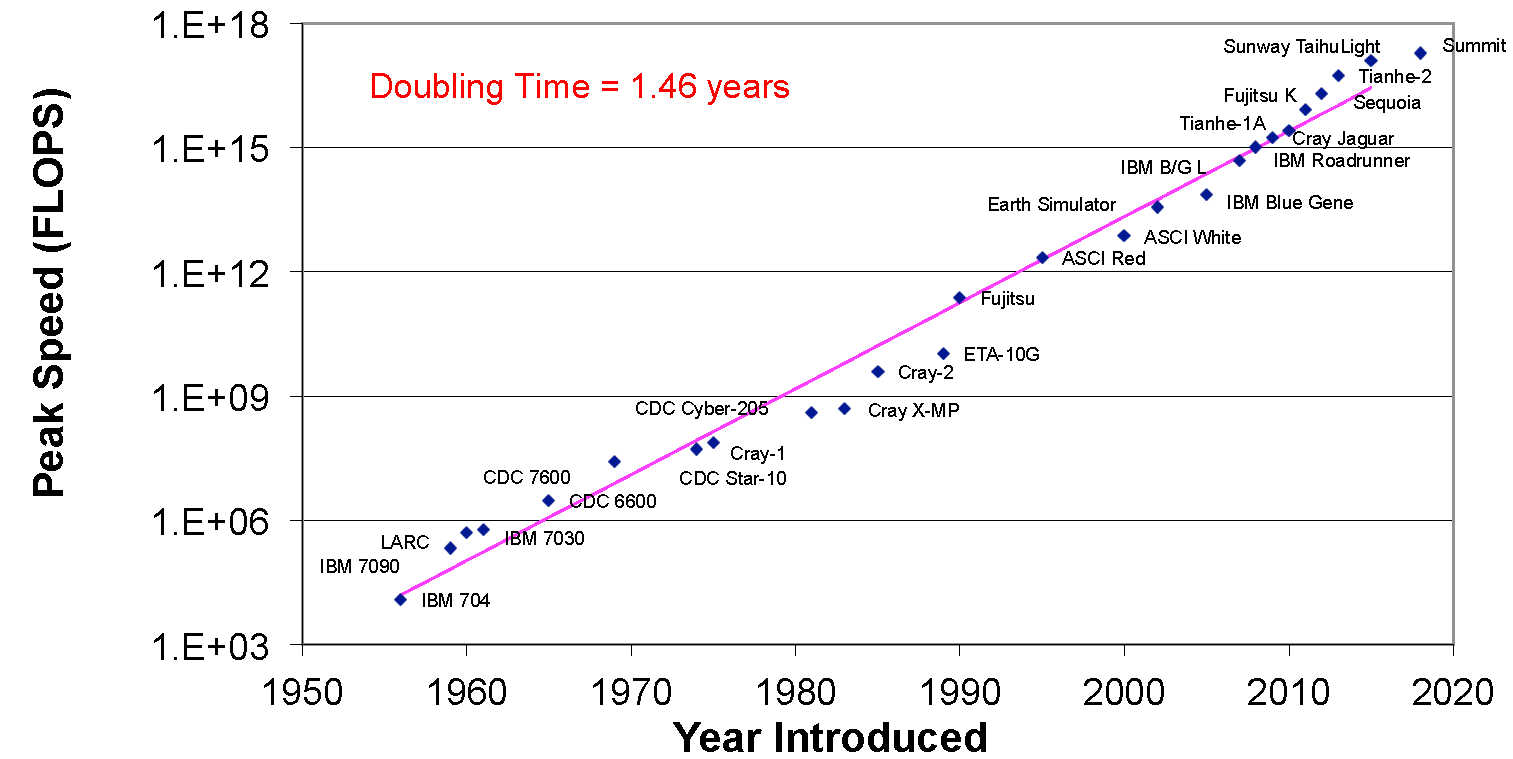
\includegraphics[width=6.3in]{fig/sc_evaluate.pdf}
	\caption{Top 1 Supercomputers' Performance by Year.}
		\label{sc_evaluate}
\end{figure}

The next barrier to overcome is the Exascale computing, which refers to computing systems capable of at least one exaFLOPS. This capacity represents a thousandfold increase over the first petascale computer which came into operation in 2008. The world first exascale supercomputer will come around 2020. China's first exascale supercomputer will enter service by 2020 according to the head of the school of computing at the National University of Defense Technology (NUDT). United States's first Exascale computer is planned to be built by 2021 at Argonne National Laboratory. The post-K announced by Japan will start the public service around 2021, and the first exascale supercomputer in Europe will appear around 2022. Exascale computing would be considered as a significant achievement in computer engineering, for it is estimated to be the order of processing power of the human brain at the neural level.

Considering the evaluation of HPC, there are always two questions proposed to the users:

\begin{itemize}
	\item How to build such powerful machines?
	\item How can the users develop applications to profit the computational capacity of supercomputers efficiently?
\end{itemize}

In order to answer these two questions above, this chapter firstly gives a glance at the modern computing architectures to build the supercomputers, and then different parallel programming models to develop the applications to benefit the whole computational power of these supercomputers.


\section{Modern Computing Architectures}

Different architectures of computing units are designed to build the supercomputers. In this section, the state-of-art of modern CPUs and accelerators are reviewed.

\subsection{CPU Architectures and Memory Access}

The \textit{Von Neumann architecture} is a computer architecture based on the description by the mathematician and physicist \textit{John von Neumann} and others in the \textit{First Draft of a Report on the EDVAC}. All the modern computing units are all envolved from this concept, which consists of five parts:

\begin{itemize}
	\item A \textit{processing unit} that contains an arithmetic logic unit and processor registers;
	\item A\textit{control unit} that contains an instruction register and program counter;
	\item \textit{Memory} that stores data and instructions;
	\item External mass \textit{storage};
	\item \textit{Input/output} mechanisms.
\end{itemize}

As shown in Fig. \ref{von-neumann}, the \textit{Von Neumann architecture} uses the shared bus between the program memory and data memory, which leads to its bottleneck. Since the single bus can only access one of the two types of memory at a time, the data transfer rate between the CPU and memory is rather low. With the increase of CPU speed and memory size,  the bottleneck has become more of a problem.

\begin{figure}[t]
	\centering
	\subfloat[Von Neumann architecture.]{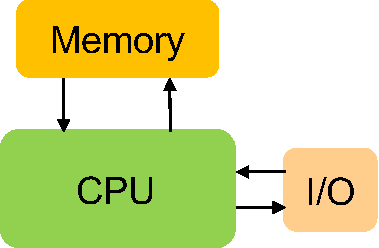
\includegraphics[width=1.8in]{fig/von-neumann.pdf}%
		\label{von-neumann}}
	\hspace{8.5pt}
	\subfloat[Harvard architecture.]{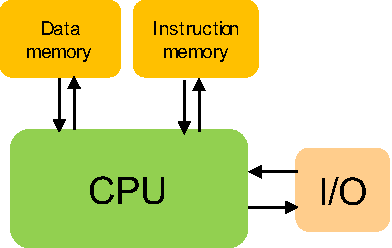
\includegraphics[width=1.8in]{fig/harvard.pdf}%
		\label{havard}}
	\hspace{8.5pt}
	\subfloat[Modified Harvard architecture.]{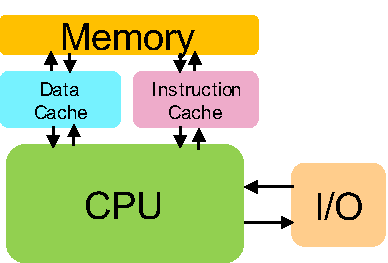
\includegraphics[width=1.8in]{fig/modified-harvard.pdf}%
	\label{modified-havard}}
	\caption{ Computer architectures.}
	\label{cpu-arch}
\end{figure}

The \textit{Harvard architecture} is another computer architecture with physically separate the storage and bus for the instructions and data. As shown in Fig. \ref{havard}, the limitation of a pure Harvard architecture is that the mechanisms must be provided to load the program to be executed into instruction memory separately and any data to be operated upon input memory. Additionally, read-only technology for the instruction memory allows the computer to begin execution of a pre-loaded program as soon as power is applied. The data memory will at this time be in an unknown state, so it is not possible to provide any kind of pre-defined data values to the program.

Today, most processors implement the separate pathways as \textit{Harvard architecture} to support the higher performance concurrent data and instruction access, meanwhile loosen the strictly separated storage between code and data. That is named as the \textit{Modified Havard architecture} (shown as Fig. \ref{modified-havard}). This model can be seen as the combination of the \textit{Von Neumann architecture} and  \textit{Harvard architecture}.

The solution is to provide a hardware pathway and machine language instructions so that the contents of the instruction memory can be read as if they were data. Initial data values can then be copied from the instruction memory into data memory when the program starts. If the data is not to be modified, it can be accessed by the running program directly from instruction memory without taking up space in the data memory.

Nowadays, most CPU has Von Neumann like unified address space and also separate instruction and data caches as well as memory protection, making them more Harvard-like, and so they could be classified more as \textit{modified Harvard architecture} even using unified address space.

\begin{figure}[htbp]
	\centering
	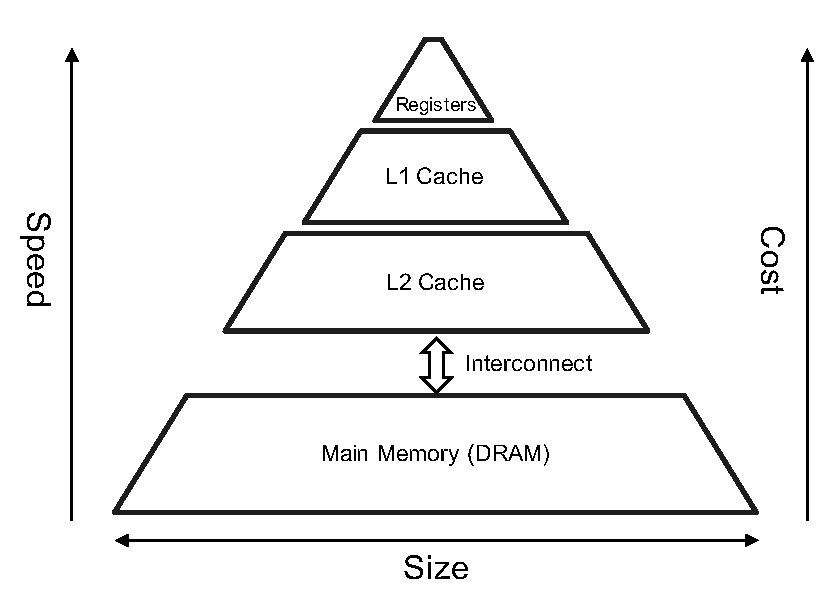
\includegraphics[width=4.6in]{fig/memory.pdf}
	\caption{Memory Hierarchy.}
	\label{fig:memory-access}
\end{figure}

The most common modification on \textit{modified Harvard architecture}  for modern CPUs is to build a memory hierarchy with a CPU cache separating instructions and data based on response time. As shown in Fig. \ref{fig:memory-access}, the top of the memory hierarchy which provides the fastest data transfer rate are the registers. Target data with arithmetic and logic operations will be temporarily held in the register to perform the computations. The number of registers is limited due to the cost. A CPU cache is a hardware cache used by CPU to reduce the average cost (time or energy) to access data from the main memory. A cache is a smaller, faster memory, closer to a processor core, which stores copies of the data from frequently used main memory locations. Most CPUs have different independent caches, including instruction and data caches, where the data cache is usually organized as a hierarchy of more cache levels. The lowest level is the main memory, which is made of Dynamic Radom-Acess Memory (DRAM) with the lowest bandwidth and the highest latency compared to registers and caches.

\subsection{Parallel Computer Memory Architectures}

The parallel computer memory architectures can be divided into shared and distributed memory types. The shared memory parallel computers vary widely, but generally have in common the ability for all processors to access all memory as global address space. Multiple processors can operate independently but share the same memory resources. Changes in a memory location effected by one processor are visible to all other processors. Historically, shared memory machines have been classified as \textit{Uniform Memory Access (UMA)} (shown as \ref{uma}) and \textit{Non-Uniform Memory Access (NUMA)} (shown as \ref{numa}), based upon memory access times. UMA is most commonly represented today by Symmetric Multiprocessor (SMP) machines with Identical processors. These processors require Equal access and access times to memory. NUMA Often made by physically linking two or more SMPs, one SMP can directly access memory of another SMP. Not all processors have equal access time to all memories, memory access across link is slower. The advantages of shared memory architectures are: 1) Global address space provides a user-friendly programming perspective to memory; 2) Data sharing between tasks is both fast and uniform due to the proximity of memory to CPUs. The disadvantages are: 1) the lack of scalability between memory and CPUs, in fact, adding more CPUs can geometrically increases traffic on the shared memory-CPU path, and for cache coherent systems, geometrically increase traffic associated with cache/memory management; 2) Programmer responsibility for synchronization constructs that ensure "correct" access of global memory. There is no way we can reach the hundreds of thousands of CPU-cores we need for today’s multi-petaflop supercomputers.

\begin{figure}[t]
	\centering
	\subfloat[Shared Memory Architecture (UMA).]{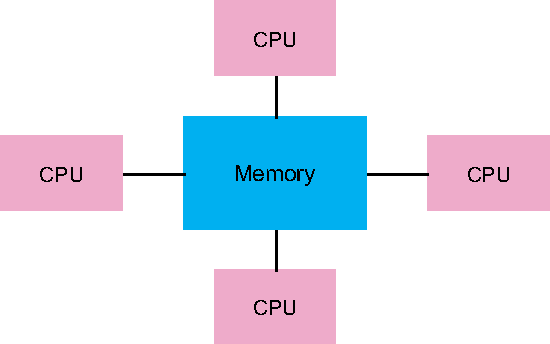
\includegraphics[width=2.6in]{fig/uma.pdf}%
		\label{uma}}
	\hspace{34.5pt}
	\subfloat[Shared Memory Architecture (NUMA)]{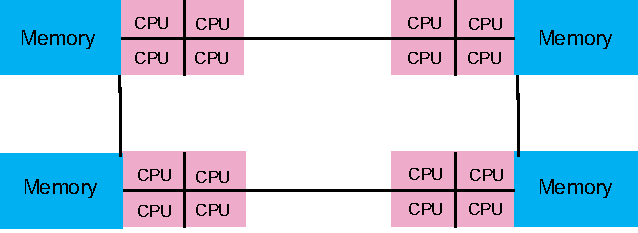
\includegraphics[width=2.6in]{fig/numa.pdf}%
		\label{numa}}
		\hspace{11.5pt}
		\subfloat[Distributed Memory Architectures.]{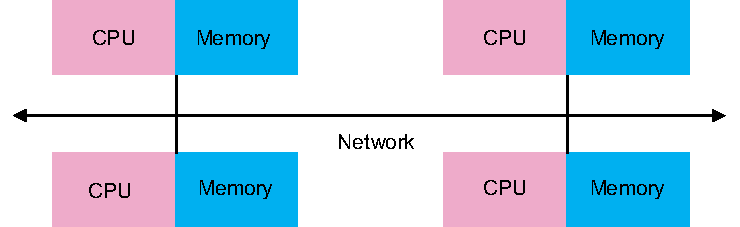
\includegraphics[width=3.1in]{fig/distributed.pdf}%
		\label{distributed}}
	\hspace{1.5pt}
	\subfloat[Distributed Shared Memory Architectures.]{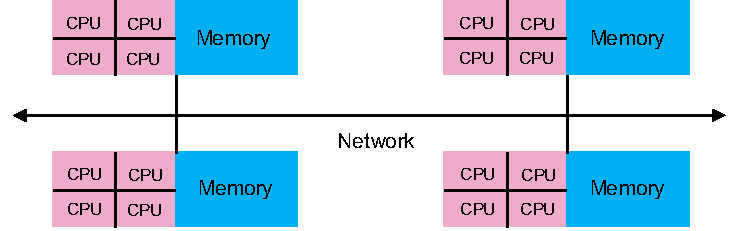
\includegraphics[width=3.1in]{fig/hybrid.pdf}%
		\label{hybrid}}
	\caption{Parallel Computer Memory Architectures.}
	\label{parallel-memory}
\end{figure}

Then the distributed-memory architecture is proposed, which takes many multicore computers and connects them together using a network, much like workers in different offices communicating by telephone. With a sufficiently fast network we can in principle extend this approach to millions of CPU-cores and beyond. As shown in Fig. \ref{distributed}, inside distributed memory system, processors have their own local memory. Memory addresses in one processor do not map to another processor, so there is no concept of global address space across all processors. Because each processor has its own local memory, it operates independently. Changes it makes to its local memory have no effect on the memory of other processors. Hence, the concept of cache coherency does not apply. When a processor needs access to data in another processor, it is usually the task of the programmer to explicitly define how and when data is communicated. Synchronization between tasks is likewise the programmer's responsibility. The advantages of distributed memory architecture are: 1) Memory is scalable with the number of processors. Increase the number of processors and the size of memory increases proportionately; 2) Each processor can rapidly access its own memory without interference and without the overhead incurred with trying to maintain global cache coherency; 3) Cost effectiveness. The disadvantages are: 1) the programmer is responsible for many of the details associated with data communication between processors; 2) It may be difficult to map existing data structures, based on global memory, to this memory organization; 3) Non-uniform memory access times - data residing on a remote node takes longer to access than node local data.

Nowadays, the largest and fastest computers in the world employ both shared and distributed memory architectures (shown as Fig. \ref{hybrid}). The shared memory component can be a shared memory machine and/or graphics processing units (GPU). The distributed memory component is the networking of multiple shared memory/GPU machines, which know only about their own memory - not the memory on another machine. Therefore, network communications are required to move data from one machine to another. Current trends seem to indicate that this type of memory architecture will continue to prevail and increase at the high end of computing for the foreseeable future.

In a word, Shared-memory systems are difficult to build but easy to use, and are ideal for laptops and desktops. Distributed-shared memory systems are easier to build but harder to use, comprising many shared-memory nodes with their own separate memory. Distributed-shared memory systems introduce much more hierachical memory and computing with multi-level of parallelism. The important advantage of distributed-shared memory architectures is increasing scalability, and the important disadvantage is increasing the complexity to program.

\subsection{Nvidia's GPGPU}

General-purpose computing on graphics processing units (GPGPU, rarely GPGP) is the use of a graphics processing unit (GPU), which typically handles computation only for computer graphics, to perform computation in applications traditionally handled by the central processing unit (CPU). GPU was first introduced as a specialized electronic circuit designed to rapidly manipulate and alter memory to accelerate the creation of images in a frame buffer intended for output to a display device. Modern GPUs are very efficient at manipulating computer graphics and image processing. Due to its special functionality, GPGPU serves as an accelerator of CPU to improve the overall performance of computers. Nowadays, it is becoming increasingly common to use GPGPU to build the supercomputers. Until now, 5 of top 10 supercomputers in the world use GPGPU.

\begin{figure}[htbp]
	\centering
	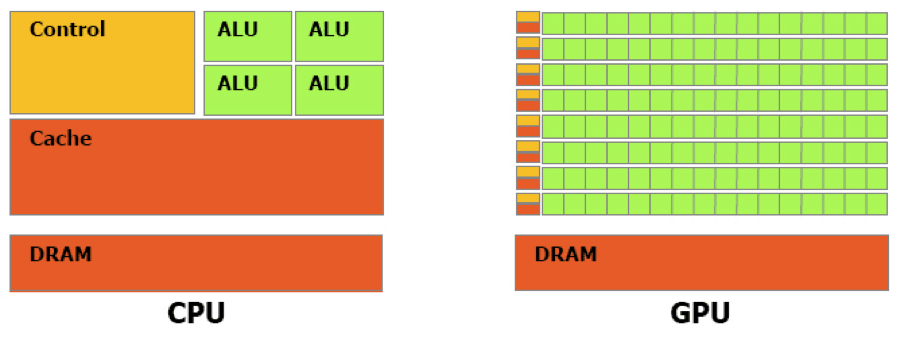
\includegraphics[width=6.in]{fig/cpu_vs_gpu.png}
	\caption{CPU vs GPU.}
	\label{cpuvsgpu}
\end{figure}

As shown in Figure \ref{cpuvsgpu}, the architectures of CPU and GPU are different: the CPU has a small number of complex cores and massive caches while the GPU has thousands of simple cores and small caches. These ALUs of GPU are simple, data-parallel, multi-threaded which offer high computing power and large memory bandwidth. In brief, graphics chips are designed for parallel computations with lots of arithmetic operations, and CPUs are for general complex applications. The host character of the CPU requires complicated cores and deep pipelines to deal with all kinds of operations. It usually runs at a higher frequency and supports branch prediction. The GPU only focuses on data-parallel image renderings thus the pipeline is shallow. The same instructions are used on large datasets in parallel with thousands of hardware cores, so the branch prediction is not necessary, and memory access latency is hidden by important arithmetic operations instead of caching. GPGPU is also regarded as a powerful backup to overcome the \textit{power wall}.

Introduced in mid-2017, the newest Tesla V100 card can deliver $7.8$ TFLOPS in double-precision floating point and $15.7$ TFLOPS for single-precision.

\subsection{Intel's Many Integrated Cores}

The performance improvement of processors comes from the increasing number of computing units within the small chip area. Thanks to advanced semiconductor processes, more transistors can be built in one shared-memory system to do multiple things at once: from the view of programmers, this can be realized in two ways: different data or tasks execute in multiple individual computing units (multi-thread) or long uniform instruction decoders (vectorization).

\begin{figure}[htbp]
	\centering
	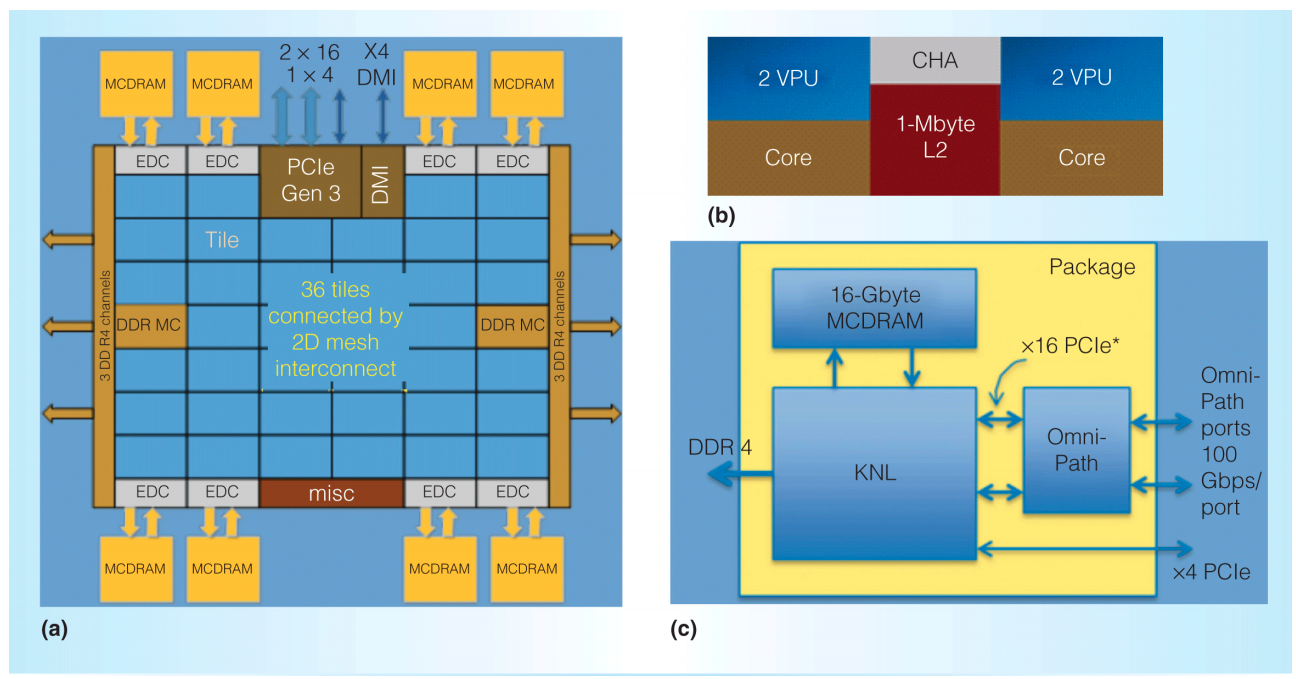
\includegraphics[width=6.2in]{fig/KNL1.png}
	\caption{The organization of a Knights Landing processor.}
	\label{knl1}
\end{figure}

Intel officially first revealed the latest MIC codenamed Knights Landing (KNL) in 2013. Being available as a coprocessor like previous boards, KNL can also serve as a self-boot MIC processor that is binary compatible with standard CPUs and boot
standard OS. These second generation chips could be used as a standalone CPU, rather than just as an add-in card. Another key feature is the on-card high-bandwidth memory (HBM) which provides high bandwidth and large capacity to run large HPC workloads. Memory bandwidth is one of the common performance bottlenecks for computational applications due to the memory wall. KNL implements a two-level memory system to address this issue. It shares application areas with GPUs. The main difference between Xeon Phi and a GPGPU like Nvidia Tesla is that Xeon Phi, with an x86-compatible core, can, with less modification, run software that was originally targeted at a standard x86 CPU.

\subsection{Others}

There are also processors designed for supercomputing, for example, the SW26010 and Matrix-2000. The SW26010 is a 260-core manycore processor \cite{fu2016sunway} designed by the National High-Performance Integrated Circuit Design Center in Shanghai. It implements the Sunway architecture, a 64-bit reduced instruction set computing (RISC) architecture designed by China. The SW26010 has four clusters of 64 Compute-Processing Elements (CPEs) which are arranged in an eight-by-eight array. The CPEs support SIMD instructions and are capable of performing eight double-precision floating-point operations per cycle. Each cluster is accompanied by a more conventional general-purpose core called the Management Processing Element (MPE) that provides supervisory functions. Each cluster has its own dedicated DDR3 SDRAM controller and a memory bank with its own address space. The processor runs at a clock speed of 1.45.

Matrix-2000 \cite{zhang2018mocl} is a 64-bit 128-core many-core processor designed by NUDT and introduced in 2017. This chip was designed exclusively as an accelerator for China's Tianhe-2 supercomputer in order to upgrade and replace the aging Intel's Knights Corner accelerators. The Matrix-2000 features 128 RISC cores operating at 1.2 GHz achieving 2.46/4.92 TFLOPS (DP/SP) with a peak power dissipation of 240W. The Matrix-2000 consists of 128 cores, eight DDR4 memory channels, and x16 PCIe lanes. The chip consists of four supernodes (SN) consisting of 32 cores each operating at 1.2 GHz with a peak power dissipation of 240 Watts.

\section{Parallel Programming Model}

After the introduction of hardware architectures, we will present the different parallel programming models on top of them in this section.

\subsection{OpenMP}
OpenMP (Open Multi-Processing) \cite{dagum1998openmp} is an application programming interface (API) that supports multi-platform shared memory parallel programming in C, C++, and Fortran. OpenMP supports most platforms, instruction set architectures, and operating systems. It consists of a set of compiler directives, library routines, and environment variables. OpenMP provides the capability to incrementally parallelize a serial program with by inserting the specific directives. These directives can be ignored by the compiler, and the application can be executed in a sequential way when target machines do not support OpenMP. OpenMP is designed for multi-processor/core, shared memory machines. The underlying architecture can be shared memory UMA or NUMA. OpenMP programs accomplish parallelism exclusively through the use of threads.

\begin{figure}[htbp]
	\centering
	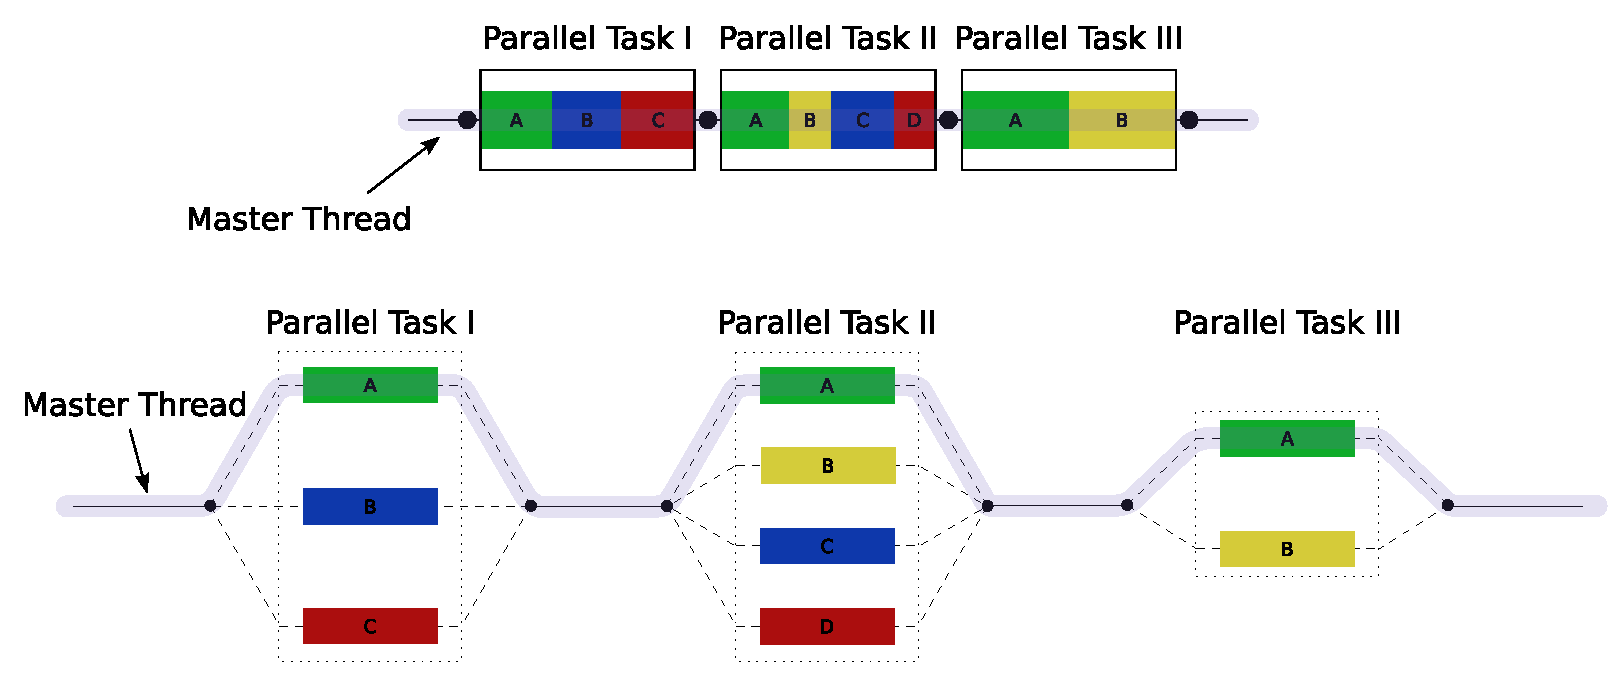
\includegraphics[width=6.3in]{fig/Fork_join.pdf}
	\caption{OpenMP \textbf{fork-join} Model.}
	\label{openmp_fork_join}
\end{figure}

As shown in Fig. \ref{openmp_fork_join}, OpenMP uses the \textbf{fork-join} model to support parallel execution. All OpenMP programs begin with a single process which executes utils sequentially the first parallel region construct is encountered.  Then this thread creates a team of parallel threads and distributes the workload to them in order to have them work simultaneously. When the team threads complete the statements in the parallel region construct, they synchronize and terminate, leaving only the master thread. The new released OpenMP begins to support task scheduling strategies, the SIMD directives for high-level vectorization and the \textit{offload} directives for heterogeneous systems.

\subsection{CUDA}

CUDA (Compute Unified Device Architecture) \cite{nvidia2011nvidia} is a parallel programming platform and application programming interface model created by Nvidia. It allows software developers and software engineers to use a CUDA-enabled GPU for general purpose processing. The CUDA software layer gives direct access to GPU's virtual instruction set de parallel computational elements, for the execution of compute kernels. The CUDA platform is designed to work with programming languages such as C, C++, and Fortran. This accessibility makes it easier for specialists in parallel programming to use GPU resources. CUDA supports programming frameworks such as OpenACC and OpenCL.

\begin{figure}[htbp]
	\centering
	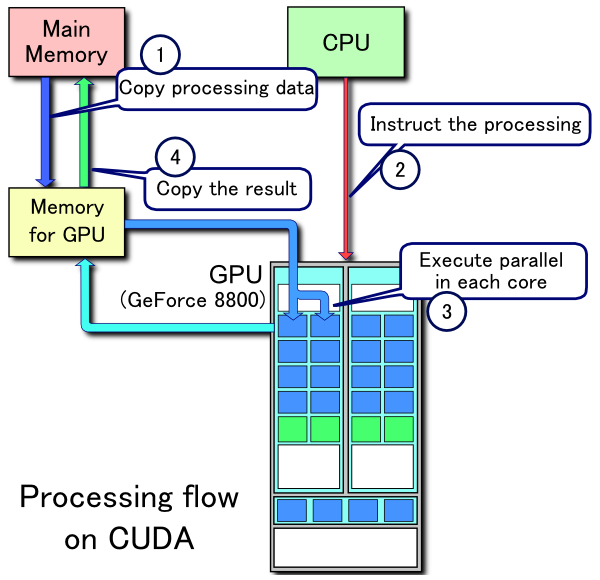
\includegraphics[width=4.2in]{fig/CUDA.png}
	\caption{Processing flow on CUDA.}
	\label{cuda_flow}
\end{figure}

\subsection{Message Passing Interface}

MPI (Message Passing Interface) \cite{gropp1999using} is a standardized and portable message-passing standard designed by a group of researchers from academia and industry to support a wide variety of parallel computing architectures. MPI provides a simple-to-use portable interface for the basic user, yet one powerful enough to allow programmers to use the high-performance message passing operations available on advanced machines. Most MPI implementations consist of a specific set of routines directly callable from C, C++, Fortran and any language able to interface with such libraries. The MPI interface is meant to provide essential virtual topology, synchronization, and communication functionality between a set of processes (that have been mapped to nodes/servers/computer instances) in a language-independent way, with language-specific syntax (bindings), plus a few language-specific features. 

\begin{figure}[htbp]
	\centering
	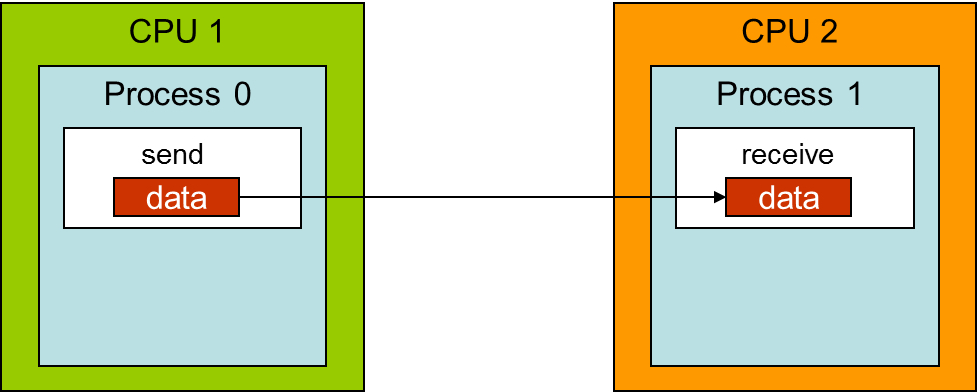
\includegraphics[width=5.4in]{fig/mpi_send_recv.jpg}
	\caption{MPI send and receive Model.}
	\label{mpi_model}
\end{figure}

MPI library functions include, but are not limited to, basic point-to-point send/receive operations, collective functions involving communication among all processes, synchronizing nodes (barrier operation), the one-sided communication, dynamic process management, I/O and so on. Point-to-point operations support both the communication in both synchronous and asynchronous ways. In modern computing platform with multiple shared-memory nodes, the shared memory programming models such as OpenMP and message passing programming such as MPI can be considered as complementary programming approaches, and can occasionally be used together in a hybrid way.

\subsection{Partitioned Global Address Space}

In computer science, a partitioned global address space (PGAS) is a parallel programming model. It assumes a global memory address space that is logically partitioned and a portion of it is local to each process, thread, or processing element. The novelty of PGAS is that the portions of the shared memory space may have an affinity for a particular process, thereby exploiting locality of reference. There are different implementation based on PGAS model, such as Unified Parallel C, Coarray Fortran, Split-C, Chapel, X10, UPC++, DASH, XcalableMP, etc. PGAS attempts to combine the advantages of an SPMD programming style for distributed memory systems (as employed by MPI) with the data referencing semantics of shared memory systems. This is more realistic than the traditional shared memory approach of one flat address space because hardware-specific data locality can be modeled in the partitioning of the address space.

\subsubsection{XcalableMP}

XcalableMP \cite{lee2010implementation} is a language extension of C and Fortran for parallel programming on distributed memory systems that help users to reduce those programming efforts. XcalableMP provides two programming models. The first one is the global view model, which supports typical parallelization based on the data and task parallel paradigm, and enables parallelizing the original sequential code using minimal modification with simple, OpenMP-like directives. The other one is the local view model, which allows using CAF-like expressions to describe inter-node communication. Users can even use MPI and OpenMP explicitly in our language to optimize performance explicitly.

\subsection{Task/Graph Based Parallel Programming}

With the increase of the complexity of applications on the supercomputers, it is more and more difficult for the developers to maintain the parallel codes on the modern computing architectures. The task/graph based parallel programming models are proposed to express the task parallelism and data dependencies of complex codes. In this section, we list several well-known task/graph based parallel programming models.

\subsubsection{YML}

YML \cite{delannoyyml} allows you to transparently use one or more grid middleware to run an application. For this, the project is based on a dedicated language named YvetteML. YML can describe a complex parallel application regardless of the execution platform. The YvetteML language is used to express the task graph of the application. The nodes of the graph are the tasks described by components, and the edges correspond to dependencies or communications. The components are written in XML. Each component implementation can contain C ++, XMP-C, XMP-FORTRAN or other code. Each component implementation can be expressed with finer grain parallelism.

\subsubsection{StarPU}

StarPU\footnote{http://starpu.gforge.inria.fr} \cite{augonnet2011starpu} is a task programming library for hybrid architectures. The application provides algorithms and constraints:
\begin{itemize}
	\item CPU/GPU implementations of tasks;
	\item A graph of tasks, using either the StarPU's high-level GCC plugin pragmas, StarPU's rich C/C++ API, or OpenMP pragmas.
\end{itemize}

StarPU handles run-time concerns:
\begin{itemize}
	\item Task dependencies;
	\item Optimized heterogeneous scheduling;
	\item Optimized data transfers/replication between main memory and discrete memories;
	\item Optimized cluster communications.
\end{itemize}
\subsubsection{Swift}

Swift\footnote{http://swift-lang.org/main/index.php} \cite{wilde2011swift} is a data-flow oriented coarse-grained scripting language that supports dataset typing and mapping, dataset iteration, conditional branching, and procedural composition. Swift programs (or workflows) are written in a language called Swift. Swift scripts are primarily concerned with processing (possibly large) collections of data files, by invoking programs to do that processing. Swift handles execution of such programs on remote sites by choosing sites, handling the staging of input and output files to and from the chosen sites and remote execution of programs.

\subsubsection{Legion}

Legion\footnote{http://legion.stanford.edu} \cite{grimshaw1994synopsis} is a data-centric parallel programming system for writing portable high performance programs targeted at distributed heterogeneous architectures. Legion presents abstractions which allow programmers to describe properties of program data (e.g., independence, locality). By making the Legion programming system aware of the structure of program data, it can automate many of the tedious tasks programmers currently face, including correctly extracting task- and data-level parallelism and moving data around complex memory hierarchies. A novel mapping interface provides explicit programmer controlled placement of data in the memory hierarchy and assignment of tasks to processors in a way that is orthogonal to correctness, thereby enabling easy porting and tuning of Legion applications to new architectures.


\section{Exascale Challenges of Supercomputers}

 (\textcolor{red}{This section need be rewritten})
 
According to Moore's law, the number of transistors per integrated circuit doubles every $2$ years, which means that the size of the transistor is reduced to half. Moore's law is found to be acceptable utils 2002. Since then, the overheating introduced by higher frequency reaches the limit of air cooling. This is the famous \textit{power wall}. The modern architectures with multiple processors on-chip, lower operating frequency and hierarchical architectures come, such as the GPU, MIC, SW26010, and Matrix-2000.

\begin{figure}[htbp]
	\centering
	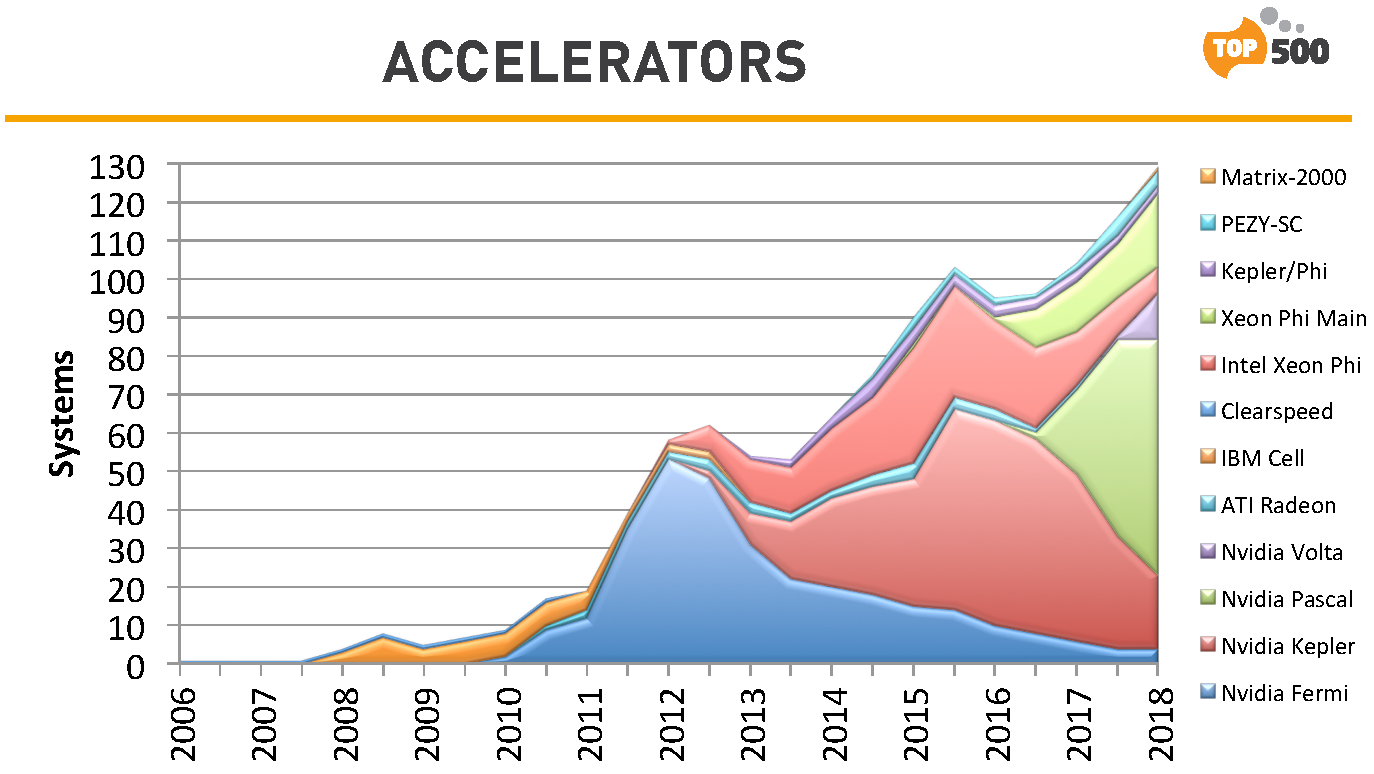
\includegraphics[width=6.6in]{fig/top500.pdf}
	\caption{Top 1 Supercomputers' Performance by Year.}
	\label{top500-acc}
\end{figure}

\begin{itemize}
	\item Highly hierarchical architectures of computing and memory;
	\item Increasing levels and degree of parallelism;
	\item Heterogeneity of computing, memory, and scalability;
	\item Requirement of parallel programming:
	\begin{itemize}
		\item multi-grain;
		\item multi-level memory;
		\item reducing synchronizations and promoting asynchronicity;
		\item multi-level scheduling strategies.
	\end{itemize}
\end{itemize}


\clearemptydoublepage

\chapter{Krylov Subspace Methods}\label{Krylov Subspace Methods}

\begin{displayquote}
	\textsf{An important application on supercomputers is to solve the linear systems and eigenvalue problems. The chapter gives an overview of the relevant iterative methods to solve large-scale non-Hermitian linear systems and eigenvalue problems. Many applications in science and engineering fields can be formulated as such problems with large dimensions.  Large matrices that arise in most applications are almost always sparse. That is, the vast majority of their entries are zero. In numerical linear algebra, these systems are often solved by iterative methods. An iterative method is a mathematical procedure that uses an initial guess to generate a sequence of improving approximate solutions for a class of problems, in which the $n$-th approximation is derived from the previous ones. Krylov subspace methods are very useful and popular iterative methods to solve large-scale sparse systems since their simplicity and generality. In this chapter, firstly we give a summary on the existing stationery and non-stationary iterative methods, especially the Krylov subspace methods. Then, the mathematical definition of GMRES to solve non-Hermitian linear systems and Arnoldi methods to solve non-Hermitian eigenvalue problems are given in details. For some applications, the convergence of conventional Krylov subspace methods cannot always be guaranteed. Thus various kinds of preconditioners to accelerate the convergence are introduced. In the end, this chapter gives a survey on the parallel implementation on distributed memory platforms, and also the related challenges on the upcoming exascale supercomputers. The material covered in this chapter will be helpful in establishing the mathematical base of this dissertation. Additionally, a large part of consistent efforts in this field are reviewed in this chapter, even some of them have less connection with the motivation of this thesis.}
\end{displayquote}

\vspace{0.6in}

\section{Linear Systems and Eigenvalue Problems}

Given a matrix $A$ $\in \mathbb{C}^{n \times n}$ and a $n$-vector $b$ $\in \mathbb{C}^{n}$, the problem considered is: Find $x \in \mathbb{C}^{n}$ such that:

\begin{equation}
\label{ax=b1}
Ax=b.
\end{equation}

This problem is a \textit{linear system}, $A$ is the coefficient matrix, $b$ is the \textit{right hand side (RHS)}, and $x$ is the \textit{vector of unknowns}. In most cases, the linear systems are formatted by solving complex Partial Differential Equations (PDEs) systems. In general, the discretization of these PDEs into a cell-centered Finite Volume scheme in space and an Euler implicit method in time, leads to a nonlinear system which can be solved with a Newton’s method. For each Newton step by time, the system is linearized then solved using a linear solver.

\textit{Eigenvalue problems} occur in many areas of science and engineering, such as structural analysis and electromagnetic applications, and $eigenvalues$ are also important in analyzing numerical methods. The standard eigenvalue problem can be defined as: given a matrix $A$ $\in \mathbb{C}^{n \times n}$, find scalar $\lambda \in \mathbb{C}$ and nonzero vector $v \in \mathbb{C}$ such that:

\begin{equation}
\label{av=lv}
Av=\lambda v.
\end{equation}

In this formula, $\lambda$ is an \textit{eigenvalue} of $A$, and $v$ is its corresponding \textit{eigenvector}, $\lambda$ may be complex even if $A$ is real. The \textit{spectrum} of $A$ is the set of all eigenvalues of $A$, denoted it as $\lambda(A)$, and the \textit{Spectral radius} of $A$ $\rho(A)$ is $\max\{|\lambda|: \lambda \in \lambda(A)\}$. 

\section{Iterative Methods}

Iterative methods approach the solution $x$ of Equation (\ref{ax=b1}) by a number of steps. Compared with the direct methods such as LU and Gauss Jordan which need an overall computational cost of the order $\frac{2}{3}n^3$, the cost of iterative methods is the order of $n^2$ operations for each iteration. Iterative methods are especially competitive with direct methods in the case of large sparse matrices, with the potential introduction of the dramatic fill-in by the direct methods. This section gives an overview of both stationary and non-stationary iterative methods.

\subsection{Stationary and Multigrid Methods}

The iterate of stationnary methods to solve Equation (\ref{ax=b1}) can be expressed in the simple form
\begin{equation}
\label{stationary}
x_k = Bx_{k-1}+c
\end{equation}

where neither $B$ nor $c$ depends upon the iteration count $k$. The four well-known stationary methods are the \textit{Jacobi method} (\cite{yang2014acceleration}), \textit{Gauss-Seidel method} (\cite{yoon1988lower}), \textit{successive overrelaxation method (SOR)} (\cite{adams1982multi}), and \textit{symmetric successive overrelaxation method (SSOR)} (\cite{axelsson1972generalized}). Beginning with an initial guess vector, these methods modify one or a few components of the approximation at each iterative step, until the convergence is reached. These medications are called relaxation steps. Theoretically, the stationary methods are applicable for all linear systems, but they are more efficient only for the applications arise from the finite difference discretization of Ellipse Partial Differential Equations. Though the inefficiency of stationary methods for most linear problems, they are often used by combining with the more efficient methods described in later sections of this chapter.

For \textbf{Jacobi method}, the Formula (\ref{stationary}) is extended as:

\[x_k = D^{-1}(L+U)x_{k-1}+D^{-1}b\]

Where the matrices $D$, $-L$, and $-U$ represent the diagonal, strictly lower triangular, and strictly upper triangular parts of A, respectively. The convergence condition for the Jacobi method is when the spectral radius of the matrix $D^{-1}(L+U)$ is less than 1:

\[\rho(D^{-1}(L+U)) < 1\]

For general cases, the convergence of Jacobi method can be slow. A sufficient (but not necessary) condition for the convergence is that the matrix A is strictly or irreducibly diagonally dominant.

For \textbf{Gauss-Seidel method}, the Formula (\ref{stationary}) is extended as:

\[x_k = (D-L)^{-1}(Ux_{k-1}+b)\]

Where the matrices $D$, $-L$, and $-U$ represent the diagonal, strictly lower triangular, and strictly upper triangular parts of A, respectively. The Gauss-Seidel method is similar to the Jacobi method except that it uses updated values as soon as they are available. It generally converges faster than the Jacobi method, although still relatively slow. 
The Gauss-Seidel method can converge if either:
\begin{enumerate}
	\item The matrix $A$ is strictly or irreducibly diagonally dominant, or
	\item $A$ is symmetric positive-definite.
\end{enumerate}

For \textbf{SOR method}, the Formula (\ref{stationary}) is extended as:

\[ x_{k}=(D-\omega L)^{-1}[\omega U+(1-\omega)D]x_{k-1}+\omega(D-\omega L)^{-1}b\]

Where the matrices $D$, $-L$, and $-U$ represent the diagonal, strictly lower triangular, and strictly upper triangular parts of A, respectively. The SOR method can be derived from the Gauss-Seidel method by introducing an extrapolation parameter $\omega$. If $\omega$, the SOR method simplifies to the Gauss-Seidel method. A theorem due to Kahan (1958) shows that SOR fails to converge if $\omega$ is outside the interval $(0,2)$. In general, it is not possible to compute in advance the value of $\omega$ that will maximize the rate of convergence of SOR. This method can converge faster than Gauss-Seidel by order of magnitude.

Finally, \textbf{SSOR method} is useful as a preconditioner for other methods. However, it has no advantage over the SOR method as a stand-alone iterative method.

In general, many stationary methods have the smoothing property, where oscillatory modes with short wave-length of the errors of linear systems can be eliminated effectively, but the smooth modes with long wave-length are damped very slowly. Thus \textbf{multigrid (MG) methods} (\cite{hutchinson1986multigrid, hiptmair1998multigrid, bank1988hierarchical}) are introduced for solving differential equations using a hierarchy of discretizations. The main idea of MG methods is to accelerate the convergence of stationary iterative methods (known as relaxation process) by a global correction on the approximative solution of the fine grid from time to time. This global correction is achieved by solving a coarse problem. The coarse grids can be used to compute an improved initial guess for the fine-grid processes. The reason for the coarse grid are:

\begin{enumerate}
	\item Relaxation on the coarse-grid is much cheaper;
	\item Relaxation on the coarse-grid has a marginally better convergence rate;
	\item Smooth error is relatively more oscillatory in the coarse-grid processes, and the relaxation will be more effective
\end{enumerate}

The steps $2-4$ in Algorithm \ref{alg:v-cycle} is the kernel of multigrid method, which gives the restriction-corse solution-interpolation processus. The invovled matrices in this algorithm are:
\[A=A_h=orginal \ matrix\]
\[R=R_h^{2h}=restriction \ matrix\]
\[I=I_h^{2h}=interpolation \ matrix\]
\[A_{2h}=R_h^{2h}A_hI_{2h}^h=RAI=coarse \ grid \ matrix\]

\begin{algorithm}[htbp]{}
	\caption{Fine-corse-fine loop of multigrid method}   
	\label{alg:v-cycle}   
	\begin{algorithmic}[1]
		
		\State Relaxion \textbf{Iterate} on $A_hu=b_h$ by stationary methods to reach $u_k$.
		\State \textbf{Restrict} the residual $r_h = b_h - A_hu_h$ to the coarse grid by $r_{2h}=R_h^{2h}r_h$.
		\State \textbf{Solve} $A_{2h}E_{2h}=r_{2h}$.
		\State \textbf{Interpolate} $E_{2h}$ as $E_h=I^{h}_{2h}E_{2h}$. Add $E_h$ to $u_h$.
		\State \textbf{Iterative} more times on $A_hu=b_h$ starting from the improved $u_h+E_h$.
		
	\end{algorithmic}  
\end{algorithm}


One extension of multigrid method is the \textbf{algebraic multigrid methods (AMG)} (\cite{ruge1987algebraic, vanvek1996algebraic, brandt1986algebraic,brezina2001algebraic}). AMG construct their restriction, interpolation, and coarse grid matrices directly from the matrix of a linear system. AMG is regarded as advantageous when geometric multigrid is too difficult to apply, e.g., unstructured meshes, graph problem, etc.  Fig. \ref{multilevel-amg} gives an example of hierarchical multi-level AMG.

\begin{figure}[htbp]
	\centering
	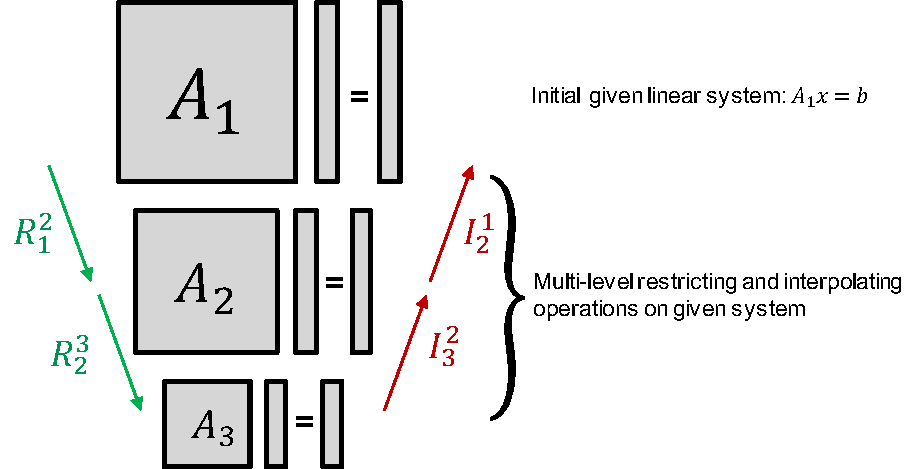
\includegraphics[width=5.6in]{fig/multilevel-amg.pdf}
	\caption{Algebraic multigrid hierarchy.}
	\label{multilevel-amg}
\end{figure}

\subsection{Non-stationary Methods}

In practice, the stationary methods talked in the last section cannot always get the convergence quickly for more general matrices which are not constructed from the Ellipse PDEs. The GMG and AMG which use the relaxation steps of stationary methods' can speed up the convergence for more general matrices, but the construction of restriction, interpolation, and coarse matrices either from geometric PDE problems or the operator matrix $A$ is far more difficult, and these operations matter the convergence. There is no free lunch for AMG which is hard to "control" and get optimal performance. In my dissertation, I will talk more about the \textbf{non-stationary methods} which are easy to implement and have better convergence performance than the stationary methods. The difference of non-stationary methods comparing with stationary methods is that the involved computational information changes at each step of the iteration. The most well-known non-stationary methods are the suite of \textbf{Krylov subspace methods}.

\section{Krylov Subspace methods}

This section presents the Krylov Subspace projection and the basic Arnoldi reduction in the Krylov subspace.

\subsection{Krylov Subspaces}
In linear algebra, the $m$-order Krylov subspace (\cite{saad1981krylov}) generated by a $n\times n$ matrix $A$ and a vector $b$ of dimension $n$ is the linear subspace spanned by the images of $b$ under the first $m$ powers of $A$, that is 
\[K_m(A,b)=span (b, Ab, A^2b,\cdots, A^{m-1}b).\] 

The Krylov subspace provides the ability to extract the approximations from an m-dimensional subspace $K_m$. Since $K_m$ is the subspace of all vectors in $\mathbb{R}^n$, it can be written as $x=p(A)b$, with $p$ a polynomial of degree not exceeding $m-1$.

\subsection{Basic Arnoldi Reduction}

\begin{algorithm}[htbp]{}
	\caption{Arnoldi Reduction}   
	\label{alg:arnoldi-reduction}   
	\begin{algorithmic}[1]
		\Function {AR}{$input$:$A,m,\nu$, $output$: $H_m, \Omega_m$}
		\State $\omega_1=\nu /||\nu||_2$
		\For {\texttt{$j=1, 2, \cdots, m$}}
		\For{$i=1,2,\cdots,j$}
		\State $h_{i,j}=(A\omega_j,\omega_i)$
		\EndFor
		\State $\omega_j=A\omega_j-\sum_{i=1}^jh_{i,j}\omega_i$
		\State $h_{j+1,j}=||\omega_j||_2$
		\If {$h_{j+1,j}=0$} Stop
		\EndIf
		\State $\omega_{j+1}=\omega_j/h_{j+1,j}$
		\EndFor 
		\EndFunction
	\end{algorithmic}  
\end{algorithm}

Arnoldi procedure is well used to build an orthogonal basis of the Krylov subspace $K_m$. One variant of basic Arnoldi reduction algorithm is given in Algorithm \ref{alg:arnoldi-reduction}. In this algorithm, at each step of Arnoldi reduction, the algorithm times the previous Arnoldi vector $\omega_j$ by matrix $A$, and get an orthogonal vector $\omega_j$ against all previous $\omega_i$ by a stand Gram-Schmit procedure. It will stop if the vector computed in line $5$ is zero. Then the vectors $\omega_1, \omega_2. \cdots, \omega_m$ form an orthonormal basis of the Krylov Subspace. 

\begin{figure}[htbp]
	\centering
	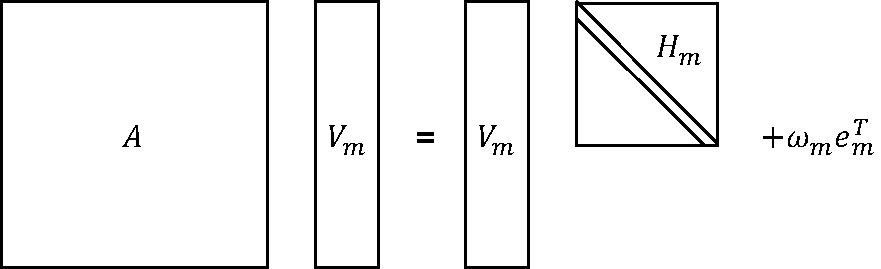
\includegraphics[width=5.8in]{fig/arnoldi_reduction.pdf}
	\caption{ The action of $A$ on $V_m$ gives $V_mH_m$ plus a rank-one matrix.}
	\label{arnoldi}
\end{figure}

Denote by $V_m$, the $n \times m$ matrix with column vectors $\omega_1, \omega_2. \cdots, \omega_m$, by $\overline{H}_m$, the $(m+1) \times m$ Hessemberg matrix whose nonzero entries $h_{i,j}$ are defined by  Algorithm \ref{alg:arnoldi-reduction}, then note $H_m$ as the matrix obtained from  $\overline{H}_m$ by deleting its last row (shown as Fig. \ref{arnoldi}). The following relations are given:
\begin{equation}
AV_m = V_m H_m + \omega_me_m^T = V_{m+1}\bar{H}_m.
\end{equation}

\begin{equation}
V_m^T A V_m = H_m.
\end{equation}

In case that the norm of $\omega_j$ in line $5$ of  Algorithm \ref{alg:arnoldi-reduction} vanishes at a certain step $j$, the next vector $\omega_{j+1}$ cannot be computed and the algorithm steps, $H_m$ turns to be $H_j$ with dimension $j \times j$.


\subsection{Orthogonalization}
There are different orthogonalization schemes to construct the orthogonal basis of Krylov subspace, in this section, we list four variants.

\begin{enumerate}
	\item \textbf{Classic Gram-Schmit Orthogonalization (CGS)}: Algorithm \ref{alg:arnoldi-reduction} gives an example of Arnoldi reduction using the CGS to create a basis vector by vector. The benefit of CGS is the parallelism in computing $h_{i,j}$ and $\omega_j$ in step 5 and 7.
	\item \textbf{Modified Gram-Schmit Orthogonalization (MGS)}: An alternative (See Algorithm \ref{alg:arnoldi-reduction-md}), in which the number of subtractions is reduced, resulting in a less chance of cancellations. Though MGS is more stable than CGS, it is less parallel than CGS. In CGS, the orthogonalization process from line 5 to line 7 can be overlapped, while the same process of MGS has a data dependency. Thus the parallel implementation of Arnoldi reduction still prefers CGS, and a preconditioner or a reorthogonalization process can compensate its deficiency of numerical stability.
	\item \textbf{Householder Orthogonalization}: the  Arnoldi reduction can also be operated by the householder orthogonalization, which is more numerically robust than the Gram-Schmit orthogonalization.
	\item \textbf{Incomplete Orthogonalization}: This orthogonalization process in Arnoldi is expensive because each vector accumulated in the basis is orthogonalized against all previous ones. Thereby, the orthogonalization process number of iterations $k$ is bounded to the Krylov subspace size, thus higher values of $m$ will imply More computations and memory space in order to create the Krylov orthonormalized vector basis. With the aim to reduce the cost induced by the Arnoldi orthogonalization process, it is possible to truncate it by orthogonalizing each vector against a subset of the basis vectors, i.e. the $q$ precedent basis vectors (Algorithm \ref{alg:arnoldi-incomplete-reduction}). In this case, the resulting upper Hessenberg matrix $H_m$ is not fully orthogonalized and has the propriety to be banded of bandwidth $q$. Incomplete orthogonalization can speed up the construction of Krylov subspace basis, with the loose of numerical accuracy.
\end{enumerate}

\begin{algorithm}[t]{}
	\caption{Arnoldi Reduction with Modified Gram-Schmidt process}   
	\label{alg:arnoldi-reduction-md}   
	\begin{algorithmic}[1]
		\Function {AR-MGS}{$input$:$A,m,\nu$, $output$: $H_m, \Omega_m$}
		\State $\omega_1=\nu /||\nu||_2$
		\For {\texttt{$j=1, 2, \cdots, m$}}
		\For{$i=j,2,\cdots,j$}
		\State $h_{i,j}=(A\omega_j,\omega_i)$
		\State $\omega_j=\omega_j-h_{i,j}v_i$
		\EndFor
		\State $h_{j+1,j}=||\omega_j||_2$
		\If {$h_{j+1,j}=0$} Stop
		\EndIf
		\State $\omega_{j+1}=\omega_j/h_{j+1,j}$
		\EndFor 
		\EndFunction
	\end{algorithmic}  
\end{algorithm}

\begin{algorithm}[t]{}
	\caption{Arnoldi Reduction with Incomplete Orthogonalization process}   
	\label{alg:arnoldi-incomplete-reduction}   
	\begin{algorithmic}[1]
		\Function {AR-Incomplete}{$input$:$A,m,\nu$, $output$: $H_m, \Omega_m$}
		\State $\omega_1=\nu /||\nu||_2$
		\For {\texttt{$j=1, 2, \cdots, m$}}
		\For{$i=max\{1, j - q + 1\},\cdots,j$}
		\State $h_{i,j}=(A\omega_j,\omega_i)$
		\State $\omega_j=\omega_j-h_{i,j}v_i$
		\EndFor
		\State $h_{j+1,j}=||\omega_j||_2$
		\If {$h_{j+1,j}=0$} Stop
		\EndIf
		\State $\omega_{j+1}=\omega_j/h_{j+1,j}$
		\EndFor 
		\EndFunction
	\end{algorithmic}  
\end{algorithm}

\subsection{Krylov Subspace Methods}

The best known Krylov subspace methods are the Arnoldi (\cite{voss2004arnoldi}), Lanczos (\cite{widlund1978lanczos}), Conjugate gradient (\cite{lasdon1967conjugate}), IDR(s) (Induced dimension reduction) (\cite{van2015induced}), GMRES (generalized minimum residual), BiCGSTAB (biconjugate gradient stabilized) (\cite{sleijpen1993bicgstab}), QMR (quasi minimal residual) (\cite{freund1991qmr}), TFQMR (transpose-free QMR) (\cite{basermann1996qmr}), and MINRES (minimal residual) (\cite{paige1975solution}) methods. This dissertation concentrates on GMRES which is used to solve non-Hermitian linear systems.

\section{GMRES for Non-Hermitian Linear Systems}

GMRES is a well-known Krylov iterative method to solve non-Hermitian linear systems $Ax=b$. This section gives an introduction in-depth about the fundamentals of GMRES.

\subsection{Basic GMRES Method}

GMRES (Algorithm \ref{alg:basicgmres}) is a kind of projection method which extracts an approximated solution $x_m$ of given problem in a well-selected $m$-dimensional Krylov subspace \(K_m(A,v)\) from a given initial guess vector $x_0$.  GMRES method was introduced by Youssef Saad and Martin H. Schultz in 1986 (\cite{saad1986gmres}).

\begin{algorithm}[htbp]
	\caption{Basic GMRES method}
	\label{alg:basicgmres}
	\begin{algorithmic}[1]
		\Function {BASICGMRES}{$input$: $A, m, x_0,b$, $output$: $x_m$} 
		\State $r_0=b-A x_0, \beta=||r_0||_2$, and $\nu_1=r_0/\beta$
		\State Compute an AR($input$:$A,m,\nu_1$, $output$: $H_m, \Omega_m$)
		\State Compute $y_m$ which minimizes $||\beta e_1-H_m y||_2$ 
		\State $x_m=x_0+\Omega_my_m$
		\EndFunction
	\end{algorithmic}
\end{algorithm}

In fact, any vector $x$ in subspace $x_0+K_m$ can be written as 
\begin{equation}
x = x_0 + V_m y.
\end{equation}

with $y$ an $m$-vector, $V_m$ an orthonormal basis of the Krylov Subspace $K_m$. The norm of residual $R(y)$ of $Ax=b$ is given as:

\begin{equation}
\begin{aligned}
R(y) & = ||b-Ax||_2 =||b-A(x_0+V_m y)||_2 \\&= .||V_{M+1}(\beta e_i - \overline{H}_m y)||_2 = ||\beta e_i - \overline{H}_m y||_2.
\end{aligned}
\end{equation}

The GMRES approximation $x_m$ can be obtained as $x_m = x_0+V_my_m$ where $y_m = argmin_y||\beta e_i - \overline{H}_m y||_2$. The minimizer $y_m$ is inexpensive to compute since it requires the solution of an $(m+1) \times m$ least-squares problem if $m$ is typically small. This gives the basic GMRES method as Algorithm \ref{alg:basicgmres}.

If $m$ is very large, GMRES can be restarted after a number of iterations, to avoid enormous memory and computational requirements with the increase of Krylov subspace projection number. It is called the restarted GMRES. The restarted GMRES won't stop until the condition $||b-Ax_m||<\epsilon_g$ is satisfied. See Algorithm \ref{alg:rgmres} for restarted GMRES algorithm in detail. A well-known difficulty with the restarted GMRES algorithm is that it can stagnate when the matrix is not positive definite. A typical method is to use preconditioning techniques whose goal is to reduce the number of steps required to converge.


\begin{algorithm}[htbp]
	\caption{Restarted GMRES method}
	\label{alg:rgmres}
	\begin{algorithmic}[1]
		\Function {RESTARTEDGMRES}{$input$: $A, m, x_0,b, \epsilon_g$, $output$: $x_m$} 
		\State BASICGMRES($input$: $A, m, x_0,b$, $output$: $x_m$)
		\If {($||b-Ax_m||<\epsilon_g$)} 
		\State Stop
		\Else \State set $x_0 = x_m$ and GOTO 2
		\EndIf
		\EndFunction
	\end{algorithmic}
\end{algorithm}

\subsection{Variants of GMRES}

Several variants of GMRES are proposed, such as:

\begin{enumerate}
	\item \textbf{Restarted GMRES (\cite{morgan1995restarted})}: the cost of the iterations grow as $\mathcal{O}(n^2)$, where $n$ is the iteration number. Therefore, the method is sometimes restarted after a number, say $k$, of iterations, with $x_k$ as an initial guess. The resulting method is called Restarted GMRES. This method suffers from stagnation in convergence as the restarted subspace is often close to the earlier subspace.
	
	\item \textbf{Truncated GMRES (\cite{de1999truncation})}: a version of GMRES with incomplete orthogonalization, which reduces the computing and memory requirement of the Arnoldi process in GMRES with the cost of the accuracy of orthogonalization.
	
	\item \textbf{GMRES-DR (\cite{erhel1996restarted})}: Restarted GMRES with deflation. As we have just seen, restarting results in a loss of useful information, thus a slowing of convergence after a restart. To overcome this problem, GMRES with deflated restarting (GMRES-DR) was introduced. The deflation in GMRES-DR makes restarted GMRES more robust and makes it converge much faster for tough problems with small eigenvalues.
	
	\item \textbf{Pipelined GMRES (\cite{ghysels2014hiding})}: A particular variant of GMRES which hides the global communication latency for parallel implementation.
	
	\item \textbf{FGMRES (\cite{fraysse2008algorithm})}: Flexible GMRES presented by Saad is a variant of GMRES with the advantage of being able to switch preconditioners on the fly according to specific heuristics in the GMRES process without any additional computation. This method is interesting because it allows developing robust and easily parallelizable methods. FGMRES is developed based on the right-preconditioner which will be presented later in Section \ref{Left, Right and Split Preconditioning}.
	
\end{enumerate}


\section{Arnoldi for Non-Hermitian Eigenvalue Problems}

The dominant eigenvalues of a non-Hermitian eigenvalue problem can be approximated by the Arnoldi method. In the section, we present the basic algorithm of the Arnoldi method and its variants.

\subsection{Basic Arnoldi Methods}
Arnoldi algorithm (\cite{arnoldi1951principle}) is widely used to approximate the eigenvalues of large sparse matrices. The kernel of Arnoldi algorithm is the Arnoldi reduction, which gives an orthonormal basis \(\Omega_m = (\omega_1,\omega_2,\cdots,\omega_m)\) of Krylov subspace \(K_m(A,v)\), by the Gram-Schmidt orthogonalization, where \(A\) is  \(n \times n\) matrix, and $\nu$ is a \(n\)-dimensional vector. As shown Arnoldi reduction can transfer a matrix \(A\) to be an upper Hessenberg matrix \(H_m\) with relation $V_m^T A V_m = H_m$, the eigenvalues of \(H_m\) are the approximated ones of \(A\), which are called the Ritz values of \(A\). With the Arnoldi reduction, the $r$ desired Ritz values $\Lambda_r=(\lambda_1,\lambda_2,\cdots,\lambda_r)$, and the corresponding Ritz vectors $U_r=(u_1,u_2,\cdots,u_r)$ can be calculated by Basic Arnoldi method.

The numerical accuracy of the computed eigenpairs of basic Arnoldi method depends highly on the size of the Krylov subspace and the orthogonality of $\Omega_m$. Generally, the larger the subspace is, the better the eigenpairs approximation is. The problem is that firstly the orthogonality of the computed $\Omega_m$ tends to degrade with each basis extension. Also, the larger the subspace size is, the larger the $\Omega_m$ matrix gets. Hence available memory may also limit the subspace size, and so the achievable accuracy of the Arnoldi process. To overcome this, Saad (\cite{saad2011numerical}) proposed to restart the Arnoldi process, which is the ERAM. Inside ERAM, the subspace size is fixed as $m$, and only the starting vector will vary. After one restart of the Arnoldi process, the starting vector will be initialized by using information from the computed Ritz vectors. In this way, the vector will be forced to be in the desired invariant subspace. The Arnoldi process and this iterative scheme will be executed until a satisfactory solution is computed. The Algorithm of ERAM is given by Algorithm \ref{alg:arnoldi}, where $\epsilon_a$ is a tolerance value, $r$ is desired eigenvalues number and the function $g$ defines the stopping criterion of iterations.

\begin{algorithm}[htbp]{}
	\caption{Explicitly Restarted Arnoldi Method}   
	\label{alg:arnoldi}   
	\begin{algorithmic}[1]
		\Function {ERAM}{$input$: $A, r, m, \nu, \epsilon_a$, $output$: $\Lambda_r$} 
		\State Compute an AR($input$:$A,m,v$, $output$: $H_m, \Omega_m$)
		\State Compute $r$ desired eigenvalues $\lambda_i$ ($i  \in [1,r] $) of $H_m$
		\State Set $u_i=\Omega_my_i$, for $i=1,2,\cdots, r$, the Ritz vectors    
		\State Compute $R_r=(\rho_1.\cdots, \rho_r)$ with $\rho_i=||\lambda_i u_i - A u_i||_2$
		\If{$g(\rho_i)<\epsilon_a$ ($i  \in [1,r] $)}
		\State stop
		\Else
		\State set $v=\sum_{i=1}^d Re(\nu_i)$, and GOTO 2
		\EndIf
		\EndFunction
	\end{algorithmic}  
\end{algorithm}

\subsection{Variants of Arnoldi Method}

There are various strategies to restart the basic Arnoldi method and to accelerate the convergence by the deflation of unwanted eigenvalues. This section lists three variants:

\begin{enumerate}
	\item \textbf{Explicitly Restarted Arnoldi Method (ERAM) (\cite{morgan1996restarting})}: Arnoldi algorithm restarted explicitly by the combination of Ritz values and vectors.
	
	\item \textbf{Implicitly Restarted Arnoldi Method (IRAM) (\cite{sorensen1997implicitly})}: IRAM is a variant of Arnoldi algorithm with deflation of unwanted eigenvalues. It can shift the unwanted eigenvalues of matrix implicitly without the explicit construction of filter polynomial during the process of Arnoldi reduction. The Algorithm \ref{alg:impli-arnoldi} illustrates this method. The shift of unwanted values of matrix $A$ can be transferred to be a shifted QR factorization of Hessemberg matrix $H_m$. IRAM can operate in parallel to solve the large problem without extra memory space.
	
	\item \textbf{Krylov-Schur Method (\cite{stewart2002krylov})}: It is another implementation of Arnoldi algorithm with deflation of unwanted eigenvalues. Krylov-Schur method is mathematically equal to IRAM. Its two advantages over IRAM: 1) it is easier to deflate converged Ritz vectors; 2) it avoids the potential forward instability of the QR algorithm. The Algorithm \ref{alg:krylov-schur} gives this method. During the Arnoldi reduction procedure, the Hessemberg matrix $H_m$ is decomposed by the Schur deposition as $H_m=S_m*T_mS_m$ with unitary matrix $S_m$ and upper triangular matrix $T_m$. The upper triangular form of $T_m$ eases the analysis of Ritz pairs. The wanted and unwanted Ritz values in $T_m$ can be reordered into two separate parts as $T_{m-k}$ and $T_k$. $T_{m-k}$ can be extended to $m$-dimension without unwanted values through further $k$ steps of Krylov subspace projection. 
	
\end{enumerate}

\begin{algorithm}[t]{}
	\caption{Implicitly Restarted Arnoldi Method}   
	\label{alg:impli-arnoldi}   
	\begin{algorithmic}[1]
		\Function {IRAM}{$input$: $A, r, m, \nu, \epsilon_a$, $output$: $\Lambda_r$} 
		\State Compute an AR($input$:$A,m,v$, $output$: $H_m, \Omega_m$)
		\State Compute the spectrum of $H_m$: $\Lambda (H_m)$. If converge, stop. Otherwise, select set of $p$ shits $\mu_1, \mu_2,\cdots, \mu_p$
		\State $q^T = e_m^T$
		\For{$j=1,2,3,\cdots,p$}
		\State Factor $[Q_J, R_j] = QR(H_m-\mu_jI)$
		\State $H_m = q_j^TH_mQ_j$, $V_m=V_mQ_j$, $q^T=q^TQ_j$
		\EndFor 
		\State $f_k=v_{k+1}H_{m(k+1,k)}+f_mq^T(k)$, $V_k=V_{m(1:n,1:k)}$, $H_k=H_{m(1:k,1:k)}$
		\State Begining with the $k$-step Arnoldi factorization, $AV_k=V_kH_k+f_ke_k^T$, apply $p$ additional steps of the Arnoldi process to obtain a new $m$-step Arnoldi factorization as $AV_m=V_mH_m+f_me_m^T$
		\EndFunction
	\end{algorithmic}  
\end{algorithm}

\begin{algorithm}[htbp]{}
	\caption{Krylov-Schur Method}   
	\label{alg:krylov-schur}   
	\begin{algorithmic}[1]
		\Function {Krylov-Schur}{$input$: $A, x_1, m$, $output$: $\Lambda_k$ with $k \leq p$} 
		\State Build an initial Krylov decompostion of order $m$
		\State Apply orthogonal transformations to get a Krylov-Schur decompostion
		\State Reorder the diagonal blocks of the Krylov-Schur decompostion
		\State Truncate to a Krylov-Schur decompostion of order $p$
		\State Extend to a Krylov decomposition of order $m$
		\State If not satisfied, go to step 3
		\EndFunction
	\end{algorithmic}  
\end{algorithm}


\section{Preconditioners for GMRES}

In practice, one weakness of GMRES discussed in the previous section is the lack of robustness, it is likely to suffer from slow convergence for some problems. Preconditioning is a kind of techniques to accelerate the convergence of Krylov subspace methods by transforming the original linear systems from one to another. In this section, we summarize different kinds of existing preconditioners, including the preconditioning by a selected matrix, by the deflation, and by a selected polynomial.

\subsection{Preconditioning by Selected Matrix}

The first alternative is to use the preconditioning matrix $M$. This $M$ can be defined in many different ways, and it makes it is much easier to solve linear systems $Mx=b$ compared with the original linear systems $Ax=b$. After the selection of $M$, there are two ways to apply this preconditioning matrix $M$ to the original systems: the left, right and split preconditioning.

\subsubsection{Left, Right and Split Preconditioning}\label{Left, Right and Split Preconditioning}

The \textbf{left preconditioning} of matrix on the original linear can be defined as:

\begin{equation}
\label{eqlpgmres}
M^{-1}Ax=    M^{-1}.
\end{equation}

The GMRES is applied to solve the Equation (\ref{eqlpgmres}) instead of the original matrix. The left preconditioned version GMRES is given as Algorithm \ref{alg:lp-gmres}.

\begin{algorithm}[htbp]
	\caption{Left-Preconditioned GMRES}
	\label{alg:lp-gmres}
	\begin{algorithmic}[1]
		\State $r_0=M^{-1}(b-A x_0), \beta=||r_0||_2$, and $\nu_1=r_0/\beta$
		\For{$i=0,\cdots,m-1$}
		\State $z \leftarrow M^{-1}A\nu_i$
		\State $h_{j,i} \leftarrow \langle z,\nu_j\rangle$, $z = z- h_{j,i}\nu_j$ $j=1,\cdots,i$
		\If{$h_{j+1,j} == 0$}
		\State stop
		\Else
		\State {$\nu_{i+1} = z/h_{i+1,i} $, and $h_{i+1,i} = ||z||_2$}
		\EndIf
		\EndFor
		\State Compute $y_m$ which minimizes $||\beta e_1-H_m y||_2$ 
		\State $x_m=x_0+V_my_m$
	\end{algorithmic}
\end{algorithm}

As shown in Algorithm \ref{alg:lp-gmres}, $M$ is applied to each step of GMRES iteration, and the Krylov subspace constructed by the Arnoldi process tends to be:
\begin{equation}
span\{r_0, M^{-1}Ar_0, \cdots, (M^{-1}A)^{m-1}r_0\}.
\end{equation}

The residual vectors in this algorithm can be defined as $r_m=M^{-1}(b-Ax_m)$, instead of the unpreconditioned one $b-Ax_m$.

The \textbf{right preconditioning} of $M$ makes GMRES solve linear systems as follows instead of the original systems:

\begin{equation}
AM^{-1}u=b, \qquad u = Mx.
\end{equation}

The right-preconditioned GMRES is given as Algorithm \ref{alg:rp-gmres}.

\begin{algorithm}[htbp]
	\caption{Right-Preconditioned GMRES}
	\label{alg:rp-gmres}
	\begin{algorithmic}[1]
		\State $r_0=b-A x_0, \beta=||r_0||_2$, and $\nu_1=r_0/\beta$
		\For{$i=0,\cdots,m-1$}
		\State $z \leftarrow AM^{-1}\nu_i$
		\State $h_{j,i} \leftarrow \langle z,\nu_j\rangle$, $z = z- h_{j,i}\nu_j$ $j=1,\cdots,i$
		\If{$h_{j+1,j} == 0$}
		\State stop
		\Else
		\State {$\nu_{i+1} = z/h_{i+1,i} $, and $h_{i+1,i} = ||z||_2$}
		\EndIf
		\EndFor
		\State Compute $y_m$ which minimizes $||\beta e_1-H_m y||_2$ 
		\State $x_m=x_0+M^{-1}V_my_m$
	\end{algorithmic}
\end{algorithm}

As shown in this algorithm, the Krylov subspace spanned by the right preconditioning can be defined as:

\begin{equation}
Span\{r_0, AM^{-1}r_0, \cdots, (AM^{-1})^{m-1}r_0\}.
\end{equation}

The essential difference of right preconditioning comparing with left preconditioning is that the residual vectors in the algorithm can be obtained as $b-Ax_m=b-AM^{-1}u_m$, which is equal the ones of unpreconditioned systems, and independent from the selection of $M$. Thus this preconditioning matrix can vary with different selections for each iteration of GMRES, that is the flexible GMRES, which can be useful for several linear systems.

Another alternative is to use the split preconditioning, which can be seen as a combination of left and right preconditioning. Suppose that a preconditioning matrix $M$ can be factorized as the form:

\begin{equation}
M=LU.
\end{equation}

Then, the split preconditioned linear systems to be solved by GMRES can be defined as:

\begin{equation}
L^{-1}AU^{-1}u=L^{-1}b, \qquad x= U^{-1}u.
\end{equation}

The residual vectors of this type of GMRES is that form $L^{-1}(b-Ax_m)$. In fact, a split preconditioner may be much better if A is nearly symmetric. 

\subsubsection{Jacobi, SOR, and SSOR Preconditioners}

The preconditioners based on stationary methods, such as Jacobi, SOR and SSOR methods is a special collection of left-preconditioners.

The general form for the preconditioning can be given as:

\begin{equation}
x_{k+1} = M^{-1}Nx_k+M^{-1}b,
\end{equation}

where $M$ and $N$ are created by the splitting of $A$ as:

\begin{equation}
A=M-N.
\end{equation}

The above formula can be rewritten as:

\begin{equation}
\label{xgf}
x_{k+1}=Gx_k+f
\end{equation}

with $f=M^{-1}b$ and $G=M^{-1}N=I-M^{-1}A.$

The Expression (\ref{xgf}) is attempting to solve:

\begin{equation}
(I-G)X=f.
\end{equation}


which can be rewritten as:

\begin{equation}
M^{-1}Ax=M^{-1}b.
\end{equation}

For Jacobi Preconditioner, the preconditioning matrix $M$ can be defined as:

\begin{equation}
M_{Jacobi} = D^{-1}.
\end{equation}

For Gauss-Seidel Preconditioner, the preconditioning matrix $M$ can be defined as:

\begin{equation}
M_{Gauss} = (D- E)D^{-1}(D- F).
\end{equation}

For SSOR Preonditioner, the preconditioning matrix $M$ can be defined as:

\begin{equation}
M_{SSOR} =  (D-\omega E)D^{-1}(D-\omega F).
\end{equation}

\subsubsection{Imcomplete LU Preconditioners}

In numerical linear algebra, an incomplete LU factorization (abbreviated as ILU) of a matrix is a sparse approximation of the LU factorization often used as a preconditioner.

For a linear system $Ax=b$, it is often solved by computing the factorization $A=LU$, with $L$ a lower triangular and $U$ upper triangular. One then solves efficiently $Ly=b$ and $Ux=y$ in sequence since $U$, and $L$ are all triangular.  It is well known that usually in the factorization procedure, the matrices L and U have more non zero entries then A. These extra entries are called fill-in entries.

An incomplete factorization (\cite{saad1994ilut,sertel2000incomplete, lee2003incomplete,malas2007incomplete}) instead seeks triangular matrices $L$ and $U$ such that 
\[A \approx LU.\]

For a typical sparse matrix, the LU factors can be much less sparse than the original matrix - a phenomenon called fill-in. The memory requirements for using a direct solver can then become a bottleneck in solving linear systems. One can combat this problem by using fill-reducing reorderings of the matrix's unknowns, such as the Cuthill-McKee ordering. 

\begin{algorithm}[htbp]
	\caption{Incomplete LU Factorization Algorithm}
	\label{alg:ilu}
	\begin{algorithmic}[1]
		\For{$i=2,\cdots,n$}
			\For {$k = 1, \cdots, i-1$}
				\If {$(i,k) \notin P$}
					\State $a_{i,k} = a_{i,k}/a_{k,k}$
					\For{$j = k+1, \cdots, n$}
						\If{$(i,j) \notin P$}
							\State $a_{i,j} = a_{i,j}-a_{i,k}a_{k,j}$
						\EndIf
					\EndFor
				\EndIf
			\EndFor
		\EndFor
	\end{algorithmic}
\end{algorithm}

Let $S$ be a subset of all positions of the original matrix generally including the main diagonal, and $\forall (i, j)$ such as $a_{i,j} \neq 0$. An incomplete LU factorization of $A$ only allows fill-in positions which are in $S$, which is designated by the elements to drop at each step. $S$ has to be specified in advance in a static way by defining a zero pattern which must exclude the main diagonal. Therefore, for any zero pattern $P$, such that

\begin{equation}
	P \subset \{ (i,j) | i \neq j; 1 \leq i,j\leq n\}
\end{equation}


Solving for $LUx=b$ can be done quickly but does not hield the exact solution to the given problem. So a matrix is \[M_{LU} = LU\]

often used as a preconditioner for another iterative method such as GMRES. For an incomplete factorization with no-fill, named ILU(0), we define the pattern $P$ as the zero pattern of A. However, more accurate factorization can be obtained by allowing some fill-in, denoted by ILU($p$) where $p$ stands for the desired level of fill. This class of preconditioner has some difficulties to converge in a reasonably number of iterations on ill-conditioned systems.

\subsubsection{Preconditioning by Multigrid solvers}

Multigrid methods, including GMG and AMG, are the most complex preconditioners. The MG methods speed up the convergence of stationary iterative methods by smoothing the low-frequency modes of the errors of linear systems with the construction of a series of coarse representations. The main difference between the GMG and AMG is the strategy to construct the restriction, and coarsing matrices. AMG preconditioners need an amount of time for the pre-processing, but they can accelerate convergence much more significantly.

When AMG is applied as a preconditioner (e.g. \cite{plank2007algebraic,leem2004algebraic,yang2002boomeramg,mifune2003new}), the setup phase of restriction matrix $R_h^{2h}$ and the interpolation matrix $I_h^{2h}$ need to be complex as the standalone AMG solvers. The creation of a given number of sub-domains, and each domain representing by only one value at the coarse level is enough. After dividing the nodes of mesh into groups, the projection matrix can be defined as $W$. $W$ is used to build the coarse-system matrix $A_{2h}$ of an original matrix $A$:

\begin{equation}
A_{2h}=W^{T}AW.
\end{equation}

Thus, $W$ is the restriction operation $R_h^{2h}$ , and $W^{T}$ is the interpolation matrix $I_h^{2h}$. After the creation of transfer operation $W$, it can be applied into the Fine-Coarse-Fine loop of MG method to generate an approximate solution of original linear systems. Algorithm \ref{alg:amg-gmres} gives an example of AMG preconditioned GMRES.

\begin{algorithm}[htbp]
	\caption{AMG-Preconditioned GMRES}
	\label{alg:amg-gmres}
	\begin{algorithmic}[1]
		\State $r_0=b-A x_0, \beta=||r_0||_2$, and $\nu_1=r_0/\beta$
		\For{$i=0,\cdots,m-1$}
		
		\State Get $u_p$ by $p$ \textbf{relaxions} on $Au=\nu_i$ starting from $u_0$ using stationary methods.
		\State Find the residual: $r_p=\nu_i - Au_p$.
		\State Project $r_p$ one the coarse level: $r_pc=W^Tr_p$.
		\State Solve the coarse-level residual system: $A_{2h}E_{pc}=r_{pc}$.
		\State Project back $E_{pc}$ the fine level: $E_p = We_{pc}$.
		\State Correct the fine-level approximation: $u_p=u_p+E_p$.
		\State Iterate $p$ times on $Au=\nu_i$ starting from $u_p$, get the final approximation $\hat{u}$.
		\State set $\nu_i = \hat{u}$.
		\State $z \leftarrow A\nu_i$
		\State $h_{j,i} \leftarrow \langle z,\nu_j\rangle$, $z = z- h_{j,i}\nu_j$ $j=1,\cdots,i$
		\If{$h_{j+1,j} == 0$}
		\State stop
		\Else
		\State {$\nu_{i+1} = z/h_{i+1,i} $, and $h_{i+1,i} = ||z||_2$}
		\EndIf
		\EndFor
		\State Compute $y_m$ which minimizes $||\beta e_1-H_m y||_2$ 
		\State $x_m=x_0+M^{-1}V_my_m$
	\end{algorithmic}
\end{algorithm}

\subsection{Preconditioning by Deflation}

\textcolor{red}{TO DO}

\begin{algorithm}[htbp]
	\caption{GMRES-DR($A, m,k,x_0$)}
	\label{alg:gmres-dr}
	\begin{algorithmic}[1]
		\State $r_0=b-A x_0, \beta=||r_0||_2$, and $\nu_1=r_0/\beta$
		\For{$i=0,\cdots,m-1$}
		\State $z \leftarrow M^{-1}A\nu_i$
		\State $h_{j,i} \leftarrow \langle z,\nu_j\rangle$, $z = z- h_{j,i}\nu_j$ $j=1,\cdots,i$
		\If{$h_{j+1,j} == 0$}
		\State stop
		\Else
		\State {$\nu_{i+1} = z/h_{i+1,i} $, and $h_{i+1,i} = ||z||_2$}
		\EndIf
		\EndFor
		\State Compute $y_m$ which minimizes $||\beta e_1-H_m y||_2$ 
		\State $x_m=x_0+V_my_m$
		\State Compute the $k$ smallest eigenpairs $(\lambda_k, g_K)$ of $Hm+\beta H_m^{-T}e_me_m^T$
		\State Set $Q_{k+1}$ from $G_k=[g_1,g_2,\cdots,g_k]$
		\State Set $V_{k+1}^{new} = V_{k+1}Q_{k+1}$ and $\bar{H_{k}}^{new} = Q_{k+1}^H \bar{H_m}$ with Arnoldi reduction
		\If{$||r_m|| < tol $}
		\State Stop
		\EndIf
		\State set $x_0 = x_m$ and Go to Step $1$
	\end{algorithmic}
\end{algorithm}

\subsection{Preconditioning by Polynomials - Introduction in detail on Least Squares Polynomial method}

In the context of iterative methods for solving linear systems, polynomial preconditioners have been studied extensively. In this section, we recall some of the results regarding common polynomial preconditioners, and then give an introduction about the Least Squares Polynomial preconditioner.

\subsubsection{Polynomial Preconditioners for Linear Solvers}

In order to an approximate solution of linear system \[Ax=b,\]one approach is to get the inverse of $A$, denote it as $A^{-1}$, and then the solution gets to be easily obtained as \[x=A^{-1}b\].

Suppose that the characteristic polynomial for $A$:

\begin{equation}
q(A) = \gamma_nA^n+\gamma_{n-1}A^{n-1}+\cdots+\gamma_1A+\gamma_0I = 0.
\end{equation}

The polynomial representation of $A^{-1}$ with $\gamma_0 \neq 0$ can be given as:

\begin{equation}
A^{-1}=\frac{1}{\gamma_0}(-\gamma_nA^{n-1}-\gamma_{n-1}A^{n-1}-\cdots-\gamma_1I)=p(A).
\end{equation}

Therefore, it makes sense to approximate $A^{-1}$ by a polynomial in $A$.  Better selection of this kind of polynomial can approximate more quickly the solution of linear systems.

\subsubsection{Neumann series polynomials}

The simplest $p$ is the polynomial with the Neumann series expansion:

\begin{equation}
I+N^1+N^2+\cdots
\end{equation}

with:

\begin{equation}
N=I-\omega A.
\end{equation}

and $\omega$ is a scaling parameter. The above series can be obtained by the expansion of the inverse of $\omega A$:

\begin{equation}
\begin{aligned}
(\omega A)^{-1} &= [D-(D- \omega D^{-1}A)]^{-1} \\ &= [I-(I- \omega D^{-1}A)]^{-1}D^{-1}. 
\end{aligned}
\end{equation}

where $D$ can be the Identity matrix $I$, the diagonal of $A$, or even a block diagonal of $A$.

Setting:

\begin{equation}
N=I- \omega D^{-1}A,
\end{equation}

and truncating this series, we define a polynomial preconditioner of degree $k$ as:

\begin{equation}
p_{k}(A) = [I+N^1+N^2+\cdots+N^k]D^{-1}.
\end{equation}

Denote the exact solution of $Ax=b$ as $x=A^{-1}b$ and the approximate solution by $p_{k}(A)$ as $x'=p_{k}(A)b$. The error of between $x'$ and $x$ is bounded as:

\begin{equation}
\begin{aligned}
||x-x'|| &= ||A^{-1}b - p_{k}(A)b|| \\ &= ||(I-p_{k}(A)A)A^{-1}b|| \\ &= ||N^{k+1}A^{-1}b|| \leq ||N||^{k+1}||A^{-1}b||.
\end{aligned}
\end{equation}

The performance of precondition by Neumann can be improved with the enlargement of polynomial degree of $p_k$, but matrix operation can be difficult numerically for large $k$.

\subsubsection{Minimum-maximum Polynomials}

In order to accelerate the convergence with the degree $k$ as small as possible, a kind of minimum-maximum polynomials are proposed. Let us define a polynomial preconditioner more abstractly as any polynomial $P_d(A)$ of degree $d$.

The iterates of this polynomial to approximate the solution can be written as 
\begin{equation}
x_d=x_0+P_d(A)r_0.
\end{equation}

Where \(x_0\) is a selected initial approximation to the solution, \(r_0\) the corresponding residual norm, and \(P_d\) a polynomial of degree \(d-1\). We set a polynomial of $d$ degree \(R_d\) such that

\begin{equation}
R_d(\lambda)=1-\lambda P_d(\lambda).
\end{equation}

The residual of \(d^{th}\) steps iteration \(r_d\) can be expressed as equation 

\begin{equation}
r_d=R_d(A)r_0.
\end{equation}

with the constraint \(R_d(0)=1\). We want to find a kind of polynomial which can minimize \(||R_d(A)r_0||_2\), with \(||.||_2\) the Euclidean norm.

If $A$ is a $n \times n$ diagonalizable matrix with its spectrum denoted as \(\sigma(A)=\lambda_1, \cdots, \lambda_n\), and the associated eigenvectors \(u_1, \cdots, u_n\). Expanding the initial residual vector $r_0$ in the basis of these eigenvectors as
\begin{equation}
\label{r0}
r_0=\sum_{i=1}^{n}\rho_i u_i
\end{equation}

moreover, then the residual vector \(r_d\) can be expanded in this basis of these eigenvectors as

\begin{equation}
\label{rn}
r_d=\sum_{i=1}^{n}R_d(\lambda_i)\rho_i u_i
\end{equation}

which allows to get the upper limit of $||r_d||$ as 

\begin{equation}
\label{eq111}
||r_d||_2 \leq ||r_0||_2 \max_{\lambda \in \sigma(A)}|R_d(\lambda)|
\end{equation}

In order to minimize the norm of \(r_d\), it is possible to find a polynomial $P_d$ which can minimize the Equation (\ref{eq111}). And it tends to be a minimum-maximum problem with the constraint \(R_d(0)=1\) and \(\lambda \in  \sigma(A)\)

\begin{equation}
min\ max_{\lambda \in \sigma (A)}|R_d(\lambda)|
\end{equation}

In order to resolve the last problem, a well known method is the Chebyshev iterative method, where \(H\) is taken to be an ellipse with center \(c\) and focal distance \(d\), which contains the convex hull of \(\lambda(A)\). If the origin is outside of this ellipse, the minimal polynomial can be reduced to a scaled and shifed Chebyshev polynomial:

\begin{equation}
R_n(\lambda)=\frac{T_n(\frac{c-\lambda}{d})}{ T_n (\frac{c}{d})}
\end{equation}
The three terms recurrence of Chebyshev polynomial induces an elegant algorithm (shown as Algorithm \ref{alg:hybrid-gmres}) for generating the approximation \(x_n\) that uses only three vectors of storage. But there are servrals constraints with this method, the most important is that the optimal ellipse which encloses the spectrum, often does not accurately represent the spectrum, which may result in slow convergence.

\begin{algorithm}[htbp]
	\caption{Polynomial Preconditioned GMRES}
	\label{alg:hybrid-gmres}
	\begin{algorithmic}[1]
		\State \underline{Start or Restart:}
		\State \hspace{16pt} Compute current residual vector $r=b-Ax$
		\State \underline{Adaptive GMRES step:}
		\State \hspace{16pt} Run $m_1$ steps of GMRES for solving $Ad = r$.
		\State \hspace{16pt} Update $x$ by $x=x+d$.
		\State \hspace{16pt} Get eigenvalue estimates from the eigenvalues of the Hessenberg matrix.
		\State \underline{Compute new polynomial:}
		\State \hspace{16pt} Refine $H$ from previous hull $H$ and new eigenvalue estimates.
		\State \hspace{16pt} Get new best polynomial $p_k$.
		\State \underline{Polynomial Iteration:}
		\State \hspace{16pt} Compute the current residual vector $r= b-Ax$.
		\State \hspace{16pt} Run $m_2$ steps of GMRES applied to $p_k(A)Ad=p_k{A}r$.
		\State \hspace{16pt} Update $x$ by $x=x+d$.
		\State \hspace{16pt} Test for convergence.
		\State \hspace{16pt} If solution converged then Step, else GoTo 1.
	\end{algorithmic}
\end{algorithm}

\subsubsection{Least Squares Polynomial Method}

Based on the normalized Chebyshev polynomial, the Least Squares polynomials methods are introduced. In fact, the spectrum of A is discret, it is possible to introduce one or more polygonal regions without the origin, which has a relatively small number of edges instead of ellipses (\cite{smolarski1982optimum}). The problem tends to find a polynomial \(P_n\) on the boundary of \(H\) which we note as \(\partial H\), that maxmimizes the modulus of \(|1-\lambda P_n(\lambda)|\). And then we get the least square problem with respect to some weight \(w(\lambda)\) on the boundary of \(H\) and the constraint \(R_n(0)=1\).

\begin{figure}[htbp]
	\centering
	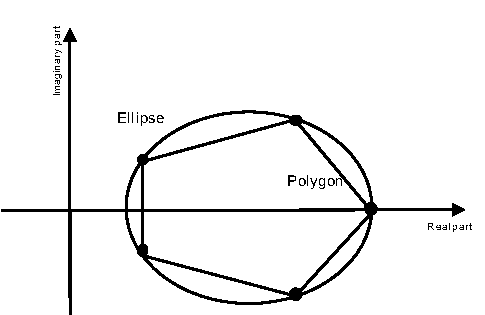
\includegraphics[width=5.4in]{fig/polygon.pdf}
	\caption{The polygon of samllest area containing the convex hull of $\lambda(A)$.}
	\label{polygon}
\end{figure}


\textbf{Weight Function and Gram Matrix}


Suppose that matrix \(A\) is real, we know that its spectrum is symmetric with the real axis, which means we will only need the upper half part \(H^+\) of the convex hull \(H\).

Suppse that \(\partial H^+\) the upper part of boundary \(H\) and \(v=1,\cdots,\mu\) that \(\partial H^+=\cup_{v=1}^\mu E_v\). And then, suppose \(c_v\) and \(d_v\), the center and foscal distance of edge \(E_v\). The inner product of two complex polynomials associated with the weight function \(\omega_v\) on the edge \(E_v\) can be expressed as the expression (11).

\begin{equation}
(p,q)_w=2\Re(\sum_{v=1}^v \int_{E_v}p(\lambda) \overline{q(\lambda)} w_v(\lambda)\mathrm{d}\lambda)
\end{equation}

\begin{equation}
w_v(\lambda)=\frac{2}{\pi}|d_v^2-(\lambda-c_v)^2|^{-\frac{1}{2}}
\end{equation}

The function (12) is the weight function sur one edge \(E_v\) generated by the basis of Chebyshev polynomials (expression 13), which facilite to calculate the inner product.

\begin{equation}
T_i(\frac{\lambda-c_v}{d_v})
\end{equation} 

When we project \(p\) and \(q\) into this basis on the edge \(E_v\), we could get the equations (14) and (15), then the inner product will result into equation (16).

\begin{equation}
p(\lambda)=\sum_{i=0}^n \xi ^v T_i(\frac{\lambda-c_v}{d_v})
\end{equation}

\begin{equation}
q(\lambda)=\sum_{i=0}^n \zeta ^v T_i(\frac{\lambda-c_v}{d_v})
\end{equation}

\begin{equation}
(p,q)_w=2\Re[\sum_{v=1}^\mu 2\xi_0^v \bar{\zeta}_0^v+\sum_{i=1}^\mu 2\xi_1^v \bar{\zeta}_1^v]
\end{equation}

And then, suppose that \(t_j\) the Chebyshev basis on the ellipse \(\xi(c,d,a)\) with \(j \geq 0\), and we can obtain the three terms recurrence with \(i \geq 0\) such as equation (18).

\begin{equation}
t_j(\lambda)=\frac{T_j \frac{\lambda-c}{d}}{T_j \frac{a}{d}}
\end{equation}

\begin{equation}
\beta_{i+1} t_{i+1}(z)=(z-a)t_i(z)-\delta_i t_{i-1}(z)
\end{equation}

With this polynomial basis, we can obtain a so-called modified Gram matrix \(M_n=m_{i,j}\), which is well-conditioned. The entries of \(M_n\) defined by the relation (19) where \(i,j \in 1,\cdots,n+1\), and we can express the inner production formula (16) into the equation (20) with \(\eta=(\eta_1,\cdots,\eta_n)\) and \(\theta=(\theta_1,\cdots,\theta_n)\), which are the coordinates of polynomials \(p\) and \(q\) in basis \(t_i\). 
\begin{equation}
m_{i,j}=(t_{i-1},t_{j-1})_\omega
\end{equation}

\begin{equation}
(p,q)_\omega=(M_n\eta, \theta)
\end{equation}

Expanding the polynomial \(P_n\) into the Chebyshev basis, and then we can get \(R_n\) as equation (22), and in the end we obtain the equation (23) with the three terms recurrence (18). 
\begin{equation}
P_n=\sum_{i=0}^{n-1}\eta_i t_i
\end{equation}

\begin{equation}
\begin{aligned}
R_n(\lambda)&=1-\lambda P_n(\lambda)\\ &=1-\sum_{i=0}^{n-1} \eta_i \lambda t_i(\lambda)
\end{aligned}
\end{equation}

\begin{equation}
\begin{aligned}
R_d(\lambda) =t_0-\sum_{i=0}^{n-1} \eta_i (\beta_{i+1}t_{i+1}+\alpha_i \eta_i + \delta_i \eta_{i+1})t_i.
\end{aligned}
\end{equation}

Then we can can express \(R_n\) into \(e_1-T_n \eta\) with its coordinations in the polynomial \(t_i\), where \(T_n\) is a \((n+1) \times n\) matrix as (24).
\begin{equation}
T_n=
\begin{bmatrix}
\alpha_0       & \delta_1  \\
\beta_1       & \alpha_1 & \delta_2  \\
&  \beta_2 & \alpha_2  & \delta_3\\
& \\
& && &&\delta_{n-1} \\
& && &\beta_{n-1}&\alpha_{n-1} \\
& && &&\beta_{n}
\end{bmatrix}
\end{equation}

With the definition of inner product in the polynomial basis, the function which needs to be minimized can be expressed under the form of equation (25). As \(M_n\) is symmetric, we can get the factorization of \(M_n\) under the form \(M_n=L_n L_n^T\), and in the end we obtain the equation (26) with \(F_n=L_n^TT_k\) a \((n+1) \times n\)upper Hessenberg matrix.
\begin{equation}
\begin{aligned}
||R_n|| &=(R_n,R_n)_\omega \\ &=(M_n(e_1-T_n\eta),e-T_n\eta).
\end{aligned}
\end{equation}

\begin{equation}
\begin{aligned}
||R_n|| &=(R_n,R_n)_\omega \\ &=(L_n^T(e_1-T_n\eta), L_n^T(e_1-T_n\eta)) \\ &=||L_n^T(e_1-T_n\eta)||_2 \\ &=||l_{1,1}-F_n\eta||
\end{aligned}
\end{equation}

The coefficients \(\eta_i\) are the solution of problem \(\min ||l_{1,1}e_1-F_k\eta||_2\) with \(\eta \in IR^n\). This probelm can maybe resolved easily by Givens rotations and QR fatorization. The process to generate the least polynomials by the eigenvalues are given in Algorithm \ref{alg:lsqr-parameters}.

\textbf{Non-Hermitian Linear Systems}

\textcolor{red}{TO DO}

\textbf{Calcul the Iteration Form}

In order to resolve the minimum-maximum problem, a well known method is to use the Chebyshev polynomial, where \(H_k\) is taken to be an ellipse with center \(c\) and focal distance \(d\). This ellipse contains the convex hull of \(\sigma_k(A)\). If the origin is outside of this ellipse, the minimal polynomial can be reduced to a scaled and shifed Chebyshev polynomial:

\begin{equation}
R_d(\lambda)=\frac{T_d(\frac{c-\lambda}{d})}{T_d (\frac{c}{d})}
\end{equation}

The three terms recurrence of Chebyshev polynomial introduces an elegant algorithm for generating the approximation \(x_d\) that uses only three vectors of storage. The choice of ellipses as enclosing regions in Chebyshev acceleration maybe overly restrictive and ineffective if the shape of the convex hull of the unwanted eigenvalues bears little resemblance to an ellipse. There are several reseach to find the acceleration polynomial to minimize its $L_2$-norm on the boundary of the convex hull of the unwanted eigenvalues with respect to some suitable weight function $\omega$. An algorithm based on the modified moments  for computing the least square polynomial was proposed by Youcef Saad (\cite{saad1987least}). The problem tends to find a polynomial \(P_d\) on the boundary of \(H_k\) which we note as \(\partial H_k\), that maxmimizes the modulus of \(|1-\lambda P_d(\lambda)|\). And then we get the least square problem with respect to some weight \(w(\lambda)\) on the boundary of \(H_k\) and the constraint \(R_d(0)=1\).

The iteration form of Least Square is \(x_d=x_0+P_d(A)r_0\) with \(P_d\) the least square polynomial of degree \(d-1\) under the Formula (\ref{pd}). The polynomial basis \(t_i\) meet the three terms recurrence relation (\ref{threeterms}). 
\begin{equation}
\label{pd}
P_d=\sum_{i=0}^{d-1}\eta_it_i.
\end{equation}

\begin{equation}
\label{threeterms}
t_{i+1}(\lambda)=\frac{1}{\beta i+1}[\lambda t_i(\lambda)-\alpha_i t_i(\lambda)-\delta_i t_{i-1}]
\end{equation}

For the computation of parameters $H=(\eta_0,\eta_1,\cdots,\eta_{d-1})$, we construct a modified gram matrix $M_d$ with dimension $d \times d$, and matrix $T_d$ with dimension $(d+1) \times d$ by the three terms recurrence of the basis $t_i$. $M_d$ can be factorized to be $M_d=LL^T$ by the Cholesky factorization. The parameters $H$ can be computed by a least squares problem of the formula


\begin{equation}
\label{eq112}
min \|l_{11}e_1-F_d H\|
\end{equation}

We therefore need to compute the vectors \(\omega_i=t_i(A)r_0\), and get the linear combination of formula (\ref{pd}). The recurrence expression of $ \omega_i$ is given as (\ref{omegai}) and the final solution value as (\ref{xd}). The hybrid GMRES preconditioned by least squares polynomial methods is given as Algorithm \ref{alg:hybrid-gmres-ls}.

\begin{equation}
\label{omegai}
\omega_{i+1}=\frac{1}{\beta_{i+1}}(A\omega_i-\alpha_i\omega_i-\delta_i\omega_{i-1})
\end{equation}

\begin{equation}
\begin{aligned}
\label{xd}
x_d &=x_0+P_d(A)r_0 \\ &=x_0+\sum_{i=1}^{d-1}\eta_i\omega_i.
\end{aligned}
\end{equation}

\begin{algorithm}[htbp]
	\caption{Least Square Polynomial Generation}
	\label{alg:lsqr-parameters}
	\begin{algorithmic}[1]
		\Function {LSP}{$input$: $A,b,d,\Lambda_r$, $output$: $A_d, B_d, \Delta_d, H$}
		\State construct the convex hull $C$ by $\Lambda_r$
		\State construct $ellispe(a,c,d)$ by the convex hull $C$
		\State compute parameters $A_d, B_d, \Delta_d$ by $ellispe(a,c,d)$
		\State construct matrix $T$ ${(d+1)} \times d$ matrix by $A_d, B_d, \Delta_d$
		\State construct Gram matrix $M_d$ by Chebyshev polynomials basis
		\State Cholesky factorization $M_d=LL^T$
		\State $F_d=L^TT$
		\State $H_d$ satisfies min $\|l_{11}e_1-F_d H\|$
		\EndFunction
	\end{algorithmic}
\end{algorithm}

\begin{algorithm}[htbp]
	\caption{Hybrid GMRES Preconditioned by Least Squares Polynomial}
	\label{alg:hybrid-gmres-ls}
	\begin{algorithmic}[1]
		\State  Compute current residual vector $r=b-Ax$
		\State Run $m_1$ steps of GMRES for solving $Ad = r$.
		\State  Update $x$ by $x=x+d$.
		\State  Get eigenvalue estimates from the eigenvalues $\Lambda_r$ of the Hessenberg matrix.
		\State  LSP($input$: $A,b,d,\Lambda_r$, $output$: $A_d, B_d, \Delta_d, H$)
		\State  $r_0=f-Ax_0$, $\omega_1 = r_0$ and $x_0=0$
		\For  {$k=1,2,\cdots, s_{use}$}
		\For  {$i=1, 2, \cdots, d-1$}
		\State  $\omega_{i+1}=\frac{1}{\beta_{i+1}}[A\omega_i-\alpha_i\omega_i-\delta_i\omega_{i-1}]$
		\State  $x_{i+1}=x_i+\eta_{i+1}\omega_{i+1}$
		\EndFor
		\EndFor
		\State  set $x_0=x_d$
		\State  Test for convergence.
		\State  If solution converged then Step, else GoTo 1.
	\end{algorithmic}
\end{algorithm}


\section{GMRES Convergence Analysis}

Many things have been proposed over the years to explain GMRES convergence:

\begin{itemize}
	\item Eiegenvalues of $A$;
	\item Pseudo-eigenvalues;
	\item Polynomial numerical hull.
\end{itemize}

This section summarize these discussions.
 
\subsection{Convergence Analysis by Eigenvalues}

\textcolor{red}{TO DO}

G\'erard MEURANT completely describes GMRES convergence for normal matrices. Convergence depends on the eigenvalues of $A$ and on its eigenvectors and $b$ through the weights. 

When $A$ is normal, GMRES convergence depends on the eigenvalues and eigenvectors of $A$. 

\textcolor{red}{TO DO}

GMRES convergence is governed by the distribution of the eigenvalues of $V^TW$ on the unit circle (and also the weights $\omega_i$).  When $A$ is non-normal, GMRES convergence depends on the eigenvalues and eigenvectors of $Q=V^TW$.

\begin{theorem}
	Denote $x_m$ be the approximate solution obtained from the $m$-th step of GMRES, and the related residual is $r_m=b-Ax_m$. Then, $x_m$ is of the form:
	
	\begin{equation}
		x_m = x_0 + q_m(A)r_0
	\end{equation}
	
	and 
	\begin{equation}
		||r_m||_2=||(I-Aq_m(A))r_0||_2=\min_{q \in \mathbb{P}_{m-1}}||(I-Aq(A))r_0||_2
	\end{equation}
\end{theorem}

\begin{theorem}
	If $A$ is a $n \times n$ diagonalizable matrix and let $A=P\Lambda P^{-1}$ with $\Lambda=diag{\lambda_1, \lambda_2, \cdots, \lambda_n}$ is the diagonal matrix of eigenvalues. Then the residual norm achieved by the $m$-th step of GMRES satisfies the inequality
	
	\begin{equation}
		||r_m||_2 \leq c_2(P)\epsilon^{(m)}||r_0||_2.
	\end{equation}
\end{theorem}

where $\epsilon^{(m)}=\min_{p \in \mathbb{P}_m, p(0)=1} \max_{\lambda \in \sigma(A)i=1,\cdots,n}|p(\lambda_i)|$, and $c_2(P)=||P||_2||P^{-1}||_2$.

The exact proof can be found in (\cite{saad2003iterative}).

\subsection{Convergence Analysis by Pseudo-eigenvalues}

\subsection{Convergence Analysis by Polynomial Numerical Hull}


\begin{corollary}
	If $A$ is a $n \times n$ diagonalizable matrix and let $A=P\Lambda P^{-1}$ with $\Lambda=diag{\lambda_1, \lambda_2, \cdots, \lambda_n}$ is the diagonal matrix of eigenvalues. Assume that all the eigenvalues of $A$ are located in the ellipse $E(c,d,a)$ which excludes the origin. The residual norm achieved at the $m$-th step of GMRES satisfies the inequality.
	
	\begin{equation}
	||r_m||_2 \leq c_2(P)\frac{C_m(\frac{a}{d})}{|C_m\frac{c}{d}|}||r_0||_2.
	\end{equation}
\end{corollary}

\section{Parallel Krylov methods on Large-scale Supercomputers}

Krylov subspace methods are generally implemented in parallel on the supercomputers to solve very large linear systems and eigenvalue problems. This section discusses the scheme to implement Krylov methods in parallel.

\subsection{Core Operations in Krylov Methods}

It is necessary to identify the main operations in Krylov methods before the parallel implementation. Consider Algorithm \ref{alg:arnoldi-reduction}, \ref{alg:basicgmres} and \ref{alg:arnoldi}. We distinguish four types of operations, which are:

\begin{itemize}
	\item Matrix-vector products in step $5$ of Algorithm \ref{alg:arnoldi-reduction};
	\item AXPY operation in step $7$ of Algorithm \ref{alg:arnoldi-reduction};
	\item Dot products in step $8$ of Algorithm \ref{alg:arnoldi-reduction};
	\item Orthogonalization of vector for the loop from step $4$ to $6$ in of Algorithm \ref{alg:arnoldi-reduction}.
\end{itemize}

This section gives the parallel implementation of these four operations in details.

\subsubsection{AXPY Operation}

AXPY is in the form:

\begin{equation}
y = \alpha x + y.
\end{equation}

With $x$ and $y$ two vectors, and $\alpha$ is a scalar. This operation is used to \textit{update vectors} inside Krylov subspace methods. On distributed memory platforms, it is necessary to assume that the vectors $x$ and $y$ should be distributed in the same manner across all the processor. The distributed AXPY is simple without requiring communication. It can be regarded as several AXPY of local vectors in serial on each processor.

\subsubsection{Dot product and Global Reduction Operation}

The dot product is the operation that use all the components of given vectors to compute a single floating-point scalar. In the Arnoldi reduction process, this scalar is always needed by all processors. Equation (\ref{dotproduct}) gives the formula of dot product operation.

\begin{equation}
\label{dotproduct}
v\cdot w = \langle v_1, v_2, \cdots, v_n \rangle \cdot\langle w_1, w_2, \cdots, w_n\rangle = v_1w_1+v_2w_2+\cdots+v_nw_n.
\end{equation}
The distributed version of the dot-product is needed to compute the inner product of two vectors $v$ and $w$ and then distribute the result across all the processors.  This types of operations are termed the \textit{All Reduction Operations}, which can be seen as the combination \textit{Reduction Operations} and \textit{Broadcast Operations}. In Krylov subspace methods, the dot-product operation is typically needed to perform the vector update on each processor. If the number of processors is large, this kind of operations can introduce enormous communication costs. The computation of the Euclidean norm of distributed vectors is also a global reduction operation which is similar to the dot-product.

\subsubsection{Orthogonalization of Vector}

In the Arnoldi reduction (as shown by Algorithm \ref{alg:arnoldi-reduction}) for non-Hermitian matrices, the vector $Av_i$ should be orthogonalized against all the previous vectors. In practice, the classic Gram-Schmidt process is preferred than the Modified Gram-Schmidt, even the presence of round-offs and cancellations within CGS diminish its numerical stability. In CGS, the orthogonalization process is overlapped, while the same process of MGS has a data dependency, which is not possible to get good parallel performance. A preconditioner or a reorthogonalization process can compensate the deficiency of numerical stability.

\begin{figure}[h]
	\centering
	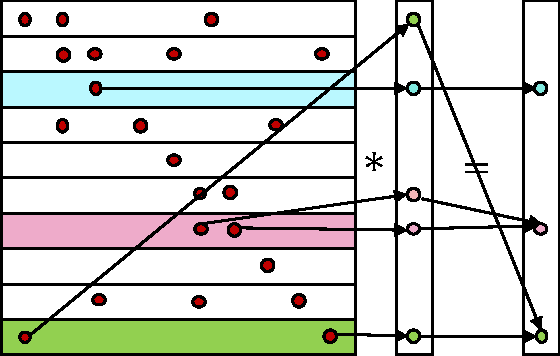
\includegraphics[width=4.8in]{fig/spmv.pdf}
	\caption{Communication Scheme of SpMV.}
	\label{fig:spmv}
\end{figure}

\subsubsection{Matrix-vector products}

In practice, the parallel version of Arnoldi orthogonalization is memory/communication bounded. The most critical operation with the high communication intensity is the substantial number of matrix-vector multiplications $Av_i$. Krylov subspaces are often used to solve linear systems and eigenvalue problems associated with the sparse matrix. Its parallel implementation depends heavily on the data structure to store the matrix. Different distributed sparse matrix format introduces different matrix-vector implementation scheme and finally results in the different parallel performances.

The standard used sparse matrix storage format includes: COO (Coordinate lists) which stores respectively the row index, column index and values into three arrays; CSR (Compressed Sparse Row) which stores respectively the row offset, the column index and data values into three arrays; ELLPACK which stores the column index and values into two two-dimensional arrays according their row index; and DIA (Diagonal format) which store the diagonal offsets into one-dimensional array, and the values sorted by diagonal into a two-dimensional array.

For the parallel implementation of SpMV on modern parallel systems, the matrix with selected storage format should be distributed across different processors with considering the load balance and reduction of communications. Fig. \ref{fig:spmv} gives the communication scheme of SpMV on distributed memory memory systems.

\begin{figure}[h]
	\centering
	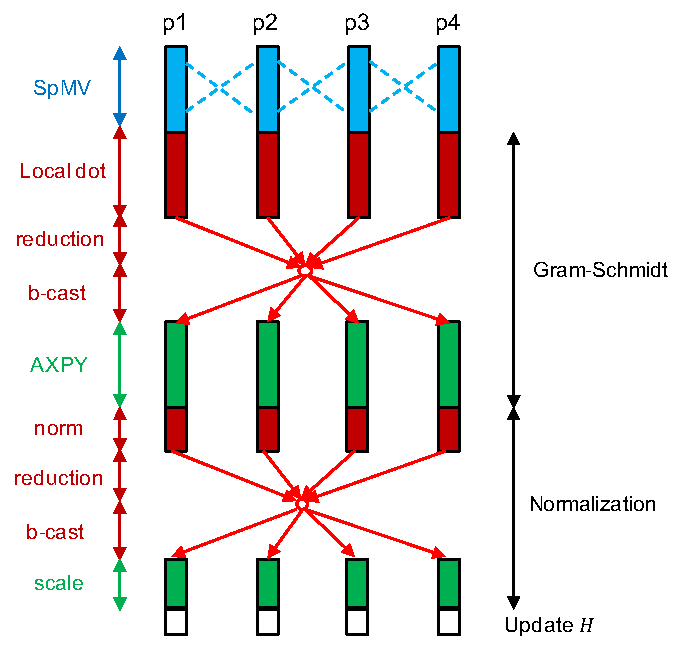
\includegraphics[width=5.4in]{fig/parallel_gmres.pdf}
	\caption{Classic Parallel implementation of Arnoldi reduction.}
	\label{parallel_gmres}
\end{figure}

\subsubsection{Parallel GMRES on Distributed Memory Systems}

Fig. \ref{parallel_gmres} describes the parallel implementation of the Arnoldi reduction process inside GMRES.  For each loop inside, it can be divided into two parts: the Gram-Schmidt and the normalization processes. The SpMV in Gram-Schmidt process is implemented in parallel with the communication among the processors, and the distributed version of dot-product operation is the combination of \textit{Reduction} and \textit{Broadcast} Operations, which introduce a synchronization point, and the AXPY is implemented in parallel without communications. In the normalization process, the computation of the norm of the distributed vectors also introduce the synchronization points. In the Arnoldi reduction, this loop is executed in sequence for $m$ times to generate an orthonormal basis in the $m$-dimensional Krylov subspace.

\subsection{Existing Softwares}

Recent years, there are several efforts to provide the parallel Krylov methods on different computing architectures. This section gives a glance at two famous ones of them.

\subsubsection{PETSc/SLEPc} 

The \textbf{Portable, Extensible Toolkit for Scientific Computation (PETSc)} (\cite{balay2001petsc}), is a suite of data structures and routines developed by Argonne National Laboratory for the scalable (parallel) solution of scientific applications modeled by partial differential equations. It employs the Message Passing Interface (MPI) standard for all message-passing communication. PETSc provides many of the mechanisms needed within parallel application code, such as simple parallel matrix and vector assembly routines that allow the overlap of communication and computation. PETSc provides the parallel implementation of Krylov methods and several preconditioners.

The \textbf{Scalable Library for Eigenvalue Problem Computations (SLEPc)} (\cite{hernandez2005slepc}) is a software library for the parallel computation of eigenvalues and eigenvectors of large, sparse matrices. It can be seen as a module of PETSc that provides solvers for different types of eigenproblems, including linear (standard and generalized) and nonlinear (quadratic, polynomial and general), as well as the SVD. Recent versions also include support for matrix functions. It uses also the MPI standard for parallelization. Both real and complex arithmetic are supported, with single, double and quadruple precision. When using SLEPc, the application programmer can use any of the PETSc's data structures and solvers. Other PETSc features are incorporated into SLEPc as well. The module \textit{EPS} in SLEPc provides Krylov subspace methods such as Krylov-Schur, Arnoldi and Lanczos to solve sparse eigenvalue problems.

\subsubsection{Trilinos} 

\textbf{Trilinos} (\cite{heroux2005overview}) is a collection of open-source software libraries, intended to be used as building blocks for the development of scientific applications. The word "Trilinos" is Greek and conveys the idea of "a string of pearls," suggesting a number of software packages linked together by a common infrastructure. Trilinos was developed at Sandia National Laboratories from a core group of existing algorithms and utilizes the functionality of software interfaces such as the BLAS, LAPACK, and MPI (the message-passing interface for distributed-memory parallel programming). Fortunately, Trilinos supports many different packages which are defined to implement the iterative linear and eigen-solvers methods. There are some packages which are widely used as follows:

\begin{itemize}
	\item \textbf{Kokkos (\cite{edwards2014kokkos})}: Kokkos Core implements a programming model in C++ for writing performance portable applications targeting all major HPC platforms. For that purpose, it provides abstractions for both parallel executions of code and data management. Kokkos is designed to target complex node architectures with N-level memory hierarchies and multiple types of execution resources. It currently can use OpenMP, Pthreads, and CUDA as backend programming models.
	\item \textbf{Epetra (\cite{heroux2005epetra})}: Epetra provides the fundamental construction routines and services function that are required for serial and parallel linear algebra libraries. Epetra provides the underlying foundation for all Trilinos solvers.
	
	\item \textbf{Tpetra (\cite{baker2012tpetra})}: Tpetra is the next version of Epetra with better support for shared-memory parallelism. It implements linear algebra objects including sparse graphs, sparse matrices, and dense vectors.  Many Trilinos packages and applications produce, modify, or consume Tpetra’s linear algebra objects, or depend on Tpetra’s parallel data redistribution facilities. Tpetra is “hybrid parallel,” meaning that it uses at least two levels of parallelism: MPI  for distributed-memory parallelism and Any of various shared-memory parallel programming models within an MPI process, Tpetra uses the Kokkos package’s shared-memory parallel programming model for data structures and computational kernels.  Kokkos makes it easy to port Tpetra to new computer architectures and to extend its use of parallel computational kernels and thread-scalable data structures.  Kokkos supports several different parallel programming models, including OpenMP, POSIX Threads and Nvidia’s CUDA programming model for graphics processing units (GPUs). Tpetra has the following unique features:
	
	\begin{itemize}
		\item Native support for representing and solving very large graphs, matrices, and vectors.  “Very large” means over two billion unknowns or other entities;
		\item Matrices and vectors may contain many different kinds of data, such as floating-point types of different precision and complex-valued types;
		\item Support for many different shared-memory parallel programming models based on Kokkos.
	\end{itemize}
	
	\item \textbf{AztecOO (\cite{heroux2004aztecoo})}: Preconditioners and Krylov subspace methods (conjugate gradient, GMRES, etc.), compatible with Epetra only.
	\item \textbf{Belos (\cite{bavier2012amesos2})}: Classical and block Krylov subspace methods (implementations of iterated classical Gram-Schmidt (ICGS), classical Gram-Schmidt with a DGKS correction step, implementations of conjugate gradient (CG), block CG, block GMRES, pseudo-block GMRES, block flexible GMRES, and GCRO-DR iterations). Belos is compatible with Epetra and Tpetra.
	\item \textbf{Anasazi (\cite{baker2009anasazi})}: Parallel eigensolvers, Anasazi is compatible with Epetra and Tpetra. It is a package within the Trilinos Project that uses ANSI C++ and modern software paradigms to implement algorithms for the numerical solution of large-scale eigenvalue problems.
	\item \textbf{Komplex (\cite{day2001solving})}: Complex-valued system solver, KOMPLEX is an add-on module to AztecOO that allows users to solve complex-valued linear systems. KOMPLEX solves a complex-valued linear system Ax=b by solving an equivalent real-valued system of twice the dimension.
\end{itemize}

\section{Toward Extreme Computing, Some Correlated Goals}
%Global vs Local Communication, fault tolerance, multiple level parallellism, etc. 

This section gives the challenges of numerical methods facing the development of HPC platforms. In Section \ref{Exascale Challenges of Supercomputers}, we discussed the tendance of future exascale supercomputing architectures and the related challenges of parallel programming to develop the applications to profit efficiently from these supercomputers. The main objective for the parallel implementation of numerical methods is to minimize the global computing time. The global computing time of an algorithm can be reduced by either accelerating the convergence or improve its parallel scaling performance using much more computing units. In section, we list in details the correlated goals of iterative methods toward the extreme computing below:

\begin{enumerate}
	
	\item \textbf{Accelerate the convergence}: When solving linear systems by Krylov subspace, the convergence cannot be guranteed for the ill-conditioned matrix or the restart strategy all used. Thus, one important issue for the iterative methods is to propose different kinds of preconditioners which have better speedup on the convergence, and also enough numerical stability. Moverover, facing the comping exascale computing, the proposed preconditioners should either with better parallel performance across large number of cores, or be able to promote the asynchronisity, and benefit from the more complex architectures of mordern supercomputers. 
	
	\item \textbf{Minimize the number of communications}: When solving very large problems on parallel architectures, the most significant concern becomes the cost per iteration of the method -- typically because of communication and synchronization overheads. In general, the complexity of algorithms (number of operations performed) is used to express their performance rather than the quantity of data movement and communications. In fact, on the exascale computers, the global communications accross millinos of cores are very expensive and the computing operations inside each core will be nearly free. To address the critical issue of communication costs, researchers need to investigate algorithms that minimize communication. Considering inside the Krylov iterative methods such as such as GMRES, CG, and Lanczos, the operations of loop inside Arnoldi reduction much more global communications. 
	
	When matrix $A$ in Krylov subspace methods is very sparse, the sparse matrix-vector multiplication (SpMV) invokes even more communications. Hence, strategies for reducing communication overheads in Arnoldi orthogonalization have been proposed to address this bottleneck. In order to reduce the global communication of SpMV for sparse matrices, the first approach is to select the best sparse matrix storage format, which can produces less communications (e.g. \cite{montagne2004optimal, liu2015csr5,stathis2003hierarchical,merrill2016merge,bell2008efficient, bell2009implementing,kreutzer2014unified,ashari2014efficient}). Another approach is to use the Hypergraph Partitioning Models to optimize the SpMV scheme on parallel computers, e.g. in 1999, Catalyurek et al. proposed two computational hypergraph models which avoid this crucial deficiency of the graph model for SpMV (\cite{catalyurek1999hypergraph}); Vastenhouw et al. tried to reduce the communication volume of SpMV through a recursive bipartitioning of the sparse matrix (\cite{vastenhouw2005two}); Chen et al. proposed a communication optimization scheme based on the hypergraph for basis computation of krylov subspace methods on multi-GPUs (\cite{chen2014communication}); a Locality-aware parallel sparse matrix-vector and matrix-transpose-vector multiplication on many-core processors is introduced by Karsavuran et al. (\cite{karsavuran2016locality}); and spatiotemporal graph and hypergraph partitioning models for SpMV on manycore architectures is presented by Abubaker et al. with better scaling performance through enhancing data locality in the operations \cite{abubaker2018spatiotemporal}, etc.
	
	\item \textbf{Promote the asynchronisity and reduce the synchronization}: One alogrithm often must do the synchronize operations during the computation. The global data synchronization across amount of cores in the distributed memory systems is expensive especially for a hybrid platform with accelerators. Inside Krylov subspace methods, dot product is a good example which needs the global synchronization after its \textit{global reduction}. For the extreme-scale platforms, synchronizations become bottlenecks. Hence, the algorithm should be designed with as few synchronization points as possible.
	
	Attempts have been made to restructure existing algorithms for the exascale computing so that the number of synchronizations is reduced. Communication-avoiding and pipelined variants of Krylov solvers are critical for the scalability of linear system solvers on future exascale architectures. Firstly, the impact of global communication latency at extreme scales on Krylov methods are analyzed by Ashby et al. (\cite{ashby2012impact}). The strategy of hiding global synchronization latency in GMRES and the preconditioned CG was presented by Ghysels (\cite{ghysels2013hiding,ghysels2014hiding}); Fujino et al. evaluated performance of parallel computing of revised BiCGSafe and BiCGStar-plus method, and made clear that the revised single synchronized BiCGSafe method outperforms other methods from the view points of elapsed time and speedup on parallel computer with distributed memory (\cite{fujino2015estimation}); Rupp et al. implemented pipelined iterative solvers with kernel fusion for GPUs \cite{rupp2016pipelined}; Sanan et al. presented variants of CG, CR, GMRES which both piplined and flexible (\cite{sanan2016pipelined}); Yamazaki et al. proposed to improving the performance of GMRES by reducing communication and pipelining global collectives (\cite{yamazaki2017improving}); Swirydowicz et al. presented low synchronization variants of iterated classical (CGS) and modified Gram-Schmidt (MGS) algorithms that require one and two global reduction communication steps; the reduction operations are overlapped with computations and pipelined to optimize performance (\cite{swirydowicz2018low}), etc. Moreover, on important considerationin for the restructuring an algorithm to reduce synchronization and communication is their numerical stability.
	
	\item \textbf{Memory and cache optimization for the heterogeneity and scale}: Extracting the desired performance from environments that offer massive parallelism, especially where additional constraints (e.g., limits on memory bandwidth and energy) are in play, requires more sophisticated scheduling and memory management techniques than have heretofore been applied to linear algebra libraries. Confronting the limits of domain-decomposition in the face of massive, explicit parallelism introduces another form of heterogeneity. Feed-forward pipeline parallelism can be used to extract additional parallelism without forcing additional domain-decomposition, but it exposes the user to dataflow hazards. Ideas relating to a data-flow-like model, where parallelism is expressed explicitly in DAGs, allows for dynamic scheduling of tasks, support of massive parallelism, and application of common optimization techniques to increase throughput. Approaches for isolating side-effects include explicit approaches that annotate the input arguments to explicitly identify their scope of reference and implicit methods, such as using language semantics or strongly typed elements to render code easier to analyze for side-effects by compiler technology. New primitives for memory management techniques are needed that enable diverse memory management systems to be managed efficiently and in coordination with the execution schedule.
	
	\item \textbf{Mixed arithmetic}: One important for the development of numerical methods for the exascale computing is to recognize and exploit the presence of mixed-precision mathematics. Low-precision floating-point arithmetic is a powerful tool for accelerating scientific computing applications, especially those in artificial intelligence. In fact, on the modern computing architectures, the 32-bits operation can achieve at least two times speedup over the performance of 64-bits operations. Additionaly, through the combination of 32-bits and 64-bits floating-point arithmetic, where the performance of many linear algebra algorithms can be significantly enhanced by the 32-bits precision operations while maintaining the 64-bit accuracy of the resulting solution. The mixed archmetic can be applied to the different computing architectures including the conventional CPUs and the accelerators such as GPUs. The creation of mixed-precision algorithms allows more effectively utilizing of the heterogeneous hardwares. Little modification of exsiting codes can provide signficant speedup by taking into account existing hardware properties. 
	
	In 2014, Kouya et al. (\cite{kouya2014highly}), evaluate the performance of Krylov subspace methods by using highly efficient multiple precision SpMV. They show that SpMV implemented in these functions can be more efficient. (\cite{yamazaki2015mixed}), Yamazaki present a mixed-precision Cholesky factorization, which has $1.4\times$ speedup over the standard approach on GPU. Additionaly, their studies of  using the mixed-precision Cholesky factorization within communication-avoiding variants of Krylov subspace projectionmethods demonstrate that by using the higher precision for this small but critical segment of the Krylov methods, we can improve not only the overall numerical stability of the solvers but also, in some cases, their performance. In 2018, Haidar et al. (\cite{haidar2018harnessing}) investigate how HPC applications can be accelerated by the mixed arithmetic technique. In details, they developed the architecture-specific algorithms and highly tuned implementations of a solver based on mixed-precision (FP16-FP64) iterative refinement for the general linear system, $Ax=b$, where $A$ is a large dense matrix, and a double precision (FP64) solution is needed for accuracy. Their paper show how using half-precision Tensor Cores (FP16-TC) for the arithmetic can provide up to $4\times$ speedup. Maynard et al.  (\cite{maynard2018precision}) present a mixed-precision implementation of Krylov solver for the numerical weather prediction and climate modelling, the beneficial effect on run-time and the impact on solver convergence. The complex interplay of errors arising from accumulated round-off in floating-point arithmetic and other numerical effects is discussed. They employ now the mixed-precision solver in the operational forecast to satisfy run-time constraints without compromising the accuracy of the solution.
	
	\item \textbf{Minimize energy consumption}: The generated heat also affects the performance of clusters such as the arising failure rate of hardware, and the energy consumption also becomes a tremendous financial burden for supercomputer centers, because it takes up a large portion in the total cost of ownership (TCO), that is the \textit{Power wall}, another roadrock to approach the exascale computing. The HPC community starts to address this problem in recent years, and it is necessary to build power and energy awareness, control, and efficiency of numerical methods and libraries. 
	
	In 2013, an analysis of energy-optimized lattice-Boltzmann CFD simulations from the chip to the highly parallel level is introduced by Wittmann et al. (\cite{wittmann2013analysis}). Padoin et al. (\cite{padoin2013evaluating}) evaluated the application performance and energy consumption on hybrid CPU+ GPU architecture. In 2015, Anzt et al. (\cite{anzt2015energy}) unveil some energy efficiency and performance frontiers for sparse computations on GPU-based supercomputers. Aliaga et al. (\cite{aliaga2015unveiling}) unveil the performance-energy trade-off in iterative linear system solvers for multithreaded processors. In order to gain insights about the benefits of hands-on optimizations, they analyze the runtime and energy efficiency results for both out-of-the-box usage relying exclusively on compiler optimizations, and implementations manually optimized for target architectures,that range from CPUs and DSPs to manycore GPUs.
	
	\item \textbf{Multi-level Parallelism}: 
	
	\item \textbf{Adaptive response to load imbalance}: For the exascale computing with millinons of cores and accelerators, even naturally load-balanced algorithms on homogeneous hardware will present many of the same load-balancing problems. Dynamic scheduling based on directed acyclic graphs (DAGs) has been identified as a path forward, but this approach will require new approaches to optimize for resource utilization without compromising spatial locality. The current implementation DAGs based runtime including StarPU (\cite{augonnet2011starpu}), OmpSs (\cite{duran2011ompss}), etc.
	
	\item \textbf{Autotuning}: Numerical algorithms and libraries need the ability to adapt to the possibly heterogeneous environment in which they operate. Such adaptation must deal with the complexity of discovering and applying the best algorithm for diverse and rapidly evolving ar- chitectures. An automated process would be best, both for productivity and for correctness, where productivity refers both to the development time of the implementation and to the user’s time to solution. The objective is to provide a consistent library interface that, independent of scale and processor heterogeneity, can achieve good performance and efficiency by binding to different under- lying code, depending on the configuration. The diversity and rapid evolution of today’s platforms mean that autotuning of libraries such as the BLAS will be indispensable to achieving good perfor- mance, energy efficiency, and load balancing across the range of systems. In addition, autotuning has to be extended to frameworks that go beyond libraries, such as optimizing data layout (e.g., blocking strategies for sparse matrix/SpMV kernels), stencil autotuners (since stencils kernels are diverse and not amenable to library calls), and even tuning of the optimization strategy for multigrid solvers (optimizing the transition between the multigrid coarsening cycle and bottom-solver to minimize runtime). Adding heuristic search techniques and combining these with traditional compiler techniques will enhance the ability to address generic problems extending beyond linear algebra.
	
	Aquilanti et al. (\cite{aquilanti2011parallel}) present a general parallel auto-tuned linear solver approach based on the tuning of the Arnoldi incomplete orthogonalization process within GMRES by monitoring the convergence in order to reduce the time of computation needed for a solver to attain solution. Katagiri et al. (\cite{katagiri2012smart}) presented a smart tuning strategy for restart frequency of GMRES with hierarchical cache sizes.
	
	\item \textbf{Fault tolerance, resilience}: Computing an incorrect answer quickly is of no use to a scientist. Yet computing with exascale hardware poses several challenges in assessing and assuring the correctness of numerical simulation results. Resilience to faults has been identified as a critical need for future HPC systems [57]; the thousandfold increase in computational capabilities expected over the next decade, along with incorporation of techniques for reducing energy consumption, is predicted to increase the error rate of the largest systems. DOE has several critical mission deliverables, including annual stockpile certification and safety assurance for the NNSA and future energy generation technologies for the Office of Science. Computer simulations are key to meeting these deliverables and must be resilient enough to complete in time and correctly, in order to meet the respective critical mission need. In many cases, these simulations can take days, weeks, or even months to complete, which increases the computation’s exposure to faults. Both hard and soft faults are expected to occur with much greater frequency than on previous hardware. Uncorrected soft faults have the potential to corrupt computed solutions. Hard faults will need to be handled on the fly; halting and restarting an entire application because of the loss of a node, for instance, will be prohibitively expensive at the exascale. Dynamically recovering from either type of fault will introduce nondeterministic variability in resource usage, as will dynamic scheduling of tasks. Because of the nonassociativity of floating-point arithmetic, such nondetermin- ism will make bitwise reproducibility difficult at best and will complicate code correctness testing procedures, including code verification, where reproducible execution behavior is assumed. Preventing all faults during exascale simulation will be impossible, and nondeterministic execu- tion is likewise unavoidable without potentially severe performance penalties. Fault management will require developments in hardware, programming environments, runtime systems, and pro- gramming models; but mathematics will play an important role as well. The issue of correctness is ultimately a mathematical one and will require mathematics-informed solutions. Research will be required in order to devise efficient application-level fault-tolerance mechanisms and new procedures to verify code correctness at scale.

\end{enumerate}

The work of this dessertition try to propose a potential smart multi-level parallel programming with auto-tuning scheme for solving linear systems which address on the goals of acceleration of convergence, minimizing the number of communications, promoting the asynchronisity, reducing the synchronize points and fault tolerance.

\clearemptydoublepage

\chapter{Sparse Matrix Generator with Given Spectra}\label{Sparse Matrix Generator with Given Spectra}

\begin{displayquote}
	\textsf{In Chapter 3, we have discussed the convergence of iterative methods and its relation with spectral distribution of linear systems. Indeed, algorithms and applications from diverse fields can be formulated as an eigenvalue problem. The eigenvalues are also extremely important for the preconditioners of solving linear systems. In machine learning and pattern recognition, it is often demanded to solve the eigenvalue problems for both supervised and unsupervised learning algorithms, such as principal component analysis (PCA) \cite{croux2000principal}, Fisher discriminant analysis (FDA) \cite{berkes2005handwritten}, and clustering \cite{fender2017parallel}, etc. An insufficient accuracy and a failure of eigenvalue solvers and linear solvers usually result in, respectively, a poor approximation to original discrete problems and a failure of entire algorithms.  A good selection of solvers becomes especially essential. Thus it is crucial to have the test matrices to benchmark the numerical performance and parallel efficiency of different methods. In this section, we present the Scalable Matrix Generator with Given Spectra (SMG2S), including its parallel implementation and optimization of both CPU and GPU clusters, the verification mechanism, and the release of open source package.}
\end{displayquote}

\vspace{0.6in}

\section{Demand of Large Matrices with Given Spectrum}

As presented in Chapter 3, nowadays, the size of eigenvalue problems and the supercomputer systems continue to scale up. The whole ecosystem of High-Performance Computing (HPC), especially the linear system applications, should be adjusted to this kind of large clusters. Under this background, there are four special requirements on the test matrices for the evaluation of numerical algorithms on extreme-scale platforms: 

\begin{enumerate}
	\item their spectra must be known and can be customized;
	\item they should be both sparse, non-Hermitian and non-trivial;
	\item they could have a very high dimension, including the non-zero element numbers and/or the matrix dimension, to evaluate the numerical algorithms on large-scale systems, which means that the proposed matrix generator should be able to be parallelized to profit from the large distributed memory clusters.
	\item their sparsity patterns should be controllable.
\end{enumerate}

In order to provide numerically robust solvers of eigenvalue or linear system problems, the researchers need the matrices whose spectra are known, which help to analyze the numerical accuracy. Some scientific communities may be interested in matrices with clustered, conjugated eigenvalues, the closest eigenvalues in random distribution or contained in a specified interval. It is significant to develop a suite of very large Non-Hermitian test matrices whose eigenvalues can be given.

The properties of being sparse, non-Hermitian and non-trivial together can add many mathematical features to simulate the matrices in reality. Besides, the test matrices should have very high dimensions for the experiments on large-scale platforms. This means that the proposed generation method should be easily parallelized to exploit the modern cluster platforms. Furthermore, since the enormous matrix is generated in a parallel way, its different slices are already distributed on separate computing units, which can be directly used to evaluate the required linear and eigenvalue solvers, without concerning loading the large matrix file from the filesystems. It can save time and improve the efficiency for the applications.

In this chapter, we present a Scalable Matrix Generator from Given Spectra (SMG2S) for testing the linear and eigenvalue solvers on large-scale platforms. In Section \ref{Existing Collections}, we introduce the related work to propose test matrix collections. In Section 4.3, we give the proof of mathematical framework of SMG2S to generate matrices with given spectra. In Section 4.4, the numerical algorithm and practical implementation of SMG2S are presented. In section 4.5, firstly, we give a naive implementation of SMG2S based on PETSc\footnote{Portable, Extensible Toolkit for Scientific Computation.} for homogenous platforms and PETSc+CUDA\footnote{Compute Unified Device Architecture} for heterogeneous machines with multi-GPU. Then an open source package\footnote{https://github.com/smg2s/SMG2S} with specific communication optimization based on MPI\footnote{Message Passing Interface.} and C++ is available.  In Section 4.6, the evaluations of its scalability and the accuracy to keep the given spectra are presented on different supercomputing platforms.  A mechanism to verify the capacity of the generated matrix to keep the given spectra has been proposed based on the Shifted Inverse Power Method in Section 4.7, and the accuracy verification for various spectral distribution is also presented in this section. In Section 4.8, we introduce the SMG2S package as a released software, including the interfaces to different programming languages and scientific computational libraries, the Graphic User Interface (GUI) for verification, and also an example to evaluate the Krylov solvers. 

\section{The Existing Collections} \label{Existing Collections}

It's rare but there are already several efforts to supply test matrix collections for linear problems. SPARSEKIT \cite{saad1994sparsekit} implemented by Y. Saad contains various simple matrix generation subroutines. Z. Bai et al. \cite{bai1996test} presented a collection of test matrices for the development of numerical algorithms for solving nonsymmetric eigenvalue problems. There are also two widely spread matrix providers, the Tim Davis collection \cite{davis2011university} and Matrix Market \cite{boisvert1997matrix}. They all contain many matrices with various mathematical properties coming from different scientific fields. However, the spectra of matrices in these collections are fixed, and that cannot be whatever we want. A test matrix generation suite with given spectra was already introduced by J. Demmel et al. \cite{demmel1989test} in 1989 for the benchmark of LAPACK\footnote{Linear Algebra PACKage}. They proposed the method to transfer the diagonal matrix with given spectra into a dense matrix with same spectra using the orthogonal matrices, and then reduce them to unsymmetric band ones by the Householder transformation. This method requires $\mathcal{O}(n^3)$ time and $\mathcal{O}(n^2)$ storage even for generating a small bandwidth matrix. Moreover, this method was implemented for the shared memory systems, not for larger distributed memory systems, thus it is difficult to generate large-scale test matrices customized for the tests on extreme scale clusters. That is the motivation for us to propose SMG2S which can generate large-scale non-Hermitian matrices with given spectra on modern parallel platforms with much less time and storage, and easily be implemented in distributed memory systems.

\section{Mathematical Framework}

In this Section, we give a summary of the theorem and related proof based on the preliminary theoretical research of H. Gachlier et al. \cite{galichergenerate}.


\begin{theorem}
	\label{theo1}
	Let's consider the matrices $A \in \mathbb{C}^{n \times n}$, $M_0  \in \mathbb{C}^{n \times n}$, $n \in \mathbb{N}^*$. If M verifies: 
	\[
	\left\{\
	\begin{aligned}
	&\frac{dM(t)}{dt} = AM(t) - M(t)A, \\
	&M(t=0) = M_0. \\ 
	\end{aligned}
	\right.
	\]
	Then the matrices $M(t)$ and $M_0$ are similar, $\forall A \in \mathbb{C}^{n \times n}$. 
\end{theorem}

\begin{proof}
	
	
	Denote respectively $\sigma(M_0)$ and $\sigma(M_t)$ the spectra of $M_0$ and $M_t$. If $M_0$ is a diagonalisable matrix, $\forall \lambda \in \sigma(M_0)$, it exists an eigenvector $v \neq 0$ satisfies the relation:
	\begin{equation}
	M_0 v=\lambda v.
	\end{equation}
	
	Denote $v(t)$ by the matrix $B \in {I}_{n}$:
	
	\begin{equation}
	\label{pf3}
	v(t) = B_tv = e^{tA}Bv.
	\end{equation}
	
	We can get: 
	\begin{equation}
	\begin{aligned}
	\label{proof1}
	\frac{d(M_tv(t) - \lambda v(t))}{dt} &= \frac{dM_t}{dt}v(t) + M_t \frac{dv(t)}{dt} - \lambda \frac{dv(t)}{dt} \\
	&=A(M_t v(t)-\lambda v(t)) + \lambda Av(t) \\&-M_tAv(t)+M_t \frac{dB_t}{dt} v - \lambda \frac{dB_t}{dt} v.
	\end{aligned}
	\end{equation}
	
	With the definition of $B_t$ in Equation (\ref{pf3}), we have:
	
	\begin{equation}
	\frac{dB_t}{dt} = AB_t.
	\end{equation}
	
	Thus the Equation (\ref{proof1}) can be simplified as 
	
	\begin{equation}
	\label{pf4}
	\begin{aligned}
	\frac{d(M_tv(t) - \lambda v(t))}{dt} &=A(M_t v(t) - \lambda v(t)).
	\end{aligned}
	\end{equation}
	
	The initial condition for the Equation (\ref{pf4}) is:
	\begin{equation}
	\begin{aligned}
	M_tv(t) - \lambda v(t)|_{t=0} &= M_0 B v - \lambda B v \\
	& = M_0 v - \lambda v \\
	&= 0.
	\end{aligned}
	\end{equation}
	
	Hence the solution of the differential Equation (\ref{pf4})  is $0$ and $\forall \lambda \in \sigma(M_0)$, we have $\lambda \in \sigma(M_t)$. Since $dim(M_0) = dim(M_t)$, we have $\sigma(M_0) = \sigma(M_t)$. Thus, $M_0$ and $M_t$ are similiar with same eigenvalues, but different eigenvectors.
	
	
\end{proof}

\section{Numerical Implementation of SMG2S} \label{Matrix_Generation_Method}
Base on the previous mathematical work by H. Gachlier, a matrix $M_0$ with given spectra can be transfered to another one $M(t)$ that verifies $Theorem$ $\ref{theo1}$ and keeps the spectra of $M_0$. We propose a matrix generation method by selecting many parameters including the matrices $A$ and $M_0$. 

\subsection{Matrix Generation Method}

The idea is to impose the desired spectra to $M_0$ and obtain a $M_t$ matrix that verifies the Theorem 1 and our hypothesis. The $M_t$ spectra is the same as $M_0$ however we recall that the $M_t$ eigenvectors are not the same as $M_0$. The idea may seem very simple but many parameters need to be  fixed to achieve our objective.

Firstly, we define the linear operator $\bar{A}$ such that:

\begin{equation}
\left\{\
\begin{aligned}
A_A: &M_{n \times n} \rightarrow M_{n \times n}, \\
&M \rightarrow  AM-MA. \\ 
\end{aligned}
\right.
\end{equation}

At the present time, we did not imposed any conditions on the matrix $A$. The $\bar{A_A}$
operator verifues that:

\begin{equation}
\begin{aligned}
\bar{A_A}(I_d)=0, \forall A \in M_{n \times n}. \\ 
\end{aligned}
\end{equation}

Based on the Theorem 1 and the linear operator $\bar{A_A}$ definition, we can rewritte the
ordinary differential equation such that:

\begin{equation}
\label{eq3}
\left\{\
\begin{aligned} 
&\frac{dM(t)}{dt} =  \bar{A_A}(M(t)), \\ 
&M(t=0) =  M_0.
\end{aligned}
\right.
\end{equation}

Starting out the Equation (\ref{eq3}), we apply the exponential operator (which is possible as $\bar{A_A}$ has no time dependency). This leads to the fact that the solution of Equation  (\ref{eq3}), can be expressed as follows:

\begin{equation}
\label{eq4}
\left\{\
\begin{aligned} 
&M_t = e^{(\bar{A_At})}M_0, \\ 
&M_t=\sum_{k=0}^{\infty} \frac{t^k}{k!}(\bar{A_A})^kM_0.
\end{aligned}
\right.
\end{equation}

The $k$-times power operation of $\widetilde{A_A}(M_0)$ can be given as
\begin{equation}
(\widetilde{A_A})^k(M_0)=\sum_{m=0}^{k}(-1)^mC_k^mA^{k-m}M_0A^m.
\end{equation}

With the loop 
\begin{equation}
M_{i+1}=M_i+\frac{1}{i!}(\widetilde{A_A})^i(M_0), i\in(0,+\infty),
\end{equation}

a very simple initial matrix $M_0 \in \mathbb{C}^{n \times n}$ can be transfered into a new sparse, non-trivial and non-Hermitian matrix $M_{+\infty} \in \mathbb{C}^{n \times n}$, which has the same spectra but different eigenvectors with $M_0$.

However, it is not reasonable to generate a matrix by infinity times of iterations. Thus a good selection of matrix $A$ which can make $\widetilde{(A_A)}^i$ tends to $\textbf{0}$ in limited steps is very necessary. We define the matrix $A$  as the formula $A=Q^{-1}PQ$ with $Q \in \mathbb{R}^{n \times n}$ and $P \in \mathbb{N}^{n \times n}$. In addition, the matrix $P$ is set to be a nilpotent matrix, which means that there exists an integer $k$ such that: $P^i=0$ for all $i \ge k$. Such $k$ is called the nilpotency of $P$.  In this paper, we set the matrix $Q$ to be the identity matrix $I \in \mathbb{N}^{n \times n}$ for simplification. Thus $A$ is also a nilpotent matrix.  The selection of a nilpotent matrix will influence the sparsity pattern of the upper band of the generated matrix. 

The exact shape of $A$ is given in Fig. \ref{fig:nilpotent}. Inside an $n \times n$ matrix $A$, its entries are default $0$, except in the upper diagonal with the distance $p$ to the diagonal. In this diagonal, its entries start with $d$ continuous $1$ and a $0$, this term repeats until the end. Matrix $A$ should be nilpotent with good choices of the parameters of $p$, $d$ and $n$. The determination of this series of matrices to be nilpotent or not might be difficult, but the cases that $p=1$ or $p=2$ are straightforward, which can completely fulfill our demands.

If $p=1$, with $d \in \mathbb{N^*}$, or $p=2$ with $d \in \mathbb{N^*}$ to be even, the nilpotency of $A$ and the upper band's bandwidth of generated matrix are respectively $d+1$  and $2pd$. Obviously, there is another constraint that the matrix size $n$ should be greater or equal to the upper band's width $2pd$. For $p=2$, if $d$ is odd, the matrix $A$ will not be nilpotent, thus we do not take it into account.

\begin{figure}[htbp]
	\centering
	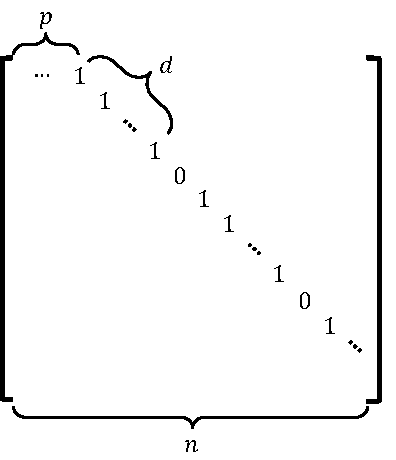
\includegraphics[width=3.0in]{fig/nilpotent_matrix.pdf}
	\caption{Nilpotent Matrix. $p$ off-diagonal offset, $d$ number of continuous $1$, and $n$ matrix dimension.}
	\label{fig:nilpotent}
\end{figure}

\subsection{Numerical Algorithm}

As shown in Algorithm \ref{alg:matgen}, the procedure of SMG2S is simple. Firstly, it reads an array $Spec_{in} \in \mathbb{C}^{n}$, as the given eigenvalues. Then it inserts random elements in $h$ lower diagonals of the initial matrix $M_0$, and sets its diagonal to be $Spec_{in}$, and scale it with $(2d)!$. Meanwhile, it generates a nilpotent matrix $A$ with the parameters $d$ and $p$. The final matrix $M_t$ can be generated as $M_t=\frac{1}{(2d)!}M_{2d}$, where $M_{2d}$ is the result after $2d$ times of loop $M_{i+1}=M_i+(\prod_{k=i+1}^{2d}k)(\widetilde{A_A})^i(M_0)$. The slight modification of the loop formula is to reduce the potential rounding errors coming from numerous division operations on modern computer systems.

\begin{algorithm*}[htbp]{}
	\caption{Matrix Generation Method}   
	\label{alg:matgen}   
	\begin{algorithmic}[1]
		\Function {matGen}{$input$:$Spec_{in} \in \mathbb{C}^n$, $h$, $d$, $output$: $M_t \in \mathbb{C}^{n\times n}$}
		\State Insert the entries in $h$ lower diagonals of $M_o \in \mathbb{N}^{n \times n}$
		\State Insert $Spec_{in}$ on the diagonal of $M_0$
		\State $M_0=(2d)!M_0$
		\State Generate nilpotent matrix $A \in \mathbb{C}^{n\times n}$ with selected parameters $d$ and $p$
		\For {\texttt{$i=0, \cdots, 2d-1$}}
		\State $M_{i+1}=M_i+(\prod_{k=i+1}^{2d}k)(\widetilde{A_A})^i(M_0)$
		\EndFor 
		\State $M_t = \frac{1}{(2d)!}M_{2d}$
		\EndFunction
	\end{algorithmic}
\end{algorithm*}

For $M_t$, if $M_0$ is a lower triangular matrix having $h$ non zero diagonals, it will be a band diagonal matrix, whose number of new diagonals in the upper triangular zone will be at most $2pd-1$. Thus the maximal number of the bandwidth of matrix $M_t$ is: $width = h + 2pd-1$, as in Fig. \ref{fig:matgen}. In general, researchers use these matrices to test the iterative methods of sparse linear systems. Thus after the generation of band matrix, it can be transferred to be sparse with the help of permutation matrices. Fig. \ref{fig:matgene} gives an example showing the pattern of the generated matrix by SMG2S. In general, researchers use these matrices to test the iterative methods for sparse linear systems. The $h$ lower diagonals of the initial matrix can set to be sparse, which ensures the sparsity of the final generated matrix, as shown in Fig. \ref{fig:matgene}. Moreover, the permutation matrix can also be applied to change the sparsity of the generated matrix further.

\begin{figure}[t]
	\centering
	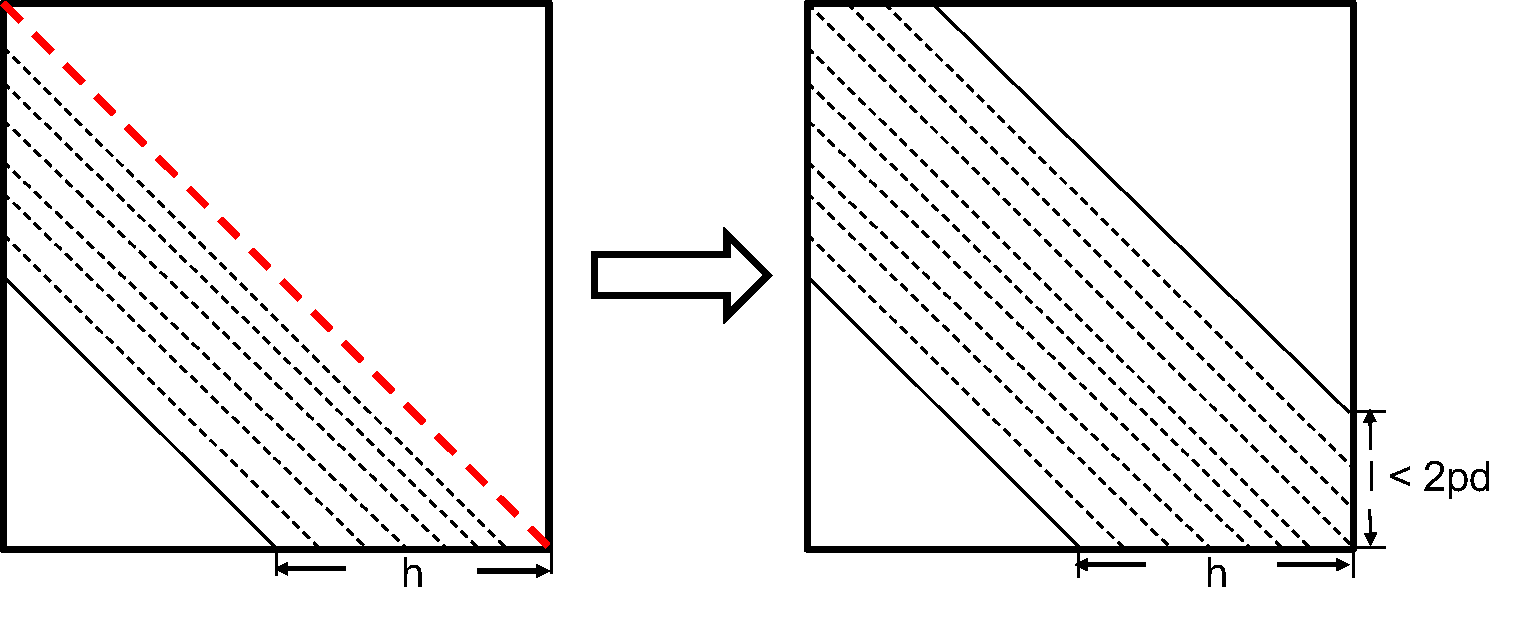
\includegraphics[width=5.8in]{fig/matgen.pdf}
	\caption{Matrix Generation. The left is the initial matrix $M_0$ with given spectrum on the diagonal, and the $h$ lower diagonals with random values; the right is the generated matrix $M_t$ with nilpotency matrix determined by the parameters $d$ and $p$.}
	\label{fig:matgen}
\end{figure}

The operations complexity $C$ of Algorithm \ref{alg:matgen} is given as: 

\begin{equation}
\label{eq:serial time}
\begin{aligned}
%C=(2d^2+(5+2h)d+(3h-4))n+\frac{h(h+1)(2d+1)}{2}-2(d+2).
C\approx 2(2d^2+(4h-2)d-(h+5))n-h(h+1)(h+4d-4).
\end{aligned}
\end{equation}

In Equation (\ref{eq:serial time}), the complexity of SMG2S is $max(\mathcal{O}(hdn),\mathcal{O}(d^2n))$. The worst case would be an $\mathcal{O}(n^3)$ problem for operations with large $d$ and $h$, and it would require $\mathcal{O}(n^2)$ memory storage. But if we want to generate a band matrix with small bandwidth which means $d \ll n$ and $h \ll n$, it turns to be a $\mathcal{O}(n)$ problem with good potential scalability and to consume $\mathcal{O}(n)$ memory storage.


\begin{figure}[t]
	\centering
	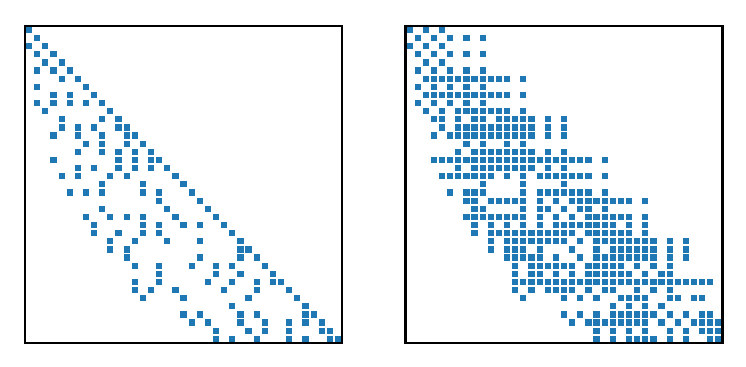
\includegraphics[width=5.2in]{fig/matgen/matgen.eps}
	\caption{Matrix Generation Pattern Example.}
	\label{fig:matgene}
\end{figure}

\section{Parallel Impementation and Evaluation}

In this section, we present the parallel implementation of SMG2S for homogeneous and heterogeneous clusters. The former is initially implemented based on MPI and PETSc, and the latter is based on MPI, CUDA, and PETSc. We select the mature library PETSc firstly since it provides several methods to verify the generated matrices, and also the basic operations inside are optimized for different computer architectures. After the validation of matrix generation based on PETSc, an open source parallel software with specific optimized communication is also implemented based on MPI and C++.

\subsection{Basic Implementation on CPUs}

For the initial CPU implementation, we chose PETSc instead of ScaLAPACK because we would like to evaluate the solvers for sparse linear systems. As shown in Algorithm \ref{alg:matgen}, the kernel of generation is the sparse matrix-matrix multiplication (SpGEMM) of $AM$ and $MA$, and the matrix-matrix addition (AYPX operation) as $AM-MA$. All the sparse matrices during the generation procedure are stored by the block diagonal Compressed Sparse Row (CSR) format which is provided in default by PETSc. We use the matrix operations supported by PETSc to facilitate the implementation. The block diagonal parallel matrix based on MPI are partitioned and stored into several submatrices. For example, if there are three MPI process: $proc1$, $proc2$ and $proc3$, the matrix can be divided into blocks as the Formula (\ref{parallelmat}). The submatrix $A$, $B$ and $C$ is stored in $proc1$,  $D$, $E$ and $F$ in $proc2$, and $G$, $H$ and $I$ is stored in $proc3$. On each process, the diagonal part and the off-diagonal are separately stored into two sequence block matrices. The parallel SpGEMM and AXPY operations for CPUs are already supported by PETSc \cite{balay2016petsc}. We use these functions directly to facilitate the implementation.


\begin{equation}
\label{parallelmat}
\left[
\begin{BMAT}(c)[4pt]{c|c|c}{c|c|c}
A  & B & C  \\
D & E & F  \\
G & H & I 
\end{BMAT}
\right]
\end{equation}


\subsection{Implementation on Multi-GPU}

\begin{figure}[t]
	\centering
	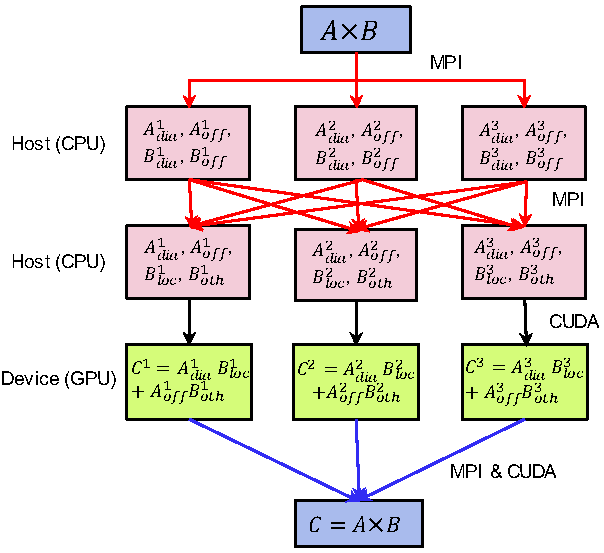
\includegraphics[width=5.in]{fig/spgemm2.pdf}
	\caption{The structure of a CPU-GPU implementation of SpGEMM, where each GPU is attached to a CPU. The GPU is in charge of the computation, while the CPU handles the MPI communication among processes.}
	\label{fig:cuda}
\end{figure}

PETSc does not supply the SpGEMM and AXPY operations for GPU clusters. Thus we implemented them using MPI, CUDA and cuSPARSE library based on the PETSc data structure definitions. The structure of implementation is given in Fig. \ref{fig:cuda} which uses sparse matrix $A$ and $B$ multiplication as an example. Firstly, the same as in PETSc, $A$ and $B$ are divided into slices, and each slice is saved in a process. In each process of number $i$, the local matrices are all saved as two separate sequence matrix, noted as $A^i_{dia}$ and $A^i_{off}$ for matrix $A^i$, $B^i_{dia}$ and $B^i_{off}$ for matrix $B^i$. Then $B^i_{dia}$ and $B^i_{off}$ are combined together as a novel sequence matrix noted as $B^i_{loc}$ in each process $i$. With MPI functionalities, each CPU gather all the remote data of matrix $B$ from the other processes, and construct them to a new sequence matrix $B^i_{oth}$. These matrices from each process are copied to one attached GPU, and calculate $C^i=A^i_{dia}B^i_{loc}+A^i_{off}B^i_{oth}$. The matrix operations on each GPU device is supported by the cuSPARSE. The final result $C$ can be obtained by gathering all slices $C_i$ from all the devices.

\subsection{Communication Optimized Implementation with MPI}

The implementation of SMG2S, especially the parallel SpGEMM kernel's communication can be specifically optimized based on the particular property of nilpotent matrix $A$. In fact, $A$ can be determined by three parameters $p$, $d$ and $n$ that we have mentioned in Section \ref{Matrix_Generation_Method}, thus it is not necessary to explicitly implement this parallel matrix. We note this nilpotent matrix as $A(p,d,n)$. Denote that for any matrix $J$, $J(i,j)$ represents the entry in row $i$ and column $j$; $J(i,:)$ represents all the entries of row $i$; and $J(:,j)$ represents all the entries of column $j$. Then, we observe the effects of right and left-multiplying this nilopotent matrix $A(p,d,n)$ on a general matrix $M$ by basic mathematical matrix operations. As shown in Fig. \ref{fig:am}, the right-multiplcation operation of $A(p,d,n)$ will shift all the entries of first $n-p$ columns to right side with an offset $p$. Denote $MA$ the result matrix gotten by the right-multiplying $A$ on $M$ (the result of $MA$ operation). We have $MA(:,j)=M(:,j-p), \forall j \in p,\cdots, n-1$, and $MA(:,j)=0,  \forall j \in 0,\cdots, p-1$. Similarly, the left-multiplying $A(p,d,n)$ on $M$ will shift the whole entries of last $n-p$ rows to up side with an offset $p$. Denote $AM$ the matrix gotten by the left-multiplying $A$ on $M$ (the result of $AM$ operation). We have $AM(i,:)=M(i+p,:), \forall i \in 0,\cdots, n-p-1$, and $AM(i:,)=0,  \forall i \in p,\cdots, n-1$. Moveover, the parameter $d$ decides that $MA(:,r(d+1))=0$ and $AM(r(d+1),:)=0$ with $r \in 1, \cdots, \lfloor \frac{n}{d+1}\rfloor$. 

\begin{figure*}[htbp]
	\centering
	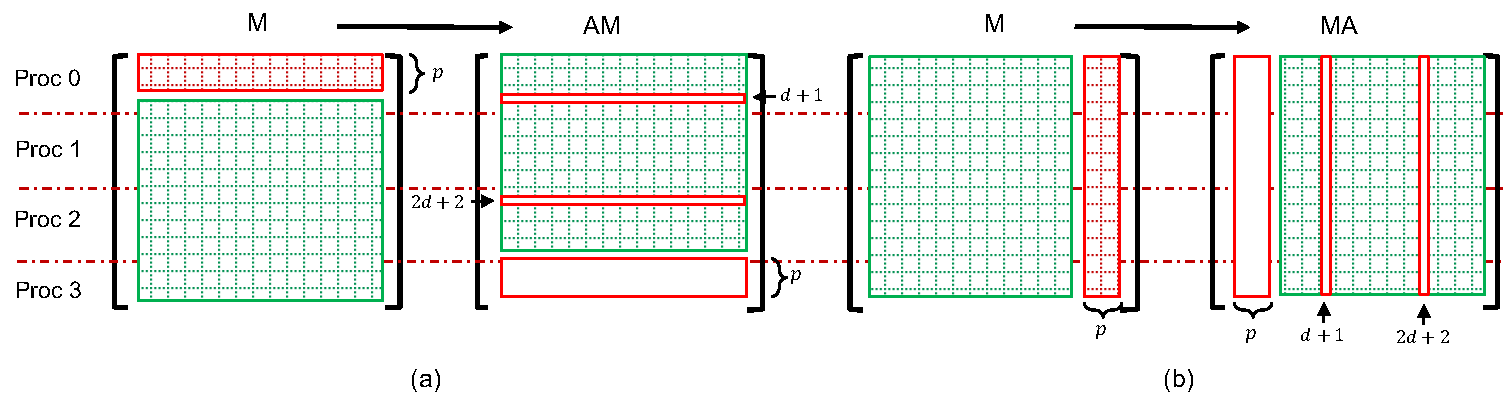
\includegraphics[width=6.2in]{fig/AMMA_2.pdf}
	\caption{(a) AM operation; (b) MA operation.}
	\label{fig:am}
\end{figure*}

When thinking about the implementation in parallel on distributed memory systems, the three integer parameters $p$, $d$ and $n$ can be shared by all MPI processes, and the parallel operations $AM$ and $MA$ are different from the general parallel SpGEMM, which is communication bounded. We analyze these two operations in Fig. \ref{fig:am}. Firstly, the general matrix $M$  is one-dimensional distributed by row across $m$ MPI process. As shown in  Fig. \ref{fig:am} (b), for $MA$, there is no communication inter different MPI processes since the data are moved inside each row. Assume that $ \lfloor \frac{n}{m}\rfloor \geq p$, for $AM$, the inter communication of MPI takes place when the MPI process $k$ ($k \in 1, \cdots, m-1$) should send the first $p$ rows of their sub-matrix to the closest previous MPI process numbering $k-1$. The communication complexity for each process is $\mathcal{O}(np)$. When generating the band matrix with low bandwidth $b$, it tends to be a $\mathcal{O}(bp)$ with $p=1$ or $2$. The MPI-based optimization implementations of AM and MA are respectively given by Algorithm \ref{alg:am} and \ref{alg:ma}. The communication inter MPI process is assumed by the asynchronous sending and receiving functions. In this algorithm, $M_k$, $MA_k$ and $AM_k$ imply the sub-matrices on process $k$ with $t$ rows. The rows and columns of these sub-matrices in Algorithm \ref{alg:am} and \ref{alg:ma} are all indexed by the local indices.

\begin{algorithm}[htbp]{}
	\caption{Parallel MPI AM Implementation}   
	\label{alg:am}   
	\begin{algorithmic}[1]
		\Function {AM}{$input$: matrix $M$, matrix row number $n$, $p$, $d$, proc number $m$; $output$: matrix $AM$}
		\State Distribute $t$ row blocks $M_k$ of $M$ to MPI process $k$
		\For {$p+1 \leq i < t $}
		\For {$0 \leq j < n$}
		\If{$M(i,j) \neq 0$}
		\State $AM_k(i-p,j) = M_k(i,j)$
		\EndIf
		\EndFor
		\EndFor
		\For {$0 \leq i < p $}
		\If {$k \neq 0$}
		\State $isend$ $ith$ $row$ $M_k(i)$ to $k-1$
		\EndIf
		\If {$k \neq m-1$}
		\State $irecv$ $ith$ $row$ $M_k(i)$ from $k+1$
		\State $AM_k(t-p+i)=M_k(i)$
		\EndIf
		\EndFor
		\EndFunction
		
	\end{algorithmic}  
	
\end{algorithm}

The communication-optimized SMG2S is implemented based on MPI and C++. The submatrix on each process is stored in ELLPACK format, using the key-value map containers provided by C++. The key-value map implementation facilitates the indexing and moving of the rows and columns. We did not implement a GPU version of SMG2S with this kind of communication since its core is the data movement among different computing units, which is not well suitable for multi-GPU architecture.


\begin{algorithm}[htbp]{}
	\caption{Parallel MPI MA Implementation} 
	\label{alg:ma}   
	\begin{algorithmic}[1]
		\Function {MA}{$input$: matrix $M$, matrix row number $n$, $p$, $d$, proc number $m$; $output$: matrix $MA$}
		\State Distribute $t$ row blocks $M_k$ of $M$ to process $k$ 
		\For {$0 \leq i < t $}
		\For {$p+1 \leq j < n$}
		\If{$M_k(i,j) \neq 0$}
		\State $MA_k(i,j+p) = M_k(i,j)$
		\EndIf
		\EndFor
		\EndFor 
		\EndFunction
	\end{algorithmic} 
	
\end{algorithm}

\section{Parallel Performance Evaluation}
\subsection{Hardware}
In experiments, we implement SMG2S on the supercomputers \textit{Tianhe-2} and \textit{Romeo}. \textit{Tianhe-2} system has been 6 times No.1 and is No.2 in the Top500 list, which is installed at the National Super Computer Center in Guangzhou of China. It is a heterogeneous system made of Intel Xeon CPUs and Intel Knights Corner (KNC), with 16000 compute nodes in total. Each node composes 2 Intel Ivy Bridge 12 cores @ 2.2 GHz. \textit{Romeo} is located at University of Reims Champagne-Ardenne, France. It is also a heterogeneous system made of Xeon CPUs and Nvidia GPUs, with 130 BullX R421 nodes. Each node composes 2 Intel Ivy Bridge 8 cores @ 2.6 GHz and 2 NVIDIA Tesla K20x GPUs. In this article, we do not test SMG2S using the KNC on \textit{Tianhe-2} since our parallel implementation does not support it with good performance.
\subsection{Strong and Weak Scalability Evaluation}

\begin{table}[htbp]
	\centering
	\caption{Details for weak scaling and speedup evaluation.}
	\renewcommand{\arraystretch}{1.5}
	\small
	\subfloat[Subtable 1 list of tables text][Matrix size for the CPU weak scaling tests on $Tianhe$-2.]{
		\begin{tabular}{|x{2.6cm}|x{1.4cm}|x{1.4cm}|x{1.4cm}|x{1.4cm}|x{1.4cm}|x{1.4cm}|}
			\hline
			CPU number & 48 & 96 & 192 & 384 & 768 & 1536\\
			\hline
			matrix size & $1\times10^6$ & $2\times10^6$  & $4\times10^6$  & $8\times10^6$  & $1.6\times10^7$  & $3.2\times10^7$ \\
			\hline
	\end{tabular}}
	\qquad
	\subfloat[Subtable 2 list of tables text][Matrix size for the CPU weak scaling on $ROMEO$.]{
		\begin{tabular}{|x{2.6cm}|x{1.5cm}|x{1.5cm}|x{1.5cm}|x{1.5cm}|x{1.5cm}|}
			\hline
			CPU number & 16 & 32 & 64 & 128 & 256\\
			\hline
			matrix size & $4\times10^5$ & $8\times10^5$ & $1.6\times10^6$ & $3.2\times10^6$ & $6.4\times10^6$\\
			\hline
	\end{tabular}}
	
	\subfloat[Subtable 3 list of tables text][Matrix size for the GPU weak scaling and speedup evaluation on $ROMEO$.]{
		\begin{tabular}{|x{3.8cm}|x{1.4cm}|x{1.4cm}|x{1.4cm}|x{1.4cm}|x{1.4cm}|}
			\hline
			CPU or GPU number & 16 & 32 & 64 & 128 & 256\\
			\hline
			matrix size &$2\times10^5$ & $4\times10^5$ & $8\times10^5$ & $1.6\times10^6$ & $3.2\times10^6$\\
			\hline
	\end{tabular}}
	\label{table:matrixsize}
\end{table}

In this section, we will use double-precision real and complex values to evaluate the strong and weak scalability of SMG2S's different implementations on CPU and multiple GPUs. All the test matrices in this paper are generated with the $h$ set to be $10$  and $d$ to be $7$. The details of the weak scaling experiments are given in Table \ref{table:matrixsize}. The matrix size of the strong scaling experiments on $Tianhe-2$ with CPUs, $ROMEO$ with CPUs and $ROMEO$ with GPUs are respectively $\num[round-precision=2,round-mode=figures]{16000000}$, $\num[round-precision=2,round-mode=figures]{3200000}$ and $\num[round-precision=2,round-mode=figures]{800000}$. The results are given in Fig. \ref{fig:scaling-cpu-tianhe-2}, Fig. \ref{fig:scaling-cpu-romeo} and Fig. \ref{fig:scaling-gpu-romeo}. The weak scaling for the PETSc implementation of SMG2S on \textit{Tianhe-2} trends to be bad when MPI processes number is larger than $768$, where the communication overhead becomes dominant for computation. But for the communication optimized SMG2S, both the strong and weak scaling perform well when the MPI process number is larger than $768$. The experiments show that SMG2S implemented with GPUs can still have good strong and weak scalability. In conclusion, SMG2S has always good strong scaling performance when $d$ and $h$ are much smaller than the dimension of the matrix $n$, because it turns to be a $\mathcal{O}(n)$ problem. The weak scalability is good enough for most cases. The reason is that the nilpotent matrix $A$ in SpGEMM is simple with not many non-zero elements, therefore there is not enormous communication among different computing units. The weak scalability has its drawback in case that the computing unit number come to be huge for the SMG2S implementation based on PETSc, where the communication overhead become dominant. The special implementation of communication-optimized SMG2S makes his strong and weak scalability better. It is also shown that the double precision complex type matrix generation takes almost two times time over the double precision real type for the basic SMG2S implementation, but the time consumption of complex and real type matrix generation of optimized SMG2S seems similar. The reason is that there is no numerical values multiplication anymore in the optimized implementation of SMG2S. 

\begin{figure}[htbp]
	\centering
	\subfloat[CPU strong scaling on Tianhe-2.]{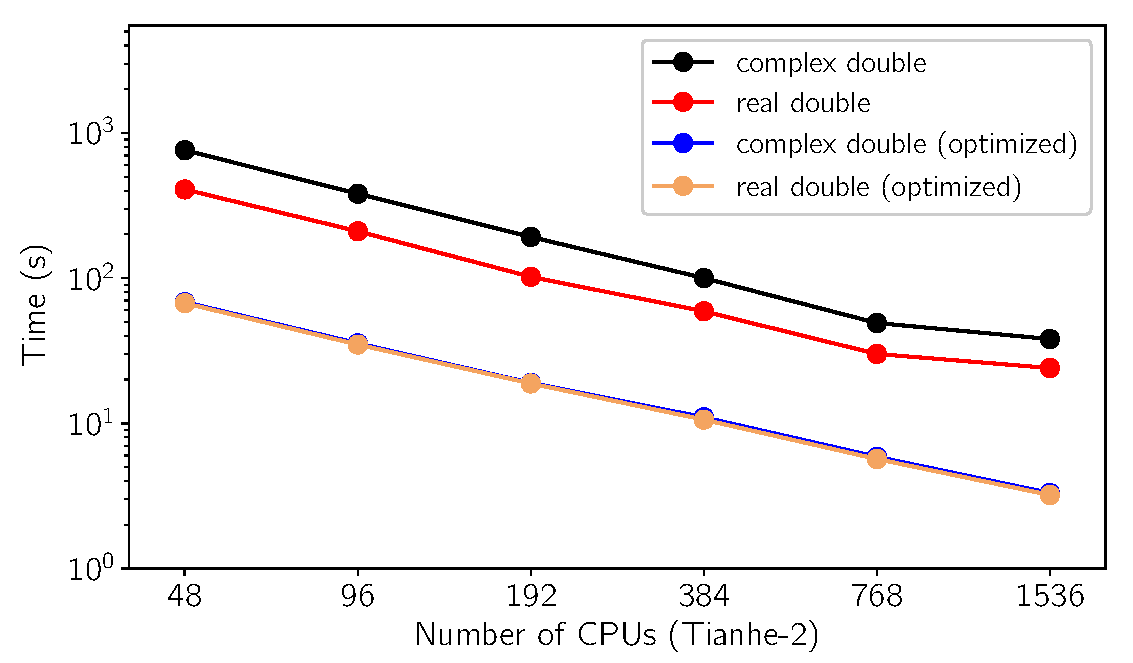
\includegraphics[width=3.1in]{fig/matgen/cpu_th2_strong_scalable.eps}%
		\label{ss_tianhe}}
	\subfloat[CPU weak scaling on Tianhe-2.]{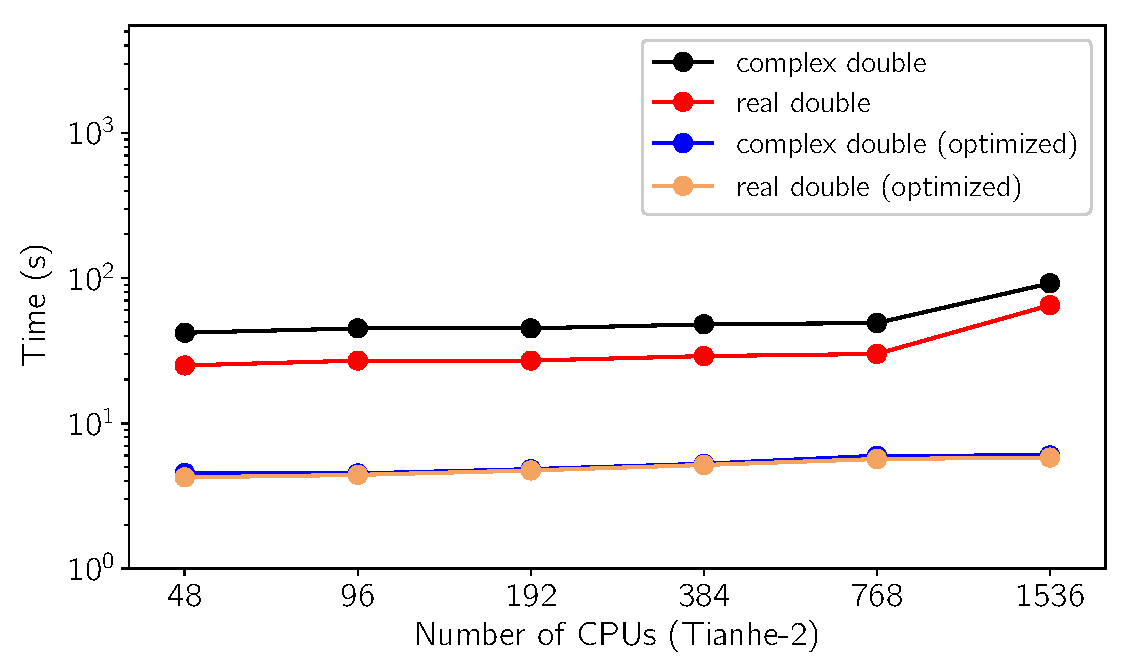
\includegraphics[width=3.1in]{fig/matgen/cpu_th2_weak_scalable.eps}%
		\label{ws_tianhe}}
	\caption{Strong and weak scaling results of SMG2S on different platforms. A base 2 logarithmic scale is used for X-axis, and a base 10 logarithmic scale for Y-axis. }
	\label{fig:scaling-cpu-tianhe-2}
\end{figure}

\begin{figure*}[htbp]
	\centering
	\subfloat[CPU strong scaling on ROMEO.]{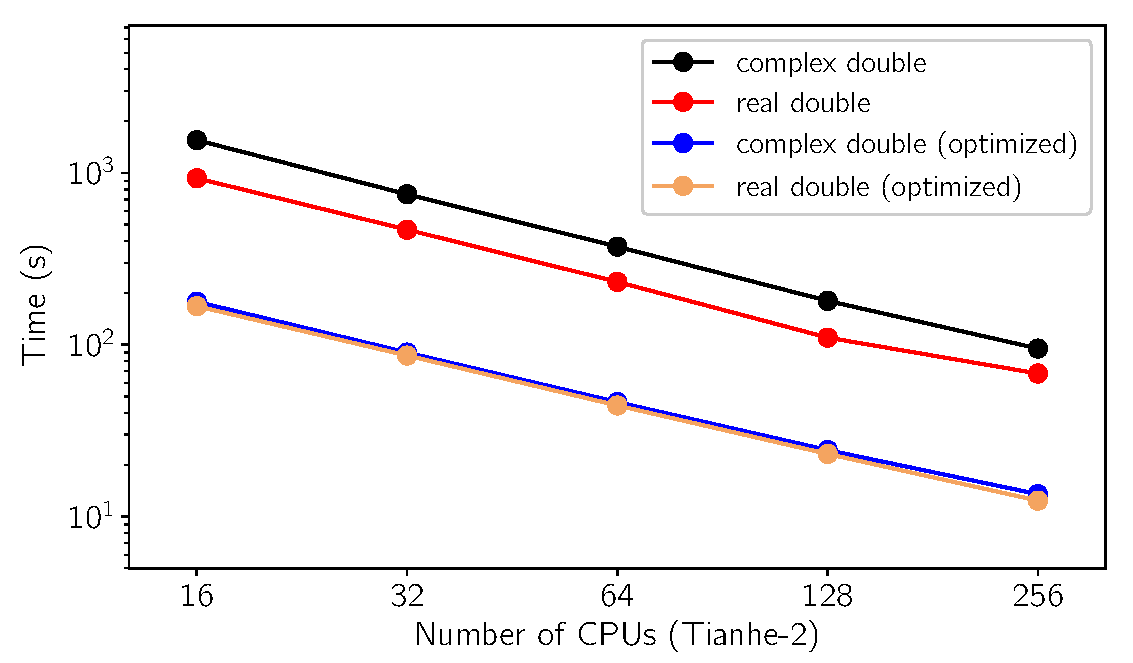
\includegraphics[width=3.1in]{fig/matgen/cpu_romeo_strong_scalable.eps}%
		\label{romeo}}
	\subfloat[CPU weak scaling on ROMEO.]{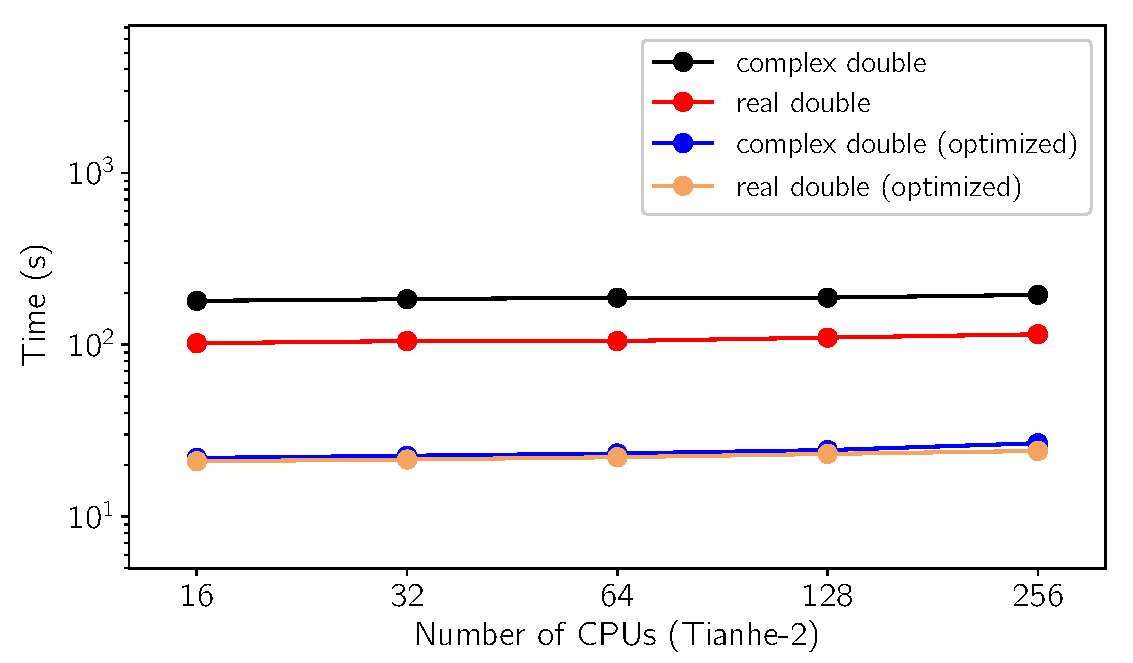
\includegraphics[width=3.1in]{fig/matgen/cpu_romeo_weak_scalable.eps}%
		\label{romeo_gpu}}
	\caption{Strong and weak scaling results of SMG2S on different platforms. A base 2 logarithmic scale is used for X-axis, and a base 10 logarithmic scale for Y-axis. }
	\label{fig:scaling-cpu-romeo}
\end{figure*}

\begin{figure*}[htbp]
	\centering
	\subfloat[GPU strong scaling on ROMEO.]{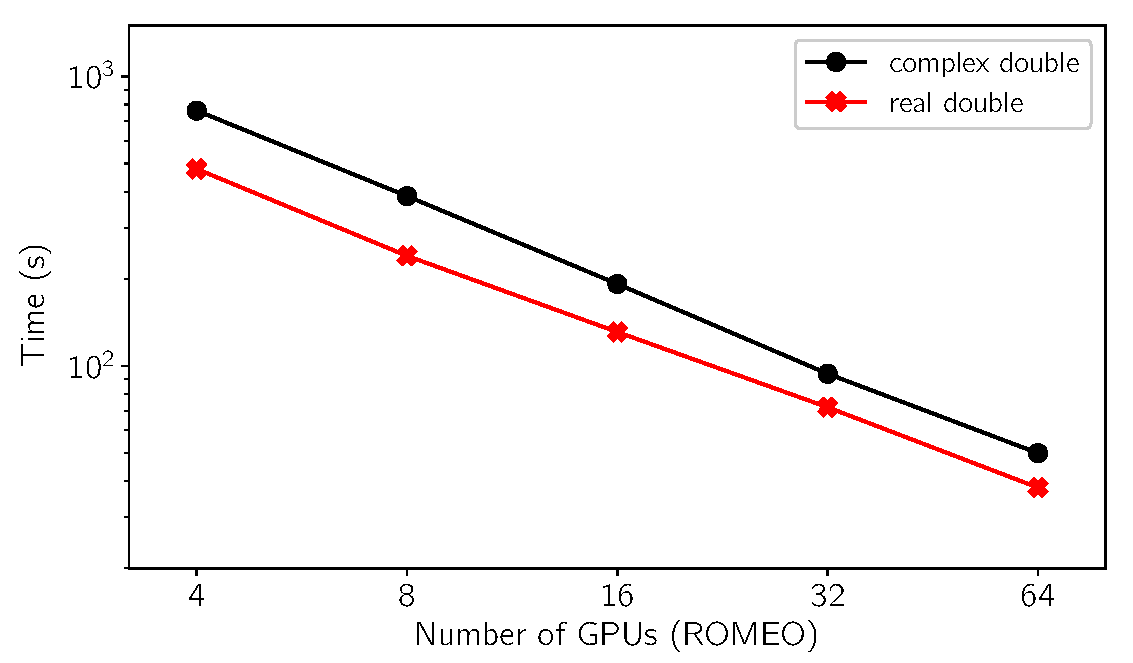
\includegraphics[width=3.1in]{fig/matgen/gpu_strong_scalable.eps}%
		\label{ss_romeo_gpu}}
	\subfloat[GPU weak scaling on ROMEO.]{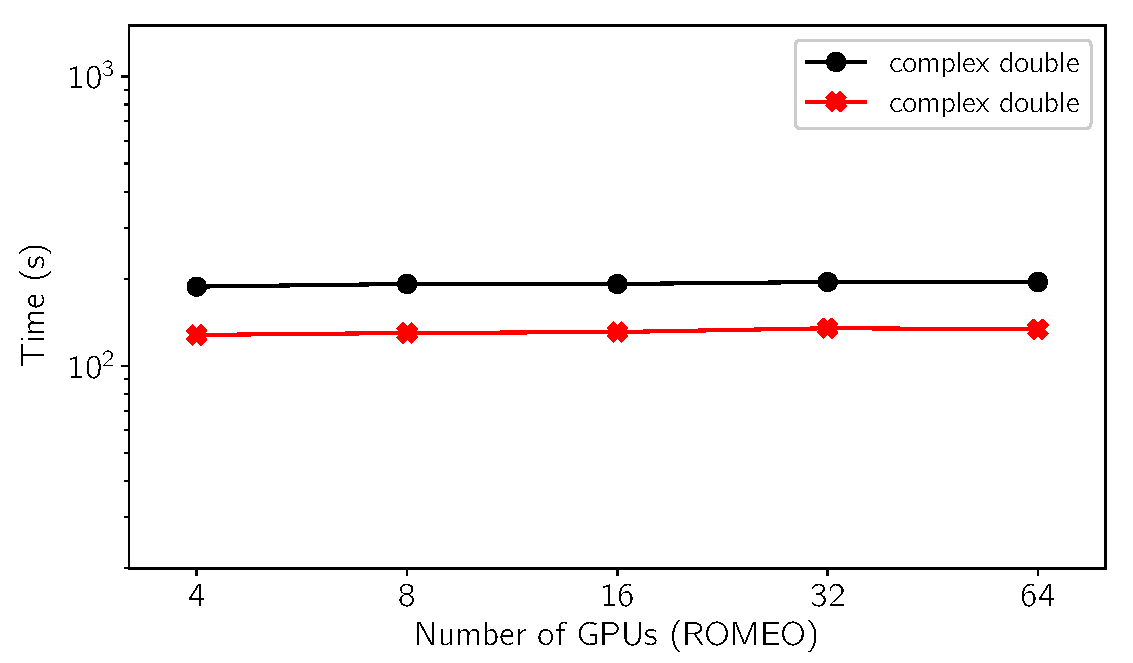
\includegraphics[width=3.1in]{fig/matgen/gpu_weak_scalable.eps}%
		\label{ws_romeo_gpu}}
	\caption{Strong and weak scaling results of SMG2S on different platforms. A base 2 logarithmic scale is used for X-axis, and a base 10 logarithmic scale for Y-axis. }
	\label{fig:scaling-gpu-romeo}
\end{figure*}

\begin{figure*}
	\centering
	\hfil
	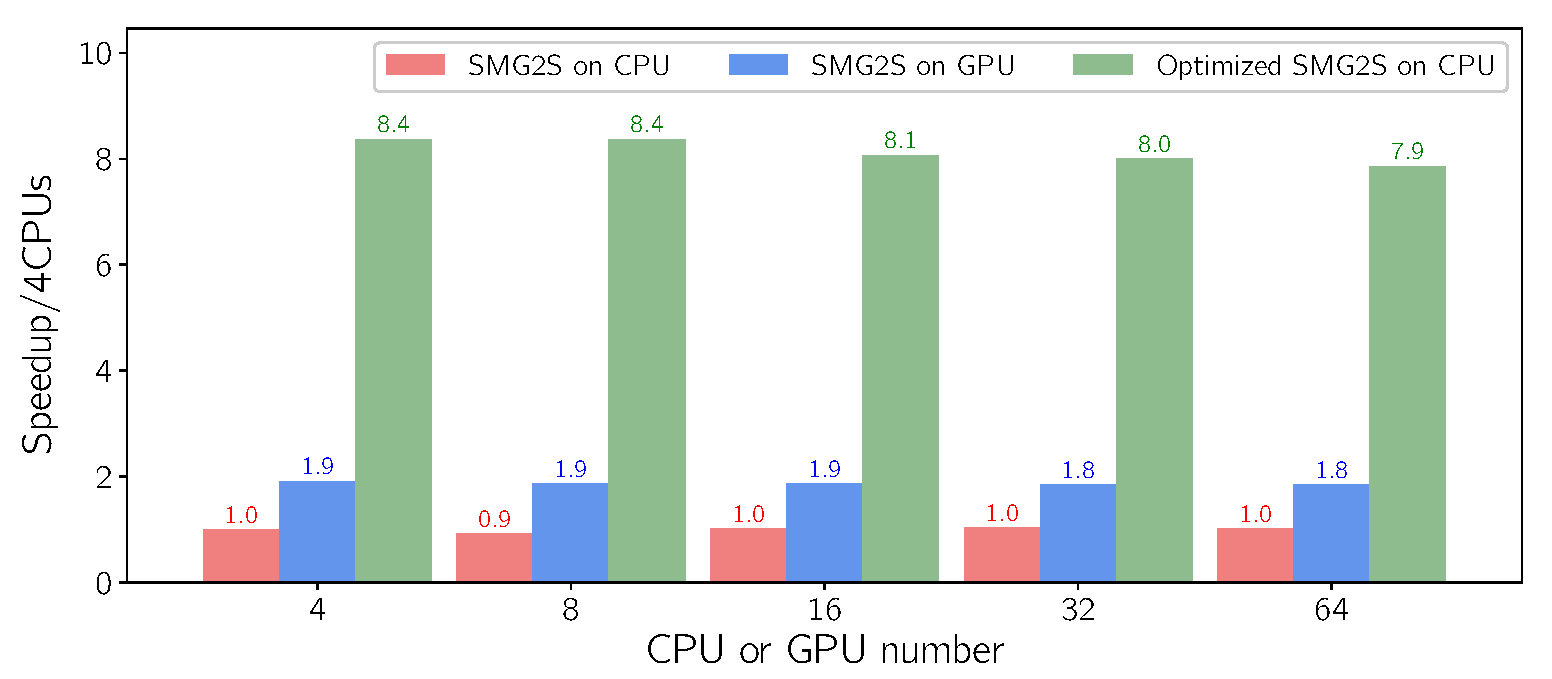
\includegraphics[width=6.2in]{fig/matgen/speedup.eps}%
	\caption{Weak scaling speedup comparison of GPUs on ROMEO.}
	\label{speedup}
\end{figure*}

\subsection{Speedup Evaluation}

The speedup of both SMG2S on multi-GPU and communication-optimized SMG2S on the CPUs compared with the PETSc-based implementation on CPU are also tested on \textit{Romeo}. According to the previous evaluation that complex and real value types always have good scalability, we select the double precision complex values for the speedup evaluation. The details of experiments are also given in Table \ref{table:matrixsize}c. The results are shown in Fig. \ref{speedup}. We can find that the GPU version of SMG2S has almost $1.9\times$ speedup over the PETSc CPU version. The communication-optimized SMG2S on CPUs has about $8\times$ speedup over the basic PETSc CPU version.

\subsection{Performance Analysis}

In conclusion, SMG2S always has good strong scalability when $d$ and $h$ are much smaller than the dimension of the matrix to be generated $n$, because It turns to be a $\mathcal{O}(n)$ problem. The weak scalability is good enough for most cases. The reason is that the matrices dealt with in SpGEMM are simple with not many non-zero elements. Therefore there are not enormous communication among different computing units. The weak scalability has its drawback in case that the computing unit number come to be huge for the SMG2S implementation based on PETSc, where the communication overhead become dominant. The strong and weak scaling for communication optimized SMG2S is good with its special implementation. It is also shown that the double-complex type matrix generation takes almost two times time over the double-real type for the basic SMG2S implementation. The time consumption of complex and real type matrix generation of optimized SMG2S seems similar. The reason is that in the optimized implementation of SMG2S, there are not numerical values multiplication anymore.  It also has the capacity to take advantage of GPUs to accelerate the computation with about $1.9$x speedup than CPUs. The communication optimized version has $8$x speedup over the basic implementation.

\section{Verification Method}

In the last section, we show the good parallel performance of SMG2S, and then it is necessary to verify if the generated matrices are able to keep the given spectra with enough accuracy. Generally, the iterative eigenvalue solvers such as the Arnoldi or other Krylov methods (\cite{petiton1992parallel}) are applied to approximate the dominant eigenvalues. However, the accuracy verification is an opposite case. Now there exists a value, and we want to check if it is an eigenvalue of a given matrix. These iterative methods cannot directly and efficiently deal with this kind of verification. In this section, we present a method for accuracy verification using the Shifted Inverse Power method, which was easily implemented in parallel.

The Power method is an algorithm to approximate the greatest eigenvalue. Meanwhile, the Inverse Power method is a similar iterative algorithm to find the smallest eigenvalue. The middle eigenvalues can be obtained by the Shifted Inverse Power method (\cite{hernandez2005single}).  This method is given in Algorithm \ref{alg:inversePower}. Its operation complexity is $\mathcal{O}(n^3)$. The Shifted Inverse Power method is used to compute the eigenvalue which is the nearest one to a given value in a few steps of iterations. The related eigenvector can be easily calculated by its definition and used to check if this given value is an eigenvalue of the matrix.

\begin{algorithm}[htbp]{}
	\caption{ Shifted Inverse Power method}   
	\label{alg:inversePower}   
	\begin{algorithmic}[1]
		\Function {sipm}{$input$: Matrix $A$, initial guess for desired eigenvalue $\sigma$, initial vector $v_0$, $output$: Approximate eigenpair ($\theta$, $v$)}
		\State $y=v_0$
		\For {\texttt{$i=1,2,3 \cdots$}}
		\State $\theta=||y||_\infty$
		\State $v=y/\theta$
		\State Solve $(A-\sigma I)y=v$
		\EndFor 
		\EndFunction
	\end{algorithmic}  
\end{algorithm}

\begin{figure}[htbp]
	\centering
	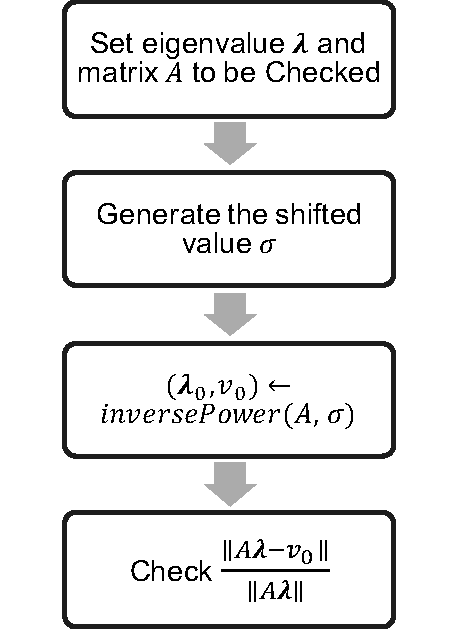
\includegraphics[width=6.2in]{fig/smg2s-check.pdf}
	\caption{SMG2S verification workflow.}
	\label{smg2s-check}
\end{figure}

In details, for checking if the given value $\lambda$ is the eigenvalue of a matrix, we select a shifted value $\sigma$ which is close enough to $\lambda$. An eigenpair $(\lambda', v')$ with the relation $Av'=\lambda' v'$ can be approximated in very few steps by Shifted Inverse Power method, with $\lambda'$ is the closest eigenvalue to $\sigma$. Since $\sigma$ is very close to $\lambda$, it should be that $\lambda$ and $\lambda'$ are the same eigenvalue of a system, and $v'$ should be the eigenvector related to $\lambda$. In reality, even if the computed eigenvalue is very close to the true one, the related eigenvector may be quite inaccurate. For the right eigenpairs, the formula $Av'\approx\lambda v'$ should be satisfied. Based on this relation, we define the relative error as Formula (\ref{check}) to quantify the accuracy. 

\begin{equation}
\label{check}
error=
\frac{||Av'-\lambda v'||}{||Av'||}
\end{equation}

If $\lambda' = \lambda$, this $error$ should be $0$, if not, this generated matrix do not have an exact eigenvalue as $\lambda$. In real experiments, the exact solution cannot always be guaranteed with the arithmetic rounding errors of floating operations during the generation. A threshold could be set for accepting it or not.

\begin{table}[htbp]
	\renewcommand{\arraystretch}{1.4}
	\small	
	\caption{Accuracy Verification Results.}
	\label{accuracy}
	\centering
	\begin{tabular}{ccccc}
		\toprule
		Matrix $N^{o}$& Size & Spectra & Acceptance (\%) & max $error$ \\
		\midrule
		1  & 100 & $Spec1$ &93&\num[round-precision=2,round-mode=figures]{0.02}\\
		2 & 100 & $Spec2$   & 94&\num[round-precision=2,round-mode=figures]{0.03}\\
		3 & 100 & $Spec3$  &100&\num[round-precision=2,round-mode=figures]{0.00007}\\
		4 & 100 & $Spec4$  &100&\num[round-precision=2,round-mode=figures]{0.0000003}\\
		\bottomrule
	\end{tabular}
\end{table}

\subsection{Experimental Results}

In the experiments, we test the accuracy of SMG2S with four selected cases among the various tests of different spectral distributions. Fig. \ref{fig_1_case} and Fig. \ref{fig_2_case} are cases of clustered eigenvalues with different scales. Fig. \ref{fig_second_case} is a special case with the dominant part of eigenvalues clustered in a small region. Fig. \ref{fig_forth_case} is a case that composes the conjugate and closest pair eigenvalues. These figures compare the difference between the given spectra (noted as initial eigenvalues in the figures) and the approximated ones (noted as computed eigenvalues) by the Shifted Inverse Power Method. Clearly, the matrices generated by SMG2S can keep almost all the given eigenvalues in the four cases even they are very clustered and close. The acceptance threshold is set to be $1.0\times 10^{-3}$.

This acceptance for cases of Fig. \ref{fig_1_case}, Fig. \ref{fig_2_case}, Fig. \ref{fig_second_case} and Fig. \ref{fig_forth_case} are respectively 93\%, 100\%, 94\% and 100\%. The maximum $error$ for them are respectively \num[round-precision=2,round-mode=figures]{0.03}, \num[round-precision=2,round-mode=figures]{0.00007}, \num[round-precision=2,round-mode=figures]{0.03} and \num[round-precision=2,round-mode=figures]{0.0000003}.  After the tests, we conclude that SMG2S is able to keep accurately the given spectra even for the very clustered and closest eigenvalues. In some cases, a very little number of too clustered eigenvalues may result in the inaccuracy of given ones, but in general, the generated matrix can fufil the need to evaluate the linear system and eigenvalue solvers. 

\begin{figure}[htbp]
	\centering
	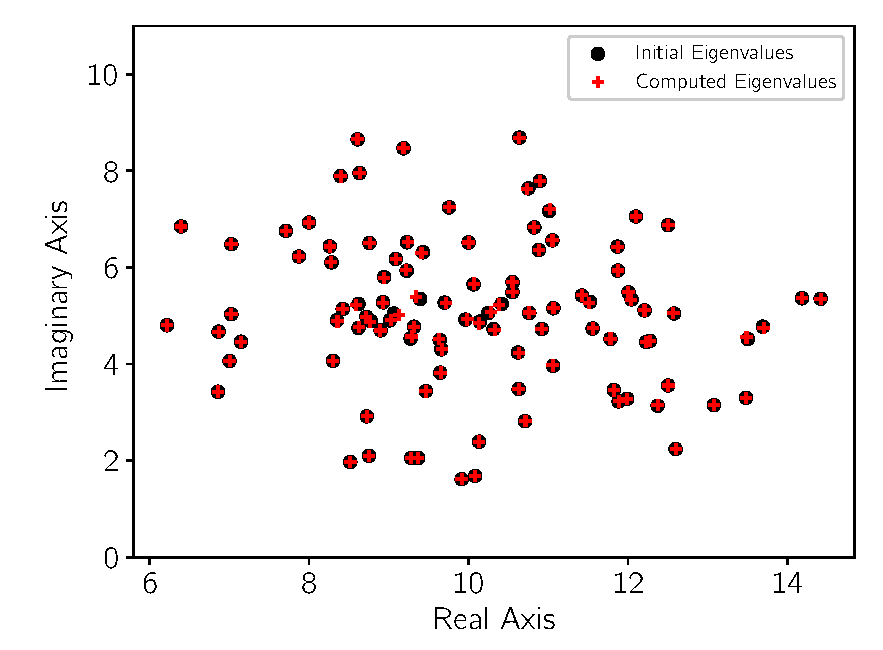
\includegraphics[width=5.8in]{fig/matgen/vector1.eps}
	\caption{Spec1: Clustered Eigenvalues I.}
	\label{fig_first_case}
\end{figure}

\begin{figure}[htbp]
	\centering
	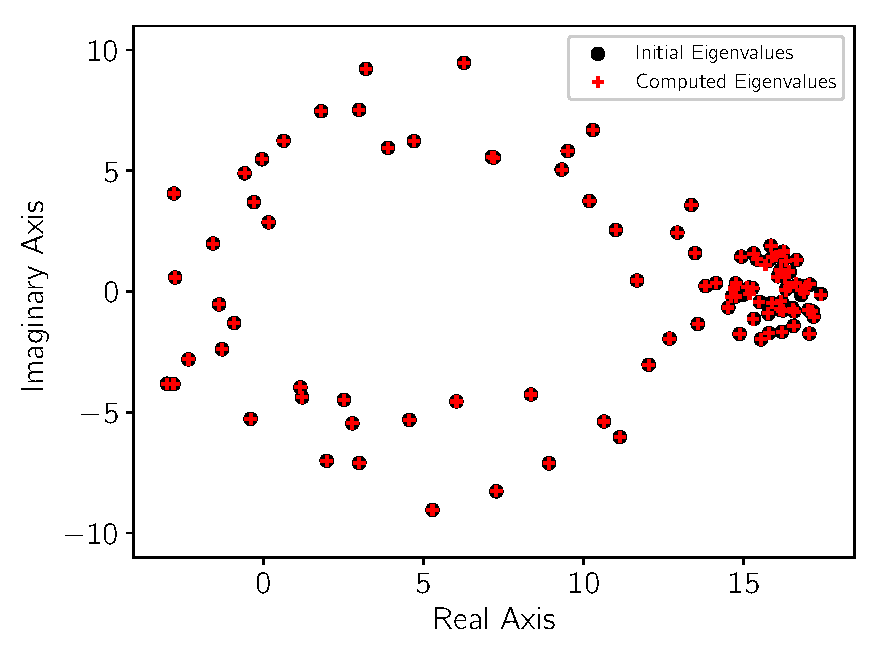
\includegraphics[width=5.8in]{fig/matgen/vector2.eps}
	\caption{Spec1: Clustered Eigenvalues I.}
	\label{fig_second_case}
\end{figure}

\begin{figure}[htbp]
	\centering
	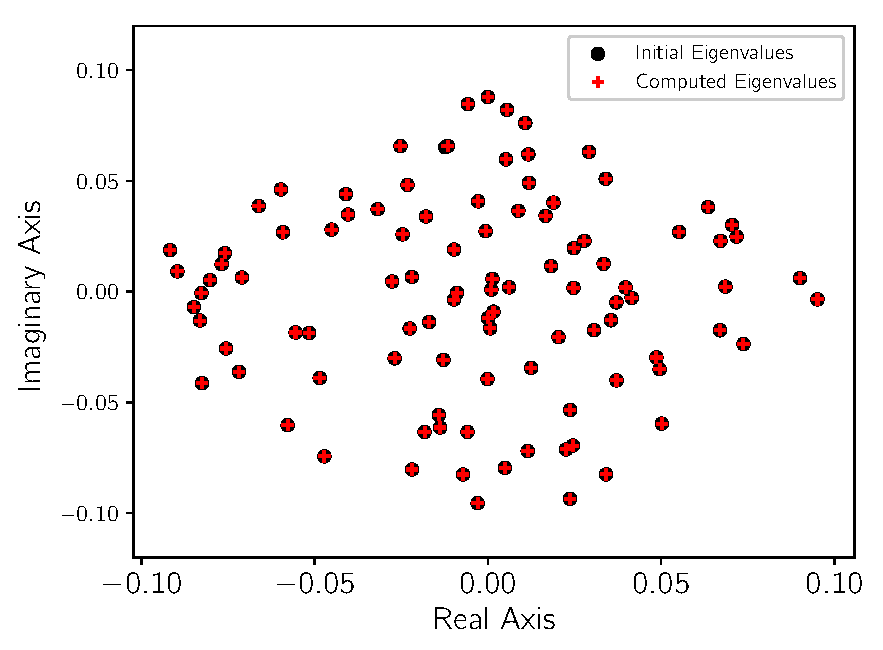
\includegraphics[width=5.8in]{fig/matgen/vector3.eps}
	\caption{Spec3: Clustered Eigenvalues III.}
	\label{fig_third_case}
\end{figure}

\begin{figure}[htbp]
	\centering
	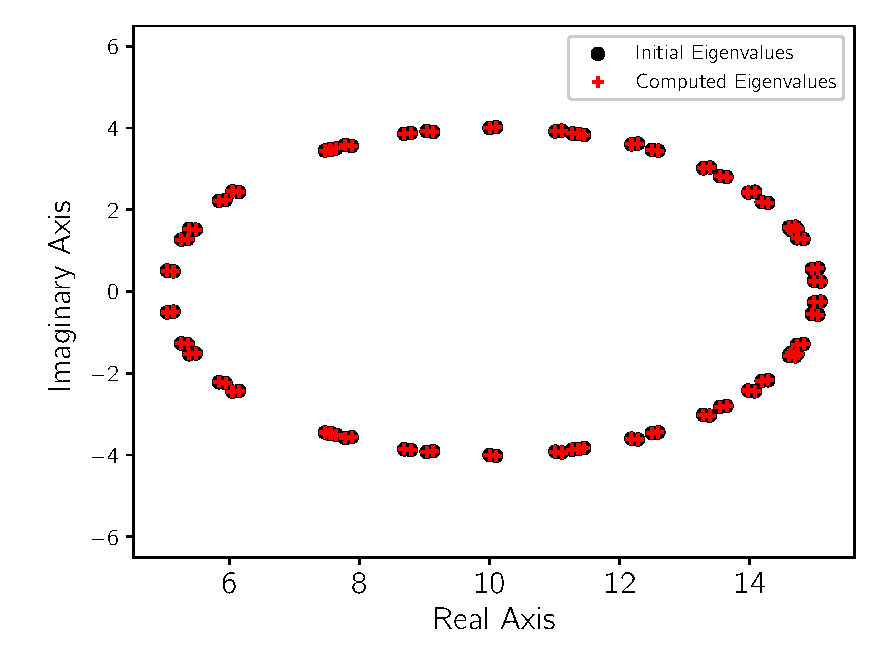
\includegraphics[width=5.8in]{fig/matgen/vector5.eps}
	\caption{Spec4: Conjugate and Closest Eigenvalues.}
	\label{fig_forth_case}
\end{figure}

\subsection{Arithmetic Precision Analysis}

Any floating operations will introduce rounding errors, which cannot be ignored for the generation of large matrices. Regarding the non-Hermitian matrix, its eigenvalues may be extremely sensitive to perturbation. This sensibility is bounded by $bound(\lambda) \leq ||E||_2Cond(\lambda)$, with $Cond(\lambda)$ the condition number of related eigenvalue $\lambda$ and $||E||_2$ the Euclidean norm of errors \cite{saad2011numerical}. $Cond(\lambda)=1$ for the Hermitian matrices, but for the non-Hermitian ones, it can be excessively high. There are two solutions facing this problem. The first one is to ensure the eigenvalue to be well-conditioned. The second is to use the integer value for the matrix generation, since only integers and the operations $+$, $-$, and $\times$ on the microprocessor can make absolutely exact computations. As shown in Algorithm \ref{alg:matgen}, most of the operations in SMG2S are $+$, $-$ and $\times$, except the step 8 with a division operation. Without step 8, we could introduce a special SMG2S fully using integers to avoid the risks of rounding errors. The spectra of the generated matrix will be $(2d)!$ times of the given one. Moreover, the upper band's width of generated depends on the parameter $d$. The factorial of $2d$ can easily reach the limit of integer, even with unsigned long long type. Thus a special factorial function using multiple integers should be implemented in order to enlarge the upper band's width.

\section{Package, Interface and Application}

SMG2S is packaged and released as an open source software based on MPI and C++. In this section, we present firstly the package information of SMG2S and its interface to various programming languages and scientific computational libraries. More details of package can be found in the related manual \cite{wu2018smg2s}.Then, we give an example which uses SMG2S to evaluate different Krylov solvers. 

\subsection{Package}

\subsubsection{Installation Prerequisites}

Before the use of SMG2S, the below packages and libraries should be available on the computer platforms:

\begin{enumerate}
	\item C++ Comiler with c++11 support;
	\item MPI;
	\item CMake (version minimum 3.6)
	\item (Optional) PETSc and SLEPc are necessary for the verification of accuracy of generated matrices to keep the given spectra.
\end{enumerate}

\subsubsection{Functions and Directory Structure}

SMG2S provides the following subsets of function, including the setup of parallel matrix and vector, the construction of special nilpotent matrix, the matrix generation function, the interfaces to other languages/libraries and the verification mechanism.

\begin{itemize}
	\item \textbf{Parallel Vector and Matrix:} this part presents the functions implemented in SMG2S to establish parallel vector and matrix over distributed memory platforms.
	\item \textbf{Nilpotent Matrix Object:} this part presents a special nilpotent matrix object for the matrix generation procedure in SMG2S.
	\item \textbf{Generating Matrix with prescribed eigenvalues:} this part gives the way to use SMG2S to generate required test matrices.
	\item \textbf{Interface to Other Languages/Libraries:} this part introduces the interface of SMG2S to other languages and existing scientific computational libraries such as PETSc and Trilinos.
	\item \textbf{Verification of Eigenvalues of Generated Matrix:} this part gives the way to verify the accuracy of eigenvalues of generated matrices comparing with given spectrum. A graphic user interface is also provided to facilitate the comparison.
\end{itemize}

\subsubsection{Generation Workflow}

SMG2S is a collection of C++ include headers, this section gives the workflow to generate test matrices by SMG2S. The C++ template support of SMG2S allows generating matrices of different sizes, scalar types, and precisions.


1. Include the head file

\begin{lstlisting}[language=C++,frame=single]
#include <smg2s/smg2s.h>
\end{lstlisting}

2. Generate the Nilpotent Matrix Object:

\begin{lstlisting}[language=C++,frame=single]
Nilpotency<int> nilp;
nilp.NilpType1(length,probSize);
\end{lstlisting}

3. Create the parallel Sparse Matrix Object Mt:

\begin{lstlisting}[language=C++,frame=single]
parMatrixSparse<std::complex<double>,int> *Mt;
\end{lstlisting}

4. Generate a new matrix by SMG2S:

\begin{lstlisting}[language=C++,frame=single]
MPI_Comm comm; //working MPI Communicator
Mt = smg2s<std::complex<double>,int>(probSize, nilp, 
lbandwidth, spectrum, comm);
\end{lstlisting}


Here, in step $4$, the \textbf{probsize} parameter represent the matrix size, \textbf{nilp} is the nilpotency matrix object that we have declared previously in step $2$, \textbf{lbandwidth} is the bandwidth of lower-diagonal band. \textbf{spectrum} is the file path of spectra file, if \textbf{spectrum} is set as \textbf{" "}, SMG2S will use the function provided inside to generate the spectral distribution. \textbf{comm} is the basic object used by MPI to determine which processes are involved in a communication.

The given spectra file is in \textbf{pseudo-Matrix Market Vector format}. For the complex eigenvalues, the given spectrum is stored in three columns as below, the first column is the coordinates, the second column is the real part of complex values, and the third column is the imaginary part of complex values.

\begin{lstlisting}[language=bash,frame=single]
%%MatrixMarket matrix coordinate complex general
3 3 3
1 10 6.5154
2 10.6288 3.4790
3 10.7621 5.0540
\end{lstlisting}

For the eigenvalues values, the given spectrum is stored in two columns as below, the first column is the coordinates, the second column is related values.

\begin{lstlisting}[language=bash,frame=single]
%%MatrixMarket matrix coordinate real general
3 3
1 10
2 10.6288
3 10.7621
\end{lstlisting}

If the users want to generate the eigenvalues in time without loading from local file, they can customize their eigenvalues generation by the function \textcolor{blue}{specGen} in the file \textcolor{blue}{./verification/tests/specGen.h}, and set the parameter \textcolor{blue}{spectrum} of \textcolor{blue}{smg2s} to be \textcolor{blue}{" "}.

\begin{lstlisting}[language=C++,frame=single]
template<typename T, typename S>
void parVector<T,S>::specGen(std::string spectrum)
\end{lstlisting}

In this function, the eigenvalues are stored by the distributed vector textcolor{blue}{parVector}. And the filling of values on this parVector can be done by  the method \textcolor{blue}{SetValueGlobal} implemented in \textcolor{blue}{parVector}, which takes the global indices to set values.

We know that the low band bandwidth of initial matrix can be set by the parameter  \textcolor{blue}{lbandwidth} of \textcolor{blue}{smg2s}. Additionaly, the distribution of entries of initial matrix can also be customized by the function  \textcolor{blue}{matInit} provided by the file \textcolor{blue}{./verification/tests/specGen.h}. En default, these entries are filled in random. The different mechanism to fill them will influence the sparsity of final generated sparse matrix.

\begin{lstlisting}[language=C++,frame=single]
template<typename T, typename S>
void matInit(
parMatrixSparse<T,S> *Am, 
parMatrixSparse<T,S> *matAop, 
S probSize, 
S lbandwidth
)
\end{lstlisting}

In this function, distributed matrix $Am$ and $matAop$ should be filled with the same way. And these entries of matrix can be filled by the method \textcolor{blue}{Loc\_SetValue} implemented in \textcolor{blue}{parMatrixSparse}. \textcolor{blue}{Loc\_SetValue} uses the \textcolor{red}{global indices} of matrix to set values.

\subsection{Interface To Scientific Libraries}

Until now, SMG2S provides interfaces to C, Python, PETSc and Trilinos.

\begin{figure}[htbp]
	\centering
	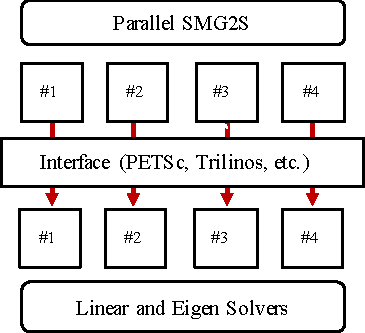
\includegraphics[width=3.6in]{fig/interface.pdf}
	\caption{SMG2S Workflow and Interface.}
	\label{fig:interface}
\end{figure}

\subsubsection{Interface to C}
SMG2S install command will generate a shared library \textcolor{blue}{libsmg2s.so} (\textcolor{blue}{libsmg2s2c.dylib} on OS X platform) into \$\{INSTALL\_DIRECTORY\}/lib. It can be used to profit the C wrapper of SMG2S. 

A minimum example to use the interface of SMG2S to C:

\begin{lstlisting}[language=C,frame=single]
#include <interface/C/c_wrapper.h>

/*create Nilpotency object*/
struct NilpotencyInt *n;
n = newNilpotencyInt();
NilpType1(n, 2, 10);
/*create the parallel Sparse Matrix Object*/
struct parMatrixSparseRealDoubleInt *m;
m = newParMatrixSparseRealDoubleInt();
/*Generation by SMG2S*/
smg2sRealDoubleInt(m, 10, n, 3 ," ",MPI_COMM_WORLD);
/*Release Nilpotency Object and parMatrixSparse Object*/
ReleaseNilpotencyInt(&n);
ReleaseParMatrixSparseRealDoubleInt(&m);
\end{lstlisting}

SMG2S provides the C interface to different data types. For the data type of matrix size, it can be either $int$ or $long int$; for the data type of matrix entries, it can be either $complex$ or $real$ with $single$ or $double$ precision.

C interface implements the Nilpotent Matrix object for both $int$ and $long$ $int$ as below:
\begin{lstlisting}[language=C,frame=single,	basicstyle=\footnotesize]
struct NilpotencyInt;
struct NilpotencyLongInt;
\end{lstlisting}

For all the public functions  in parMatrixSparse Object and smg2s function, \textbf{SUFFIX} below can be added them to provides the implementations for different data types:

\begin{multicols}{2}
	\begin{itemize}
		\item $ComplexDoubleLongInt$;
		\item $ComplexDoubleInt$;
		\item $ComplexSingleLongInt$;
		\item $ComplexSingleInt$;
		\item $RealDoubleLongInt$;
		\item $RealDoubleInt$;
		\item $RealSingleLongInt$;
		\item $RealSignleInt$.
	\end{itemize}
\end{multicols}

\subsubsection{Interface to Python}

SMG2S uses SWIG to generate the wrapper of SMG2S to Python. This interface is available through the Python pacjage management system \textit{pip}

\begin{lstlisting}[language=bash,frame=single]
#install online from pypi
CC=mpicxx pip install smg2s
#run
mpirun -np 2 python generate.py
\end{lstlisting}

Before the utilization, make sure that \textbf{mpi4py} is installed.

\subsubsection{Interface to PETSc}

SMG2S provides the interface to scientific computational softwares PETSc/SLEPc.

The way of Usage:

1. Include the header file:
\begin{lstlisting}[language=C,frame=single]
#include <interface/PETSc/petsc_interface.h>
\end{lstlisting}

2. Create parMatrixSparse type matrix :
\begin{lstlisting}[language=C,frame=single]
parMatrixSparse<std::complex<double>,int> *Mt;
\end{lstlisting}

3. Restore this matrix into CSR format :
\begin{lstlisting}[language=C,frame=single]
Mt->Loc_ConvertToCSR();
\end{lstlisting}

4. Create PETSc MAT type :
\begin{lstlisting}[language=C,frame=single]
MatCreate(PETSC_COMM_WORLD,&A); 
\end{lstlisting}

5. Convert to PETSc MAT format :

\begin{lstlisting}[language=C,frame=single]
A = ConvertToPETSCMat(Mt); 
\end{lstlisting}

Here are the example of \href{https://github.com/SMG2S/SMG2S/tree/master/example/arnoldi}{\textcolor{blue}{Arnoldi}}, \href{https://github.com/SMG2S/SMG2S/tree/master/example/gmres}{\textcolor{blue}{GMRES}}, and another  \href{https://github.com/SMG2S/SMG2S/tree/master/example/krylov}{\textcolor{blue}{Krylov method}}.

\subsubsection{Interface to Trilinos/Teptra}

SMG2S is able to convert its distributed to the CSR one-dimensional distributed matrix defined by Teptra in Trilinos.

The way of usage:

1. Include header file

\begin{lstlisting}[language=C++,frame=single]
#include <interface/Trilinos/trilinos_interface.hpp>
\end{lstlisting}

2. Create parMatrixSparse type matrix :
\begin{lstlisting}[language=C++,frame=single]
parMatrixSparse<std::complex<double>,int> *Mt;
\end{lstlisting}

3. Create Trilinos/Teptra MAT type :
\begin{lstlisting}[language=C++,frame=single]
parMatrixSparse<std::complex<double>,int> *Mt;
\end{lstlisting}

4. Convert to Trilinos MAT format :
\begin{lstlisting}[language=C++,frame=single]
K = ConvertToTrilinosMat(Mt); 
\end{lstlisting}

\href{https://github.com/SMG2S/SMG2S/tree/master/example/teptra}{Here is a full \textcolor{blue}{ example of Trilinos}.}

\subsection{Graphic User Interface for Verification}

When you launch the program, a new windows opens like Fig. \ref{fig:Home Screen Capture} :

After that, you can click on "Display" to build and open the graphic on the right side of the window. Click on "New window" to open your graphic on a new window. It's possible to open as many windows as you want like Fig. \ref{fig:Home Screen Plot Capture}:

\begin{figure}[htbp]
	\label{fig:Home Screen Plot Capture}
	\caption{Home Screen Plot Capture}
	\centering
	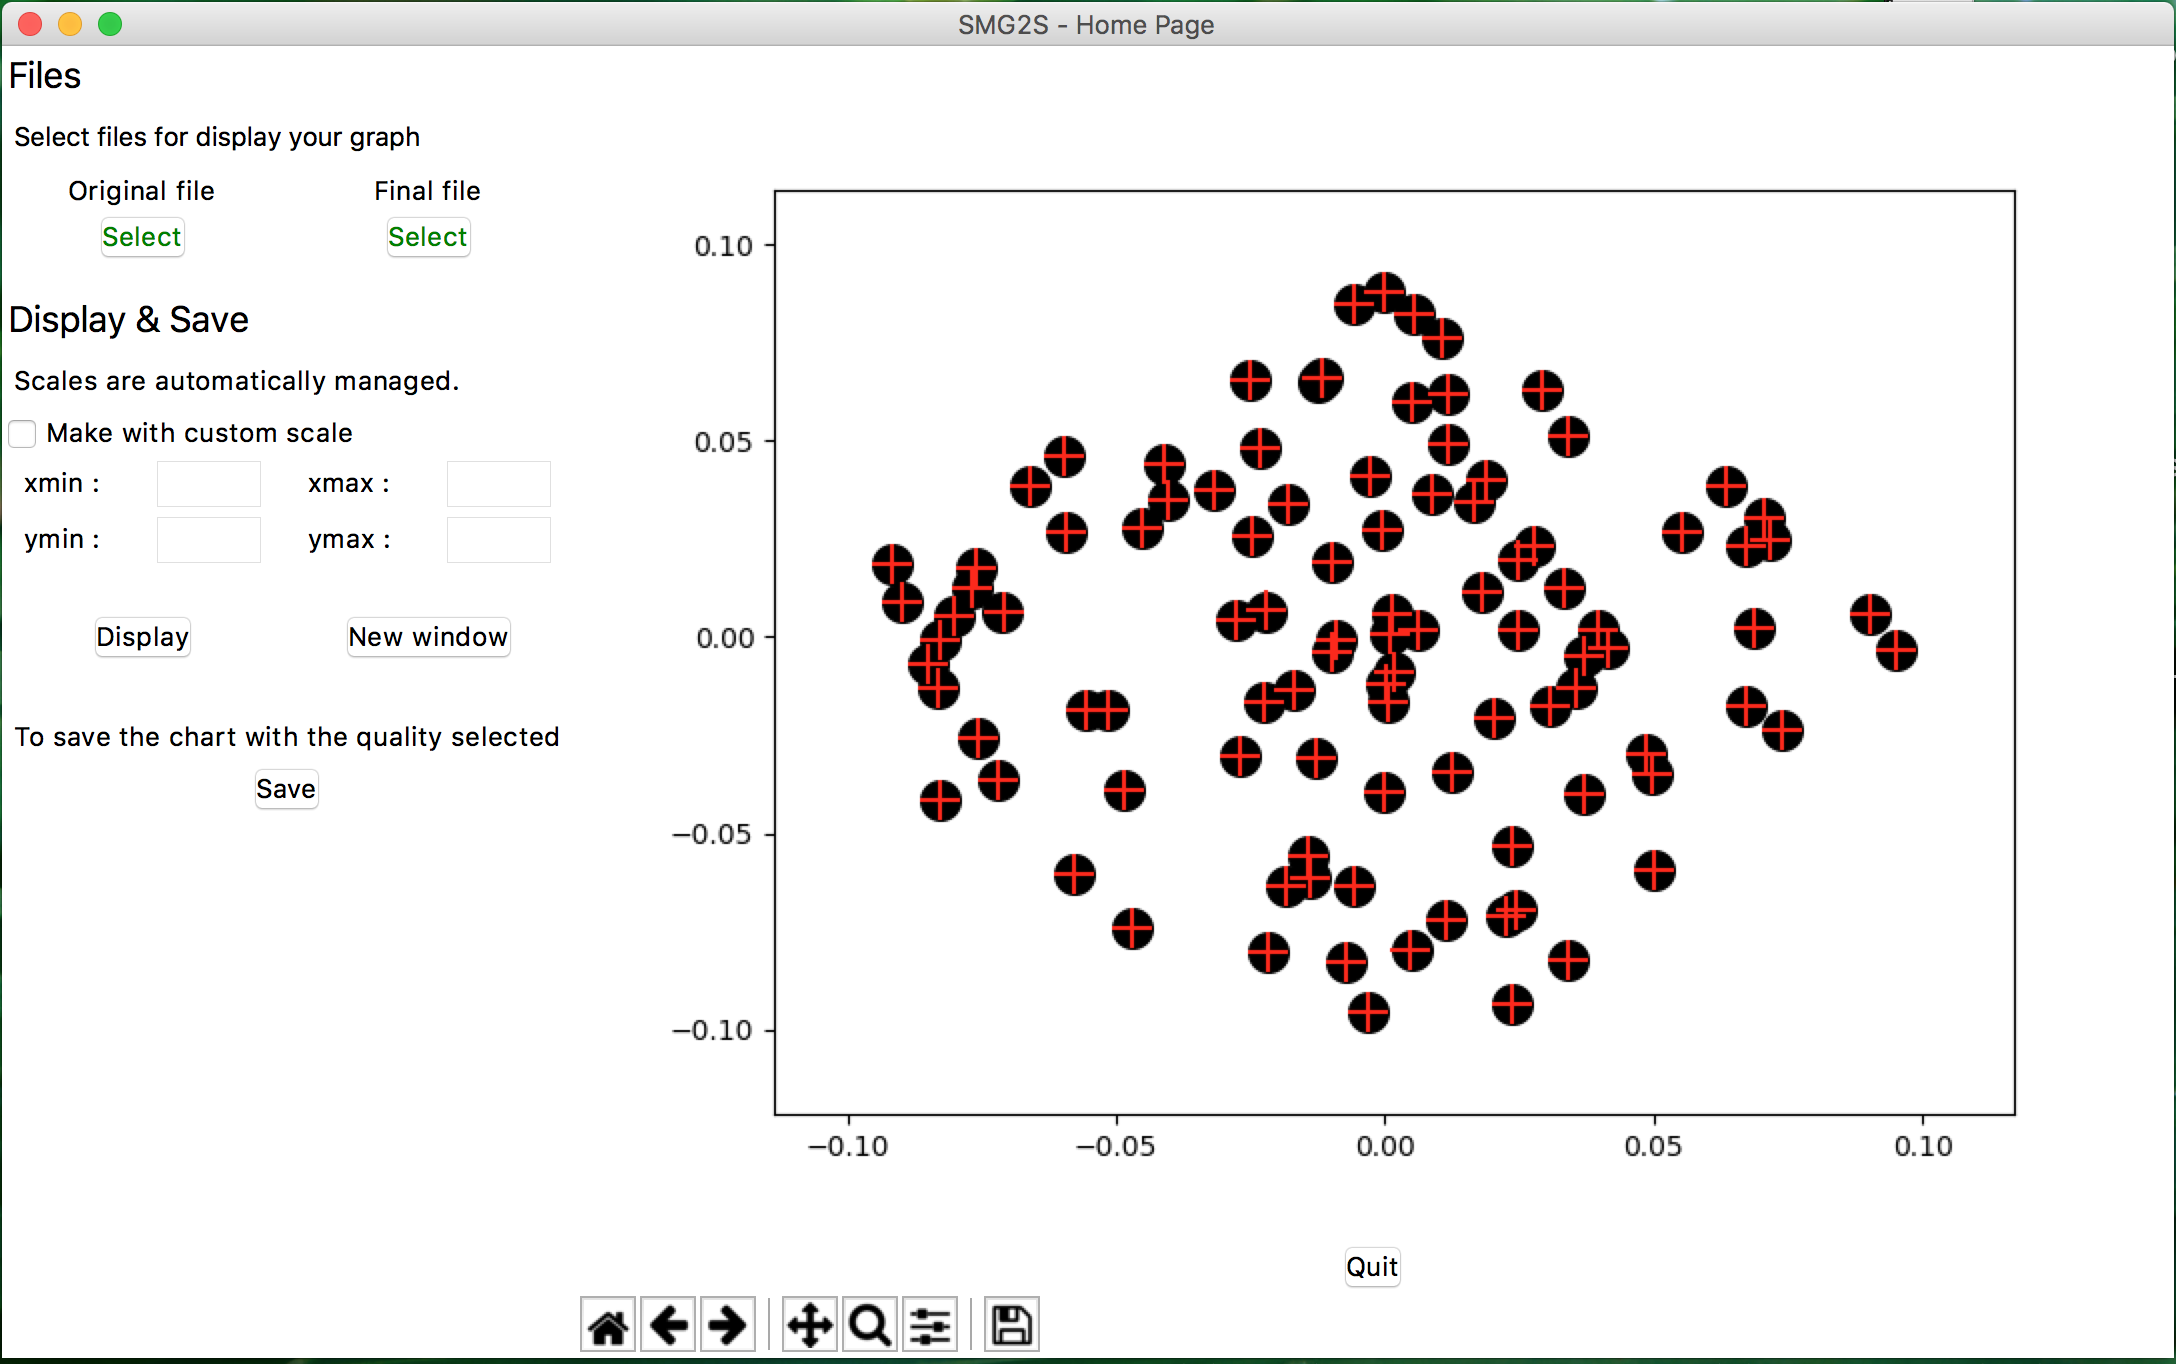
\includegraphics[width=6.2in]{fig/home_screen.png}
\end{figure}

\begin{figure}[htbp]
	\label{fig:Home Screen custom}
	\caption{Home Screen Custom}
	\centering
	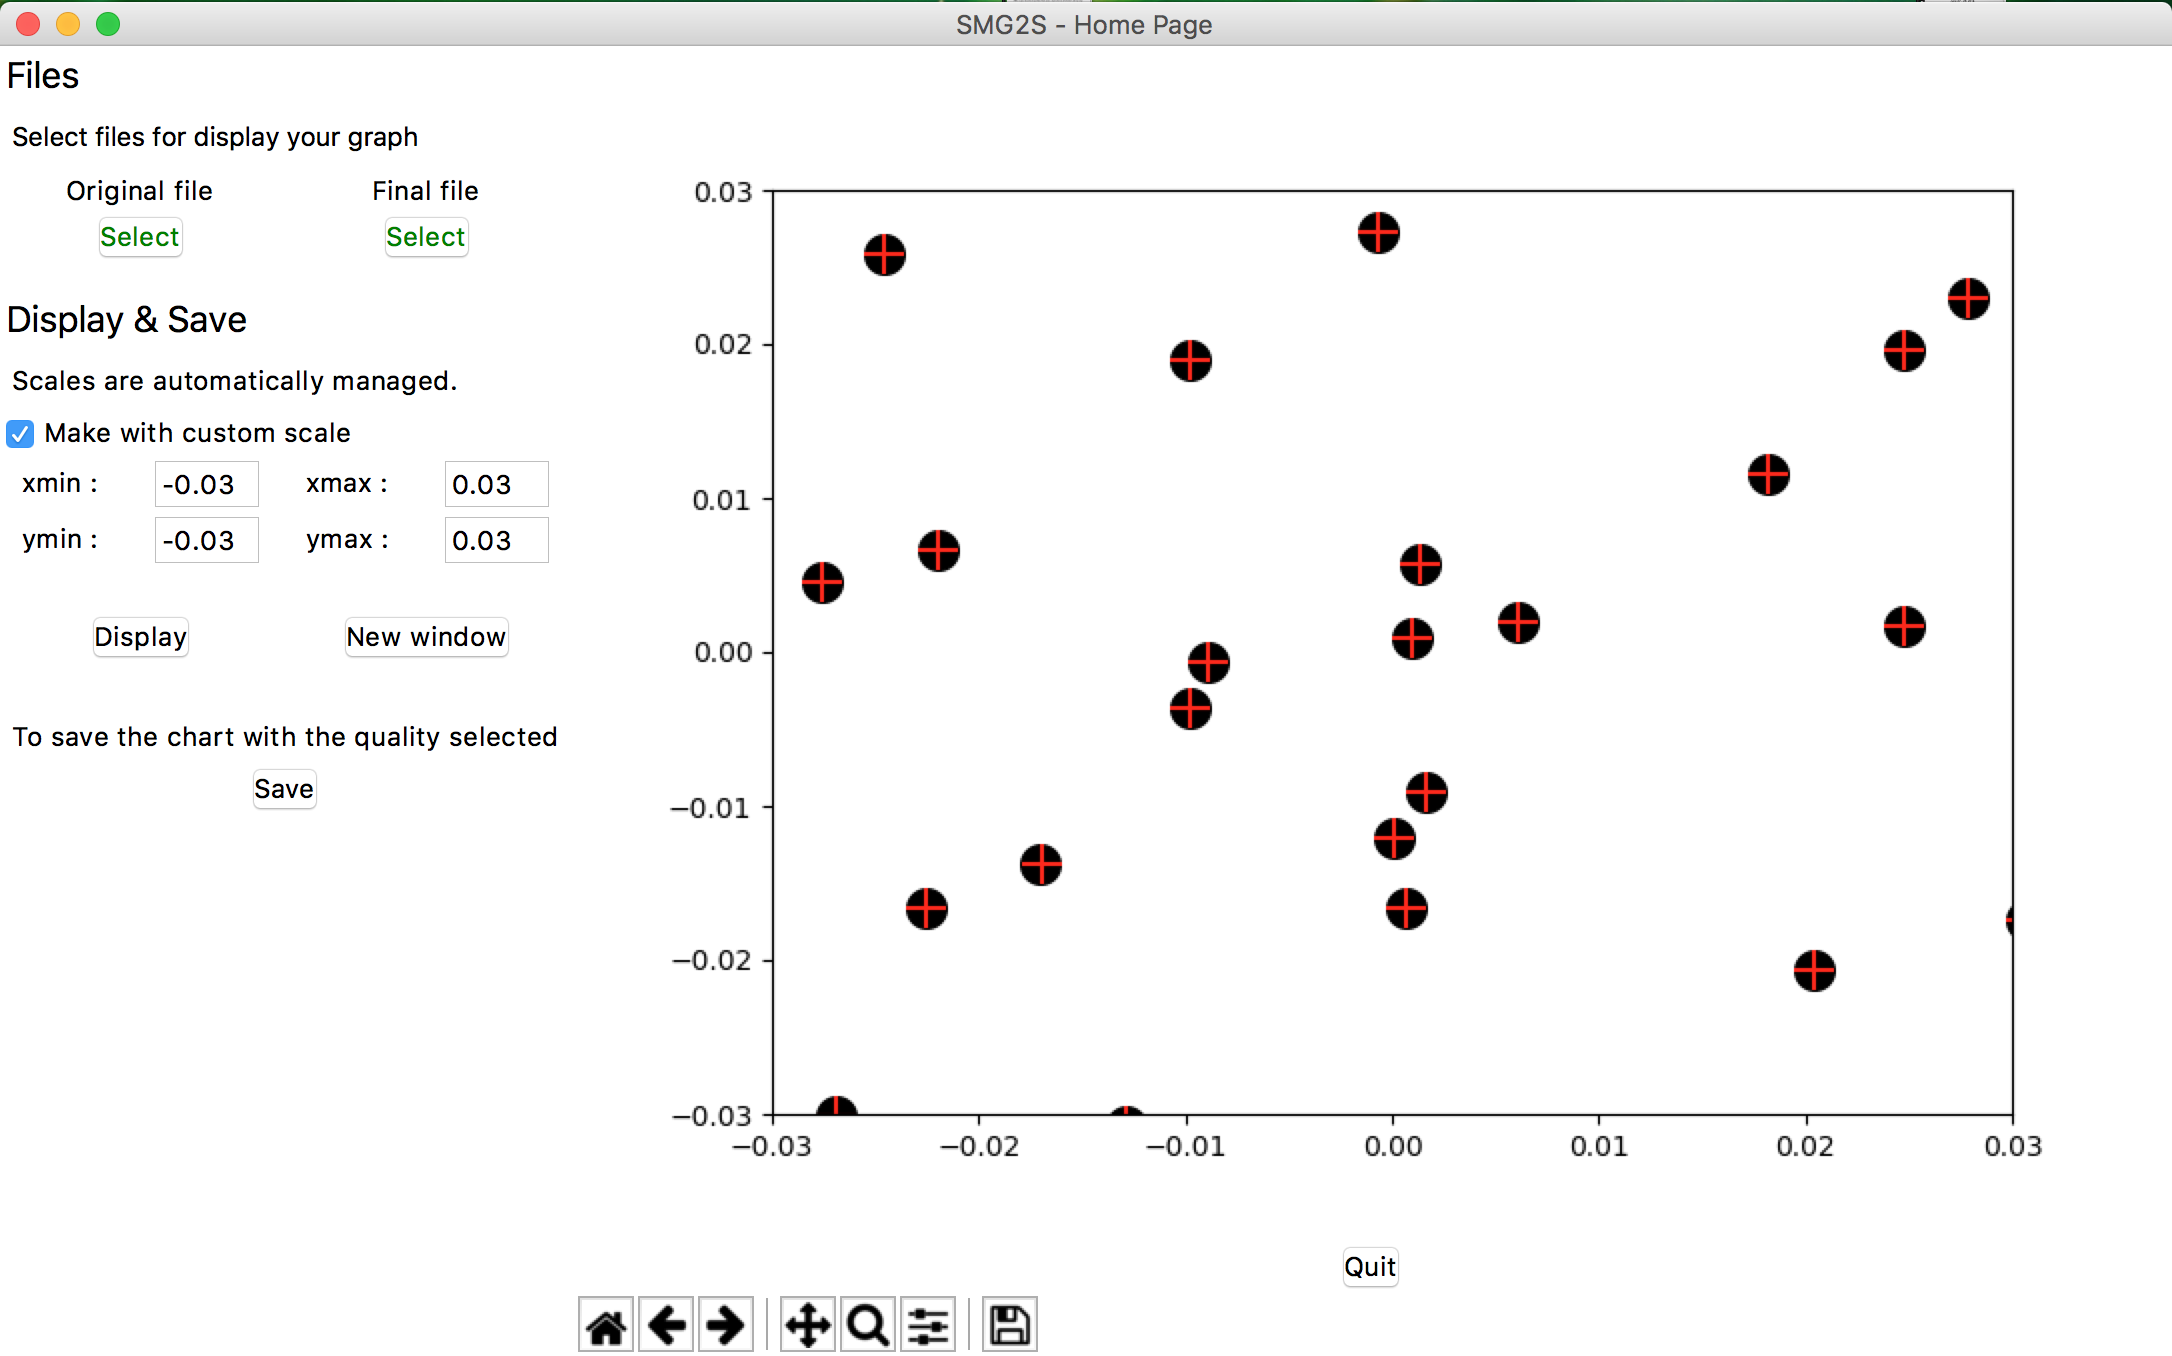
\includegraphics[width=6.2in]{fig/home_screen_custom.png}
\end{figure}


\subsection{Krylov Solvers Evaluation using SMG2S}\label{application}

SMG2S is suitable to evaluate different kinds of linear system and eigenvalue solvers. We give an example to demonstrate its workflow by evaluating the Krylov solvers. In this section, we do not mean to propose novel points on the Krylov methods, but to show the benefits of SMG2S. A class of Krylov subspace iterative methods is one of the most powerful tools to solve large and sparse linear systems. Their significant advantages such as low memory requirements and a good approximation of solution make them widely be used in applications throughout science and engineering. Convergence analysis of these methods is not only of a great theoretical importance but it can also help to answer practically relevant questions about improving their performance using the preconditioners. As we introduced in Section \ref{introduction}, the convergence of Krylov solvers depends on the spectral distribution of matrices. And most preconditioners are applied to change the spectral distribution in order to accelerate the convergence. Anyway, the spectrum has a great impact on the convergence of Krylov methods. We can use SMG2S to generate the test matrices with different spectral distributions and to study their influence on the convergence.

\begin{figure}[htbp]
	\label{fig:smg2s-convergence}
	\caption{Convergence Comparison using a matrix generated by SMG2S.}
	\centering
	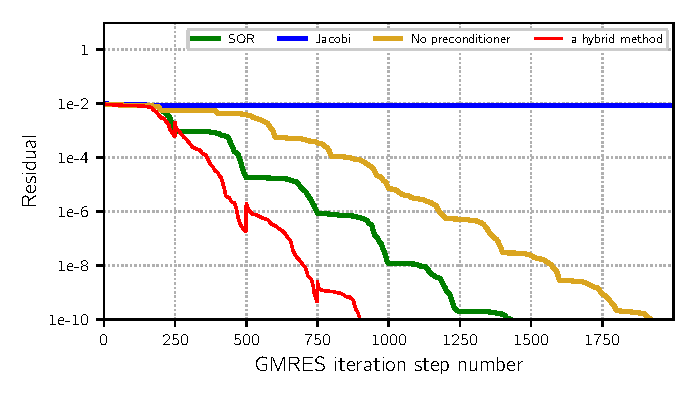
\includegraphics[width=6.2in]{fig/smg2s_convergence.eps}
\end{figure}

\begin{table*}[h]
	\caption{Krylov Solvers Evaluation by SMG2S with matrix row number = \num[round-precision=2,round-mode=figures]{100000}, convergence tolerance = \num[round-precision=2,round-mode=figures]{0.0000000001} (dnc = do not converge in  \num[round-precision=2,round-mode=figures]{80000} iterations, the solvers and preconditioners are provided by PETSc.)}
	\label{krylov}
	\centering
	\footnotesize
	\renewcommand{\arraystretch}{1.5}
	\begin{tabular}{cccccccc}
		\hline
		\textbf{Krylov Methods} & \textbf{Preconditioner} & \textbf{Case 1} & \textbf{Case 2} 
		& \textbf{Case 3} & \textbf{Case 4} & \textbf{Case 5} & \textbf{Case 6} \\ 
		\hline
		\multirow{3}{*}{GMRES} & None & 2160 & dnc
		& dnc & dnc &50773 & dnc\\ 
		\cline{2-8}
		& Jacobi& 17 & dnc & 129 & dnc &12056 & dnc\\
		\cline{2-8}
		& SOR& 3 &dnc & 4 &dnc & dnc & dnc\\
		\hline
		\multirow{3}{*}{BiCGStab} & None & 220 & 6859
		& dnc&771 &53 &dnc\\ 
		\cline{2-8}
		& Jacobi& 9& 1097 & 66 &214 & 56 &dnc\\
		\cline{2-8}
		& SOR&2 &168 & 3 & 12 & 8& dnc\\
		\hline
		\multirow{3}{*}{TFQMR} & None & 510 & dnc
		& dnc &dnc &dnc& dnc\\ 
		\cline{2-8}
		& Jacobi& 18 & dnc & 128 & dnc & dnc& dnc\\
		\cline{2-8}
		& SOR& 3&dnc &  5&22 &dnc& dnc\\
		\hline
		
	\end{tabular}
\end{table*}

\subsubsection{SMG2S workflow to evaluate Krylov Solvers}

SMG2S workflow for evaluating the solvers is shown in Fig. \ref{fig:interface}. It generates the matrix in parallel, which means that the different parts of the matrix are already distributed into the computing units of the platform. An interface can be provided to PETSc, Trilinos, and any public or personal parallel solvers. This interface can restore the distributed data into the necessary data structures of different libraries. This feature can significantly reduce the I/O of applications and improve their efficiency to evaluate the numerical methods.

\subsubsection{Experiments}

We evaluate three different restarted Krylov linear system solvers by SMG2S. The test methods include GMRES, BiCGStab (BiConjugate Gradient Stabilized method), and TFOMR (Transpose Free Quasi-Minimal Residual), with/without the basic parallel preconditioners SOR or Jacobi. In the experiments, matrices with different spectral distributions are generated by SMG2S, including the clustered, closest, conjugate eigenvalues, eigenvalues with dominant values, etc. With the interface implemented between SMG2S and PETSc, we use the parallel Krylov solvers and preconditioners provided by PETSc to do the evaluations.

Table \ref{krylov} shows iterative steps for convergence of different solvers. We can conclude that different matrices generated by SMG2S with different spectral distributions have divers convergence performance with different solvers and preconditioners. The 6 cases listed in Table \ref{krylov} are not cover much more different types of spectral distributions, and the tested preconditioners are relatively simple because it is not the main purpose of this paper. But we can say that SMG2S is a reliable tool which can be used to evaluate the different numerical methods, and in the future, we will make use of it to do more tests with different solvers and novel preconditioners and to analyze their performance with different spectral distributions.

\section{Conclusion and Pespectives}\label{conclusion}

In this chapiter, we have presented a scalable matrix generator with the given spectra and its parallel implementation on homogenous and heterogenous clusters. This method allows generating large-scale test matrices with customized eigenvalues to evaluate the influence of spectra on the linear and eigenvalue solvers targeting the large-scale platform. We have evaluated the parallel scalability and the accuracy to keep the spectra of matrices generated by this matrix generator. The experiments proved that this method has good scalability and acceptable accuracy to keep the given spectra. One more important benefit of SMG2S is that the matrices are generated in parallel, thus the data are already allocated on different processes. These distributed data can be use directly for the users to efficiently evaluate the numerical linear methods of the scientifc libraries or their personal implementation without concerning the I/O operation, whose time consumption is enormous if the matrix size is large. In future, in order to augment the bandwidth of generated matrix, a special data structure and function for the very large factorial operation should be implemented. And the interface to more scientific linear and eigenvalue solver libraries should be provided.


\clearemptydoublepage


\chapter[Unite and Conquer GMRES/LS-ERAM Method]{Unite and Conquer GMRES/LS-ERAM Method}\label{Unite and Conquer GMRES/LS-ERAM Method}

\begin{displayquote}
	
	\textsf{Facing the challenges of numerical linear algebra methods on a large-scale machine discussed in Section 3, the new programming model should be proposed with well-suited characteristics on modern architectures. These features include optimized communications, asynchronicity, diversity of natural parallelism and fault tolerance. In such numerical methods, the avoidance of operations involving synchronous communications is most important. Indeed, with a very large number of cores, the overall reductions or global synchronization are a bottleneck. Consequently, large scalar products and overall synchronization, and other operations involving communications between all cores have to be avoided. On the other hand, everywhere that is possible, asynchronicity of communications has to be promoted. Indeed, this kind of communications could allow their overlapping with computation operations inside a task and between the tasks constituting theses methods. The communication avoiding techniques could also be integrated allowing a general reduction of communications in the algorithm. The diversity of natural parallelism existing in such methods can be exploited by taking advantage of heterogeneity of targeted architectures. Fault tolerance and the ability to load balancing should be integral parts of these methods. These characteristics allow the improvement of the performance of applications built on the basis of these methods. Moreover, based on these properties, auto/smart-tuned versions of algorithms can be proposed. In this chapter, we present an asynchronous distributed and parallel Unite and Conquer GMRES/LS-ERAM (UCGLE) method to solve sparse non-Hermitian systems on large platforms. The key feature of UCGLE comparing with the classical hybrid methods using LS polynomial preconditioner \cite{essai1999heterogeneous,he2006hybrid} is its distributed and parallel asynchronous communication and the manager engine implementation among three components, which are specified for the extreme-scale supercomputing platforms. We summarize the UC approach in Section 5.1. The theoretical parts of UCGLE are given in Section 5.2. In Section 5.3, we present the distributed and parallel implementation of UCGLE, including the computing components, the manager engine, and the distributed and parallel asynchronous communications. The experimental results on different supercomputers which evaluate the convergence, the parameters, the scalability, and the fault tolerance are shown in Section 5.5.}
\end{displayquote}

\vspace{1in}
\section{Unite and Conquer approach}

In general, Unite and Conquer approach is to make collaborate several iterative methods in order to accelerate the convergence of one of them. It is important to recall that the hybrid methods defined according to this approach are particularly interesting when underlying computing platforms are constituted by parallel and/or distributed heterogeneous components. This approach is a model for the design of numerical methods by combining different computation components together to work for the same objective, with asynchronous communication among them. Unite implies the combination of different calculation components, and conquer represents different components work together to solve one problem. Different independent components with asynchronous communication can be deployed on various platforms such as P2P, cloud and the supercomputer systems. The idea of unite and conquer approach came from the article of Saad \cite{saad1984chebyshev} in 1984, where he suggested using Chebyshev polynomial to accelerate the convergence of Explicitly Restarted Arnoldi Method (ERAM) to solve eigenvalue problems. Brezinski \cite{brezinski1994hybrid} proposed in 1994 an approach for solving a system of linear equations which takes a combination of two arbitrary approximate solutions of two methods. In 2005, Emad \cite{emad2005multiple} proposed a hybrid approach based on a combination of multiple ERAMs, which showed significant improvement in solving different eigenvalue problems. In 2016, Fender \cite{fender2016leveraging} studied a variant of multiple IRAMs and generated multiple subspaces in a nested fashion in order to dynamically pick the best one inside each restart cycle.

The multiple explicitly restarted Arnoldi method is a technique based upon an ERAM with multiple projections.
This method projects an eigenproblem on a set of subspaces and thus creates a whole range of differently parameterized ERAM processes which cooperate to compute a solution of this problem efficiently. As shown in Fig. \ref{meram}, in MERAM the restarting vector of an ERAM is updated by taking into account the interesting eigeninformation obtained by the other ones. In other words, the ERAM processes of a MERAM begin with several subspaces spanned by a set of initial vectors and a set of subspace sizes. If the convergence does not occur for any of them, then the new subspaces will be defined with initial vectors updated by taking into account the intermediary solutions computed by all the ERAM processes. Each of these differently sized subspaces is defined with a new initial vector v. To overcome the storage dependent shortcoming of ERAM, a constraint on the subspace size of each ERAM is imposed. We have seen that this method accelerates the convergence of explicitly restarted Arnoldi method. The numerical experiments have demonstrated that this variant of MERAM is often much more efficient than ERAM. Fig. \ref{meram} gives an experimental results extracted from \cite{emad2005multiple}.

\begin{figure}[htbp]
	\centering
	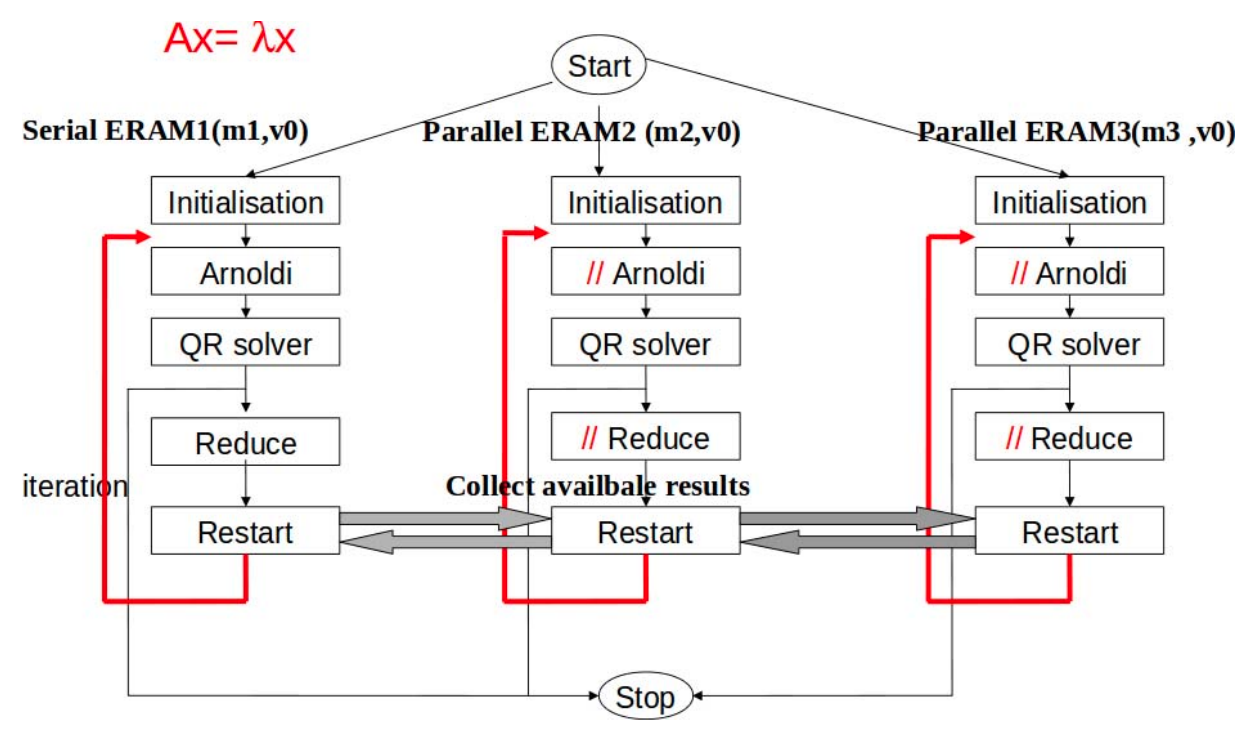
\includegraphics[width=6.2in]{fig/meram.png}
	\caption{An overview of MERAM \cite{emad2005multiple}.}
	\label{meram}
\end{figure}

\begin{figure}[htbp]
	\centering
	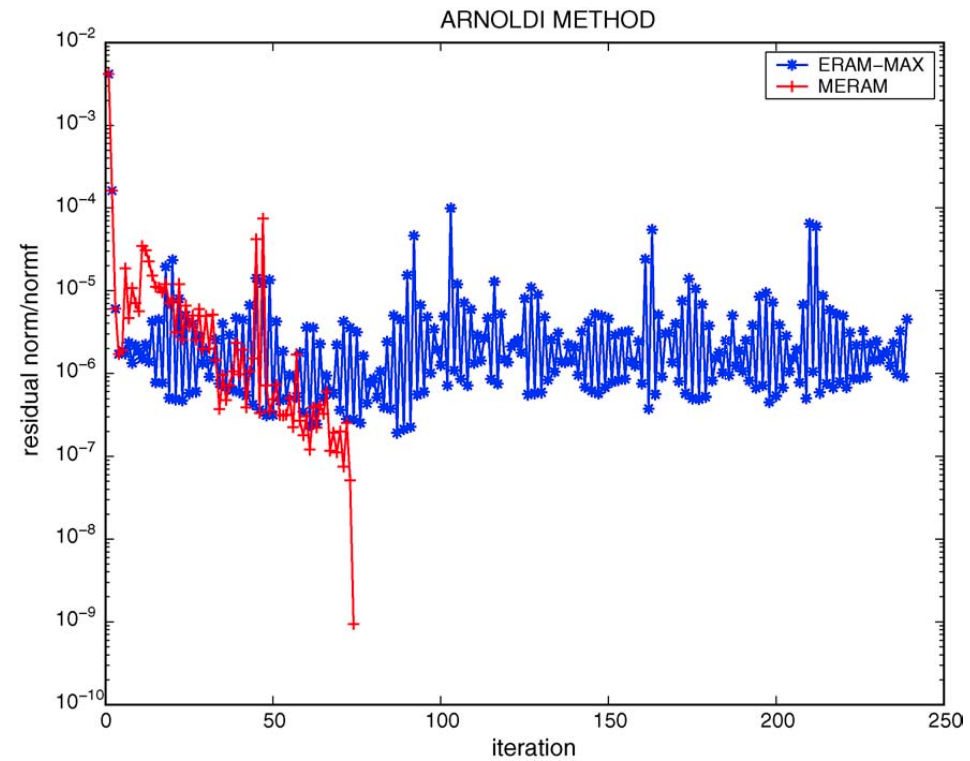
\includegraphics[width=6.2in]{fig/meram_perf.png}
	\caption{An example of MERAM: MERAM(5,7,10) vs. ERAM(10) with af 23560.mtx matrix. MERAM converges in 74 restarts, ERAM does not converge after 240 restarts \cite{emad2005multiple}.}
	\label{meram-perf}
\end{figure}

\section{Asynchronous Unite and Conquer GMRES/LS-ERAM Method}

\textcolor{red}{(Need to compare the traditional hybrid methods and UC methods, considering the goals of numerical methods on modern supercomputers that talked in Chapter 3, and explain why use polynomial preconditioning, not matrix preconditioning.)}

As shown in Chapter 3, there are three types of preconditioners to accelerate the convergence of linear solvers: 1) by preconditioning matrix; 2) by the deflation of eigenvalues/eigenvectors; 3) by the selected polynomials. When thinking about to construct a linear solver based on the \textit{Unite and Conquer approach} by combining several methods with asynchronous communications, the deflation and the polynomial preconditioning are the good candidates. It is difficult to separate the linear solver and preconditioning matrix with asynchronous communications. Thus, we select the hybrid method which is preconditioned by the least squares polynomial to construct our new model. In the conventional implementation of this method, the eigenvalues used to construct the least squares polynomials are computed by the Hessemberg matrix $H_m$ after each time restart of GMRES. In UCGLE, the linear solver, the approximation of eigenvalues and the construction of least squares polynomials are separated into three different parts. These three computing components work independently with each other and they share the necessary information by the asynchronous communications.

UCGLE method comprises mainly two parts: the first part uses the restarted GMRES method to solve the linear systems; in the second part, it computes a specific number of approximated eigenvalues, and then applies them to the Least Squares method and gets a new preconditioned residual, as a new initial vector for restarted GMRES. 

Figure \ref{fig:worflow} gives the workflow of UCGLE method with three computation components. ERAM Component and GMRES Component are implemented in parallel, and the communication among them is asynchronous. ERAM Component computes a desired number of eigenvalues, and then sends them to LS Component; LS Component uses these received eigenvalues to output a new residual vector, and sends it to GMRES Component; GMRES Component uses this residual as a new restarted initial vector for solving non-Hermitian linear systems.

\begin{figure}[htbp]
	\centering
	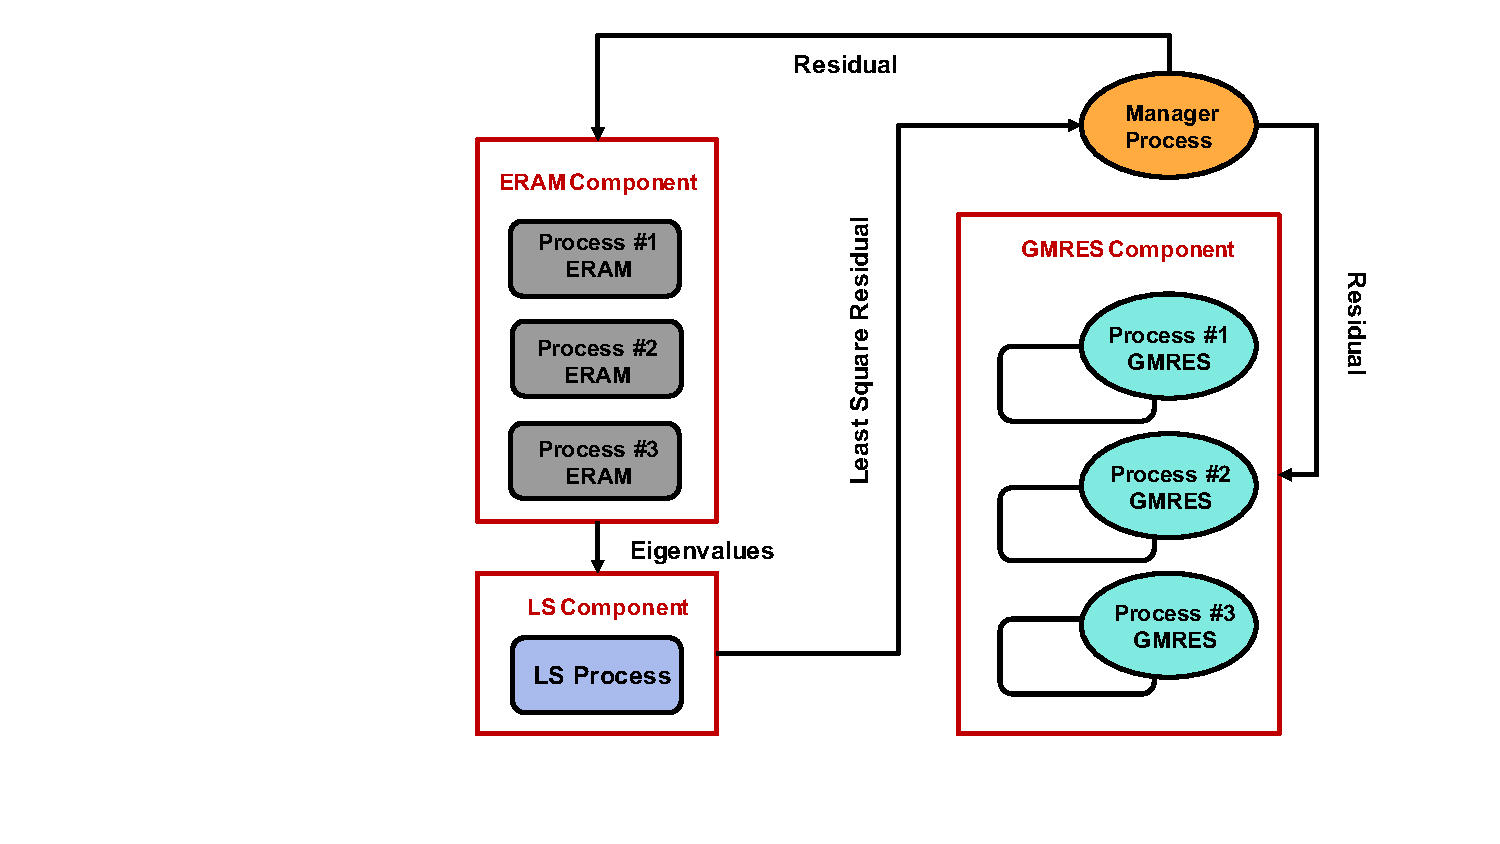
\includegraphics[width=5.2in]{fig/workflow.pdf}
	\caption{Workflow of UCGLE method's three components}
	\label{fig:worflow}
\end{figure}


\section{Distribuetd and Parallel Implementation}

This section gives the distributed and parallel implementation, including the components, the multi-level parallelism, the manager engine, and the asynchronous communications.
\subsection{Component Implementation}

This section gives the basic implementation and workflow for each component in UCGLE, and Algorithm \ref{alg:gmres/ls-a} gives the implementation of UCGLE in details.

\subsubsection{GMRES Component}

GMRES Component aims to complete the solving a linear system $Ax=b$. It takes as input an operator matrix $A$ and two vectors, $x$ the initial guess vector and $b$ the related RHS. GMRES approximates the solution starting from this initial guess vector until the exact solution is found or if a stopping criterion is met, for example, that the residual norm is below a given threshold (e.g., $||r||_2 \leq 10e^{-8}$). In practice, GMRES are restarted after $m$ steps of iterations in order to reduce the memory requirement. Before each time of restart, GMRES Component check if it receives asynchronously the LS parameters from LS Component. If received, it will provide these parameters to generate a new residual vector and use it as the restart vector, if not, GMRES will be normally restarted. Fig. \ref{gmres-component} gives the workflow of GMRES Component.

GMRES Component loads the parameters $A, m_g, x_0, b, \epsilon_g, L, s_{use}$ to solve the linear systems. At the beginning of the execution, it behaves like the basic GMRES method. When it finishes the $m^{th}$ iteration, it will check if the condition $||b-Ax_m||<\epsilon_g$ is satisfied, if yes, $x_m$ is the solution of linear system $Ax=b$, or GMRES Component will be restarted using $x_m$ as a new initial vector. A parameter $count$ is used to count the times of restart. All these processes are similar to a Restarted GMRES. However, when $count$ is an integer multiple of $L$ (number of GMRES restarts between two times preconditioning of LS), it will check if it has received the parameters $A_d, B_d, \Delta_d, H_d$ from LS Component. If yes, these parameters will be used to construct a preconditioning polynomial $P_d$, which can be used to generate a preconditioned residual $x_d$, then set the initial vector $x_0$ as $x_d$, and restart the basic GMRES, until the exit condition is satisfied.

The GMRES component has the role of solving the linear system.  We reused PETSc's GMRES resolution method and modified it to include sending and receiving data and calculating the new residual. After going through a configuration phase of the numerical method, relating to parameters as important as the size of subspace to be used, as well as the residual standard to be achieved.

\begin{figure}[htbp]
	\centering
	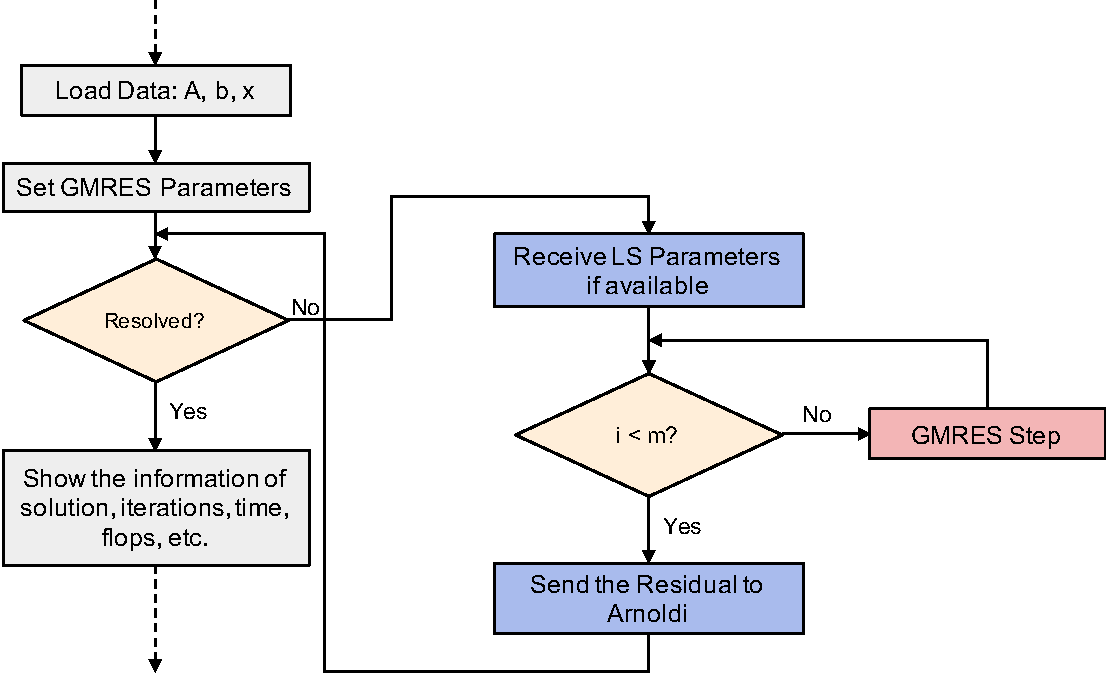
\includegraphics[width=6.2in]{fig/GMRES-component.pdf}
	\caption{GMRES Component.}
	\label{gmres-component}
\end{figure}

\subsubsection{ERAM Component}

\begin{figure}[htbp]
	\centering
	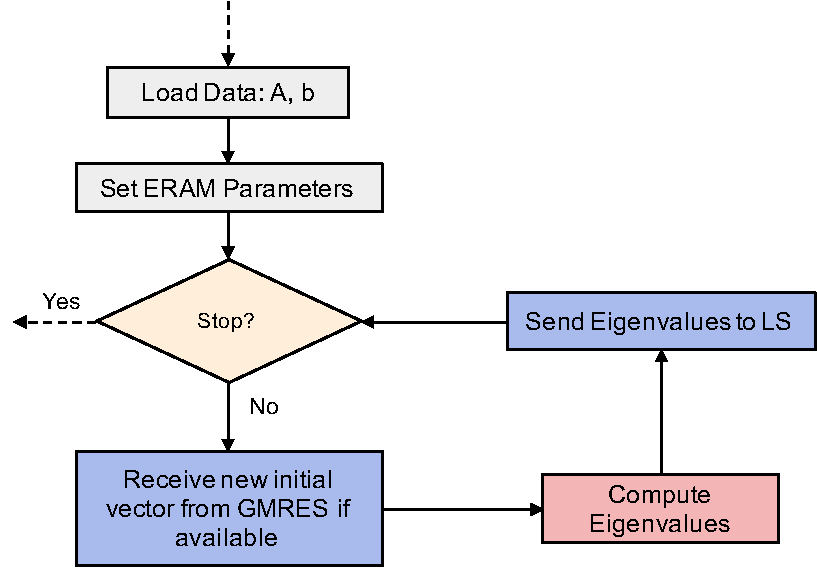
\includegraphics[width=4.8in]{fig/ERAM-component.pdf}
	\caption{ERAM Component.}
	\label{eram-component}
\end{figure}

Fig. \ref{eram-component} gives the workflow of ERAM Component. ERAM Component loads the parameters $m_a, v, r, \epsilon_a$ and the operator matrix $A$, then launches ERAM function. When it receives a new vector $X\_TMP$ from GMRES Component, this vector will be stored in ERAM Component. This vector is updated with the continuous receiving of a new one from GMRES Component. If the $r$ eigenvalues $\Lambda_r$ are approximated by ERAM Component, it will send them to LS Component, at the same time, it is able to save the eigenvalues into the local file.

\subsubsection{LS Component}

Fig. \ref{ls-component} gives the workflow of ERAM Component. LS Component won't start work until it receives the eigenvalues $\Lambda_r$ sent from ERAM Component. Then it will use them to compute the parameters $A_d, B_d, \Delta_d, H_d$, whose dimensions are related to LS parameter $d$, the Least Squares polynomial degree, and send these parameters to GMRES Component.

\begin{figure}[htbp]
	\centering
	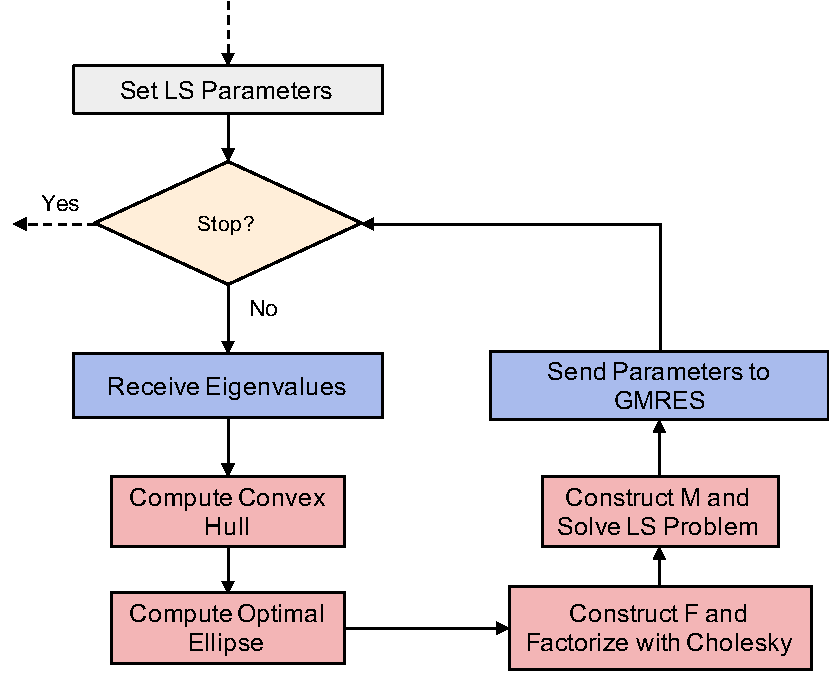
\includegraphics[width=4.8in]{fig/LS-component.pdf}
	\caption{LS Component.}
	\label{ls-component}
\end{figure}

\begin{breakablealgorithm}
	\caption{Implementation of Components}   
	\label{alg:gmres/ls-a}   
	\begin{algorithmic}[1]
		\Function{LOADERAM}{$input$: $A, m_a, \nu, r, \epsilon_a$}
		\While{exit==False}
		\State ERAM($A, r, m_a, \nu,\epsilon_a$, $output$: $\Lambda_r$)
		\State Send ($\Lambda_r$) to LS
		\If{$saveflg==TRUE$} 
		\State write ($\Lambda_r$) to file $eigenvalues.bin$\EndIf
		\If{Recv ($X\_TMP$)} 
		\State update $X\_TMP$\EndIf
		\If{Recv ($exit==TRUE$)} 
		\State Send ($exit$) to LS Component  \State stop \EndIf
		\EndWhile
		\EndFunction
		\Function{LOADLS}{$input$: $A,b, d$}
		\If {Recv($\Lambda_r$)}
		\State LS{($input$: $A,b,d,\Lambda_r$, $output$: $A_d, B_d, \Delta_d, H_d$)}
		\State Send ($A_d, B_d, \Delta_d, H_d$) to GMRES Component
		\EndIf
		\If{Recv ($exit==TRUE$)} 
		\State stop \EndIf
		\EndFunction
		
		\Function {LOADGMRES}{$input$: $A, m_g, x_0, b, \epsilon_g, L, s_{use}$, $output$: $x_m$}
		\State $count=0$
		\State BASICGMRES{($input$: $A, m, x_0,b$, $output$: $x_m$)}
		\State $X\_TMP = x_m$
		\State Send ($X\_TMP$) to ERAM Component
		\If{$||b-Ax_m||<\epsilon_g$}
		\State \Return $x_m$
		\State Send ($exit==TRUE$) to ERAM Component
		\State Stop
		\Else \If{$count \mid L$}
		\If{recv ($A_d, B_d, \Delta_d, H_d$)}
		\State $r_0=f-Ax_0$, $\omega_1 = r_0$ and $x_0=0$
		\For {$k=1,2,\cdots, s_{use}$}
		\For {$i=1, 2, \cdots, d-1$}
		\State $\omega_{i+1}=\frac{1}{\beta_{i+1}}[A\omega_i-\alpha_i\omega_i-\delta_i\omega_{i-1}]$
		\State $x_{i+1}=x_i+\eta_{i+1}\omega_{i+1}$
		\EndFor
		\EndFor
		\State set $x_0=x_d$, and GOTO 1
		\State $count++$
		\EndIf
		\Else
		\State set $x_0=x_m$, and GOTO 1
		\State $count++$
		\EndIf
		\EndIf
		\If{Recv ($exit==TRUE$)} 
		\State stop \EndIf
		\EndFunction
	\end{algorithmic}  
\end{breakablealgorithm}


\subsection{Parameters Analysis} \label{workflow}

UCGLE method is a combination of three different methods, there are a number of parameters, which have impacts on its convergence rate. We summarize these different related ones, and classify them according to their relations with different components.

\begin{enumerate}[]
	\item GMRES Component
	\begin{enumerate}[]
		\item $m_g$: GMRES Krylov Subspace size 
		\item $\epsilon_g$: absolute tolerance for  the GMRES convergence test
		\item $P_g$: GMRES core number
		\item $s_{use}$: number of times that polynomial applied on the residual before taking account into the new eigenvalues
		\item $L$: number of GMRES restarts between two times of LS preconditioning
	\end{enumerate}
	\item ERAM Component
	\begin{enumerate}[]
		\item $m_a$: ERAM Krylov subspace size
		\item $r$: number of eigenvalues required
		\item $\epsilon_a$: tolerance for the ERAM convergence test
		\item $P_a$: ERAM core number
	\end{enumerate}
	\item LS Component
	\begin{enumerate}[]
		\item $d$: Least Squares polynomial degree
	\end{enumerate}
\end{enumerate}

Suppose that the computed convex hull by Least Squares contains eigenvalues $\lambda_1,\cdots, \lambda_m$, the residual given by Least Square polynomial of degree $d-1$ is

\[
r = \sum_{i=1}^{k}\rho_i R_d(\lambda_i)u_i + \sum_{i=m+1}^{n}\rho_i R_d(\lambda_i)u_i
\]

The first part of this residual is minimized by the Least Square polynomial method using the eigenvalues inside convex hull $H_k$, and the second part is large since the related eigenvectors associated with the eigenvalues outside $H_k$. With the number of approximated eigenvalues $d$ increasing, the first part will be much closer to zero and the second part keeps enormous. The next restart process of GMRES can be still accelerated since it restarts with the combination of eigenvectors. The more eigenvalues are known, the more significant acceleration will be. The convergence comparison of UCGLE and classic GMRES is given in Fig. \ref{fig:conv}. The large peaks appear in the UCGLE curve for each time restart. It means that the residual turns to be large, and then will drop down very quickly with the acceleration of LS polynomial method.

\begin{figure}[htbp]
	\centering
	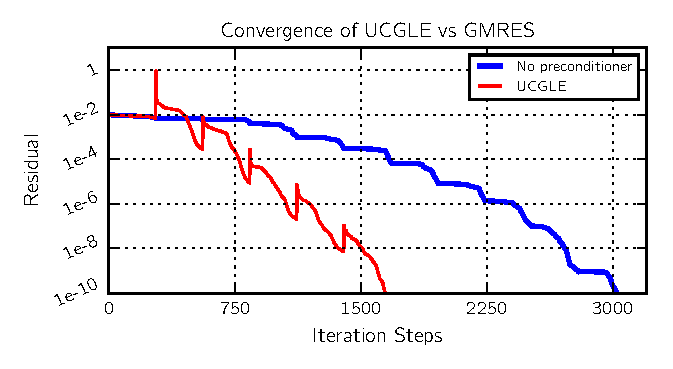
\includegraphics[width=6.2in]{fig/conv.eps}
	\caption{Convergence comparison of UCGLE method vs classic GMRES.}
	\label{fig:conv}
\end{figure}

The Algorithm \ref{alg:gmres/ls-a} shows the implementation of UCGLE's three components and their asynchronous communication in detail. 


\subsection{Multi-level Parallelism in UCGLE}

UCGLE method is a distributed parallel method which can profit both shared memory and distributed memory of computational architectures. As shown in Figure \ref{fig:glsa_mpi}, it has two levels of parallelism for distributed memory: 1) Coarse Grain/Component level: UCGLE allows the distribution of different numerical components, including the preconditioning part (LS and ERAM) and the solving part (GMRES) on different platforms or processors; 2) Medium Grain/Intra-component level, GMRES and ERAM components are both deployed in parallel; the third level for shared memory is the Fine Grain/Thread parallelism: the OpenMP thread level parallelism in CPU, or the accelerator level parallelism if GPUs or other accelerators are available. 

\begin{figure}
	\centering
	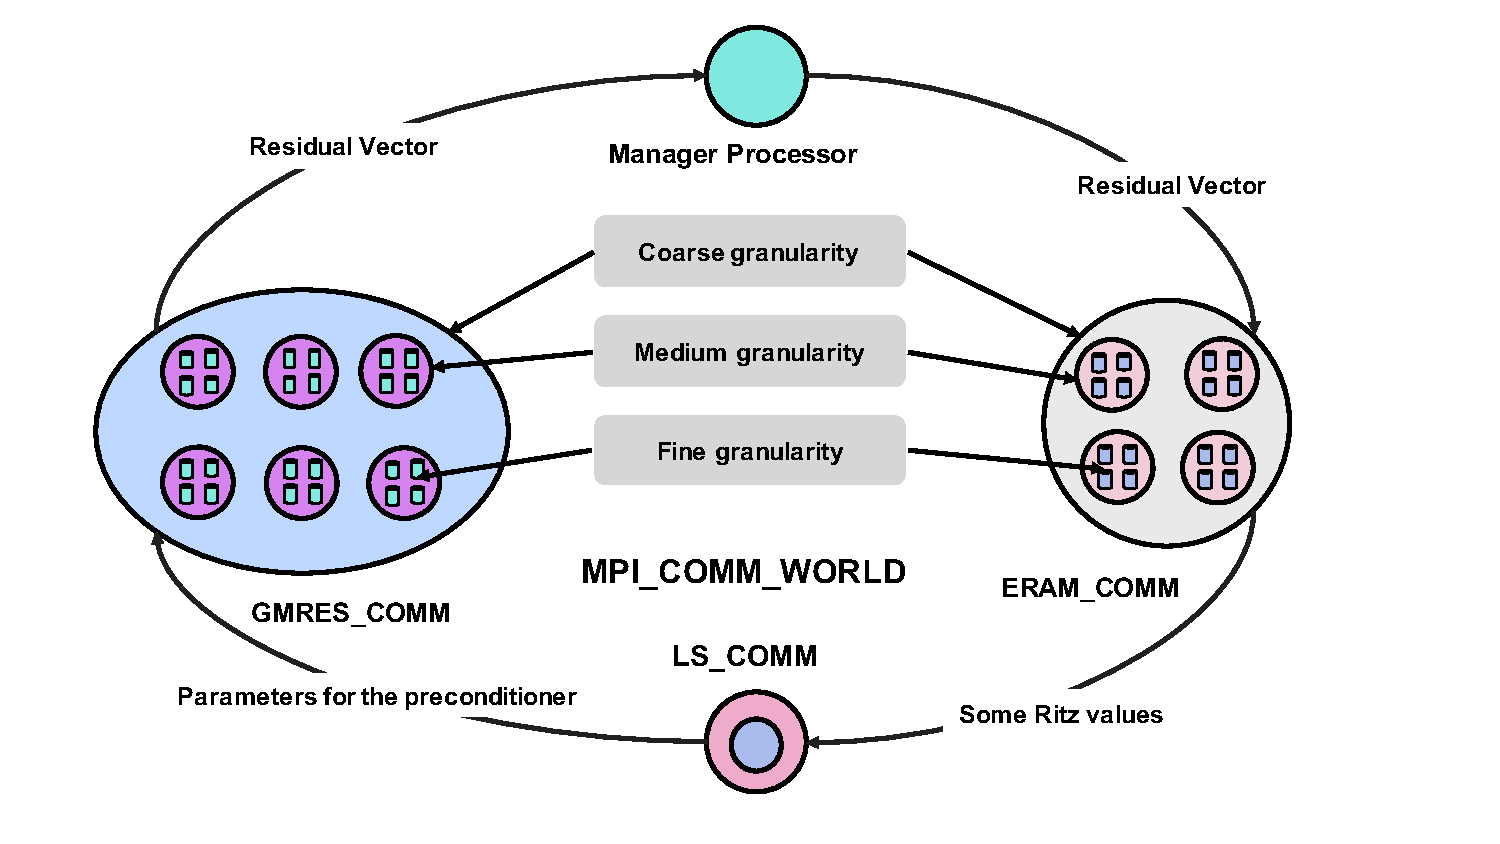
\includegraphics[width=5.2in]{fig/GLSA_MPI.pdf}
	\caption{Communication and different levels parallelism of UCGLE method}
	\label{fig:glsa_mpi}
\end{figure}

The GMRES method has been implemented by PETSc, and the ERAM method is provided by SLEPc. Additional functions have been added to the GMRES and ERAM provided by PETSc and SLEPc in order to include the sending and receiving functions of different types of data. For the implementation of LS Component, it computes the convex hull and the ellipse encircling the Ritz values of matrix $A$, which allows generating a novel Gram matrix $M$ of selected Chebyshev polynomial basis. This matrix should be factorized into $LL^T$ by the Cholesky algorithm. The Cholesky method is ensured by PETSc as a preconditioner but can be used as a factorization method. The implementation based on these libraries allows the recompilation of the UCGLE codes to adapt to both CPU and GPU architectures. The experimentation of this paper does not consider the OpenMP thread level of parallelism since the implementation of PETSc and SLEPc is not thread-safe due to their complicated data structures. The data structures of PETSc and SLEPc makes it more difficult to partition the data among the threads to prevent conflict and to achieve good performance \cite{petsc-user-ref}.


\subsection{Distributed and Parallel Manager Engine Implementation}

\subsubsection{Implementation of the Inter-component Communication Network}

From a view of asynchronous communication, the implementation of UCGLE is to establish several communicators inside of $MPI\_COMM\_WORLD$ and their inter-communication. The topology of communication among these groups is a circle shown in Figure \ref{fig:glsa_mpi}. The total number of computing units supplied by the user is thus divided into four groups according to the following distribution: $P_t$ is the total number of processes, then $P_t = P_g + P_a + P_l + P_m$, where $P_g$ is the number of processes assigned to GMRES Component, $P_a$ the number of processes to ERAM component, $P_l$ the number of processes allocated to LS Component and $P_f$ the number of processes allocated to $Manager Process$ proxy. $P_g$ and $P_a$ are greater than or equal to $1$, $P_l$ and $P_m$ are both exactly equal to $1$. LS Component is a serial component because the Least Squares polynomial method cannot be parallelized.

\begin{figure}
	\centering
	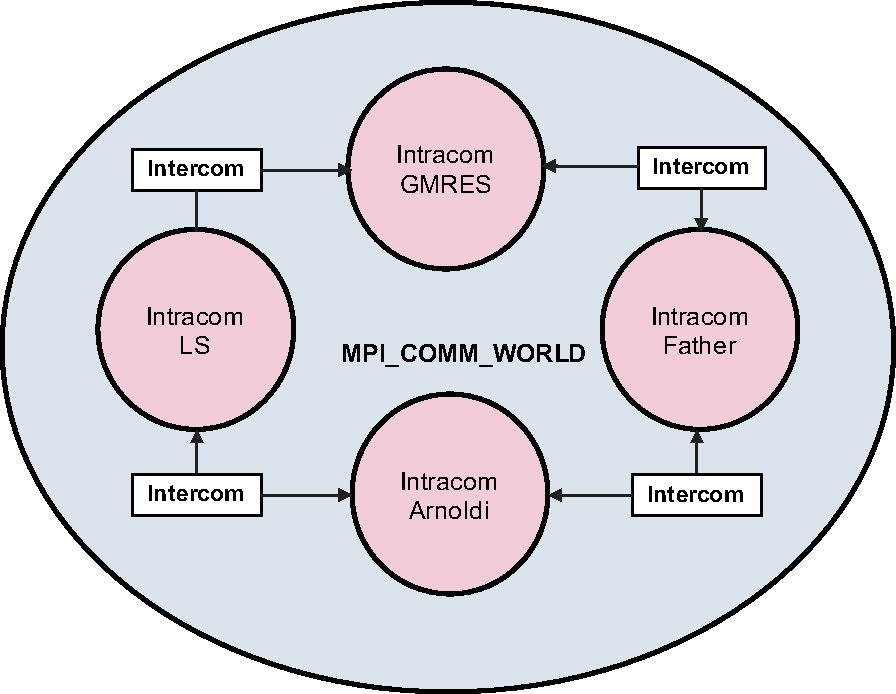
\includegraphics[width=4.2in]{fig/UCGLE_COMM_WORLD.pdf}
	\caption{Creation of Several Intra-Communicators in MPI.}
	\label{fig:ucgle_comm_world}
\end{figure}


$P_t$ is thus divided into several MPI groups according to a color code. The minimum number of processes that our program requires is $4$. We utilize the mechanism of MPI standard to support the communication of our application fully. The communication layer that does not depend on the application, this allows the replacement and scalability of various components provided.

\subsubsection{Asynchronous Communication Mechanism}

The main characteristic of UCGLE method is its asynchronous communication. But the synchronous communication takes place inside of GMRES and ERAM components. Distributed and parallel communication involves different types of exchange data, such as vectors, scalar tables, and signals among different components. When the data are sent and received in a distributed way, it is essential to ensure the consistency of data. In our case, we choose to introduce an intermediate node as a proxy to carry out only several types of exchanges and thus facilitate the implementation of asynchronous communication. This proxy is called \textit{Manager Process} as in Figure \ref{fig:glsa_mpi}. One process can fulfill all the data exchanges.

\begin{figure}
	\centering
	\includegraphics[width=6.2in]{fig/send.pdf}
	\caption{Data Sending Scheme from one group of process to the other.}
	\label{fig:send}
\end{figure}

Asynchronous communication allows each computation component to conduct independently the work assigned to it without waiting for the input data. The asynchronous data sending and receiving operations are implemented by the non-blocking communication of Message Passing Interface (MPI). Sending takes place after the sender has completed the task assigned to it. Before any prior shipment, the component checks whether several transactions are now on the way. If yes, this task will be canceled to avoid the competition of different types of sending tasks. Sent data are copied into a buffer to prevent them from being modified while sending. For the asynchronous data receiving, before starting this task, the component will check if data is expected to be received. Once the receiving buffer is allocated, the component performs the receiving of data while respecting the distribution of data globally according to the rank of sending processes. It is also essential to validate the consistency of receiving data before any use of them by the tasks assigned to the components.


\textbf{Asynchronous Sending:} The sending operation, as we described, will start by verifying if the previous sending operations are pending or not. If some operations are not finished, they are canceled so as not to be in a state where several shipments with different data are in competition. In the practical implementation, we use the MPI\_Request to track the state of an asynchronous request. Once the verification is validated, then the data to be sent will be copied to a buffer to prevent them overwritten by other work operations. Then, this data is sent to the different nodes of the other components, respecting the distribution negotiated during the initialization of the communications via the standard asynchronous sending function MPI\_Isend.

This last function is asynchronous in the sense that the data sent with this function will only be effective when the recipient (s) decide to receive them. In practice, it may be interesting to know that this is not entirely true. Indeed, the actual sending of data only occurs when the receiver or receivers are available, but also during a subsequent call to the MPI library whatever it is. Thus it may be that the sending cannot be done because the communicating nodes do not find the time to communicate. 

\begin{figure}
	\centering
	\includegraphics[width=6.2in]{fig/recv.pdf}
	\caption{Data Receiving Scheme from one group of process to the other.}
	\label{fig:recv}
\end{figure}

\textbf{Asynchronous Receiving:} In the context of send-and-receive communication mechanisms, the sending operation is often the most difficult to implement because it requires a synchronization point. As far as we are concerned, we have hidden this synchronization point thanks to an input verification step. Indeed, we have chosen to implement a test function before proceeding with asynchronous reception instead of going through a purely asynchronous reception function. The data input test is done via the MPI\_Iprobe function and the MPI\_Recv reception. The latter is blocking or synchronous, that is, once called the computation node will wait for data to be received before returning to the calling function. 

At first glance, it would seem wiser to go through the non-blocking reception function MPI\_Irecv, but in practice, this function requires to know in advance the size of the data that will be received, which is not the case in the case where our components exchange tables of scalars. Indeed, the component Arnoldi goes throughout its task, calculate more and more eigenvalues, more and more precise. In advance, it is not possible to know the number of eigenvalues that will be obtained, in fact, impossible to predict the size of the input buffer. Also, we made a choice to work with a dynamic reception buffer. In our implementation, this one is allocated thanks to the information provided by the operation MPI\_Get\_count using structure MPI\_Status filled in by the function MPI\_Iprobe.

Also, apart from this difference, our reception mechanism is fundamentally similar to the MPI\_Irecv function in that it only receives data if it is available. In our case we also do not receive data if they are not available, the component to continue its task in case they were not. 

In addition to having reimplemented MPI's asynchronous receive mechanism, we integrated a mechanism for checking the consistency of the received data. In order to allow different independent groups of compute nodes (our components), we have used the tools that are the intracommunicators and inter-communicators MPI (see explanations in 5.2.3.1). The problem of this type of implementation (at the same time there is no other possible, at least without falling into the experimental unstable) is that it does not allow collective communications between the different nodes of two communicating groups. In fact, the communications between groups of nodes (or components) pass through the intercommunication that only allow collective communications between those between the master of a group and the set of nodes of the other. This is therefore quite limiting when the goal (ours) is to carry out entirely collective communications, that is to say to allow all the nodes of a group to communicate with all the nodes of another group. This is what we have completed through our implementation of the sending and receiving mechanisms. The real problem is as to the coherence of the received data.

Indeed, even if we go through the proxy to facilitate communication control, data consistency must be checked before any prior use. For example, take the case of a vector. If a vector is partially received, it can not be used, and if it was the case, we could witness a disaster from a numerical point of view. Also, to avoid this kind of pitfall, we have integrated a validation mechanism that will check that the received data are consistent before they are used. The consistency check is conveniently performed by comparing the total size of the data received by each component node against the size of the data to be received at all. If this is consistent, then the reception buffer data is placed in the working memory of each node of the receiving component.

\subsubsection{Implementation for Hetergeneous Platforms with Multi-GPU}

\textcolor{red}{TO DO}

\section{Experiment and Evaluation}

\subsection{Hardware Platforms}

We test its convergence acceleration, fault tolerance and scalability on the large-scale platforms. UCGLE method has been installed on the supercomputer \textit{Tianhe-2}, which is installed at the National Super Computer Center in Guangzhou of China. It is a heterogeneous system made of Intel Xeon CPUs and Intel Knights Corner (KNC), with 16000 compute nodes in total. Each node composes 2 Intel Ivy Bridge 12 cores @ 2.2 GHz. In this article, we do not test UCGLE with KNC on \textit{Tianhe-2} since PETSc do not support it with good performance.

\subsection{Parameters Evaluation}

\subsubsection{Test Parameters Setup}

\begin{itemize}
	\item \textbf{Krylov subspace size for GMRES }
	\item \textbf{LS applied times: }
	\item \textbf{LS Frequence:}
\end{itemize}

\begin{itemize}
	\item \textbf{Number of eigenvalues: }
\end{itemize}

\begin{itemize}
	\item \textbf{LS polynomial degree: }
\end{itemize}

\subsubsection{Test Matrix Suite: }

\textbf{Matrices from Matrix Market Collections: }
\begin{table}[htbp]
	\renewcommand{\arraystretch}{1.4}
	\small	
	\caption{Test Matrix from Matrix Market Collection.}
	\label{testmatrixforparameters}
	\centering
	\begin{tabular}{c|c|c|c}
		\toprule
		Matrix  & Size & $s$ NNZ & $s$ Domain\\
		\midrule
		utm300  & $300$ & $3155$ &$\mathbb{R}$ \\
		utm1700b & $1700$ & $21509$  & $\mathbb{R}$ \\
		pde2961 & $2961$ & $14585$& $\mathbb{R}$ \\
		young4c & $841$ & $4089$& $\mathbb{C}$ \\
		\bottomrule
	\end{tabular}
\end{table}

\textbf{Matrices generated by SMG2S: }

\subsubsection{Experiments}

\textbf{Krylov subspace size: }

\iffalse
\begin{figure}[htbp]
	\centering
	\includegraphics[width=6.2in]{fig/conv2.eps}
	\caption{Convergence comparison of UCGLE method vs classic GMRES.}
	\label{fig:krylovsubspace}
\end{figure}
\fi

\textbf{LS applied times: }

\iffalse
\begin{figure}[htbp]
	\centering
	\includegraphics[width=6.2in]{fig/conv2.eps}
	\caption{Convergence comparison of UCGLE method vs classic GMRES.}
	\label{fig:Lsappliedtime}
\end{figure}
\fi

\textbf{LS Frequence:}

\iffalse
\begin{figure}[htbp]
	\centering
	\includegraphics[width=6.2in]{fig/conv2.eps}
	\caption{Convergence comparison of UCGLE method vs classic GMRES.}
	\label{fig:Lsfreq}
\end{figure}
\fi

\textbf{Number of eigenvalues: }

\iffalse
\begin{figure}[htbp]
	\centering
	\includegraphics[width=6.2in]{fig/conv2.eps}
	\caption{Convergence comparison of UCGLE method vs classic GMRES.}
	\label{fig:vals}
\end{figure}
\fi

\textbf{LS polynomial degree: }

\begin{figure}[htbp]
	\centering
	\includegraphics[width=6.2in]{fig/conv2.eps}
	\caption{Convergence comparison of UCGLE method vs classic GMRES.}
	\label{fig:lsdegree}
\end{figure}

\subsection{Convergence Evaluation}

We have selected four test matrices generated by SMG2S using different given spectra to evaluate the convergence speedup of UCGLE method. The first test matrix $MEG1$ and the second matrix $MEG2$ are all generated randomly inside an annulus with different scale which is symmetric to the real axis in complex plane. The size of $MEG1$ is \num[round-precision=2,round-mode=figures]{18000000}, and the size of $MEG2$ is \num[round-precision=4,round-mode=figures]{10240000}. The convergence of UCGLE is compared with 1) the restarted GMRES without preconditioning, 2) restarted GMRES with Jacobi preconditioner, 3) restarted GMRES with SOR preconditioner. We select the Jacobi and SOR preconditioners for the experimentations because they are well implemented in parallel by PETSc. The GMRES restarted parameter for $MEG1$, $MEG2$, $MEG3$ and $MEG4$ are respectively 250, 280, 30 and 40.

\begin{table}[!t]
	\renewcommand{\arraystretch}{1.2}
	\caption{Test matrices information}
	\label{matget}
	\centering
	\begin{tabular}{|c|c|c|c|}
		\hline
		Matrix Name& n & nnz & Matrix Type\\
		\hline
		$matLine$  & \num[round-precision=2,round-mode=figures]{18000000} & \num[round-precision=2,round-mode=figures]{28823000} & non-Symmetric\\
		\hline
		$matBlock$  & \num[round-precision=2,round-mode=figures]{18000000} & \num[round-precision=2,round-mode=figures]{192160000} & non-Symmetric\\
		\hline
		$MEG1$ & \num[round-precision=4,round-mode=figures]{10240000} & \num[round-mode = places, scientific-notation = fixed, fixed-exponent = 9,round-precision = 2]{7270272000} & non-Hermitian\\
		\hline
		$MEG2$ & \num[round-precision=2,round-mode=figures]{5120000} & \num[round-mode = places, scientific-notation = fixed, fixed-exponent = 9,round-precision = 2]{3635136000} & non-Hermitian\\
		\hline
	\end{tabular}
\end{table}


Fig \ref{fig:conv1}, Fig \ref{fig:conv2}, Fig \ref{fig:conv3} and Fig \ref{fig:conv4} present respectively the convergence experiments of $MEG1$, $MEG2$, $MEG1$ and $MEG2$. The numbers of iteration steos for convergence are given in Table \ref{iterations}. Obviously, UCGLE method has spectacular acceleration on the convergence for both of them over the conventional preconditioners. It has almost two times of acceleration than the SOR preconditioned GMRES. The SOR preconditioned GMRES is already better than the Jacobi preconditioned GMRES and GMRES without preconditioning for the test matrices.

\begin{figure}[htbp]
	\centering
	\includegraphics[width=6.2in]{fig/convergence1.eps}
	\caption{$MEG1$: convergence comparison of UCGLE method vs conventional GMRES}
	\label{fig:conv1}
\end{figure}

\begin{figure}[htbp]
	\centering
	\includegraphics[width=6.2in]{fig/convergence2.eps}
	\caption{$MEG2$: convergence comparison of UCGLE method vs conventional GMRES}
	\label{fig:conv2}
\end{figure}

\begin{figure}[htbp]
	\centering
	\includegraphics[width=6.2in]{fig/convergence3.eps}
	\caption{$MEG3$: convergence comparison of UCGLE method vs conventional GMRES}
	\label{fig:conv3}
\end{figure}

\begin{figure}[htbp]
	\centering
	\includegraphics[width=6.2in]{fig/convergence4.eps}
	\caption{$MEG4$: convergence comparison of UCGLE method vs conventional GMRES}
	\label{fig:conv4}
\end{figure}

\begin{table*}[htbp]
	\footnotesize
	\renewcommand{\arraystretch}{1.2}
	\caption{Summary of iteration number for convergence of $4$ test matrices using SOR, Jacobi, non preconditioned GMRES,UCGLE\_FT(G),UCGLE\_FT(G) and UCGLE: red $\times$ in the table presents this solving procedure cannot converge to accurate solution (here absolute residual tolerance \num[round-precision=2,round-mode=figures]{0.0000000001} for GMRES convergence test) in acceptable iteration number ($20000$ here).}
	\label{iterations}
	\centering
	\begin{tabular}{*{7}{c}}
		\toprule
		Matrix Name& SOR & Jacobi & No preconditioner & UCGLE\_FT(G) &UCGLE\_FT(G) & UCGLE \\
		\midrule
		$MEG1$  & 1430 & \textcolor{red}{$\times$} & 1924 & 995 & 1073 & \cellcolor{yellow}900\\
		
		$MEG2$  & 2481 & 3579 & 3027 & 2048 & 2005 & \cellcolor{yellow}1646\\
		
		$MEG3$ & 217 & 386 & 400 & 81 & 347 & \cellcolor{yellow}74\\
		
		$MEG4$ & 750 & \textcolor{red}{$\times$} & \textcolor{red}{$\times$} & 82 & \textcolor{red}{$\times$} & \cellcolor{yellow}64\\
		\bottomrule
	\end{tabular}
\end{table*}

\subsection{Scalability Evaluation}

\textcolor{red}{This section should be rewritten to compare the scaling perfomance both on Tianhe-2 and Romeo. }

For the resolution of large-scale linear systems on the modern supercomputing platforms, the main concern of the conventional preconditioned Krylov methods is the cost of the global communication and synchronization
overheads. We select the test matrix $MEG2$ for the scalability evaluation. The average time cost per iteration of these methods is computed by a fixed number of iterations. Time per iteration is suitable for demonstrating scaling behavior.

\begin{figure}[t]
	\centering
	\begin{tabular}{cc}
		\includegraphics[width=.48\linewidth]{fig/scalable.eps}
		&\includegraphics[width=.48\linewidth]{fig/scalable_complet.eps} \\[\abovecaptionskip]
		\small (a)& (b) 
	\end{tabular}
	\caption{Scalability per iteration comparison of UCGLE with GMRES with or without preconditioners on Tianhe-2.}\label{fig:myfig}
\end{figure}

\begin{figure}[t]
	\centering
	\begin{tabular}{cc}
		\includegraphics[width=.48\linewidth]{fig/scalable_romeo.eps}
		&\includegraphics[width=.48\linewidth]{fig/scalable_complet_romeo.eps} \\[\abovecaptionskip]
		\small (a)& (b) 
	\end{tabular}
	\caption{Scalability per iteration comparison of UCGLE with GMRES with or without preconditioners on ROMEO.}\label{fig:myfig2}
\end{figure}

For the evaluation of UCGLE on the homogeneous cluster, the core number of GMRES Component is set respectively to be 24, 48, 96, 192, 384, 768, and both the core number of LS Component and Manager Component is 1. ERAM Component should ensure to supply the approximated eigenvalues in time for each time restart of GMRES Component. Thus we select the core number is respectively 16, 32, 64, 128, 256, 512 referring to different GMRES Component core number. The GMRES core number of conventional GMRES is equal to the one of GMRES Component in UCGLE.

In Fig. \ref{fig:myfig} (a), we can find that these methods have good scalability with the augmentation of computing units except the SOR preconditioned GMRES. The classic GMRES has the smallest time cost per iteration. The Jacobi preconditioner is the simplest preconditioning form for GMRES, and its time cost per iteration is similar to the classic GMRES. The GMRES with SOR preconditioner has the largest time cost per iteration since SOR preconditioned GMRES has the additional matrix-vector and matrix-matrix multiplication operations in each step of the iteration. These operations have global communication and synchronization points. The communication overhead makes the SOR preconditioned GMRES more easily lose its good scalability with the augmentation of computing unit number. There is not much difference between the time cost per iteration of classic GMRES and UCGLE with the help of the asynchronous communication implementation of UCGLE method. Since the resolving part and preconditioning part of UCGLE work independently, its global communication and synchronize points is similar to the classic GMRES without preconditioning. That is the benefits UCGLE's asynchronous communication. 

Since UCGLE requires additional computing units for the master, LS Component and especially ERAM Component, it is necessary to compare UCGLE with other methods when the total computing resource number of UCGLE and other methods keeps the same. Thus we test also the matrix $MEG2$ using conventional methods with the computing unit number to be 38, 74, 146, 290, 578, 1154. The performance comparison is given in Fig. \ref{fig:myfig} (b). We can find that if the computing resource number is small, the time per iteration of classic and conventional preconditioned GMRES is much better than UCGLE since the latter allocates extra computing resources for other components. With the augmentation of computing resources, the scalability of the SOR preconditioned GMRES trends to be bad, and the average time cost per iteration of UCGLE method tends to be better than the SOR preconditioned GMRES with good scalability. Although the scalability of classic and Jacobi is good, and their time per iteration is smaller than UCGLE, but since UCGLE can accelerate the convergence of solving linear systems, thus better performance can be expected.


\subsection{Fault Tolerance Evaluation}

The fault tolerance of UCGLE is studied by the simulation of the loss of either GMRES or ERAM Components. UCGLE\_FT(G) in Fig. \ref{fig:conv1}, Fig. \ref{fig:conv2}, Fig. \ref{fig:conv3} and Fig. \ref{fig:conv4} represents the fault tolerance simulation of GMRES, and UCGLE\_FT(E) implies the fault tolerance simulation of ERAM. 

The failure of ERAM Component is simulated by fixing the execution loop number of ERAM algorithm, in this case, ERAM exits after a fixed number of solving procedures. We mark the ERAM fault points of the two test matrices in Fig. \ref{fig:conv1}, Fig. \ref{fig:conv2},  Fig. \ref{fig:conv3} and Fig. \ref{fig:conv4} : respectively $500$, $560$, $60$ and $30$ iteration step for each case. The UCGLE\_FT(E) curves of the experimentations show that GMRES Component will continue to resolve the systems without LS acceleration. Table \ref{iterations} shows that the iteration number for convergence of UCGLE\_FT(E) is greater than the normal UCGLE method but less than the GMRES method without preconditioning.

The failure of GMRES Component is simulated by setting the allowed iteration number of GMRES algorithm to be much smaller than the needed iteration number for convergence. The values of these cases are respectively $600$, $700$, $70$ and $48$. They are also marked in Fig. \ref{fig:conv1}, Fig. \ref{fig:conv2}, Fig. \ref{fig:conv3} and Fig. \ref{fig:conv4}. We can find that after the quitting of GMRES Component without the finish of its task, ERAM computing units will automatically take over the jobs of GMRES component. The new GMRES resolving procedure will use the temporary solution $x_m$ as a new restarted initial vector received asynchronously from the previous restart procedure of GMRES Component before its failure. In this case, ERAM Component no longer exists. Thus the resolving task can be continued as the classic GMRES without LS preconditioning. In  Fig. \ref{fig:conv1}, Fig. \ref{fig:conv2}, Fig. \ref{fig:conv3} and Fig. \ref{fig:conv4}, we can find the difference between UCGLE\_FT(E) and UCGLE\_FT(G). In UCGLE\_FT(G), the new GMRES Component takes $x_m$ of previous restart procedure. Thus it will repeat the iteration steps of previous restart iterations until the failure of GMRES. Another fact of UCGLE\_FT(G) which cannot be concluded, but can be easily obtained, is that the resolving time will be different if the computing unit numbers of previous GMRES and ERAM Components are different.


\section{Conclusion}

\clearemptydoublepage

\chapter{UCGLE for Linear Systems with Sequences of Right-hand-sides}\label{UCGLE for Linear Systems with Sequences of Right-hand-sides}

\begin{displayquote}
	\textsf{Many problems in science and engineering often require to solve a long sequence of large-scale non-Hermitian linear systems with different Right-hand sides (RHSs) but a unique operator. Efficiently solving such problems on extreme-scale platforms requires the minimization of global communications, reduction of synchronization points and promotion of asynchronous communications. Unite and Conquer GMRES/LS-ERAM (UCGLE) method presented in the last chapter is a suitable candidate with the reduction of global communications and the synchronization points of all computing units. In this chapter, we extend both the mathematical model and the implementation of UCGLE method to adapt to solve sequences of linear systems. The eigenvalues obtained in solving previous linear systems by UCGLE can be recycled, improved on the fly and applied to construct a new initial guess vector for subsequent linear systems, which can achieve a continuous acceleration to solve linear systems in sequence. Numerical experiments using different test matrices to solve sequences of linear systems on supercomputer Tianhe-2 indicate a substantial decrease in both computation time and iteration steps when the approximate eigenvalues are recycled to generate the initial guess vectors.}
\end{displayquote}

\vspace{0.6in}

\section{Demand to Solve Linear Systems in Sequence}

We consider the solution of a long sequence of general linear systems 

\begin{equation}
Ax^{(i)}=b^{(i)}, i=1,2,\cdots
\end{equation}

where $A \in \mathbf{C}^{n\times n}$ is a fixed matrix, and the right-hand side $b^{i} \in \mathbf{C}^n$ which changes from one system to another. Moreover, these systems are typically not available simultaneously. Many scientific applications require the resolution this kind of sequent linear systems, such as the finite element analysis in modeling fatigue \cite{newman1976finite, gullerud2001mpi,sukumar2003extended}, diffuse optical tomography \cite{kilmer2006recycling,arridge1993finite,schweiger1995finite}, electromagnetic \cite{bastos2003electromagnetic,pridmore1981investigation, ye2008generalized} and wave-propagation for the earthquake simulation \cite{Fujita:2018:WPS:3149457.3149474,moczo2007finite,chen2015transient}, etc. Generally, these systems are formatted by the time-dependent applications, where the operator matrix $A$ keeps the same, but the right-hand side $b^{(i)}$ cannot be gotten in the same time. In many fields, the next right-hand side of the linear system depends on the previous solution. Thus only one linear system is available at a time. Another application of these sequent linear systems are the Newton methods for solving nonlinear equations (e.g., \cite{brown1990hybrid,knoll2004jacobian,bellavia2001globally,flueck1998solving,an2007globally}). 

If the direct solvers are applicable, their decompositions can be shared and reused for the successive linear systems by the forward/backward solves. When the matrix has a large dimension or special sparsity pattern, and the direct solvers are not applicable, then the iterative methods based on Krylov subspace, such as CG (Conjugate Gradient) method \cite{kershaw1978incomplete} for symmetric systems, and GMRES (Generalized minimal residual ) method \cite{saad1986gmres} for non-Hermitian systems, are considerable. Obviously, this naive implementation is not efficient enough, since the sequence of linear systems shares the same matrix $A$. The intermediate information computed from the previous system's solution can be reused to speed up the solution of the next systems. There are already several methods proposed to take advantage of this temporary information in order to speed up resolving the sequences of linear systems. The first approach is to use the seed methods (e.g., \cite{saad1987lanczos,papadrakakis1990new,smith1989conjugate,gu2002seed,simoncini1995iterative,abdel2014improved}). This method selects one seed system and solve it by the Krylov iterative method, and then a Galerkin projection of the other right-hand sides is performed onto the Krylov subspace generated by the seed system. It is efficient since the Krylov subspace generated by the previous time resolution develops a good approximation to the eigenvectors of small eigenvalues of $A$, and the projection of the other right-hand sides over this subspace can remove the components of their residual vectors in the directions these eigenvectors. The seed method requires more memory space to store the subspace of seed systems. The speedup cannot always be guaranteed for the uncorrelated right-hand sides.  It can also be inefficient for the restarted methods, in this case, even the convergence of resolving the seed systems maybe stagne. Another approach is to improve the convergence for a sequence of linear systems by the process of Krylov Subspace Recycling (e.g. \cite{parks2006recycling,jolivet2016block,kilmer2006recycling,ye2008generalized}). For example, by recycling the Krylov subspace generated by previous resolution, the method GCRO-DR (Generalized Conjugate Residual method with inner Orthogonalization
and Deflated Restarting) proposed by M.L. Parks \cite{parks2006recycling} allows to speed up the solution of systems from one right-hand side to another or even between two times restart of iterative methods through the maintain of the Arnoldi subspace orthogonalization and the deflation of smallest eigenvalues. Additionally, Block iterative methods are a popular way to solve systems with multiple-right hands (e.g., \cite{simoncini1995iterative,calvetti1994application, baker2006improving,gutknecht2006block}), but the different right-hand sides should simultaneously known, which is not the exact case talked in this paper. 

\section{Existing Methods and Analysis}
\subsection{Seeds Method}

\textcolor{red}{This section needs analyze in details the seeds method, espacially the unstability for uncorrelerated RHSs.}

Algorithm \ref{alg:seed_gmres} gives one kind of implementation of seeds method.

\begin{algorithm}[htbp]{}
	\caption{The seed-GMRES algorithm}   
	\label{alg:seed_gmres}   
	\begin{algorithmic}[1]
		\State Choose $n_{max}$, the maximum size of the subspace. For each RHS $b^{(l)}$, choose an initial guess $x_0^{(l)}$ and compute $r_0^{(l)} = b^{(l)}-Ax_0^{(l)}$. The recast problem is the error system $A(x^{(l)}-x_0^{(l)})=r_0^{(l)}$, choose a RHS $k$, the first on which a cycle of GMRES is applied. Set $Z_p=(z_1,\cdots, z_p)$, $p$ vectors of size $m$, to zero.
		\State run one cycle of GMRES($n_{max}$) on $r_0^{(k)}$, either it converges in $n=n_1$ step or stops after $n=n_{max}$ steps. This GMRES provides us with $V_{n+1}$, that has orthonormal columns, and $\underline{H}_{n+1,n}$ such that $AV_n=V_{n+1}\underline{H}_{n+1,n}$. The approximate solution for the $k$-th system writes $x_n=x_0^{(k)}+MV_ny_n^{(k)}$ but is not computed as such. The vector $z_k$ is updated via $z_k=z_k+V_ny_n^{(k)}$ and the residual can be formatted via $x^{(k)}=x_0^{(k)}+Mz_k$. If all the systems have converged, stop.
		\State For each RHS $L \neq k$ that has not converged, form $c^{(l)}= V_{n+1}^Tr_0^{(l)}$ and compute $y_n^{(l)}$ the solution of the least squares problems $||\underleftarrow{H}_{n+1,n}y-c^{(l)}||_2$. Compute $z_l=z_l+V_ny_n^{(l)}$ and the residual $r_n^{(l)}=(I_m-V_{n+1}V_{n+1}^T)r_0^{(l)}+V_{n+1}(c^{(l)}-\underleftarrow{H}_{n+1,n}y_n^{(l)})$. If the system has $l$ converged, form the approximate solution $x^{(l)}=x_0^{(l)}+Mz_l$. If all the systems have converged, stop.
		\State For each RHS $l$ that has not converged, set $r_0^{(l)}=r_n^{(l)}$. Choose a vector to run a cycle of GMRES. Traditionaly we take the first $l$ in the list $k, k+1, \cdots p$, so that the system $l$ has not converged and go to step $2$. 
	\end{algorithmic}  
\end{algorithm}

\subsection{Krylov Subspace Recycling Methods}

\textcolor{red}{This section gives an example as GCR-DO, anaylze the synchronization points, etc.}

The workflow of GCR-DO is given in Fig. \ref{fig:gcrdo}.

\begin{figure}[htbp]
	\centering
	\includegraphics[width=5.in]{fig/gcrdo.pdf}
	\caption{GCR-DO workflow.}
	\label{fig:gcrdo}
\end{figure}

\subsection{Challenges of Exising Methods}

\textcolor{red}{TO DO}

\section{UCGLE method for Linear Systems with Sequent Right-hand-sides}

In this section, we introduce another point of view to solve sequences of non-Hermitian linear systems for modern computer architectures, based on UCGLE method. Inside of UCGLE, the dominant eigenvalues are used to accelerate the convergence of iterative methods. The more the eigenvalues are calculated, the more accurate these values are, the more significant the acceleration will be. When using UCGLE to solve the sequences of linear systems, the eigenvalues computed during the previous resolution can be reused, and sometimes improved, to resolve the following sequences of different linear systems. Theoretically, the continuous amelioration of convergence for the rest of the linear systems can be achieved. Moreover, the eigenvalues computed from the previous resolution can be used to construct an approximative solution by LS method and serve as an initial guess vector to speedup up the next time resolution.

\subsection{Relation between LS Residual and Dominant Eigenvalues}

Suppose that the computed convex hull by Least Squares contains eigenvalues $\lambda_1,\cdots, \lambda_m$, the residual given by Least Squares polynomial of degree $d-1$ is

\begin{equation}
\label{rnk3}
r = \sum_{i=1}^{k}\rho_i (R_d(\lambda_i))^l u_i + \sum_{i=m+1}^{n}\rho_i (R_d(\lambda_i))^l u_i,
\end{equation}

this residual can be divided into two parts. The first part is formulated with the first known $m$ eigenvalues which are used to computed the convex hull by LS Component, the second part represents the residual with unknown eigenpairs.

\begin{figure}[htbp]
	\centering
	\includegraphics[width=6.2in]{fig/conv2.eps}
	\caption{Convergence comparison of UCGLE method vs classic GMRES.}
	\label{fig:convg}
\end{figure}

In practice, for each time preconditioning by LS polynomial method, it is often repeated for several times to improve its acceleration of convergence, that is the meaning of parameter $l$ in Equation (\ref{rnk3}). The LS polynomial preconditioning applies $r_d$ as a deflation vector for each time GMRES restart process. Fig. \ref{fig:conv} gives the comparison between classic GMRES and UCGLE with different values for the parameter $l$. As shown in this figure, the first part in Equation (\ref{rnk3}) is small since the LS method finds $R_d$ minimizing $|R_d(\lambda)|$ in the convex hull, but not with the second part, where the residual will be rich in the eigenvectors associated with the eigenvalues outside $H_k$. As the number of approximated eigenvalues $k$ increasing, the first part will be much closer to zero, but the second part keeps still large. This results in an enormous increase of restarted GMRES preconditioned vector norm. Meanwhile, when GMRES restarts with the combination of a number of eigenvectors, the convergence will be faster even if the residual is enormous, and the convergence of GMRES can still be significantly accelerated. The peaks are shown in Fig. \ref{fig:convg} for each time restart of UCGLE represent these enormous residuals. The $l$ times repeat of $r_d$ before applying to next time restart can still enlarge its norm, and the selection of $l$ is important for the acceleration. In the example of Fig. \ref{fig:convg}, we conclude that if $l$ is too large, the norm trends enormous, which slows down the speedup, if $l$ is small, the acceleration may not be evident. In some situation, the preconditioned residual may be too large, and it results that GMRES cannot converge enough before the next restart. Hence the LS preconditioning can be applied each $L$ times of GMRES restart, and the best $l$ should be found.

\subsection {Eigenvalues Recycling to Solve Linear Systems in Sequence}

After the analysis of relation between LS polynomial residual and the approximated eigenvalues, it is apparent that these dominant eigenvalues used by LS Component to accelerate the convergence, can be recycled and improved from the procedure of solving system with one RHS to another, which will introduce a potential continuous improvement for solving a long sequence of linear systems.

In order to solve the sequence of linear systems $Ax= b_t$ with $t \in 1,2,3, \cdots$. We enlarge the Krylov subspace size $m_a$ inside ERAM Component to approximate more eigenvalues. Suppose that $(m_a)_1$ for the first system, the exact implementation of ERAM Component for $t \in 2,3, \cdots$ is shown in Equation (\ref{rnk2}), $(m_a)_t$ is equal to the sum of $(m_a)_{t-1}$ and a given constant $a$. And $k_t$, the number of eigenvalues computed by ERAM Component for $Ax=b_t$ can be described by a function $f$ which maps the relation between $(m_a)_t$ and $k_t$. Obviously, $k_t \geq k_{t-1}$. The residual $(r_d)_t$ for each restart of $Ax=b_t$ with $t \in 2,3, \cdots$ is also given in (\ref{rnk2}).
\begin{equation}
\label{rnk2} \left \{
\begin{aligned}
(m_a)_t &=  (m_a)_{t-1}+a\\
k_t &= f(m_t) \\
(r_d)_t =\sum_{i=1}^{k_t}(R_d(\lambda_i))^l &\rho_i u_i + \sum_{i=k_t+1}^{n}(R_d(\lambda_i))^l \rho_i u_is \\
\end{aligned}
\right.
\end{equation}

With the enlargement of ERAM Component Krylov subspace size, the more eigenvalues are calculated, then the first part of $(r_d)_t$ in Equation (\ref{rnk2}) are more important, and the more significant the  acceleration will be. The continuous amelioration of convergence for solving linear systems in sequence can be gotten. With the changing of ERAM component Krylov subspace size, it may not be guaranteed to get the demanded eigenvalues in time for each restart of GMRES component if this size is too large comparing with GMRES Component Krylov subspace size. In order to improve the robustness of UCGLE, the previously calculated eigenvalues are kept in memory and updated if there come the new ones. These values in memory can be utilized in case that the failure of ERAM component when the parameters are too strict. In Equation (\ref{rnk2}), we did not define the upper limit for $(m_a)_t$, which depends on properties of operator matrices and $P_g$ and $P_a$ for GMRES and ERAM components. 

For $t \in 2,3, \cdots$, since the eigenvalues calculated when solving $Ax = b_{t-1}$ are kept in memory, they can be used to construct an approximative solution for the current linear system $Ax=b_t$ through the LS polynomial method before its solve by GMRES. Obviously, this approximative solution can be used as a non-zero initial guess vector $(x_0)_t$ to solve $Ax=b_t$. It will introduce an acceleration on the convergence for solving the linear systems in sequence. With the number of linear systems to be solved increasing, there will be more eigenvalues approximated, the initial guess vector constructed by LS component will be more accurate, and thus the speedup for solves from one to another can be still gotten. In fact, the impact of initial guess vector on the convergence is different from the restarted residual vector inside the iterative method, we propose a new parameter $l'_t$ for the initial guess generation procedure which is different from the $l$ in LS preconditioning part. The residual vector $(g_d)_t$ for $Ax=b_t$ with $t \in 2,3, \cdots$ is given in Equation (\ref{rnk4}), which is constructed  by the $k_{t-1}$ number of eigenvalues calculated when solving $Ax=b_{t-1}$.

\begin{equation}
\label{rnk4}
(g_d)_t=\sum_{i=1}^{k_{t-1}}(R_d(\lambda_i))^{l'_t} \rho_i u_i + \sum_{i=k_{t-1}+1}^{n}(R_d(\lambda_i))^{l'_t} \rho_i u_i.
\end{equation}

In this section, two parameters are added in order to resolve linear systems in sequence using UCGLE, they are listed as below:

\begin{enumerate}
	\item $(m_a)_t$: ERAM Krylov subspace size for solving $Ax=b_t$
	\item $l'$: times that LS polynomial applied for the generation of initial guess vector
\end{enumerate}

It is predictable that this speedup for solving successive systems will stagnate after the optimized values of $m_a$ and $l'$ are found. It is useless to use ERAM Component to approximate the eigenvalues continuously. Thus $P_a$ computing units allocated for ERAM Component can be redistributed to GMRES Component. It is expected to get an extra speedup on the performance with more computing resources.

\begin{figure}[htbp]
	\centering
	\includegraphics[width=6.2in]{fig/uclge_seq_workflow.pdf}
	\caption{Workflow of UCGLE to Solve Linear Systems In Sequence.}
	\label{fig:uclge_seq_workflow}
\end{figure}

The Algorithm \ref{alg:gmres_multi} gives the procedure of UCGLE for the resolution of a sequence of linear systems $Ax= b_t$ with $t \in 1,2,3, \cdots$. Initially, $P_g$ and $P_a$ are respectively set to be $proc_g$ and $proc_a$.  If $t=1$, UCGLE loads normally the three computation components with the ERAM component's Krylov subspace to be $(m_a)_1$, and the initial guess vector for GMRES component to be zero. For the resolution of the successive linear systems, before the update of three components, a $INITIAL\_GUESS$ function is performed which is the same as the LS component but with different parameter $l'$. The $INITIAL\_GUESS$ function will generate an initial guess vector ${g_d}_t$. Inside GMRES component, the initial guess vector is updated by ${g_d}_t$ before the start of resolution. Moreover, the Krylov subspace Size of ERAM Component is replaced by $(m_a)_t$. When the optimized values of $(m_a)_{op}$ and $l'_{op}$ are found, the eigenvalues are kept into a local file $eigenvalue.bin$. The $P_g$ and $P_a$ are respectively updated as  $proc_g+proc_a-1$ and $1$. The $INITIAL\_GUESS$ function executes by loading $eigenvalue.bin$. $LOADGMRES$ is restarted with the redeployment of its data onto $proc_g+proc_a-1$ computing units. $LS$ also executes with $eigenvalue.bin$. The retainment of $1$ computing unit for ERAM Component aims to ensure the distributed and parallel implementation of UCGLE with high fault tolerance. However, the inside kernel of ERAM Component is replaced by a simple function with keeping the data sending and receiving functionalities.

\begin{algorithm}
	\caption{UCGLE for sequences of linear systems}
	\label{alg:gmres_multi}
	\begin{algorithmic}[1]
		\For {($t \in (1,2,3,\cdots)$)}
		\If {($t=1$)}
		\State set $P_g = proc_g$ and $P_a=proc_a$
		\State $LOADERAM(input: A, m_a, v, r, \epsilon_a)$
		\State $LOADLS(input: A,b, d)$
		\State $LOADGMRES(input: A, m_g, x_0, b_1, \epsilon_g, L, l, output: x_m)$
		\Else
		\State set $P_g = proc_g$ and $P_a=proc_a$
		\State $INITIAL\_GUESS(input: A, b_t, d, output: {g_d}_t)$
		\State update $LOADGMRES(input: A, m_g, {g_d}_t, b_{t}, \epsilon_g, L, l, output: x_m)$
		\State update $(m_a)_{t-1}$ by $(m_a)_{t}$ in $LOADERAM(input: A, (m_a)_{t}, v, r, \epsilon_a)$
		\State update $LOADLS(input: A,b_{i}, d)$
		
		\If {(optmized $(m_a)_{op}$ and $l'_{op}$ found)}
		\State save the eigenvalues to $eigenvalues.bin$
		\State set $P_g = proc_g+proc_a - 1$ and $P_a=1$
		\State $INITIAL\_GUESS(input: A, b_t, d, output: {g_d}_t)$ by loading $eigenvalues.bin$
		\State $LOADGMRES(input: A, m_g, {g_d}_t, b_{t}, \epsilon_g, L, l'_{op}, output: x_m)$
		\State replace $LOADERAM$ by a simple useless function
		\State $LOADLS(input: A,b_{i}, d)$ by loading $eigenvalues.bin$
		\EndIf
		\EndIf
		\EndFor
	\end{algorithmic}
\end{algorithm}

\subsection{Experiments of UCGLE for Sequences of Linear Systems}

In this section, we evaluate the UCGLE for solving the sequences of linear systems on the supercomputer using different generated test matrices. UCGLE with or without initial guess vector generation is compared with conventional restarted GMRES with or without available preconditioners (Jacobi and SOR) in our implementations. The parallel performance on different homogeneous and heterogeneous platforms is presented in \cite{Wu:2018:DPA:3149457.3154481}. Thus this paper concentrates on the numerical performance of UCGLE for solving non-Hermitian linear systems in sequence, and the parallel performance comparison will not be discussed. Indeed, the performance of UCGLE can achieve further improvement with unique implementation targeting at different computer architectures, but this is not the purpose of this paper. \textit{Unite and Conquer approach} (including UCGLE) is a particular programming model which introduces a better performance on top of classic solvers and makes them be more suitable for modern computers. It is fair to prove the benefits of \textit{Unite and Conquer approach} by comparing it with the implementations of classic solvers based on the same basic operations (distribution of matrix across the cores, parallel sparse matrix-vector operation, the orthogonalization in Arnoldi reduction, etc.) without specific optimization for different platforms. In fact, if we optimize the parallel implementation of classic solvers and also the components (especially GMRES Component) in UCGLE at the same time, the benefits of UCGLE by reducing the global communications and promoting the asynchronization are still there.  

\subsubsection{Experimental Hardwares}

UCGLE is implemented on the supercomputer \textit{Tianhe-2}, installed at the National Super Computer Center in Guangzhou of China. It is a heterogeneous system made of Intel Xeon CPUs and Matrix2000, with 16000 compute nodes in total. Each node composes 2 Intel Ivy Bridge 12 cores @ 2.2 GHz. In this paper, we did not test UCGLE with co-processor Matrix2000 on \textit{Tianhe-2} since our implementation does not support it with good performance. 

\subsubsection{Experimental Results}

We evaluate UCGLE for solving sequences of linear systems using three test matrices of size $1.572\times10^7$ generated by SMG2S with different given spectra. They are respectively denoted as $Mat1$, $Mat2$ and $Mat3$. The different right-hand sides of these sequent linear systems are generated at random. The parameter $l$ for all tests using UCGLE keeps the same as $10$. The numbers of process for GMRES and ERAM Components in UCGLE are respectively $768$ and $384$. Five methods are compared in the experiments, and the notations of different methods are given as below:

\begin{itemize}
	\item GMRES: classic restarted GMRES;
	\item GMRES+SOR or SOR: GMRES with SOR preconditioner;
	\item GMRES+Jacobi or Jacobi: GMRES with Jacobi preconditioner;
	\item UCGLE without initial guess: UCGLE without using previously obtained eigenvalues to generate an initial guess vector for the next system by LS polynomial method;
	\item UCGLE with initial guess: UCGLE using previously obtained eigenvalues to generate an initial guess vector for the next systems by LS polynomial method.
\end{itemize}

ERAM and LS components in UCGLE demand additional computing units. It is unfair to test only the conventional methods of their numbers of CPUs equal to the number of GMRES components in UCGLE. Therefore, experiments have also been tested that the numbers of computing units of the classical iterative method are equal to the total CPU in UCGLE (hence, the CPUs for GMRES and ERAM components are included). In the captions of figures, a given method "with total CPUs" means that its number of CPUs equals the total CPU in UCGLE. The time comparisons for solving nine sequent linear systems of $Mat1$, $Mat2$ and $Mat3$ are given respectively in Fig. \ref{fig:seqrhs1} (a), Fig. \ref{fig:seqrhs3} (a) and Fig. \ref{fig:seqrhs2} (a), the comparison of the number of iteration for convergence are respectively given in Table 1, Table 2 and Table 3. From these three tables, we conclude that UCGLE can speed up the convergence to solve linear systems with test matrices comparing with the conventional methods. The generation of initial vectors using the eigenvalues for subsequent linear systems can still speed up the convergence over the UCGLE without initial guess.

\begin{table}[htbp]
	\small
	\label{tb1}
	\caption{$Mat1$: iterative step comparison for solving a sequence of linear systems.}
	\centering
	\renewcommand{\arraystretch}{1.6}
	\begin{tabular}{c*{9}{c}}
		\toprule
		Method              & 1 &  2 &  3 &  4 &  5  &  6  & 7 & 8 & 9\\
		\hline
		GMRES & 509 & 505 & 501 & 505 & 527 & 510  &523&516& 518\\
		GMRES+SOR            & 169 & 165 & 172 & 130 & 172 & 173 &130&170&130\\
		GMRES+Jacobi            & 274 & 273 & 270 & 276 & 269 & 274 &280&276&273\\
		UCGLE w/o initial guess     & 120 & 90 & 90 & 90 & 90 &90 &90&90& 90\\
		UCGLE with initial guess     & 120 & 36 & 35 & 35 & 36 &36  &36&33&35\\
		\hline
	\end{tabular}
\end{table}

\begin{figure}
	\centering
	\includegraphics[width=6.4in]{fig/seqrhs1.eps}
	\caption{$Mat1$: time comparison for solving a sequence of linear systems. (a) shows the solution time for 9 sequent linear systems; (b) shows the cases extracted from (a) after the good selection of parameters in UCGLE.}
	\label{fig:seqrhs1}
\end{figure}

For the tests of $Mat1$, the GMRES restart size is $30$, the Krylov subspace of ERAM Component for solving the first three linear systems are respectively $10$, $20$ and $30$, the size of this subspace of ERAM for the remaining systems keeps being $30$. For the tests of $Mat2$, the GMRES restart size is $300$, the Krylov subspace of ERAM Component for solving the first three linear systems are respectively $100$, $150$ and $200$, the size of this subspace of ERAM for the remaining systems keeps being $200$. For the cases that UCGLE with initial guess, the parameter $l'$ for $Mat1$ and $Mat2$ keeps $30$. With the augmentation of the size of ERAM Krylov subspace, there will be more eigenvalues to be approximated, and we find that there is acceleration with the accumulation of more eigenvalues for both the case UCGLE with and without initial guess. The influence of subspace of ERAM can be found through the curves of UCGLE with/without initial guess in Fig. \ref{fig:seqrhs1} (a) and Fig. \ref{fig:seqrhs3} (a). However, it is not practical to enlarge too much the Krylov subspace of ERAM to approximated more eigenvalues, since if it is too large, it takes too much time by ERAM, LS Component cannot receive the eigenvalues in time, thus it will be difficult for the GMRES Component to perform the LS preconditioning for it each time restart.

\begin{figure}[htbp]
	\centering
	\includegraphics[width=6.4in]{fig/seqrhs3.eps}
	\caption{$Mat2$: time comparison for solving a sequence of linear systems. (a) shows the solution time for 9 sequent linear systems; (b) shows the cases extracted from (a) after the good selection of parameters in UCGLE.}
	\label{fig:seqrhs3}
\end{figure}

\begin{table}[htbp]
	\small
	\label{tb3}
	\caption{$Mat2$:  iterative step comparison for solving a sequence of linear systems.}
	\centering
	\renewcommand{\arraystretch}{1.6}
	\begin{tabular}{c*{9}{c}}
		\toprule
		Method              & 1 &  2 &  3 &  4 &  5  &  6  & 7 & 8 & 9\\
		\hline
		GMRES & 1316	&1277	&1460	&1278	&1409	&1325	&1472	&1369	&1342\\
		GMRES+SOR            & 1197&	1219&	1336&	1173	&1290	&1194	&1335	&1289	&1213\\
		GMRES+Jacobi            & 1278&	1185	&1283&	1220	&1191&	1184	&1218&	1159&	1239\\
		UCGLE w/o initial guess     & 666	&671	&831	&689	&701	&685	&837	&736	&714\\
		UCGLE with initial guess     & 666	&595	&470	&491	&544	&464	&485	&532	&440\\
		\hline
	\end{tabular}
\end{table}

For the tests of $Mat3$, the GMRES restart size is $150$, and the Krylov subspace size of ERAM Components keeps the same to be $200$. Meanwhile, for the 2nd, 3rd and 4th linear systems, the parameter $l'$ of initial guess are respectively $20$, $30$ and $40$, for the remaining linear systems, this parameter keeps $40$. For the solving the linear systems by UCGLE with an initial guess, we can find that with the augmentation of $l'$, the iteration numbers for the first four linear systems decrease quickly from $360$ to $283$ with approximately $1.3 \times$ speedup. For $Mat3$, SOR preconditioned GMRES is already good, but UCGLE with initial guess has still about $2.2 \times$ speedup of convergence. Even in the case that the computing unit number of SOR preconditioned GMRES equals the total number of UCGLE, UCGLE with initial guess can achieve $2.2 \times$ of execution time speedup. With the augmentation of the parameter $l'$, there will be a strong impact on the convergence. Since the $Mat3$ is generated with the clustered eigenvalues which are randomly distributed inside a fixed region of the real-imaginary plan, if $l'$ is larger, it can be seen as there are much more eigenvalues generated, even they are not very accurate compared with the real ones. The inaccuracy of eigenvalues can result in the enlargement the norm in Equation (\ref{rnk2}), but it can still very quickly converge. It is effective to generate an initial guess vector with very large $l'$, but not the same case for the parameter $l$ inside each preconditioning, since the too many times of repeats for each time restart will amplify quicky this inaccuracy of norm, and it is easy to result in the difficulties of convergence.

In order to use UCGLE for solving a large number of linear systems in sequence, it is necessary to choose the suitable parameters by the evaluation of a small number of sequent linear systems. After the selection of parameters, we compare the best cases of each method with the least time consumption. The results for three test matrices are shown in Fig. \ref{fig:seqrhs1} (b), Fig. \ref{fig:seqrhs2} (b) and Fig. \ref{fig:seqrhs3} (b). We conclude that for $Mat1$, UCGLE with initial guess has about $4.4\times$ for the acceleration of convergence and $1.7\times$ for the speedup of execution time. For $Mat2$, it has about $2.6\times$ acceleration for the convergence and $4.3\times$ for the speedup of time. For $Mat3$, it has about $3.2\times$ acceleration for the convergence and $2.0\times$ for the speedup of time. 

\begin{figure}[htbp]
	\centering
	\includegraphics[width=6.4in]{fig/seqrhs2.eps}
	\caption{$Mat3$: time comparison for solving a sequence of linear systems. (a) shows the solution time for 9 sequent linear systems; (b) shows the cases extracted from (a) after the good selection of parameters in UCGLE.}
	\label{fig:seqrhs2}
\end{figure}

%UCGLE with initial guess     & 5456 & 91 & 253 & 112 & 121 & 218  & 183 & 120 & 109\\
%UCGLE w/o initial guess     & 5456 & 5114 & 5702 & 5750 & 5670 &5699 &5387&5506& 5195\\
\begin{table}[htbp]
	\small
	\label{tb2}
	\caption{$Mat3$: iterative step comparison for solving a sequence of linear systems.}
	\centering
	\renewcommand{\arraystretch}{1.6}
	\begin{tabular}{c*{9}{c}}
		\toprule
		Method              & 1 &  2 &  3 &  4 &  5  &  6  & 7 & 8 & 9\\
		\hline
		GMRES & 914 & 912 & 892 &885  & 895 & 905  &911&892& 904\\
		GMRES+SOR            & 895 & 871 & 856 & 885 & 879 & 870 &868&838&868\\
		GMRES+Jacobi            & 894 & 888 & 875 & 864 & 876 & 887 &892&888&872\\
		UCGLE w/o initial guess     & 673 & 364 & 355 & 360 & 367 &363 &363&351& 364\\
		UCGLE with initial guess     & 673 & 396 & 291 & 283 & 339 & 338  & 274 & 279 & 267\\
		\hline
	\end{tabular}
\end{table}

\subsubsection{Analysis and Conclusions}

In conclusion, the UCGLE, especially it with the recycling eigenvalues to generate initial guess vector using the eigenvalues, can significantly accelerate the convergence and reduce the time consumption for solving a sequence of linear systems. However, the time employed by the LS iterative recurrence, especially a small number of Sparse Matrix-Vector Product operations inside makes the time speedup not consistent with the convergence speedup. For example, in Table 3, UCGLE with initial guess has almost $3.0 \times$ acceleration on the convergence over the classic GMRES for solving the 3rd linear system. However, it has only about $2.0 \times$ acceleration on the performance in the case that the classic GMRES and GMRES Component inside UCGLE have the same number of computing units. It is caused by the recurrence of LS iterations to perform the preconditioning on GMRES Component after receiving the parameters from LS Component. Nevertheless, UCGLE is more efficient to solve the sequences of linear systems, and with its distributed and parallel communication framework, it is a good candidate for solving non-Hermitian linear systems in sequence on much larger machines.

\section{Conclusion}

\clearemptydoublepage

\chapter{UCGLE for Linear Systems with Multiple Right-hand-sides} \label{UCGLE for Linear Systems with Multiple Right-hand-sides}

\begin{displayquote}
	\textsf{Many problems in science and engineering often require to solve simultaneously large-scale non-Hermitian sparse linear systems with multiple right-hand sides (RHSs). Efficiently solving such problems on extreme-scale platforms also requires the minimization of global communications, reduction of synchronization points and promotion of asynchronous communications. Unite and Conquer GMRES/LS-ERAM (UCGLE) method is also a suitable candidate with the reduction of global communications and the synchronization points of all computing units. In this chapter, we develop another extension of the Unite and Conquer GMRES/LS-ERAM (UCGLE) method by combining it with Block GMRES method to solve non-Hermitian linear systems with multiple RHSs, with novel designed manager engine implementations. This engine is capable of allocating multiple Block GMRES at the same time, each Block GMRES solving the linear systems with a subset of RHSs and accelerating the convergence using the eigenvalues approximated by other eigensolvers. Dividing the entire linear system with multiple RHSs into subsets and solving them simultaneously with different allocated linear solvers allow localizing calculations, reducing global communication, and improving parallel performance. Meanwhile, the asynchronous preconditioning using eigenvalues can speed up the convergence and improve the fault tolerance and reusability. Numerical experiments using different test matrices on supercomputer ROMEO indicate that the proposed method achieves a substantial decrease in both computation time and iterative steps with good scaling performance.}
\end{displayquote}

\vspace{0.6in}

\section{Demand to Solve Linear Systems with Multiple Right-hand-sdes}

In this chapter, we consider solving the system

\begin{equation}
\label{AX=B}
AX =  B,
\end{equation}
where $A \in$ $\mathbb{C}^{n \times n}$ is a large, sparse and non-Hermitian matrix of order $n$, $X=[x_1,\cdots,x_s] \in$  $\mathbb{C}^{n \times s}$ and $B=[b_1,\cdots,b_s] \in$  $\mathbb{C}^{n \times s}$ are rectangular matrices of dimension $n \times s$ with $s \leq n$. In this paper, the rectangular matrices such as $B$ is also called multi-vector, which can be seen as the combination of $s$ vectors $b_i$ $\forall i \in 1, 2, \cdots, s$. This kind of linear systems with multiple RHSs arise from a variety of applications in different scientific and engineering fields, such as the Lattice Quantum Chromodynamics (QCD) \cite{sakurai2010application, nakamura2012modified, fiebach1997variants}, the wave scattering and propagation simulation \cite{malhotra1997iterative}, dynamics of structures \cite{barbella2011block, ferraz2001block, nour1985short}, etc. The block Krylov methods are good candidates if we want to solve these large linear systems at the same time because the block methods can expand the search space associated with each RHS and may accelerate the convergence. Another feature of block Krylov methods is that they can be implemented using BLAS3, which improves the locality and reusability of data and reduces the memory requirement on modern computer architectures \cite{agullo2014block}. The block Krylov methods replace the Sparse Matrix-Vector Multiplication (SpMV) in each iterative step of the conventional Krylov methods with the Sparse Generalized Matrix-Matrix (SpGEMM) Multiplication.


\section{Existing Methods and Analysis}
%\chapter[Ceci est un long titre]{Ceci est un long titre avec des petits mots pour ne rien dire}

\textcolor{red}{This section should talk a little in details about Block GMRES}

\subsection{Block Krylov Subspace}

In linear algebra, the $m$-order Block Krylov subspace \cite{gutknecht2006block} generated by a $n\times n$ matrix $A$ and a vector $B$ of dimension $n\times s$ is the linear subspace spanned under the first $m$ powers of $A$, that is:

\begin{equation}
	K_{m\times s}=Span\{b_0^{(1)},\cdots,b_0^{(s)}, Ab_0^{(1)},\cdots,Ab_0^{(s)},\cdots,A^{m-1}b_0^{(1)},\cdots,A^{m-1}b_0^{(s)} \},
\end{equation}

\subsection{Block Arnoldi Method}

For normal block vector $X$ and $Y \in \mathbb{C}^{n \times s}$, 

if

\begin{equation}
	X=[x_1,\cdots,x_s],\quad Y=[y_1,\cdots,y_s]
\end{equation}

\begin{equation}
\label{block-inner-product}
	\begin{aligned}
	<X,Y>_F&=\sum_{j=1}^{s}<x^{(j)},y^{(j)}>_2=\sum_{j=1}^{s}\sum_{i=1}^{n}x_{i,j}y_{i,j} \\
	||X||_F&=\sqrt{\sum_{j=1}^{s}||x^{(j)}||^2_2}=\sqrt{\sum_{j=1}^{s}\sum_{i=1}^{n}|x_{i,j}|^2} \\
	\end{aligned}
\end{equation}

The Arnoldi process for block vectors can be defined by making use of Formule (\ref{block-inner-product})/
\begin{algorithm}[htbp]{t}
	\caption{Block Arnoldi Algorithm}   
	\label{alg:block arnoldi}   
	\begin{algorithmic}[1]
		\Function {Block Arnoldi}{$input$:$A,m,V \in \mathbb{C}^{N\times s}$ of full rank, $output$: $H_m, \Omega_m$}
		\State $V_0P_0 := V$ \Comment{QR factorization: $P_0 \in \mathbb{C}^{s\times s}, V_0 \in \mathbb{C}^{N \times s},  V_0^* V_0=I$}
		\For {\texttt{$j=0,1, 2, \cdots, m$}}
		\State $U_j = AV_{j}$  \Comment{$s$ MVs}
		\For {$i = 1,2,4,\cdots, j$}
		\State $H_{i,j} = V_i^T U_j$ \Comment{$s^2$ SDOTs}
		\State $U_j = U_j - V_iH_{i,j}$ \Comment{$s^2$ SAXPYs}
		\EndFor
		\State $U_j = V_{j+1}H_{j+1,j}$  \Comment{QR factorization: $H_{j+1,j} \in \mathbb{C}^{s\times s}, V_{j+1} \in \mathbb{C}^{N \times s},  V_{j+1}^* V_{j+1}=I$}
		\EndFor 
		\EndFunction
	\end{algorithmic}  
\end{algorithm}

Then we define the $N\times n$ matrices
\[\bar{V}_n = (V_0 \quad V_1  \quad \cdots  \quad V_{n-1})\]

\begin{figure}[htbp]
	\centering
	\includegraphics[width=5.6in]{fig/block-hessemberg.pdf}
	\caption{Structure of block Hessemberg matrix.}
	\label{fig:block-hessemberg}
\end{figure}

\begin{equation}
	AV_m=V_{m+1}\underline{H}_m.
\end{equation}
\subsection{Block GMRES Method}

The Block GMRES (shown as Algorithm \ref{alg:block gmres}) is based the block Arnoldi reduction in Algorithm \ref{alg:block arnoldi}. The method starts with a given initial guess solution $\in \mathbb{C}^{n\times s}$ of Equation (\ref{AX=B}), the related residual is of form

\begin{equation}
	R_0=B-AX_0
\end{equation}

The temporary solution $X_m$ in the $m$-dimensional block Krylov subspace is

\begin{equation}
	X_m = X_0+W_MY_m
\end{equation}

\begin{algorithm}[htbp]{}
	\caption{Block GMRES Algorithm}   
	\label{alg:block gmres}   
	\begin{algorithmic}[1]
		\Function {Block GMRES}{$input$:$A,m,B, X_0\in \mathbb{C}^{N\times s}$ of full rank, $output$: $X$}
		\State $R = B - AX_0$
		\State $V_0R_0 := R$ \Comment{QR factorization: $P_0 \in \mathbb{C}^{s\times s}, V_0 \in \mathbb{C}^{N \times s},  V_0^* V_0=I$}
		\For {\texttt{$j=0,1, 2, \cdots, m$}}
		\State $U_j = AV_{j}$  \Comment{$s$ MVs}
		\For {$i = 1,2,4,\cdots, j$}
		\State $H_{i,j} = V_i^T U_j$ \Comment{$s^2$ SDOTs}
		\State $U_j = U_j - V_iH_{i,j}$ \Comment{$s^2$ SAXPYs}
		\EndFor
		\State $U_j = V_{j+1}H_{j+1,j}$  \Comment{QR factorization: $H_{j+1,j} \in \mathbb{C}^{s\times s}, V_{j+1} \in \mathbb{C}^{N \times s},  V_{j+1}^* V_{j+1}=I$}
		\EndFor
		\State $W_m = [V_1, V2, \cdots, V_m]$, $H_m = \{H_{i,j}\}_{0 \leq i \leq j; 1 \leq j \leq m}$ 
		\State Find $y_m$, s.t. $||\beta - H_my_m||_2$ is minimized
		\State $X = X + W_my_m$
		\EndFunction
	\end{algorithmic}  
\end{algorithm}

\begin{table}[htbp]
	\renewcommand{\arraystretch}{1.4}
	\small	
	\caption{Operation Cost.}
	\label{block-arnoldi}
	\centering
	\begin{tabular}{c|c|c}
		\toprule
		Operations & Block Arnoldi & $s$ times Arnoldi  \\
		\midrule
		MVs  & $ms$ & $ms$ \\
		SDOTs & $\frac{1}{2}m(m+1)s^2+\frac{1}{2}ms(s+1)$ & $\frac{1}{2}m(m+1)s$   \\
		SAXPYs & $\frac{1}{2}m(m+1)s^2+\frac{1}{2}ms(s+1)$ & $\frac{1}{2}m(m+1)s$ \\
		\bottomrule
	\end{tabular}
\end{table}

\begin{table}[htbp]
	\renewcommand{\arraystretch}{1.4}
	\small	
	\caption{Storage Requirement.}
	\label{block-arnoldi-memory}
	\centering
	\begin{tabular}{c|c|c}
		\toprule
		Operations & Block Arnoldi & $s$ times Arnoldi  \\
		\midrule
		$y_),\cdots,  y_m$ & $ms(s+1)N$ & $(m+1)N$   \\
		$\rho_0,H_m$ & $\frac{1}{2}s(s+1)+\frac{1}{2}ms(ms+1)+ms^2$ & $1+\frac{1}{2}m(m+1)+m$ \\
		\bottomrule
	\end{tabular}
\end{table}


\begin{table}[htbp]
	\renewcommand{\arraystretch}{1.4}
	\small	
	\caption{Extra cost of Block GMRES comparing with $s$ times GMRES.}
	\label{block-gmres-extra}
	\centering
	\begin{tabular}{c|c|c}
		\toprule
		Operations & Block GMRES & $s$ times GMRES  \\
		\midrule
		MVs  & $s$ & $s$ \\
		SDOTs & $ms^2$ & $ms$   \\
		scalar work & $\mathcal{O}(m^2s^3)$ & $\mathcal{O}(m^s)$ \\
		\bottomrule
	\end{tabular}
\end{table}

\begin{table}[htbp]
	\renewcommand{\arraystretch}{1.4}
	\small	
	\caption{Extra cost of Block GMRES comparing with $s$ times GMRES.}
	\label{block-gmres}
	\centering
	\begin{tabular}{c|c|c|c}
		\toprule
		Operations & Block GMRES & $s$ times GMRES & ratio  \\
		\midrule
		MVs  & $(1+\frac{1}{m})s$ & $(1+\frac{1}{m})s$ & 1\\
		SDOTs & $\frac{1}{2}(m+1)s^2+\frac{1}{2}s(s+1)$ & $\frac{1}{2}(m+1)s$ & $s+\frac{s+1}{m+1}$   \\
		SAXPYs &  $\frac{1}{2}(m+3)s^2+\frac{1}{2}s(s+1)$ & $\frac{1}{2}(m+3)s$ & $s+\frac{s+1}{m+3}$ \\
		scalar work & $\mathcal{O}(ms^3)$ & $\mathcal{O}(m^s)$& $\mathcal{O}(s^2)$\\
		\bottomrule
	\end{tabular}
\end{table}

\subsection{Cost Comparison}


\subsection{Challenges of Exising Methods for Large-scale Platforms}

However, nowadays, HPC cluster systems continue to scale up not only the number of compute nodes and central processing unit (CPU) cores but also the heterogeneity of components by introducing graphics processing units (GPUs) and many-core processors. This results in the tendency of transition to multi- and many cores within computing nodes, which communicate explicitly through faster interconnection networks. These hierarchical supercomputers can be seen as the intersection of distributed and parallel computing. Indeed, for a large number of cores, the communication of overall reduction operations and global synchronization of applications are the bottleneck. The seed and recycling methods talked above for solving a sequent of linear systems, introduce the special process (e.g., the image projection and sparse matrix-vector product) to accelerate the next time resolution, which has much more additional global communication operations and synchronization points. They will lose their advantages on the large-scale hierarchical platforms. When solving linear systems by block Krylov methods on large-scale distributed memory platforms, the cost of using BLAS3 operations to enlarge search space and reduce the memory requirement is apparent: the communication bound of SpGEMM in each step of Arnoldi projection damages heavily their performance, which cannot be compensated by the advantages of the block methods.

Even using classic Krylov methods, such as GMRES (Generalized Minimal Residual method), to solve a large-scale problem on parallel clusters, the cost per iteration of them becomes the most significant concern, typically caused by communication and synchronization overheads. Consequently, large scalar products, overall synchronization, and other operations involving communication among all cores have to be avoided. The numerical applications should be optimized for more local communication, less global communication, and synchronization. That is the reason for the recent tendance to study the communication avoiding techniques for linear algebra operations \cite{demmel2008avoiding, hoemmen2010communication, carson2015communication} and different pipelined strategies for Krylov methods \cite{ghysels2013hiding, morgan2016stochastic, cools2017communication}. For benefiting the full computational power of such hierarchical systems, it is central to explore novel parallel methods and models for the solving of linear systems. These methods should accelerate not only the convergence but also have the abilities to adapt to multi-grain, multi-level memory, to improve the fault tolerance, reduce synchronization and promote asynchronization.


\section{$m$-UCGLE for Multiple Right-hand-sides}

We propose to combine the Block GMRES (BGMRES) \cite{vital1990etude} with UCGLE \cite{wu2018distributed} to solve Equation (\ref{ax=b}) in parallel on modern computer architectures. In this paper, firstly, we develop a block version of Least Squares Polynomial (B-LSP) method based on \cite{saad1987least}, then replace the three computing components of UCGLE respectively by the BGMRES, Shifted Krylov-Schur ($s$-KS), and B-LSP. Additionally, in order to solve linear systems with multiple RHSs and reduce the global communication, we design and implement a new manager engine to replace the former one in UCGLE. This novel engine allows to allocate and deploy multiple BGMRES and/or $s$-KS Components at the same time and support their asynchronous communications. Each allocated BGMRES is assigned to solve the linear systems with a subset of RHSs. This extension is denoted as multiple-UCGLE or $m$-UCGLE even though the ERAM Component is replaced by $s$-KS method. 

\subsection{Shifted Krylov-Schur Algorithm}

UCGLE uses the dominant eigenvalues to accelerate the convergence of GMRES, and theoretically, the more eigenvalues are applied, the acceleration of Least Squares Polynomial will be more significant \cite{wu2018distributed}.  In order to approximate more eigenvalues by ERAM Component, the easiest way is to enlarge the size of related Krylov Subspace. In $m$-UCGLE, we replace ERAM Component by $s$-KS method which is another variant of the Arnoldi algorithm with an effective and robust restarting scheme and numerical stability \cite{stewart2002krylov}. The Krylov subspace of  $s$-KS cannot be too large. Otherwise BGMRES Component is not able to receive the eigenvalues in time to perform the B-LSP acceleration. With the novel developed manager engine of $m$-UCGLE in this paper, several different $s$-KS components can be allocated at the same time to approximate efficiently the different part of dominant eigenvalues of matrix $A$, by the shift with different values and thickly restarting with smaller Krylov subspace sizes. The algorithm of $s$-KS is given in Algorithm \ref{alg:krylov-schur-2}.

\begin{algorithm}[htbp]{}
	\caption{Shifted Krylov-Schur Method}   
	\label{alg:krylov-schur-2}   
	\begin{algorithmic}[1]
		\Function {$s$-KS}{$input$: $A, x_1, m, \sigma$, $output$: $\Lambda_k$ with $k \leq p$}
		\State $A \leftarrow A-\sigma I$ 
		\State Build an initial Krylov decompostion of order $m$
		\State Apply orthogonal transformations to get a Krylov-Schur decompostion
		\State Reorder the diagonal blocks of the Krylov-Schur decompostion
		\State Truncate to a Krylov-Schur decompostion of order $p$
		\State Extend to a Krylov decomposition of order $m$
		\State If not satisfied, go to step 3
		\EndFunction
	\end{algorithmic}  
\end{algorithm}

\subsection{Least Squares Polynomial for Multiple Right-hand sides}

The Least Squares polynomial method is an iterative method proposed by Saad \cite{saad1987least} to solve linear systems. It is applied to calculate a new preconditioned residual for restarted GMRES in UCGLE. In this section, we will present the B-LSP method, which is a block extension of Least Squares polynomial method to solve linear systems with multiple RHSs at the same time. The iterates of B-LSP method can be written as $X_n=X_0+\mathcal{P}_d(A)R_0$, where $X_0 \in \mathbb{C}^{N\times s}$ is a selected initial guess to the solution, $R_0 \in \mathbb{C}^{N\times s}$ the corresponding residual multi-vector, and $\mathcal{P}_d$ a polynomial of degree \(d-1\). We set a polynomial of $n$ degree $\mathcal{R}_n$ such that \[\mathcal{R}_d(\lambda)=1-\lambda \mathcal{R}_d(\lambda)\].

The residual of \(n^{th}\) steps iteration \(R_n\) can be expressed as equation $R_n=\mathcal{R}_d(A)R_0$, with the constraint \(\mathcal{R}_d(0)=1\). We want to find a kind of polynomial which can minimize all \(||\mathcal{R}_d(A)R_0^{(p)}||_2\), with $p \in 0,1,\cdots,s-1$, $R_0^{(p)}$ the $p^{th}$ vector in the multi-vector $R_0$ and \(||.||_2\) the Euclidean norm.

Suppose $A$ is a diagonalizable matrix with its spectrum denoted as \(\sigma(A)=\lambda_1, \cdots, \lambda_n\), and the associated eigenvectors \(u_1, \cdots, u_n\). Expanding the each component of \(R_n\) in the basis of these eigenvectors as as $R_n^{(p)}=\sum_{i=1}^{n}\mathcal{R}_d(\lambda_i)\rho_i u_i$, which allows to get the upper limit of $||R_n^{(p)}||_2$ with $p \in 0,1,\cdots,s-1$ as:

\begin{equation}
\label{eq111}
||R_0^{(p)}||_2 \max_{\lambda \in \sigma(A)}|\mathcal{R}_d(\lambda)|
\end{equation}

In order to minimize the norm of $R_n^{(p)}$, it is possible to find a polynomial $\mathcal{P}_d$ which can minimize the Equation (\ref{eq111}) $\forall p \in 0,1,\cdots,s-1$.

As presented in \cite{wu2018distributed}, $\mathcal{P}_d$ can be expanded with a basis of Chebyshev polynomial $t_j(\lambda)=\frac{T_j \frac{\lambda-c}{b}}{T_j \frac{c}{b}}$, where $t_i$ is constructed by an ellipse englobing the convex hull formulated by the computed eigenvalues, with $c$ the centre of ellipse, and $b$ the focal distance of this ellipse. $\mathcal{P}_d$ is under form that $\mathcal{P}_d=\sum_{i=0}^{d-1}\eta_it_i$. The selected Chebyshev polynomials \(t_i\) meet still the three terms recurrence relation (\ref{eq10}). 

\begin{equation}
\label{eq10}
t_{i+1}(\lambda)=\frac{1}{\beta_{i+1}}[\lambda t_i(\lambda)-\alpha_i t_i(\lambda)-\delta_i t_{i-1}]
\end{equation}


For the computation of parameters $H=(\eta_0,\eta_1,\cdots,\eta_{d-1})$, we construct a modified gram matrix $M_d$ with dimension $d \times d$, and matrix $T_d$ with dimension $(d+1) \times d$ by the three terms recurrence of the basis $t_i$. $M_d$ can be factorized to be $M_d=LL^T$ by the Cholesky factorization. The parameters $H$ can be computed by a least squares problem of the formula:


\begin{equation}
\label{eq112}
min \|l_{11}e_1-F_d H\|
\end{equation}


With the definition of \(\Omega_i \in R^{N \times s}\) by \(\Omega_i=t_i(A)R_0\), we can obtain the Equation (\ref{eq13}), and in the end iteration  (\ref{eq14}).

\begin{equation}
\label{eq13}
\Omega_{i+1}=\frac{1}{\beta_{i+1}}(A\Omega_i-\alpha_i\Omega_i-\delta_i\Omega_{i-1})
\end{equation}

\begin{equation}
\label{eq14}
X_n=X_0+\mathcal{P}_d(A)R_0=X_0+\sum_{i=1}^{n-1}\eta_i\Omega_i
\end{equation}

The pre-treatement of this method to obtain the parameters $A_d=(\alpha_0, \cdots, \alpha_{d-1})$, $B_d=(\beta_1, \cdots, \beta_d)$, $\Delta_d=(\delta_1, \cdots, \delta_{d-1})$, and $H_d=(\eta_0, \cdots, \eta_{d-1})$ is presented in Algorithm \ref{alg:lsqr}, where $A$ is a $n\times n$ matrix, $B$ represents the multi-vector of RHSs, $d$ is the degree of Least Squares polynomial, $\Lambda_r$ the collection of approximate eigenvalues, $a,c,b$ the required parameters to fix an ellipse in the plan, with $a$ the distance between the vertex and centre, $c$ the centre position and $b$ the focal distance. The iterative reccurence implementation of Equation (\ref{eq13}) and (\ref{eq14}) using the parameters gotten from the pre-treatement procedure to construct the restarted residual for BGMRES by B-LSP is given in Algorithm \ref{alg:LSUpdateResidual}. In this algorithm, $X_0$ is the temporary solution in BGMRES before performing the restart. Compared with Least Squares polynomial method for single RHS, the difference in B-LSP is to replace the SpMV in each iteration step with SpGEMM, as shown in Equation (\ref{eq14}).

\begin{algorithm}[htbp]
	\caption{Least Square Polynomial Pre-treatement}
	\label{alg:lsqr}
	\begin{algorithmic}[1]
		\Function {LS}{$input$: $A,B,d,\Lambda_r$, $output$: $A_d, B_d, \Delta_d, H$}
		\State construct the convex hull $C$ by $\Lambda_r$
		\State construct $ellispe(a,c,b)$ by the convex hull $C$
		\State compute parameters $A_d, B_d, \Delta_d$ by $ellispe(a,c,b)$
		\State construct matrix $T$ ${(d+1)} \times d$ matrix by $A_d, B_d, \Delta_d$
		\State construct Gram matrix $M_d$ by Chebyshev polynomials basis
		\State Cholesky factorization $M_d=LL^T$
		\State $F_d=L^TT$
		\State $H_d$ satisfies min $\|l_{11}e_1-F_d H\|$
		\EndFunction
	\end{algorithmic}
\end{algorithm}

\begin{algorithm}[htbp]{}
	\caption{Update BGMRES residual by LS Polynomial}   
	\label{alg:LSUpdateResidual}   
	\begin{algorithmic}[1]
		\Function {LSUpdateResidual}{$input$:$A, B, A_d, B_d, \Delta_d, H_d$}
		\State Get $X_0$, which is temporary solution in BGMRES
		\State $R_0=B-AX_0$, $\Omega_1 = R_0$
		\For {$k=1,2,\cdots, l$}
		\For {$i=1, 2, \cdots, d-1$}
		\State $\Omega_{i+1}=\frac{1}{\beta_{i+1}}[A\Omega_i-\alpha_i\Omega_i-\delta_i\Omega_{i-1}]$
		\State $X_{i+1}=X_i+\eta_{i+1}\Omega_{i+1}$
		\EndFor
		\EndFor
		\State Update GMRES restarted residual by $X_{d}$
		\EndFunction
	\end{algorithmic}  
\end{algorithm}

\subsection{Analysis}

Suppose that the computed convex hull by B-LSP contains eigenvalues $\lambda_1,\cdots, \lambda_m$, the restarted residual for BGMRES generated by B-LSP for solving Equation (\ref{ax=b})  can be divided into two parts:

\begin{equation}
\label{bslp-res}
R_n = \sum_{i=1}^{m}\sum_{j=1}^{s}\rho((\mathcal{R}_d^{(j)})(\lambda_i)^{\iota})u_i + \sum_{i=m+1}^{n}\sum_{j=1}^{s}\rho((\mathcal{R}_d^{(j)})(\lambda_i)^{\iota})u_i
\end{equation}


The first part is constructed with the $m$ known eigenvalues used to compute the convex hull in B-LSP Component, and the second part represents the residual with unknown eigenpairs. In the practical implementation, for each time preconditioning by the B-LSP method, it is often repeated for several times to improve its acceleration of convergence, that is the meaning of parameter $l$ in Equation (\ref{bslp-res}). The B-LSP preconditioning applies $R_d$ as a deflation vector for each time restart of BGMRES. The first part in Equation (\ref{bslp-res}) is small since the B-LSP finds $R_d$ minimizing $|\mathcal{R}_d(\lambda)|$ in the convex hull, but not with the second part, where the residual will be rich in the eigenvectors associated with the eigenvalues outside $H_k$. As the number of approximated eigenvalues $k$ increasing, the first part will be much closer to zero, but the second part keeps still large. This results in an enormous increase of restarted BGMRES preconditioned vector norm. Meanwhile, when BGMRES restarts with the combination of some eigenvectors, the convergence will be faster even if the residual is enormous, and the convergence of BGMRES can still be significantly accelerated.

$m$-UCGLE is a combination of different methods. Thus it has a large number of parameters, which have impacts on the convergence. These parameters are listed and classified according to their relations with different components as follows:

\begin{enumerate}
	\item BGMRES Component
	\begin{enumerate}
		\item $m_g$: BGMRES Krylov Subspace size
		\item $\epsilon_g$: relative tolerance for BGMRES convergence test
		\item $P_g$: number of computing units for each BGMRES
		\item $l$: number of times that polynomial applied on the residual before taking account into the new eigenvalues
		\item $L$: number of BGMRES restarts between two times of B-LSP preconditioning
		\item $s$: number of RHSs
	\end{enumerate}
	\item $s$-KS Component
	\begin{enumerate}
		\item $m_a$: $s$-KS Krylov subspace size
		\item $r$: number of eigenvalues required
		\item $\epsilon_a$: tolerance for the $s$-KS convergence test
		\item $P_a$: number of computing units for $s$-KS
		\item  $\sigma$: shifted value
	\end{enumerate}
	\item B-LSP Component
	\begin{enumerate}
		\item $d$: Polynomial degree of B-LSP
	\end{enumerate}
\end{enumerate}

\subsection{Manager Engine Implementation}\label{engineimpl}

As presented in Chapter 5, the former implementation of manager engine in \cite{wu2018distributed} based on MPI\_Split cannot meet the requirement of $m$-UCGLE. Thus, in order to extend UCGLE method to solve non-Hermitian linear systems and to reduce the global communication and synchronization points, we design and implement a new manager engine for $m$-UCGLE. As shown in Figure \ref{fig:ucmgle}, the new engine allows creating a number of different computing components at the same time. Suppose that we have allocated $n_g$ BGMRES Components, $n_k$ $s$-KS Components and $1$ B-LSP Component. The exact implementation for $s$-KS, B-LSP, BGMRES Components and manager process are respectively given in Algorithms 5, 6, 7 and 8. Denote the BGMRES Components as BGMRES[$k$] with $k \in 1, 2, \cdots, n_g$, and the $s$-KS Components as $s$-KS[$q$] with $q \in 1, 2, \cdots, n_a$.   The matrix $B$ in Equation (\ref{ax=b}) can be decomposed as:

\begin{equation}
B = [B_1, B_2, \cdots, B_k, \cdots, B_{n_g}] ~\\
\end{equation}

Each BGMRES[$k$] will solve the linear systems with multiple RHSs $B_k$, which is a subgroup of $B$:

\begin{equation}
\label{eq_sub}
AX_k = B_k
\end{equation}

\begin{figure}[htbp]
	\centering
	\includegraphics[width=4.8in]{fig/ucmgle.pdf}
	\caption{Manager Engine Implementation for $m$-UCGLE. This is an example with three block GMRES components, and two ERAM components, but these numbers can be customized for different problems.}
	\label{fig:ucmgle}
\end{figure}

Table \ref{memory} gives the comparison of memory and communication complexity of SpGEMM operation inside $m$-UCGLE and BGMRES with the same number of RHSs. The factors $n$, $nnz$, $s$, $P_g$ and $n_g$ represent respectively the matrix size, the number of non-zero entries of matrix, the number of multiple RHSs, the total number of computing units for BGMRES Components, and the number of BGMRES Components allocated by the manager engine of $m$-UCGLE. The average memory requirement for BGMRES on each computing unit is $\mathcal{O}(\frac{nnz(1+s)}{P_{g}})$. For $m$-UCGLE, the matrix is duplicated $n_g$ times into different allocated linear solvers. Thus the required memory to store the matrix should be scaled with the factor $n_g$ comparing with BGMRES. Due to the localization of computation inside $m$-UCGLE, the total number global communication can be reduced with a factor $\frac{1}{n_g}$ comparing with BGMRES. In practice, the selection of the number to allocate the BGMRES Components should make a balance between the increase of memory requirement and the reduction of global communication.

\begin{table}[htbp]
	\renewcommand{\arraystretch}{1.4}
	\small	
	\caption{Memory and Communication Complexity Comparison between $m$-UCGLE and BGMRES.}
	\label{memory}
	\centering
	\begin{tabular}{c|c|c|c}
		\toprule
		& $m$-UCGLE & BGMRES & ratio  \\
		\midrule
		Memory  &$\mathcal{O}(\frac{nnz(n_g+s)}{P_{g}})$& $\mathcal{O}(\frac{nnz(1+s)}{P_{g}})$ & $\frac{n_g+s}{1+s}$\\
		\midrule
		Communication & $\mathcal{O}(\frac{nnzsP_g}{n_g})$ & $\mathcal{O}(nnzsP_g)$ & $\frac{1}{n_g}$   \\
		\bottomrule
	\end{tabular}
\end{table}

\begin{algorithm}[h]
	\label{skspc}
	\begin{algorithmic}[1]
		\caption{$s$-KS Component}   
		\Function{$s$-KS-EXEC}{$input$: $A, m_a, \nu, r, \epsilon_a$}
		\While{exit==False}
		\State $s$-KS($A, r, m_a, \nu,\epsilon_a$, $output$: $\Lambda_r$)
		\State Send ($\Lambda_r$) to LS
		\If{Recv ($exit==TRUE$)} 
		\State Send ($exit$) to LS Component  \State stop \EndIf
		\EndWhile
		\EndFunction
	\end{algorithmic}  
\end{algorithm}

Here we present in detail the workflow of this new engine. In the beginning, the manager will simultaneously allocate the required number of three kinds of computing components. For each BGMRES[$k$], it will load a full matrix $A$ and its related subgroup $B_k$, and then start to solve Equation (\ref{eq_sub}) separately. Meanwhile, each $s$-KS[$q$] load a full matrix $A$ from local, and start to find the required part of eigenvalues of $A$, through the $s$-KS method, using different parameters such as the shift value $\sigma_q$, the Krylov subspace size $(m_a)_q$, etc. If the eigenvalues of the required number are approximated on $s$-KS[$q$], these values will be asynchronously sent to the manager process. The manager process will always check if new eigenvalues are available from different $s$-KS Components, if yes, it will collect and update the new coming eigenvalues together and send them to B-LSP Component. B-LSP Component will use all the eigenvalues received from manager process to do the pre-treatment of the B-LSP, the parameters gotten will be sent back to the manager process. Immediately, these parameters will be distributed to BGMRES[$k$]. BGMRES[$k$] can use the B-LSP residual constructed by these parameters to speed up the convergence. If the exit signals from all BGMRES Components are received by manager process, it will send a signal to all other components to terminate their executions.

The allocation of a different number of computing components is implemented with MPI\_SPAWN, and their asynchronous communication is assured by the MPI non-blocking sending and receiving operations between the manager process and each computing components.

\begin{algorithm}[h]
	\label{blspc}
	\caption{B-LSP Component}   
	\begin{algorithmic}[1]
		\Function{B-LSP-EXEC}{$input$: $A,b, d$}
		\If {Recv($\Lambda_r$)}
		\State LS{($input$: $A,b,d,\Lambda_r$, $output$: $A_d, B_d, \Delta_d, H_d$)}
		\State Send ($A_d, B_d, \Delta_d, H_d$) to GMRES Component
		\EndIf
		\If{Recv ($exit==TRUE$)} 
		\State stop \EndIf
		\EndFunction
		
	\end{algorithmic}  
\end{algorithm}

\begin{algorithm}[h]
	\label{bgmresc}
	\caption{BGMRES Component}   
	\begin{algorithmic}[1]
		\Function {BGMRES-EXEC}{$input$: $A, m_g, X_0, B, \epsilon_g, L, l$, $output$: $X_m$}
		\State $count=0$
		\State BGMRES{($input$: $A, m, X_0,B$, $output$: $X_m$)}
		\If{$||B-AX_m||<\epsilon_g$}
		\State \Return $X_m$
		\State Send ($exit==TRUE$) to manager process
		\State Stop
		\Else \If{$count \mid L$}
		\If{recv ($A_d, B_d, \Delta_d, H_d$)}
		\State LSUpdateResidual($input$:$A, B, A_d, B_d, \Delta_d, H_d$)
		\State $count++$
		\EndIf
		\Else
		\State set $X_0=X_m$
		\State $count++$
		\EndIf
		\EndIf
		\If{Recv ($exit==TRUE$)} 
		\State stop \EndIf
		\EndFunction
	\end{algorithmic}  
\end{algorithm}

\begin{algorithm}[htbp]
	\caption{Manger of $m$-UCGLE with MPI Spawn}   
	\label{alg:ucmgle}   
	\begin{algorithmic}[1]
		\Function{Master}{$Input: n_g, n_a$}
		\For {$i = 1:n_g$}
		\State MPI\_Spawn executable BGMRES-EXEC[$i$]
		\EndFor
		\For {$j = 1:n_k$}
		\State MPI\_Spawn executable $s$-KS-EXEC[$j$]
		\EndFor
		\State MPI\_Spawn executable B-LSP-EXEC
		\For {$j = 1:n_k$}
		\If{Recv $array[j]$ from $s$-KS-EXEC[$j$]}
		\State Add $array[j]$ to $Array$
		\EndIf
		\EndFor
		\If{$Array \neq NULL$}
		\State Send $Array$ to B-LSP-EXEC
		\EndIf
		\If{Recv $LSArray$ from B-LSP-EXEC}
		\For{$i = 1:n_g$}
		\State Send $LSArray$ to BGMRES-EXEC[$i$]
		\EndFor
		\EndIf
		\For{$i = 1:n_k$}
		\If {Recv  $flag[i]$ for BGMRES-EXEC[$i$]}
		\If{ $flag[i] == exit$}
		\State $flag ^= true$
		\Else
		\State $flag ^= false$
		\EndIf
		\EndIf
		\EndFor
		\If{$flag == true$}
		\State Kill B-LSP-EXEC
		\For {$i = 1:n_g$}
		\State Kill BGMRES-EXEC[$i$]
		\EndFor
		\For {$j = 1:n_k$}
		\State Kill $s$-KS-EXEC[$j$]
		\EndFor
		\EndIf
		\EndFunction
		
	\end{algorithmic}  
\end{algorithm}


Same as UCGLE, $m$-UCGLE has multiple levels of parallelism for distributed memory systems:

\begin{enumerate}
	\item Coarse Grain/Component level: it allows the distribution of different numerical components, including the preconditioning part (B-LSP and $s$-KS) and the solving part (BGMRES) on different platforms or processors;
	\item Medium Grain/Intra-component level, BGMRES and $s$-KS components are both deployed in parallel;
	\item Fine Grain/Thread parallelism for shared memory: the OpenMP thread-level parallelism, or the accelerator level parallelism if GPUs or other accelerators are available.
\end{enumerate} 

\subsection{$m$-UCGLE Implementation on Multi-GPU}

\textcolor{red}{TO DO}

\subsection{Parallel and Numerical Performance Evaluation}

In this section, we evaluate the numerical performance of $m$-UCGLE for solving non-Hermitian linear systems compared with conventional BGMRES.

\subsubsection{Hardware/Software Settings  and Test Sparse Matrices}\label{hardware}

After the implementation of $m$-UCGLE, we test it on the supercomputer with selected test matrices. The purpose of this section is to give the details about the hardware/software settings and test sparse matrices.

\begin{figure*}[htbp]
	\centering
	\includegraphics[width=6.4in]{fig/alloc.pdf}
	\caption{Different strategies to divide the linear systems with 64 RHSs into subsets: (a) divide the 64 RHSs into to $16$ different components of $m$-UCGLE, each holds $4$ RHSs; (b) divide the 64 RHSs into to $4$ different components of $m$-UCGLE, each holds $16$ RHSs; (c) One classic BGMRES to solve the linear systems with 64 RHSs simultaneously.}
	\label{fig:alloc}
\end{figure*}

Experiments were obtained on the supercomputer \textit{ROMEO}\footnote{https://romeo.univ-reims.fr}, a system located at University of Reims Champagne-Ardenne, France. Made by Atos, this cluster relies on totally 115 the Bull Sequana X1125 hybrid servers, powered by the Xeon Gold 6132 (products formerly Skylake) and NVidia P100 cards. Each dense Bull Sequana X1125 server accommodates 2 Xeon Scalable Processors Gold bi-socket nodes, and 4 NVidia P100 cards connected with NVLink. In total, this supercomputer includes 3,220 Xeon cores and 280 Nvidia P100 accelerators.

The MPI (Message Passing Interface) used is the OpenMPI 3.1.2, all the shared libraries and binaries were compiled by $gcc$ (version 6.3.0). The released scientific computational libraries Trilinos (version 12.12.1) and LAPACK (version 3.8.0) were also compiled and used for the implementation of $m$-UCGLE. 

\subsubsection{Specific Experimental Setup}

\begin{table}[htbp]
	\renewcommand{\arraystretch}{1.4}
	\small	
	\caption{Alternative methods for experiments, and the related number of allocated component, Rhs number per component and preconditioners.}
	\label{allocname}
	\centering
	\begin{tabular}{c|c|c|c}
		\toprule
		Method & Component nb & RHS nb per component & Preconditioner  \\
		\midrule
		BGMRES(64)  &1& 64 & None\\
		$m$-BGMRES(16)$\times 4$ &4 & 16 & None  \\
		$m$-BGMRES(4)$\times 16$ & 16 & 4 & None   \\
		$m$-UCGLE(16)$\times 4$ & 4 & 16 & B-LSP   \\
		$m$-UCGLE(4)$\times 16$ & 16 & 4 & B-LSP  \\
		\bottomrule
	\end{tabular}
	\label{name}
\end{table}

In the experiments, the total number of RHSs of linear systems to be solved for each test is fixed as $64$. As shown in Figure \ref{fig:alloc}, we propose three strategies to divide these systems into various subgroup: 

\begin{enumerate}
	\item 1 group with all $64$ RHSs solved by classic BGMRES (shown by Figure \ref{fig:alloc}(c));
	\item  $4$ allocated BGMRES Components in $m$-UCGLE with each holding $16$ Rhs (shown by Figure \ref{fig:alloc}(a));
	\item $16$ allocated BGMRES Components in $m$-UCGLE with each holding $4$ Rhs (shown in Figure \ref{fig:alloc}(b)).
\end{enumerate}

Moreover, for $m$-UCGLE with $4$ or $16$ allocated components, they can be applied either with or without the preconditioning of B-LSP using approximate eigenvalues. Denote the special variant of $m$-UCGLE without B-LSP preconditioning as $m$-BGMRES. $m$-BGMRES is also able to reduce the global communications through allocating multiple BGMRES components by the manager engine. Table \ref{name} gives the naming of the five alternatives to solve linear systems with $64$ RHSs and the numbers of their allocated components and the numbers of RHSs per component.

\begin{sidewaystable} % <-- HERE
	\footnotesize
	\caption{Iteration steps of convergence comparison (SMG2S generation suite SMG2S($1,3,4, spec$), relative tolerance for convergence test = $1.0\times10^{-8})$, Krylov subspace size $m_g = 40$, $s_{use} = 10$, $d=15$, $L = 1$, $dnc$ = do not converge in $5000$ iteration steps).}
	\centering
	\renewcommand{\arraystretch}{1.6}
	\begin{tabular}{c*{6}{c}}
		\toprule
		Method            & $spec$ & $m$-BGMRES(4)$\times 16$  & $m$-UCGLE(4)$\times 16$   &  $m$-BGMRES(16)$\times 4$ &  $m$-UCGLE(16)$\times 4$ &  BGMRES(64) \\
		\hline
		TEST-1 &(rand(21.0, 66.0), rand(-21.0,24.0))& \cellcolor{blue!20}239 & 160 & 102 & \cellcolor{red!20}51 & \cellcolor{red!20}51\\
		TEST-2   &   (rand(0.5, 3.0), rand(-0.5,2.0))      &\cellcolor{blue!20}$dnc$  & 176 & 187 & \cellcolor{red!20}62 & 78 \\
		TEST-3    &     (rand(0.2, 5.2), rand(-2.5,2.5))    & \cellcolor{blue!20}$dnc$  & 310 & \cellcolor{blue!20}$dnc$  & \cellcolor{red!20}81 &657 \\
		TEST-4    & (rand(-5.2, -0.2), rand(-2.5,2.5))  & \cellcolor{blue!20}$dnc$  & 320 & 629 & \cellcolor{red!20}99 & 942\\
		TEST-5    &  (rand(-0.23, -0.03), rand(-0.2,0.2))  &\cellcolor{blue!20} 600 & 235 & 170 &\cellcolor{red!20} 99 & 270 \\
		TEST-6    &  (rand(-9.3, -3.2), rand(-2.1,2.1))  & 80 & \cellcolor{blue!20}160 & 85 & 51 & \cellcolor{red!20}38 \\
		\hline
	\end{tabular}
	
	\vspace{5\baselineskip}
	
	\label{time}
	\caption{Consumption time (s) comparison on CPUs (SMG2S generation suite SMG2S($1,3,4, spec$), the size of matrices = $1.792 \times 10^6$, relative tolerance for convergence test = $1.0\times10^{-8})$, Krylov subspace size $m_g = 40$, $l = 10$, $d=15$, $L = 1$, $dnc$ = do not converge in $5000$ iteration steps).}
	\centering
	\renewcommand{\arraystretch}{1.6}
	\begin{tabular}{c*{6}{c}}
		\toprule
		Method            & $spec$ & $m$-BGMRES(4)$\times 16$  & $m$-UCGLE(4)$\times 16$   &  $m$-BGMRES(16)$\times 4$ &  $m$-UCGLE(16)$\times 4$ &  BGMRES(64) \\
		\hline
		TEST-1 &(rand(21.0, 66.0), rand(-21.0,24.0))& \cellcolor{red!20}34.2&	35.3	&133.9	&98.9	&\cellcolor{blue!20}362.8\\
		TEST-2   &   (rand(0.5, 3.0), rand(-0.5,2.0))      & $dnc$  & \cellcolor{red!20}40.9	&231.3	&111.5	&\cellcolor{blue!20}580.6\\
		TEST-3    &     (rand(0.2, 5.2), rand(-2.5,2.5))    & $dnc$  & \cellcolor{red!20}66.0 & $dnc$  & 145.8 & \cellcolor{blue!20}522.5 \\
		TEST-4    & (rand(-5.2, -0.2), rand(-2.5,2.5))  & $dnc$  & \cellcolor{red!20}68.2 & 768.3 & 178.2 & \cellcolor{blue!20}6829.3\\
		TEST-5    &  (rand(-0.23, -0.03), rand(-0.2,0.2))  & 132.3 & \cellcolor{red!20}50.1 & 209.4 & 120.5 & \cellcolor{blue!20}1959.5 \\
		TEST-6    &  (rand(-9.3, -3.2), rand(-2.1,2.1))  & \cellcolor{red!20}11.4 & 34.1 & 87.8 & 91.7 & \cellcolor{blue!20}275.8\\
		\hline
	\end{tabular}
	\label{times}
	
\end{sidewaystable} % <-- HERE


These $64$ RHSs for the tests are all generated in random with different given seed states. All the test matrices from TEST-1 to TEST-6 in Table \ref{convstep} are generated by SMG2S($1,3,4,spec$), the definition of $spec$ functions for different tests are shown in Table  \ref{convstep}. For example, the $spec$ of TEST-1 is given as (rand(21.0, 66.0), rand(-21.0,24.0)), the first part rand(21.0, 66.0) defines that the real parts of given eigenvalues for TEST-1 are the floating numbers generated randomly in the fixed interval [21.0, 66.0], similarly its imaginary parts are randomly generated in the fixed interval [-21.0, 24.0]. The relative tolerance for the convergence test is fixed as $1.0 \times 10^{-8}$, the Krylov subspace size $m_g$ is given as $40$ for all tests, the number of times that B-LSP applied in $m$-UCGLE $l$, the degree of Least Squares polynomial in B-LSP, the number of BGMRES restarts between two times of B-LSP preconditioning are respectively set as $10$, $15$ and $1$.  For $m$-BGMRES(16)$\times 4$, $m$-BGMRES(4)$\times 16$,  $m$-UCGLE(16)$\times 4$ and $m$-UCGLE(16)$\times 4$, their iteration steps in Table \ref{convstep} are defined as the maximal ones among their allocated components to solve the systems. 

\subsubsection{Convergence Result Analysis}

The iteration steps of different methods for convergence are shown in Table \ref{convstep} ($dnc$ in this table significates \textit{do not converge in 5000 iteration steps}). In this table, the blue and red cells represent respectively the worst and the best cases for each test. From Table \ref{convstep}, firstly we can conclude that the enlargement of the Krylov subspace by more RHSs in BGMRES is effective to accelerate the convergence for TEST-1, TEST-2, TEST-3, and TEST-6. However, this acceleration cannot always be guaranteed. Referring to TEST-4 and TEST-5, $m$-BGMRES(16))$\times4$ converge faster than BGMRES(64). Secondly, $m$-UCGLE components converge much faster than their related $m$-BGMRES with the same number of RHSs, except in TEST-6. In the TEST-2, TEST-3, TEST-4, and TEST-5 of this table, $m$-UCGLE with $16$ RHSs works even much better than BGMRES with $64$ RHSs. An extreme special case in TEST-4 shows that convergence of $m$-UCGLE(4)$\times16$ and $m$-UCGLE(16)$\times4$ have the speedup respectively $3\times$ and $9.5 \times$ over $m$-BGMRES(16).  

In conclusion, for most tests, the method that converges the fastest is $m$-UCGLE(16)$\times4$. The combination of enlarging the search space by enough number of RHSs and preconditioning by B-LSP makes substantial acceleration on the convergence of solving linear systems. Moreover, compared with classic BGMRES, due to the preconditioning of B-LSP, $m$-UCGLE with less RHSs and smaller search space can still have a better acceleration of the convergence. The potential damages caused by the localization of computation and reduction of global communications with less RHSs of each component in $m$-UCGLE can be covered by the B-LSP preconditioning.

\subsubsection{Strong Scalability Evaluation}

The iteration step for convergence is not the only concern about the iterative methods. After the convergence comparison of $m$-UCGLE and BGMRES, in this section, we evaluate its strong scalability and performance on supercomputer \textit{ROMEO}.

One important concern of BGMRES is the time cost per iteration, due to the communication bound of SpGEMM. In order to evaluate the parallel performance of $m$-UCGLE on large clusters, we compare the strong scaling of $m$-BGMRES(4)$\times 16$, $m$-UCGLE(4)$\times 16$, $m$-BGMRES(16)$\times 4$, $m$-UCGLE(16)$\times 4$ and BGMRES(64) by their average time cost per iteration. 

\begin{figure}[htbp]
	\centering
	\includegraphics[width=.62\linewidth]{fig/scalable_mucgle.eps}
	\caption{Strong scalability test on CPUs of solving time per iteration for $m$-BGMRES(4)$\times 16$, $m$-UCGLE(4)$\times 16$, $m$-BGMRES(16)$\times 4$, $m$-UCGLE(16)$\times 4$, BGMRES(64); test matrix size is $1.792 \times 10^6$; X-axis refers to the total number of CPUs from 224 to 1792; Y-axis refers to the average execution time per iteration. A base 2 logarithmic scale is used for all X-axis, and a base 10 logarithmic scale is used for all Y-axis.}
	\label{fig_1_case}
\end{figure}

For the strong scaling evaluation on CPUs, the methods tested are set up the same as in Section \ref{convergence}. The test matrix is generated by SMG2S($1,3,4,spec$) with size fixed as $1.792 \times 10^6$. No larger matrices are tested, due to the memory limitation during the Arnoldi projection of BGMRES. The Krylov subspace size $m_g$ for all methods is set as $40$. The average time cost for these methods is computed by 100 iterations. Time per iteration is suitable for demonstrating scaling behavior. The total CPU core number for B-GMRES(64) and all BGMRES Components in $m$-UCGLE and $m$-BGMRES ranges from 224 to 1792. Thus for each BGMRES Component of $m$-BGMRES(4)$\times 16$ and $m$-UCGLE(4)$\times 16$, the number ranges from 14 to 112. Similarly, for each BGMRES Component of $m$-BGMRES(16)$\times 4$ and $m$-UCGLE(16)$\times 4$, this number ranges from 56 to 448. All the tests allocate only 1 $s$-KS Component which always has the same number of CPU cores with each BGMRES Component inside $m$-UCGLE.

In Figure \ref{fig_1_case}, we can conclude that the strong scaling of $m$-BGMRES(4)$\times 16$ and $m$-UCGLE(4)$\times 16$ perform very well, the strong scalability of the rest are bad, especially BGMRES(64). In the beginning, the scalability of $m$-BGMRES(16)$\times 4$ and $m$-UCGLE(16)$\times 4$ is good, but it turns bad quickly with the increase of CPU number. It is demonstrated that the properties of m-UCGLE to promote the asynchronous communication and localize of computation can improve significantly the parallel performance of BGMRES for solving systems with multiple RHSs. Additionally,  for the $m$-BGMRES and $m$-UCGLE with the same number of RHSs, the time per iteration of former is a little less the latter, since $m$-UCGLE introduces the iterative operations (SpGEMM) by B-LSP preconditioning.

Since $m$-UCGLE uses additional computing units for other components especially $s$-KS Component, it is unfair only to compare the scaling performance that total CPU number of all BGMRES Components in $m$-UCGLE equals to these numbers of $m$-GMRES and BGMRES(64). Thus we plot two more curves of $m$-UCGLE(4)$\times 16$ and $m$-UCGLE(16)$\times 14$ with all their CPU numbers (including the CPU of $s$-KS Component) in Figure \ref{fig_1_case}. The two additional curves are respectively the blue and green ones with the marker set as the cross. It is shown that $m$-UCGLE(4)$\times 16$ and $m$-UCGLE(16)$\times 4$ can still have respectively up to $35\times$ and $4 \times$ speedup per iteration against BGMRES(64).


\subsubsection{Time Consumption Evaluation}

After the evaluation of parallel performance, we compare the time consumption of all methods to solve large-scale linear systems with multiple RHSs on CPUs. The test matrices are generated by SMG2S($1,3,4, spec$), the same as the convergence evaluation in Section \ref{convergence}. The size of matrices are all $1.792 \times 10^6$ for the experiments on CPUs, the total numbers of CPU cores for different methods (either BGMRES Components in $m$-UCGLE and $m$-GMRES or conventional BGMRES) are respectively fixed as $1792$, and the Krylov subspace size $m_g$ is set as $40$. The results on CPUs is given in Table \ref{times}, where the blue and red cells represent respectively the worst and the best cases for each test.

We can find that for the TEST-2, TEST-3, TEST-4, TEST-4, $m$-UCGLE(4)$\times 16$ take the least time to converge. For TEST-1 and TEST-6, $m$-BGMRES(4)$\times 16$ takes a little less time than $m$-UCGLE(4)$\times 16$ to get the convergence. For an extremely special case TEST-4, $m$-UCGLE(4)$\times 16$ has about $100\times$ speedup in time consumption over BGMRES(64) to solve the linear systems with $64$ RHSs.

\subsubsection{Analysis}

In conclusion, $m$-UCGLE(4)$\times 16$ and $m$-GMRES(4)$\times 16$ with the most decrease of global communications have the best strong scaling performance. $m$-UCGLE cost a little more time per iteration compared with $m$-BGMRES with the same number of RHSs, but this might be made up by its decrease of iterative steps with B-LSP preconditioning. The experiments in this section demonstrate the benefits of $m$-UCGLE to reduce global communication and promote the asynchronization. Two more important points that cannot be concluded from the experiments in this paper are: 

\begin{enumerate}
	\item The increase of memory requirement should be considered when dividing the whole RHSs into subsets;
	\item The number of RHSs per component of $m$-UCGLE to enlarge the search space and the computation time per iteration should be balanced to achieve the best performance.
\end{enumerate}

\section{Conclusions}

\clearemptydoublepage

\chapter{Parameters Autotuning}  \label{Parameters Autotuning}

\begin{displayquote}
	\textsf{UCGLE is complex with a number of parameters which have impact on its numerical and parallel performance. The strategy of parameters' autotuing is necessary. In this chapter, we firstly introduce the autotuning scheme for each parameter, and then an adaptive UCGLE/$m$-UCGLE which is able to autune automaticly all these parameters.}
\end{displayquote}

\vspace{0.6in}

\textcolor{red}{TO DO}

\section{Autotuning of GMRES/BGMRES Component}
\subsection{Krylov Subspace Size}
\subsection{LS Applied Times}
\subsection{LS Frequence}
\subsection{Number of BGMRES Components Allocated}
\section{Autotuning of ERAM/$s$-KS Component}
\subsection{Number of Eigenvalues}
\section{Autotuning of LS/BLSP Component}
\subsection{LS Plynomial Degree}
\section{Adaptive UCGLE/$m$-UCGLE}
\section{Conlusion}

\clearemptydoublepage

\chapter{YML Programming Paradigm for Unite and Conquer Approach} \label{YML and XMP Multi-level Parallelism Programming Paradigm}

\begin{displayquote}
	\textsf{After the validation of the numerical and parallel performance of $m$-UCGLE, a major difficulty to profit from UC methods including $m$-UCGLE is to implement the manager engine which can well handle their fault tolerance, load balance, asynchronous communication of signals, arrays and vectors, the management of different computing units such as GPUs, etc. In the last chapter, we tried to give a naive implementation of the engine to support the management tasks on the homogeneous platforms based on MPI\_SPAWN and MPI non-blocking sending and receiving functionalities. The stability of this implementation of the engine cannot always be guaranteed. Thus we are also thinking about to select the suitable workflow/task based environments to manage all these aspects in the UC approach. YML\footnote{http://yml.prism.uvsq.fr/} is a good candidate, which is a workflow environment to provide the definition of the parallel application independently from the underlying middleware used. The special middleware and workflow scheduler provided by YML allows defining the dependencies of tasks and data on the supercomputers \cite{delannoyyml}. YML, including its interfaces and compiler to various programming languages and libraries, will facilitate the implementation of UC based methods with different numerical components. In this chapter, firstly we summarize the YML framework, and then analyze the limitations of existing YML implementation for UC approach. In the end, we propose the solution.}
\end{displayquote}

\vspace{1in}


\section{YML Framework}
YML is a workflow environment dedicated to the execution of parallel de distributed applications on various middleware. The YML framework enables the description of the complex parallel application based on the tasks. The task-based application written based on YML language can be executed on several runtime-systems or middleware without changes. YML is a software layer between the end-user and the runtime system of a supercomputer and/or the middleware of a distributed system, which is in charge of communication. YML is composed of three main parts: an IDL, a kernel and a back-end allowing interactions with the runtime-system or middleware. A high-level workflow language, a just-in-time scheduler and a system of service integration constitute the kernel of YML. The high-level language which is XML-based permits the description of the graph of application. The nodes of the graph correspond to computation while edges correspond to dependencies or communications. A component could be itself a graph. The language integrates the ability to describe components on the one hand and application graphs on the other hand. Both aspects are encapsulated in XML document for homogeneity. This language provides a way to specify the communication between components during the execution of the application. The graph can contain parallel and sequential sections and standard construction of most languages including branching, exceptions, and loops. The graph language describes the dependencies between the components during the execution. These dependencies rest on the notion of events. The compiler translates the graph of components of applications in an internal representation containing a set of components calls. The scheduler manages application execution and acts as a client for the underlying runtime system accurately requiring computing resources. During the application execution, the scheduler detects tasks ready for execution solving dependencies at runtime. Each scheduling step may or may not generate a set of parallel tasks, which are translated in computing requests to runtime system through dedicated backends. A service in YML can be “any kind” of a component such as a library (or some component of), a data repository, or a catalog of binary components. Thanks to the component-oriented design of YML, it is easy to incorporate new ones. The computation components can be written in different programming languages like XMP. In the case of using XMP in YML, the tasks, written in XMP are expected to be executed on sub-clusters or groups of nodes, which are tightly connected. These tasks would be hybrid programs with distributed and shared programming models. The scheduler provided by YML invokes and manages the tasks among the sub-clusters or
groups.

Environments such as YML, allowing the realization of the proposed model must be extensible in all their aspects and offer reusability. Furthermore, the ability thereof to provide dynamic integration of end-users expertise is a significant element.

\subsection{YML Design}

The aim of YML is to provide users with an easy-of-use method to run parallel applications on different Grid platform and supercomputer. The framework can be divided into three parts which are the end-users interface, frontend, and backend. The end-users interface is used to provide an easy-to-use and an intuitive way to submit their applications and applications can be described using a workflow language YvetteML, Frontend is the main part of YML which includes a compiler, scheduler, data repository, abstract and implementation components.

Abstract and implementation components based on function can be reused. The backend is the part to connect different Grid and peer to peer middleware.

The development of a YML application is based on the components approach, and then we will discuss the three kinds of components in detail.

\begin{itemize}
	\item \textbf{Abstract component} defines the communication interface with the other components. This definition gives the name, and the communication channels correspond to a data input, data output or both and are typed. This component is used in the code generation step and to create the graph.
	
	\item \textbf{Implementation component} is the implementation of an abstract component. It provides the description of computations through YvetteML language. The implementation is done by using common languages like C or C++. They can have several implementations for the same abstract component.
	
	\item \textbf{Graph component} carries a graph expressed in YvetteML instead of a description of computation. It provides the parallel and sequential parts of an application and the synchronization events between dependent components. It is a straightforward way for scientific researchers to develop their application.
\end{itemize}

Moreover, those three components are independent of middleware. So, to run an application on another grid environment with a different middleware, the user needs to compile each component for the middleware of his choice. OmniRPC as the backend of YML will be used here.

YML helps the developer in the whole process of parallelizing applications. It starts at the early stage of components creation to the execution of hardly constrained workflow applications on a Grid. Moreover, YML allows the test and validation of those applications on the user computer using a special backend which relies on the multithreading capabilities of the underlying operating system.

YML eases components creation. Existing code can be reused by importing libraries as some new components without any adaptation. Those components are called by the application when computational tasks have to be started. Moreover, the notions of abstract and implementation descriptions of components bring three interesting features for the Grid scheduler that can be included in the framework.

\begin{itemize}
	\item \textbf{data migration} can be easily quantified at the start and at the end of the application thanks to the abstract definition.
	\item \textbf{data used} by a component is clearly defined in the abstract and implementation definitions, therefore this can be used in a checkpointing feature to move a component from a node to an other.
	\item \textbf{computation time} of a component can be evaluated thanks to the implementation definition.
\end{itemize}

The use of Data Repository Servers hides the data migrations to the developer and ensure that necessary data are always available to all components of the application.

\begin{figure}[htbp]
	\centering
	\includegraphics[width=.92\linewidth]{fig/yml-arch.pdf}
	\caption{YML Architecture.}
	\label{yml-arch}
\end{figure}

\subsection{Yvette Language}

\begin{itemize}
	\item \textbf{Parallel Section:} par section 1 // ... // section N endpar
	\item \textbf{Sequential loop:} seq (i:=begin;end) do ... enddo
	\item \textbf{Parallel loop:}  par (i:=begin;end) do ... enddo
	\item \textbf{Conditional structure:} if (condition) then ... else ... endif
	\item \textbf{Synchronization:} wait(event) / notify(event)
	\item \textbf{Component call:} compute NameOfComponent(args,...,...)
\end{itemize}

\subsection{YML Example}

\begin{figure*}[htbp]
	\centering
	\includegraphics[width=3.in]{fig/sum_workflow.pdf}
	\caption{Workflow of Sum Application.}
	\label{fig:sum_workflow}
\end{figure*}

\subsubsection{Abstract}

\lstset{language=XML}
\begin{lstlisting}[frame=single]
<?xml version="1.0" encoding="utf-8"?>
<component type="abstract" name="test_abstract"
           description="sum of two doubles">
    <param type="real" mode="out" name="res" />
    <param type="real" mode="in" name="a" />
    <param type="real" mode="in" name="b" />
</component>
\end{lstlisting}

\subsubsection{Implementation}

\lstset{language=XML}
\begin{lstlisting}[frame=single]
<?xml version="1.0" encoding="utf-8"?>
<component type="impl" name="test_impl"
          description="sum of two doubles">
    <impl lang="CXX" libs="">
        <header><![CDATA[
          #include <stdlib.h>
        ]]>
        </header>
        <source lang="CXX" libs="">
          res = a + b;
        </source>
        <footer></footer>
    </impl>
</component>
\end{lstlisting}

\subsubsection{Application}

\lstset{language=XML}
\begin{lstlisting}[frame=single]
<?xml version="1.0" encoding="utf-8"?>
<application name="test_app">
    <description>
        sum application
    </description>
    <params></params>
    <graph>
       compute test(res, 1.0, 2.0); #res = 3.0
       compute test(res, results, results); #res = 6.0
    </graph>
</application>
\end{lstlisting}

\subsection{Multi-level Programming Paradigm: YML/XMP}

The multi-level programming paradigm YML/XMP is supported by the OmniRPC-MPI Middleware. OmniRPC is a thread-safe remote procedure call (RPC) system, based on Ninf, for cluster and grid environment. It supports typical master/worker grid applications. Workers are listed in a XML file named as the host file. For each host, the maximum number of job, the path of OmniRPC, the connecion protocol (ssh, rsh) and the user can be defined.

An OmniRPC application contains a client program which calls remote procedures through the OmniRPC agent. Remote librairies which contain the remote procedures are executed by the remote computation hosts, there are implemented like a executable program which contains a network stub routine as its main routine. The declaration of a remote function of remote library is defined by an interface in the Ninf interface definition language (IDL). The implementation can be written in familiar scientific computation language like FORTRAN, C or C++.

There are two versions of OmniRPC, one is for grid computation and the other for supercomputer. The first one (the original version) was designed for the grid computing and distributed architecture of large numbers of computers. The second one was created specially for supercomputers, the XMP language is only usable with this version of OmniRPC if we want to use YML in complement.


\begin{figure}[htbp]
	\centering
	\includegraphics[width=.92\linewidth]{fig/xmp-yml-exec.pdf}
	\caption{Application Execution with YML + OmniRPC-MPI.}
	\label{xmp-yml-exec}
\end{figure}


\section{Limitations of YML for UC Approach}

\subsection{Workflow of $m$-UCGLE Analysis}


\begin{figure}[htbp]
	\centering
	\includegraphics[width=3.8in]{fig/m-UCGLE-task.pdf}
	\caption{m-UCGLE task.}
	\label{m-UCGLE-task}
\end{figure}


\subsection{Mechanism for Convergence}
\subsection{Asynchronous Communications}
\section{Proposition of Solution}

\subsection{Dynamic Graph Grammar in YML}

We want to have dynamic graphs. The graphs may depend of variable  modified into Implement components. Then, in Abstract components :

\lstset{language=XML}
\begin{lstlisting}[frame=single]
<param type="var_graph" mode="inout" name="foo">
\end{lstlisting}

The variable for the dynamic graph can be the mode of \textit{in}, \textit{out} or \textit{inout}. These parameter may be evaluated and modified on a task, or  only evaluate a logical  into Yvette “if (logical) then … else ..."; If the computation to evaluate the logical is to complex, we may use a task with a special indication, added on the Implementation component, such as “graph\_scheduler\_evaluation”  : then the scheduler may manage those tasks as others, of run it “itself”.

\subsubsection{Scenario Example}

As shown in Fig. \ref{fig:sum_workflow2}. The red and purple are the addition operations, and the yellow point is the operation to set value. The priority of setting value is: 1) check the output value $a$ of red point, if this value is odd, then set the value to be $a$; 2) if $a$ is even, set the value to be $b$.

\begin{figure*}[htbp]
	\centering
	\includegraphics[width=3.in]{fig/sum_workflow2.pdf}
	\caption{New Scenario with Dynamic Graph.}
	\label{fig:sum_workflow2}
\end{figure*}

\subsubsection{Abstract}

\lstset{language=XML}
\begin{lstlisting}[frame=single]
<?xml version="1.0" encoding="utf-8"?>
<component type="abstract" name="dyntest_abstract"
          description="sum of two doubles #2">
    <param type="real" mode="out" name="val" />
    <param type="real" mode="in" name="a" />
    <param type="real" mode="in" name="b" />
    <param type="var_graph" mode="out" name="odd" /> 
</component>
\end{lstlisting}

\lstset{language=XML}
\begin{lstlisting}[frame=single]
<?xml version="1.0" encoding="utf-8"?>
<component type="abstract" name="dyntest_abstract"
          description="set value">
    <param type="real" mode="out" name="val" />
    <param type="real" mode="in" name="a" />
    <param type="var_graph" mode="inout" name="odd" /> 
</component>
\end{lstlisting}

\subsubsection{Implementation}

\lstset{language=XML}
\begin{lstlisting}[frame=single]
<?xml version="1.0" encoding="utf-8"?>
<component type="impl" name="dyntest_impl"
          description="sum of two doubles #2">
    <impl lang="CXX" libs="">
        <header><![CDATA[
          #include <stdlib.h>
        ]]>
        </header>
        <source lang="CXX" libs="">
           res = a + b;
           if(res % 2 ==0){
             odd = false;
           } else {
             odd = true;
           }
       </source>
       <footer></footer>
    </impl>
</component>
\end{lstlisting}

\lstset{language=XML}
\begin{lstlisting}[frame=single]
<?xml version="1.0" encoding="utf-8"?>
<component type="impl" name="setvalue_impl"
          description="set value">
    <impl lang="CXX" libs="">
        <header><![CDATA[
          #include <stdlib.h>
        ]]>
        </header>
        <source lang="CXX" libs="">
          val = a;
        </source>
        <footer></footer>
    </impl>
</component>
\end{lstlisting}

\subsubsection{Application}

\lstset{language=XML}
\begin{lstlisting}[frame=single]
<?xml version="1.0" encoding="utf-8"?>
<application name="dyntest_app">
    <description>
      set value application
    </description>
    <params></params>
    <graph>
      compute dyntest(res1, 1.0, 2.0, odd); #res = 3.0
      compute test(res2, 4.0, 6.0); #res = 10.0
      if(odd) then
         compute setvalue(val, res1, odd); #val = 3.0
      else
        compute setvalue(val, res2, odd); #val = 10.0
      endif
    </graph>
</application>
\end{lstlisting}


\subsection{Exiting Parallel Branch}

If the graph is dynamic and if we decide to exit a parallel branch:

\begin{itemize}
	\item we have to specify is all the running task as to be completed or not;
	\item we may want to finish all the task of the parallel branch before to exit;
	\item we may also decide to exit several level of parallelism;
	\item we may stop completely the computation.
\end{itemize}

Exit(level=p) : we exit p levels of parallelism (p loops if it is parallel loops)

Exit(complete=all) : all the running tasks of the level are finished (data?) before to exit

Exit(level=p,auto) : we add to each abstract components if the task has to be finished, data saved or not, if the task is running and we exit the parallel branch ( </exit finish = “yes” />  ) ; 
and we may ask in the asbtract component:

\lstset{language=XML}
\begin{lstlisting}[frame=single]
<param type="Matrix" mode="inout" name="A" save_exit="yes"/>
\end{lstlisting}

\begin{figure*}[htbp]
	\centering
	\includegraphics[width=5.in]{fig/exit-branch.pdf}
	\caption{Exiting Parallel Branch.}
	\label{fig:exit}
\end{figure*}

\subsection{Check Pointing}

\subsection{Scheduler for YML/MPI}
\section{Demand for MPI Correction Mechanism}

MUST\footnote{https://tu-dresden.de/zih/forschung/projekte/must} detects usage errors of the Message Passing Interface (MPI) and reports them to the user. As MPI calls are complex and usage errors common, this functionality is extremely helpful for application developers that want to develop correct MPI applications. This includes errors that already manifest - segmentation faults or incorrect results - as well as many errors that are not visible to the application developer or do not manifest on a certain system or MPI implementation.

To detect errors, MUST intercepts the MPI calls that are issued by the target application and evaluates their arguments. The two main usage scenarios for MUST arise during application development and when porting an existing application to a new system. When a developer adds new MPI communication calls, MUST can detect newly introduced errors, especially also some that may not manifest in an application crash. Further, before porting an application to a new system, MUST can detect violations to the MPI standard that might manifest on the target system. MUST reports errors in a log file that can be investigated once the execution of the target executable finishes.
\section{Conclusion}

\clearemptydoublepage
\backmatter

\clearemptydoublepage

\chapter{Conclusion and Pespectives} \label{Conclusion and Pespectives}

In conclusion

\clearemptydoublepage

\backmatter

\clearemptydoublepage

%\tableofcontents
\chapter*{Scientific Communication}
\addcontentsline{toc}{chapter}{Scientific Communication}

\section*{Peer-reviewed publications}

\begin{itemize}
	\item Xinzhe Wu and Serge G. Petiton, ”A Distributed and Parallel Asynchronous Unite and Conquer Method to Solve Large Scale Non-Hermitian Linear Systems” in HPC Asia 2018: International Conference on High Performance Computing in Asia-Pacific Region, Tokyo, Japan. 
	\item Xinzhe Wu, Serge G. Petiton and Yutong Lu, ”A Parallel Generator of Non-Hermitian Matrices computed from Given Spectra” in VECPAR 2018: 13th International Meeting on High Performance Computing for Computational Science, S\~ao Pedro, Brazil.
	\item Xinzhe Wu and Serge G. Petiton, ”A Distributed and Parallel Unite and Conquer Method to Solve Sequences of Non-Hermitian Linear Systems”. Submitted to Japan Journal of Industrial and Applied Mathematics. [Under Review].
	\item Xinzhe Wu and Serge G. Petiton, ”A Distributed and Parallel Asynchronous Unite and Conquer Method to Solve Large Scale Non-Hermitian Linear Systems with Multiple Right-hand Sides”. Submitted to Parallel Computing. [Submitted].
	\item Xinzhe Wu and Serge G. Petiton, ”Distributed Parallel Multi-level Programming Paradigm for Iterative Methods on Large-scale Clusters”. Submitted to CCGrid2019: 19th Annual IEEE/ACM International Symposium in Cluster, Cloud, and Grid Computing. [Submitted].
\end{itemize}

\section*{Invited and Contributed Talks}

\begin{itemize}
	\item Serge G. Petiton and Xinzhe Wu, ”An Asynchronous Distributed and Parallel Unite and Conquer Method to Solve Sequences of Non-Hermitian Linear systems” in MATHIAS 2018: Computational Science Engineering \& Data Science by TOTAL, Serris, France. 
	\item Xinzhe Wu, Serge G. Petiton and Yutong Lu, ”A Parallel Generator of Non-Hermitian Matrices Computed from Given Spectra” in VECPAR 18: 13th International Meeting on High Performance Computing for Computational Science, S\~ao Pedro, Brazil.
	\item Xinzhe Wu and Serge G. Petiton, ”A Parallel Generator of Non-Hermitian Matrices Computed from Given Spectra” in PMAA18: 10th International Workshop on Parallel Matrix Algorithms and Applications, Zurich, Switzerland.
	\item Xinzhe Wu and Serge G. Petiton, ”A Parallel Generator of Non-Hermitian Matrices Computed from Known Given Spectra” in 3rd Workshop on Parallel Programming Models - Productivity and Applications, Aachen, Germany.
	\item Xinzhe Wu and Serge G. Petiton, ”A Parallel Generator of Non-Hermitian Matrices Computed from Known Given Spectra” in SIAM PP18: SIAM Conference on Parallel Processing for Scientific Computing, Tokyo, Japan.
	\item  Serge G. Petiton and Xinzhe Wu, ”The Unite and Conquer GMRES-LS/ERAM method to solve sequences of Linear Systems” in EPASA 2018: International Workshop on Eigenvalue Problems: Algorithms, Software and Applications, in Petascale Computing, Tsukuba, Japan.
	\item Xinzhe Wu and Serge G. Petiton, ”A Distributed and Parallel Asynchronous Unite and Conquer Method to Solve Large Scale Non-Hermitian Linear Systems” in HPC Asia 2017: International Conference on High Performance Computing in Asia-Pacific Region, Tokyo, Japan.
	\item Serge G. Petiton, Xinzhe Wu and Tao Chang, ”A Distributed and Parallel Asynchronous Unite and Conquer Method to Solve Large Scale Non-Hermitian Linear Systems” in Preconditioning 2017: International Conference On Preconditioning Techniques For Scientific And Industrial Applications, Vancouver, Canada.
\end{itemize}

\section*{Posters}
\begin{itemize}
	\item Xinzhe Wu and Serge G. Petiton, ”Large Non-Hermitian Matrix Generation with Given Spectra” in EPASA 2018: International Workshop on Eigenvalue Problems: Algorithms, Software and Applications, in Petascale Computing, Tsukuba, Japan.
\end{itemize}

\section*{Software Manual/Technical Reports}
\begin{itemize}
	\item Xinzhe Wu, ”SMG2S Manual” in Maison de la Simulation, France - Version 1.0, 2018. 
\end{itemize}
\clearemptydoublepage

\addcontentsline{toc}{chapter}{Bibliography}
\bibliography{biblio}
\clearemptydoublepage

\end{document}